\documentclass[11pt,a4paper,oneside]{report}
\usepackage[T1]{fontenc}
\usepackage[utf8]{inputenc}
\usepackage{lmodern,microtype}
\usepackage[margin=23mm,headheight=15pt]{geometry}
\usepackage{amsmath,amssymb,bm,booktabs,longtable,array,graphicx,float}
\usepackage{xcolor,tikz,fancyhdr,titlesec,enumitem,caption}
\usetikzlibrary{arrows.meta,positioning,calc}
\usepackage{url}
\pdfinfo{/Title (T-MATS Comparative Control Study - Masters Revision V2) /Author (T-MATS Controller Development Study)}
\definecolor{navy}{HTML}{17334C}\definecolor{teal}{HTML}{167D8D}\definecolor{light}{HTML}{EDF4F7}
\setlength{\parindent}{0pt}\setlength{\parskip}{5.5pt}
\linespread{1.10}
\pagestyle{fancy}\fancyhf{}\fancyhead[L]{\small\sffamily T-MATS: comparative control study}\fancyhead[R]{\small\sffamily Master's revision / V2}\fancyfoot[C]{\thepage}
\titleformat{\chapter}[display]{\normalfont\sffamily\color{navy}}{\large\chaptertitlename\ \thechapter}{7pt}{\Huge\bfseries\raggedright\hyphenpenalty=10000}
\titlespacing*{\chapter}{0pt}{-12pt}{20pt}
\titleformat{\section}{\large\sffamily\bfseries\color{navy}}{\thesection}{.7em}{}
\titleformat{\subsection}{\normalsize\sffamily\bfseries\color{navy}}{\thesubsection}{.7em}{}
\captionsetup{font=small,labelfont=bf}
\setlist{itemsep=3pt,topsep=4pt}
\setcounter{tocdepth}{1}
\emergencystretch=2em
\renewcommand{\topfraction}{.95}
\renewcommand{\bottomfraction}{.95}
\renewcommand{\textfraction}{.05}
\renewcommand{\floatpagefraction}{.85}
\renewcommand{\bibname}{References}
\tikzset{block/.style={draw=navy,rounded corners=2pt,fill=light,align=center,minimum height=10mm,text width=27mm,font=\small},gp/.style={block,draw=teal,fill=teal!8},plant/.style={block,fill=navy!12},sum/.style={draw=navy,circle,minimum size=7mm,inner sep=1pt},arr/.style={-{Latex[length=2mm]},semithick,draw=navy}}
\newcommand{\sat}{\operatorname{sat}}
\newcommand{\RMSE}{\operatorname{RMSE}}
\newcommand{\fig}[4][.92]{\begin{figure}[htbp]\centering\includegraphics[width=#1\linewidth,height=.68\textheight,keepaspectratio]{#2.pdf}\caption{#3}\label{fig:#4}\end{figure}}
\newcommand{\blockfig}[3]{\begin{figure}[htbp]\centering\resizebox{.98\linewidth}{!}{#1}\caption{#2}\label{fig:#3}\end{figure}}
% Vector block diagrams for the controller evolution manuscript.
\newcommand{\diagramBaseline}{%
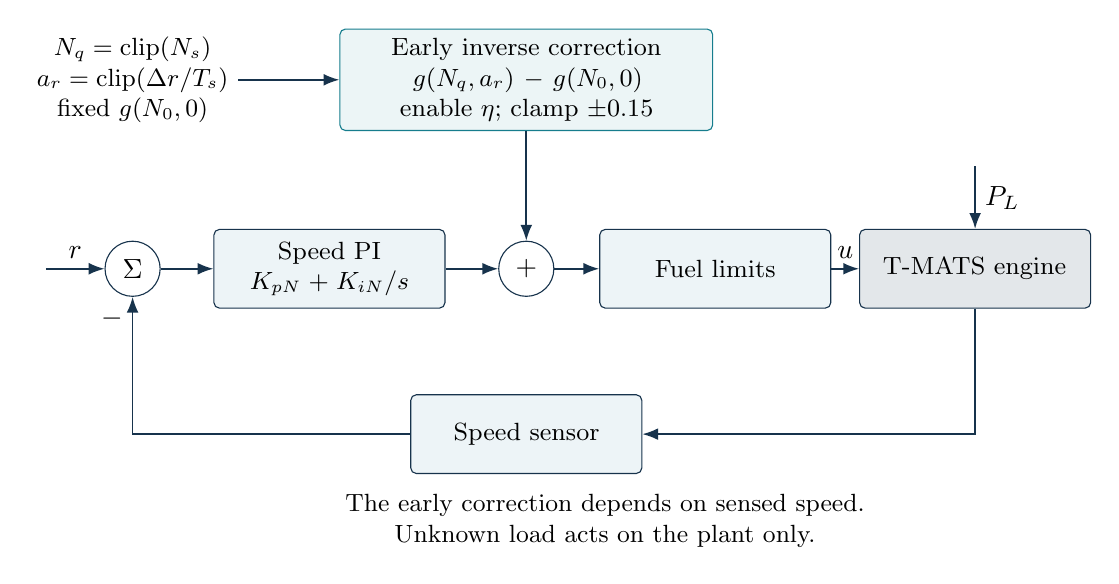
\begin{tikzpicture}[x=1cm,y=1cm]
\node[sum] (e) at (0,0) {$\Sigma$};
\node[block] (pi) at (2.5,0) {Speed PI\\$K_{pN}+K_{iN}/s$};
\node[sum] (add) at (5,0) {$+$};
\node[block] (lim) at (7.4,0) {Fuel limits};
\node[plant] (plant) at (10.7,0) {T-MATS engine};
\node[block] (sensor) at (5,-2.1) {Speed sensor};
\node[gp,text width=45mm] (ff) at (5,2.4) {Early inverse correction\\$g(N_q,a_r)-g(N_0,0)$\\enable $\eta$; clamp $\pm0.15$};
\node[font=\small,align=center] (inputs) at (0,2.4) {$N_q=\mathrm{clip}(N_s)$\\$a_r=\mathrm{clip}(\Delta r/T_s)$\\fixed $g(N_0,0)$};
\draw[arr](inputs)--(ff);\draw[arr](ff)--(add);
\draw[arr](-1.1,0)--node[above]{$r$}(e);\draw[arr](e)--(pi);\draw[arr](pi)--(add);\draw[arr](add)--(lim);\draw[arr](lim)--node[above]{$u$}(plant);
\draw[arr](plant.south)|-(sensor.east);\draw[arr](sensor.west)-|node[pos=.92,left]{$-$}(e.south);
\draw[arr](10.7,1.3)--node[right]{$P_L$}(plant.north);
\node[font=\small,align=center] at (6,-3.2) {The early correction depends on sensed speed.\\Unknown load acts on the plant only.};
\end{tikzpicture}}

\newcommand{\diagramVirtual}{%
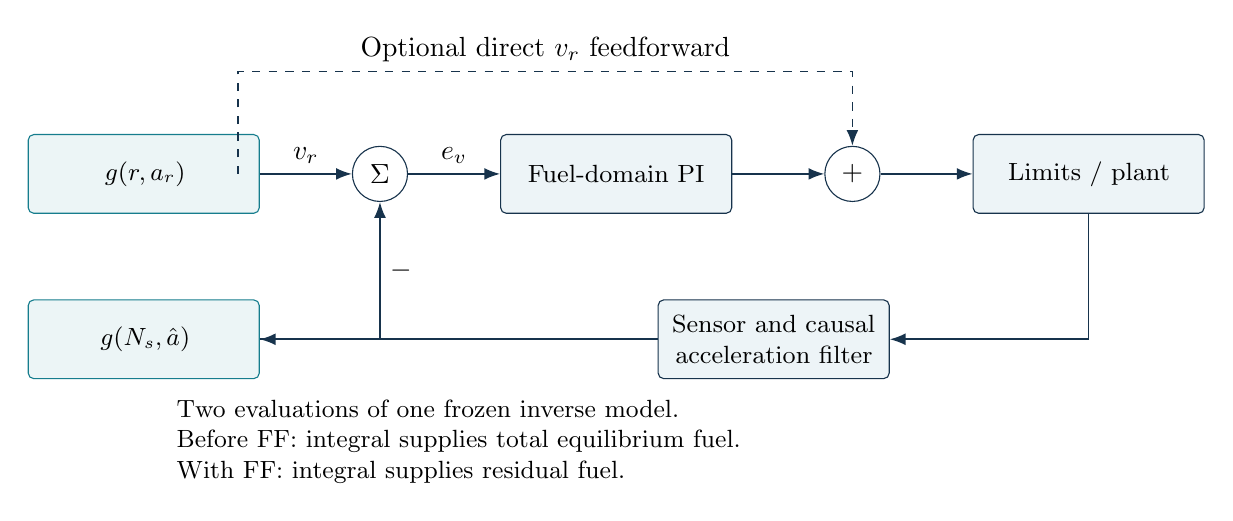
\begin{tikzpicture}[x=1cm,y=1cm]
\node[gp] (r) at (0,0) {$g(r,a_r)$};
\node[sum] (e) at (3,0) {$\Sigma$};
\node[block] (pi) at (6,0) {Fuel-domain PI};
\node[sum] (u) at (9,0) {$+$};
\node[block] (sat) at (12,0) {Limits / plant};
\node[gp] (y) at (0,-2.1) {$g(N_s,\hat a)$};
\node[block] (s) at (8,-2.1) {Sensor and causal\\acceleration filter};
\draw[arr](r)--node[above]{$v_r$}(e);\draw[arr](e)--node[above]{$e_v$}(pi);
\draw[arr](pi)--(u);\draw[arr](u)--(sat);
\draw[arr](sat.south)|-(s);\draw[arr](s)--(y);
\draw[arr](y.east)--(3,-2.1)--node[right]{$-$}(e.south);
\draw[arr,dashed](1.2,0)--(1.2,1.3)--node[above]{Optional direct $v_r$ feedforward}(9,1.3)--(u.north);
\node[font=\small,align=left] at (4,-3.4) {Two evaluations of one frozen inverse model.\\Before FF: integral supplies total equilibrium fuel.\\With FF: integral supplies residual fuel.};
\end{tikzpicture}}

\newcommand{\diagramSchedule}{%
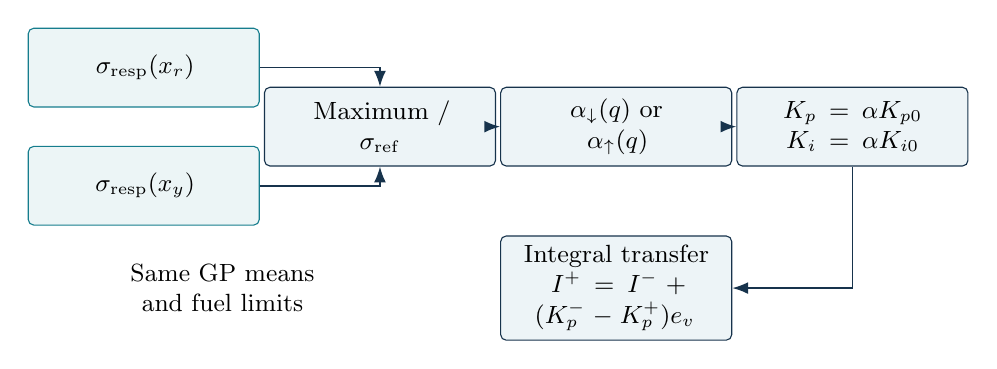
\begin{tikzpicture}[x=1cm,y=1cm]
\node[gp] (sr) at (0,0) {$\sigma_{\rm resp}(x_r)$};
\node[gp] (sy) at (0,-1.5) {$\sigma_{\rm resp}(x_y)$};
\node[block] (mx) at (3,-.75) {Maximum /\\$\sigma_{\rm ref}$};
\node[block] (sc) at (6,-.75) {$\alpha_\downarrow(q)$ or\\$\alpha_\uparrow(q)$};
\node[block] (gain) at (9,-.75) {$K_p=\alpha K_{p0}$\\$K_i=\alpha K_{i0}$};
\node[block] (int) at (6,-2.8) {Integral transfer\\$I^+=I^-+(K_p^--K_p^+)e_v$};
\draw[arr](sr.east)-|(mx.north);\draw[arr](sy.east)-|(mx.south);\draw[arr](mx)--(sc);\draw[arr](sc)--(gain);
\draw[arr](gain.south)|-(int.east);
\node[font=\small,align=center] at (1,-2.8) {Same GP means\\and fuel limits};
\end{tikzpicture}}

\newcommand{\diagramRthree}{%
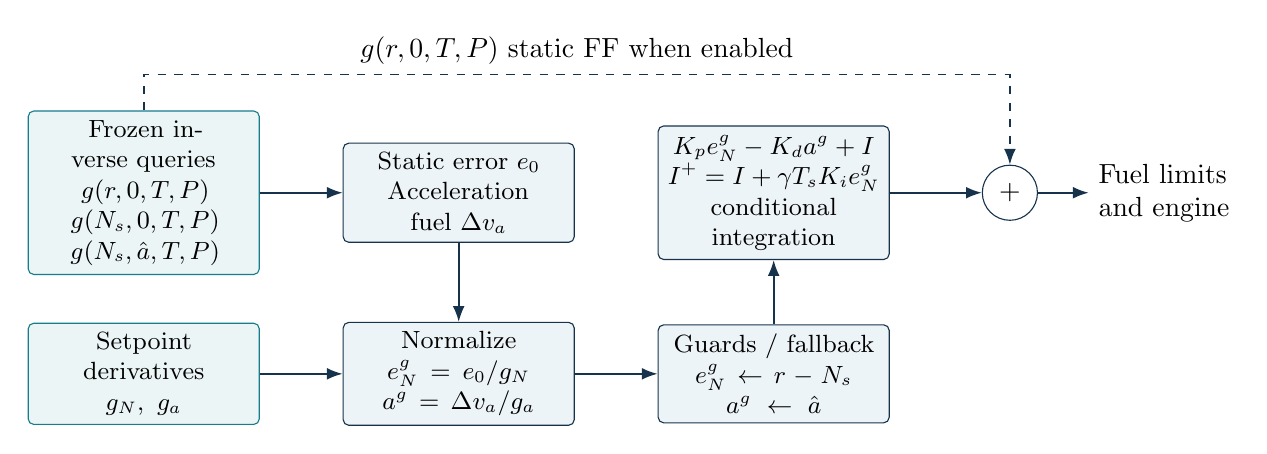
\begin{tikzpicture}[x=1cm,y=1cm]
\node[gp] (queries) at (0,0) {Frozen inverse queries\\$g(r,0,T,P)$\\$g(N_s,0,T,P)$\\$g(N_s,\hat a,T,P)$};
\node[block] (split) at (4,0) {Static error $e_0$\\Acceleration fuel $\Delta v_a$};
\node[gp] (slope) at (0,-2.3) {Setpoint derivatives\\$g_N,\ g_a$};
\node[block] (norm) at (4,-2.3) {Normalize\\$e_N^g=e_0/g_N$\\$a^g=\Delta v_a/g_a$};
\node[block] (guard) at (8,-2.3) {Guards / fallback\\$e_N^g\leftarrow r-N_s$\\$a^g\leftarrow\hat a$};
\node[block] (pid) at (8,0) {$K_p e_N^g-K_d a^g+I$\\$I^+=I+\gamma T_s K_i e_N^g$\\conditional integration};
\node[sum] (sum) at (11,0) {$+$};
\draw[arr](queries)--(split);\draw[arr](split)--(norm);\draw[arr](slope)--(norm);\draw[arr](norm)--(guard);\draw[arr](guard)--(pid);\draw[arr](pid)--(sum);
\draw[arr,dashed](queries.north)--(0,1.5)--node[above]{$g(r,0,T,P)$ static FF when enabled}(11,1.5)--(sum);
\draw[arr](sum)--++(1,0)node[right,align=left]{Fuel limits\\and engine};
\end{tikzpicture}}

\newcommand{\diagramIdentification}{%
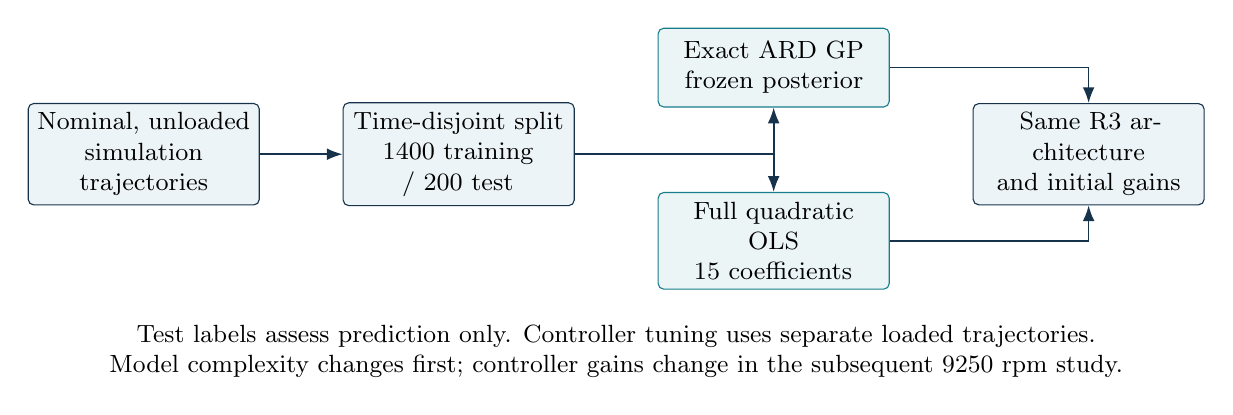
\begin{tikzpicture}[x=1cm,y=1cm]
\node[block] (sim) at (0,0) {Nominal, unloaded\\simulation trajectories};
\node[block] (split) at (4,0) {Time-disjoint split\\1400 training / 200 test};
\node[gp] (gp) at (8,1.1) {Exact ARD GP\\frozen posterior};
\node[gp] (poly) at (8,-1.1) {Full quadratic OLS\\15 coefficients};
\node[block] (ctrl) at (12,0) {Same R3 architecture\\and initial gains};
\draw[arr](sim)--(split);\draw[arr](split.east)-|(gp.south);\draw[arr](split.east)-|(poly.north);
\draw[arr](gp.east)-|(ctrl.north);\draw[arr](poly.east)-|(ctrl.south);
\node[font=\small,align=center] at (6,-2.5) {Test labels assess prediction only. Controller tuning uses separate loaded trajectories.\\Model complexity changes first; controller gains change in the subsequent 9250 rpm study.};
\end{tikzpicture}}

\newcommand{\diagramEvidence}{%
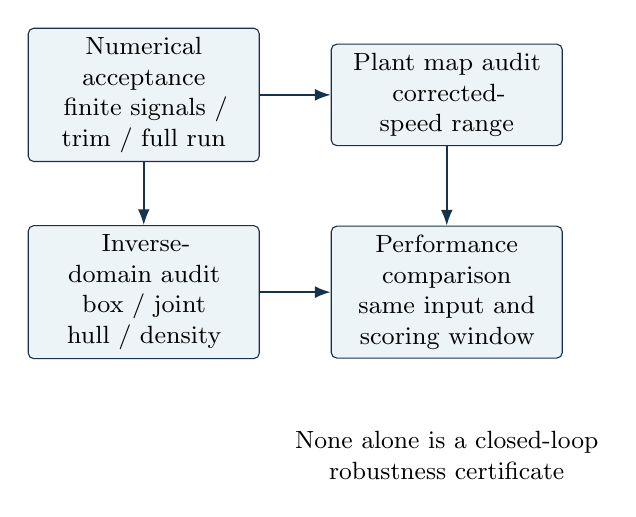
\begin{tikzpicture}[node distance=8mm and 9mm]
\node[block] (a) {Numerical acceptance\\finite signals / trim / full run};
\node[block,right=of a] (b) {Plant map audit\\corrected-speed range};
\node[block,below=of a] (c) {Inverse-domain audit\\box / joint hull / density};
\node[block,right=of c] (d) {Performance comparison\\same input and scoring window};
\draw[arr](a)--(b);\draw[arr](b)--(d);\draw[arr](a)--(c);\draw[arr](c)--(d);
\node[font=\small,align=center,below=8mm of d] {None alone is a closed-loop\\robustness certificate};
\end{tikzpicture}}

\newcommand{\E}{\mathbb{E}}\newcommand{\Cov}{\operatorname{Cov}}\newcommand{\Var}{\operatorname{Var}}


% PDF navigation is added after compilation by the release checker.
\clubpenalty=10000\widowpenalty=10000

\begin{document}
\begin{titlepage}\sffamily\color{navy}
{\large T-MATS RESEARCH / MASTER'S REVISION V2}\par\vspace{12mm}
{\fontsize{27}{33}\selectfont\bfseries\raggedright\hyphenpenalty=10000 Identification, Disturbance Rejection, and Learning-Based Control of a Simulated Gas Turbine\par}
\vspace{9mm}{\Large A comparative study of tracking, fuel-command reversal, and the limits of model-based improvement\par}
\vspace{8mm}\textcolor{teal}{\rule{\linewidth}{1.2pt}}\vspace{7mm}
\normalfont\color{black}
Second edition revised in response to a jury-style assessment. A retrospective, undergraduate-accessible master's-level research report with detailed methods, accepted and rejected experiments, explicit evidence roles, and bounded contribution claims.\par
\vspace{8mm}
\begin{tabular}{@{}ll@{}}
Research direction & Volkan Aran\\[5pt]
Implementation and writing & AI-assisted under human direction\\[5pt]
Plant framework & T-MATS v1.3.3; MATLAB/Simulink R2018b\\[5pt]
Experimental archive & September--October 2026\\[5pt]
Edition date & 11 October 2026\\[5pt]
Revision basis & Written jury-style assessment of Version 1
\end{tabular}
\vfill\textbf{Evidence-only revision.} No new plant simulations, identification fits, controller searches, or Monte Carlo runs were performed. Degree acceptance and independent mastery require a human university examination; neither is asserted by this report.
\end{titlepage}
\pagenumbering{roman}
\chapter*{Abstract}\addcontentsline{toc}{chapter}{Abstract}
This thesis-style report investigates a restricted engineering question: within an archived nonlinear gas-turbine simulation campaign, when do identified or learned models improve the tested control configurations, and which improvements can be attributed to model representation rather than feedback architecture, tuning, or scoring choices? The study is retrospective. It synthesizes existing experiments rather than claiming a newly balanced benchmark or a new control theory.

The plant is a single-shaft T-MATS model with fuel-flow actuation, filtered speed sensing, and optional shaft-power extraction. Numerical acceptance is established before identification or control scores are interpreted. The methods include Wiener and recursive ARX identification, sparse lag selection, filtered-inverse disturbance observers, alternative disturbance estimators, inverse Gaussian-process feedback, polynomial replacement, and PILCO-style offline PI gain optimization. Detailed derivations explain prediction, inversion, implicit feedback action, and an expected excess-variation objective for reducing command reversals.

The principal finding is that improved regression accuracy does not reliably predict improved closed-loop performance in this archive. At one target, derivative-normalized GP feedback has speed RMSE of approximately 1.752 rpm, while a matched filtered PID gives 1.749 rpm; a GP-specific tracking advantage is therefore not demonstrated there. A polynomial inverse remains competitive despite poorer nominal prediction. Adding a ringing penalty reduces the original learned policy's command reversal by about 86 percent in its 10 percent load selection case, but the resulting reversal remains slightly above base PI. The common-sensor audit reproduces prior traces exactly and exposes a reversal of controller ordering between actual-speed and sensed-speed ramp error.

In the final combined cycle, adding DOB98 with original PI gains reduces full-cycle RMSE from 5.408 to 4.546 rpm; subsequent PI retuning reduces it to 3.142 rpm. This is a configured-system improvement on the DOB tuning case, accompanied by greater command reversal and fuel saturation. An equally retuned PI-only comparator is absent, and the model identified near 9800 rpm spans only about 6.3 rpm in its training record. These facts prevent attribution of the complete improvement to the observer architecture or extrapolation to a robust engine-wide guarantee.

The master's-level contribution is an implementation-grounded comparative synthesis: explicit separation of prediction, selection, transfer and implementation checks; analysis of existing ablations; and a reproducible account of favorable, unfavorable and invalid outcomes. The expected excess-variation construction is presented as a technical adaptation whose originality remains unestablished. The revised manuscript narrows its claims accordingly, preserves the full study lineage, and identifies the additional evidence needed for stronger conclusions.

\chapter*{Revision scope and reading guide}\addcontentsline{toc}{chapter}{Revision scope and reading guide}
Version 1 provided a complete chronological research narrative. The written jury-style review judged that the project had substantial master's-level potential but required a focused question, a literature-grounded contribution statement, clearer evidence roles, and stronger attribution discipline~\cite{jury}. Version 2 addresses the documentary and analytical requirements. It does not relabel missing experiments as completed work.

Chapters 1--3 define the question, literature position, and retrospective protocol. Chapters 4--13 provide the physical explanation, mathematical methods and thematic evidence. Chapters 14--15 answer the question and state the defensible conclusions. Appendix A records each examination issue, its resolution or remaining limitation. The other appendices preserve detailed result tables, algorithms, evidence identifiers and the directory register. The original edition remains a separate historical artifact; numerical results are not replaced by newly generated simulations.

The primary reader is assumed to know elementary calculus, linear algebra, and introductory feedback control. Each advanced method is explained from its governing equations before its results are interpreted. Subsection details can be revisited after the main conclusions are understood. A chapter's historical use of the words ``training'' or ``validation'' must be read together with the evidence-role ledger in Chapter~\ref{ch:protocol}; a dataset may be held out from a regression fit while still used to select controller gains.

\textbf{Authorship and examination status.} Volkan Aran directed the project. Implementation, analysis and writing were developed with OpenAI Codex. The jury-style review and the response are AI-assisted documents, not independent human peer review. This report neither certifies candidate independence nor records an oral defence. Mathematical understanding, reproducibility, and authorship responsibility must be demonstrated to an actual examiner. The revision response therefore distinguishes a clarified manuscript from a fulfilled institutional requirement.

\chapter*{Notation and units}\addcontentsline{toc}{chapter}{Notation and units}
\begin{longtable}{p{28mm}p{126mm}}\toprule Symbol & Meaning\\\midrule
$N,N_s,r$ & Actual shaft speed, sensed speed, and governed target; rpm.\\
$u,W_f,I$ & Fuel command/flow and controller integral contribution; lbm/s.\\
$\dot N,\hat a$ & Actual acceleration and causal estimated acceleration; rpm/s.\\
$T_s,q$ & Sample period 0.015 s; one-sample delay $q=z^{-1}$.\\
$T,P$ & Inlet absolute temperature and pressure; K and kPa for inverse models.\\
$P_t,P_c,P_L$ & Turbine, signed compressor, and external extraction power; model hp.\\
$K_p,K_i,K_d$ & Controller gains; units depend on speed or virtual-fuel error definition.\\
$P_n,H,Q$ & Nominal plant, sensor approximation, and observer low-pass filter.\\
$g,p_2$ & Learned inverse GP mean and full quadratic inverse.\\
$\mu,\Sigma$ & Gaussian mean vector and covariance matrix.\\
$R,\mathrm{TV}$ & Excess fuel variation and total variation; lbm/s, not consumed mass.\\
SM, PTO & Available compressor surge margin; external shaft power takeoff.\\
NR & No confirmed recovery within the stated record/band, where used in tables.\\\bottomrule
\end{longtable}
Symbols are reused locally in some historical derivations. Each chapter defines its state and normalization before use. In particular, the GP training matrix and controller gain must not be confused merely because both sometimes use the letter $K$.

\tableofcontents\clearpage\listoffigures\clearpage\listoftables
\clearpage\pagenumbering{arabic}
\chapter{Research question, objectives, and bounded contribution}
\label{ch:question}
\section{The engineering problem}
A speed controller must supply enough fuel to accelerate a shaft and reject unknown external load without producing undesirable fuel-command motion. A PI controller already provides proportional correction and integral rejection of constant error. Adding a learned inverse, a disturbance estimator, or an optimized policy can help, but it can also alter feedback gains, amplify measurement dynamics, or improve a metric that does not represent the physical quantity of interest. The value of a more complicated model must therefore be tested inside the actual feedback loop.

This project originally developed through sequential requests: identification, observers, inverse regression, polynomial replacement, policy optimization, smoother control, ramp transfer, and a final local DOB. Sequential development is normal engineering practice, but its record is not automatically a controlled experiment comparing every method. A retrospective thesis must identify which comparisons isolate a mechanism and which compare complete designs with several differences.

\section{Primary question}
\begin{quote}
Within the archived T-MATS simulation campaign, when do identified or learned models improve the tested controller configurations, and which improvements can the available evidence attribute to model representation, feedback architecture, gain selection, or measurement and scoring choices?
\end{quote}
The phrase ``within the archived campaign'' is a scope condition. It prevents a few successful load cases from becoming a claim about all gas turbines, all operating conditions, or all learning-based controllers. ``Tested configurations'' means the implemented controller, its gains, initialization, filtering, limits and scenario. It is deliberately narrower than an entire method family.

\section{Subsidiary questions and observable answers}
\begin{enumerate}[label=\textbf{RQ\arabic*.},leftmargin=*]
\item \textbf{Prediction and inversion:} Does high one-step or nominal regression accuracy establish a model suitable for free-running prediction and causal inversion? Evidence comes from the Wiener/ARX transfer tests, sparse estimator, inverse-zero audit and local DOB identification.
\item \textbf{Attribution:} Which benefits survive existing controlled substitutions or ablations? Evidence comes from matched-gain feedforward tests, the local matched-PID diagnostic, unchanged-gain GP-to-polynomial replacement and DOB with original PI gains.
\item \textbf{Objective and sensing:} How do tracking, command reversal and controller ordering change when the objective or the scored signal changes? Evidence comes from the ringing-penalty study, metric sensitivity, ramp tests and common-sensor audit.
\item \textbf{Transfer:} How far do the selected configurations retain useful behavior outside their selection case? Evidence comes from independent predictor records, load-amplitude checks, environmental cases, moving-reference cycles and the final frozen-gain check.
\end{enumerate}
These questions were formulated for the retrospective synthesis. They are not described as preregistered hypotheses governing the original campaign.

\section{What the study contributes}
\textbf{C1: A traceable comparative record.} The thesis connects accepted and rejected simulation studies to their models, controller definitions, performance windows and evidence roles. It distinguishes numerical validity, training coverage and control performance rather than treating them as one success criterion.

\textbf{C2: An implementation-level attribution analysis.} Existing ablations show where an apparent benefit can be reproduced by an integral offset, local equivalent PID action, gain selection or a simpler inverse. The mathematical explanations make those mechanisms inspectable. These are application-specific findings and pedagogical derivations, not claims to invent PI equivalence or linearization.

\textbf{C3: A qualified tracking--reversal comparison.} The archive demonstrates multiple tradeoffs rather than one universal winner. It documents the repair of a highly oscillatory learned policy, explains why that repair is not baseline superiority, and retains the final DOB's improved tracking alongside its increased actuator activity.

\textbf{C4: A reproducible technical adaptation.} The expected excess-variation objective is implemented using Gaussian moment propagation with command memory and an event anchor. Its calculation is documented, together with its limitations and verification. The present literature review does not establish a first-in-literature claim. C4 is therefore a reproducible implementation contribution, not an asserted new general theory.

The thesis does not claim that the number of controller variants, figures or pages constitutes originality. Its master's-level value lies in applying established knowledge carefully and deriving defensible conclusions from imperfect experimental evidence.

\section{Claims explicitly excluded}
The work does not establish universal superiority of GP, polynomial, PILCO-style, or observer control over PI. It does not establish an equal-budget optimum across controller families. There is no hardware validation, measured fuel-economy benefit, certified surge-protection envelope, or global robust-stability guarantee. Posterior GP uncertainty is not claimed to bound every physical disturbance. A successful deterministic run is not an independent statistical replicate of a population of engines.

The retained claims do not require missing experiments to be imagined. A comparison can be useful without being decisive. For example, the final DOB-plus-original-PI result demonstrates a change after adding the configured observer to that baseline, while the missing retuned-PI-only branch leaves the observer's advantage over a comparably optimized conventional controller unresolved.

\section{Organization of the argument}
The literature chapter separates established building blocks from the present application. The evidence protocol fixes the vocabulary for fitting, selecting and evaluating them. The technical chapters then explain the sequence of models and controller behaviors. Finally, the cross-study synthesis answers RQ1--RQ4 using the most discriminating existing comparisons, rather than counting the number of favorable cases or averaging incompatible tests. Full historical tables remain in appendices to support audit without defining the thesis argument.

\chapter{Literature position and assessment of originality}
\label{ch:literature}
\section{Review scope and method}
This is a targeted methodological comparison, not a systematic review with an exhaustive database search. The starting points are the methods actually implemented: T-MATS simulation, orthogonal identification, disturbance estimation, inverse GP control, gain scheduling and probabilistic policy search. Primary papers, institutional records and the official simulator documentation provide the comparison. The additional review was checked on 11 October 2026. No absence-of-prior-art conclusion follows merely because an exact phrase was not located.

Two questions organize the comparison. First, which algorithmic elements already exist? Second, what does the present turbine evidence add beyond applying those elements? A different operating speed or a renamed controller is not, by itself, a methodological contribution. Conversely, a carefully demonstrated negative result or a useful application-specific limitation can contribute to engineering understanding without inventing a new algorithm.

\section{Simulation platform and engine-control context}
T-MATS provides the thermodynamic component framework and numerical machinery used to construct the plant~\cite{tmats,tmatsguide}. The present project changes controller and experiment configurations around a particular inherited engine model; it does not develop a new gas-path simulator or validate new component maps. Model-based aircraft-engine control using online estimation also predates this work~\cite{nasaengine}. These sources establish context rather than direct performance comparators: their engines, outputs and objectives differ from the present shaft-speed tests.

The appropriate application claim is therefore specific. This archive documents how a set of identified and learned controllers behaves on the stated T-MATS configuration, including numerical and map limits. It does not claim to introduce model-based turbine control. A fair quantitative comparison with an external paper would require matching the plant, disturbance, actuator constraints and evaluation signal; the present literature chapter does not compare unrelated RMSE values.

\section{Identification and sparse model selection}
Orthogonal least-squares methods combine parameter estimation and structure selection for models linear in their parameters~\cite{ols}. The sparse lag selection in this project is an application of that established family. Its relevant evidence is the recorded reduction in conditioning problems, smaller retained structure, and held-out performance relative to the ten-term model. A smaller covariance matrix is an implementation simplification, but it does not constitute a measured real-time speedup. The block realization and recurrence replay show that the estimator was implemented correctly; they do not create a new identification algorithm.

\section{Disturbance observers and related estimators}
Filtered inverse-model DOB control estimates an equivalent input disturbance and compensates it through the control channel. Its relationship to alternative disturbance-estimation methods is well established~\cite{doboverview}. LESO and UDE likewise have prior formulations and tuning principles~\cite{gao,ude}. The application choices here are the identified model, equilibrium correction, causal filter, compensation limit, startup procedure and gain selection.

The contribution is not ``DOB plus PI'' as a new architecture. It is the account of why a raw acceleration inverse was unsuitable, how the filtered implementation was constructed, and what the accepted cases demonstrate. The final 9800-rpm model is a different local nominal approximation, not a new class of observer. Its combined-cycle improvement must be assessed together with its narrow identification range and the missing equally retuned PI-only branch.

\section{GP regression, feedforward and inverse coordinates}
Gaussian-process regression supplies a posterior mean and variance conditional on specified statistical assumptions~\cite{gpml}. Prior work already applies GP feedforward to diesel-engine airpath control~\cite{aran}; the related doctoral thesis establishes part of the project's intellectual lineage~\cite{aranthesis}. This turbine study concerns a different simulated plant and different test sequence. It neither duplicates those physical results nor claims GP feedforward for engine control as a new concept.

The more informative question is how an inverse is used. A map used only to supply a nominal command differs from a map queried using measured speed and acceleration inside feedback. The latter can change effective proportional, integral and derivative action. The present derivations expose that mechanism, and the matched-PID diagnostic tests whether a GP-specific benefit remains at a selected operating point. That diagnostic limits the novelty and performance claim even though the GP fit is excellent.

The uncertainty schedules are empirical design hypotheses. Gain scheduling itself has a substantial literature~\cite{scheduling}. The presence of a GP standard deviation does not automatically determine whether gains should increase or decrease, especially when the posterior omits unknown-load mismatch and physical uncertainty. The thesis presents the measured tradeoffs without promoting the schedules into a general robustness rule.

\section{PILCO and the restricted implementation used here}
Original PILCO-style PI combines a learned probabilistic dynamics model, approximate long-horizon inference and analytical policy gradients, with iterative data collection and policy improvement~\cite{pilco}. Later work further develops GP-based data-efficient control~\cite{deisenroth}. In this project, historical transition data are fitted offline, feedforward coefficients are fixed, and only two PI gains are optimized with numerical gradients. A 40-point representative GP approximation and an affine unsaturated planning policy are used, while the nonlinear plant deployment includes fuel limits and conditional integration.

The accurate description is \emph{PILCO-style GP-based offline PI tuning}. The study does not claim a reproduction of the full original learning loop, an improvement in sample efficiency over original PILCO, or analytic policy gradients. Its useful evidence concerns what this restricted probabilistic tuning procedure selected and how that policy transferred to the recorded plant scenarios.

\section{Smooth actions and the excess-variation adaptation}
CAPS regularizes temporal and spatial action variation to obtain smoother learned control~\cite{caps}. It therefore precedes the broad idea of penalizing irregular learned commands. The present objective is different in detail: event-window total variation minus absolute net command change, evaluated in expectation under an augmented Gaussian state. CAPS and the present construction do not use identical policies or experiments, so the literature comparison establishes related purpose rather than numerical superiority.

For a Gaussian scalar $Z$ with mean $\mu$ and variance $v$, the absolute first moment used by the project is
\begin{equation}
\mathbb E|Z|=\sqrt{\frac{2v}{\pi}}\exp\!\left(-\frac{\mu^2}{2v}\right)+\mu\,\operatorname{erf}\!\left(\frac{\mu}{\sqrt{2v}}\right),\qquad v>0.
\end{equation}
At zero variance it is $|\mu|$. This is a mathematical property of the Gaussian distribution, not a newly discovered moment formula. The implementation combines it with command-memory covariance and event-anchor resets. That combination is a candidate incremental adaptation; originality is not established by the present targeted search. Its value over ordinary total variation or a squared-increment cost was not tested under an equal selection protocol.

\section{Contribution matrix}
\begin{longtable}{@{}p{.22\linewidth}p{.31\linewidth}p{.40\linewidth}@{}}
\toprule Element & Established basis & Contribution retained in this thesis\\\midrule\endhead
Wiener, ARX and sparse estimation & Existing identification and structure-selection methods & Recorded conditioning, prediction and realization comparisons for this plant.\\
Filtered inverse DOB & Existing residual estimation and low-pass compensation & Explicit inversion constraints, local implementations, partial observer/tuning ablation.\\
GP feedforward and inverse feedback & Existing regression and engine feedforward concepts & Analysis of feedback-coordinate effects and limits of prediction-based ranking.\\
R3 and matched PID & Local normalization and conventional PID action & Evidence that target improvement is not demonstrably GP-specific.\\
Polynomial replacement & Standard quadratic regression & Same-architecture challenger showing competitive control despite poorer fit.\\
PILCO-style PI search & Established probabilistic model-based policy evaluation & Offline two-gain adaptation with declared planning/deployment differences.\\
Expected excess variation & Known absolute moments and smooth-action motivation & Reproducible event-window adaptation; originality unestablished.\\
Complete comparative record & Established scientific reporting principles & Traceable evidence of metric-dependent and scenario-dependent outcomes.\\\bottomrule
\end{longtable}

\section{The defensible gap}
The gap addressed is \emph{within this project}: why did more elaborate models fail to improve consistently over inherited PI? The answer separates prediction, feedback action, tuning, sensing and coverage. This application-specific synthesis supports a master's contribution. A broader novelty claim would require additional prior-art review and discriminating evidence.

\chapter{Retrospective evidence protocol and comparison rules}
\label{ch:protocol}
\section{What was and was not changed for Version 2}
The revision reorganizes and explains an existing record. No plant trajectory, model fit, controller gain, penalty-weight search or Monte Carlo sample was newly generated. Numerical values are copied from the archived reports and saved summaries. Derived percentages and algebraic explanations are interpretation of existing results. The original report, source evidence index and revised source manifest remain available to identify the provenance of those results.

The archive contains 69 result directories, not 69 independent replications. Some directories are pilots, failed runs, replays, aggregates or presentation outputs. The study register identifies them individually. Deterministically repeating a simulation checks repeatability of the implementation; it does not create an independent sample of engine-to-engine uncertainty.

\section{Evidence roles}
\textbf{Fitting} estimates model parameters from observations. \textbf{Selection} chooses a model order, gain set, architecture remedy or penalty weight using observed performance. \textbf{Held-out prediction} evaluates a predictor on a record excluded from the relevant fit. \textbf{Frozen-controller transfer} applies previously selected parameters to another condition without retuning. \textbf{Ablation} changes a specified component while retaining the other stated conditions. \textbf{Implementation verification} checks equations or code against a reference calculation. These labels describe different questions, not a ranking from bad to good.

A dataset can have more than one role at different stages. The third pulse may be excluded from a GP fit, but if a full test containing it is later used to choose a ringing penalty, that test is no longer held out from policy selection. A comparison can also be a transfer test for one controller and a selection case for another. The final combined cycle is exactly such a case.

\section{Evidence-role ledger}
The following ledger is the controlling interpretation of the historical terminology used in later chapters. ``Independent'' refers to the stated record or selection step, not to a new engine or a statistically independent set of every time sample.

\small
\begin{longtable}{@{}p{.19\linewidth}p{.27\linewidth}p{.23\linewidth}p{.23\linewidth}@{}}
\toprule Study & Fitting or selection role & Evaluation role & Permitted inference\\\midrule\endhead
Numerical baseline, steps, chirp and PRBS & Excitation feasibility; requested full records can fail & Accepted trajectories/prefixes assessed for residuals and finite signals & Defines usable data; failed full records are not successful controls.\\
Wiener models & Accepted chirp used for fitting; selection ramp chooses among candidates & Separate held-out ramp & Prediction within these records; not engine-wide validity.\\
Ten-term RLS & Online coefficient updates on the chirp & Frozen chirp and held-out ramp; block replay & Separates one-step adaptation, free-run transfer and implementation.\\
Sparse RLS & Offline lag-support selection, then coefficient estimation & Held-out ramp; conditioning and recurrence checks & Local comparison of retained structures, not a new online support learner.\\
Early DOB & Identified model, equilibrium constraint and filter design & Governed-reference and input-disturbance scenarios & Configured observer behavior under stated excitations.\\
PTO observer tests & Established configurations; scenario progression is adaptive & Operating-point/load checks, including invalid runs & Local envelope and paired differences; not a common-power cross-speed ranking.\\
Two-input forward/inverse GP & 600 nominal training points & 100 points from a separate experiment & Nominal prediction; temporal samples are not independent engine trials.\\
Virtual-fuel PI and FF retune & Architecture and gains evolve together & Fixed-load cases and same-gain FF ablations & Combined-design results; only the ablation isolates FF.\\
SD schedules and lower gains & Empirical scheduling direction and local gain selection & Accepted/rejected load cases & Tracking/reversal tradeoffs; no uncertainty-based safety guarantee.\\
Four-input GP & 1400 training points across 35 ambient conditions & 200 test points across 33 conditions & Nominal interpolation evidence; not loaded-plant uncertainty bounds.\\
R1--R3 remedies & 80 candidates selected at the target case & Target table, frozen environmental grid, matched PID & Target is selection evidence; grid and matched PID answer distinct transfer/attribution questions.\\
Broad moving cycle & Frozen controller applied to expanded task & Coverage and performance audit & Stress/transfer evidence with out-of-domain exposure.\\
Covered moving cycle & Scenario narrowed after broad-cycle diagnostics & Matched controller and FF comparisons & Performance within the resulting tested coverage; not a blind generalization test.\\
GP-to-Poly2 substitution & Same nominal training data; gains initially retained & Same covered cycle & Representation comparison within one architecture.\\
9250-rpm Poly2 retune & 28 initial candidates plus six refinements on 10\% pulses & Frozen 5\% pulses; saved-metric sensitivity & Local selection plus amplitude transfer; 9250 rpm is below old training minimum.\\
Original PILCO-style PI & 4242 historical transitions; 40-point representative GP; two-gain optimization & Third-pulse GP holdout and nonlinear load comparison & Restricted offline model-based tuning; distinguish predictor holdout from policy evaluation.\\
Smooth PILCO-style PI & GP reused; penalty weight selected with 10\% full-test results & 5\% case excluded from policy selection & Repair of ringing on selection case; limited amplitude transfer.\\
No-load ramp and sensor audit & Earlier controllers frozen & Five-second ramp; explicit equal-sensor replay & Task transfer and sensing audit, not new gain optimization.\\
Initial combined cycle & Earlier controllers frozen & Five-second ramp plus load at seconds 10--15 & Common-scenario transfer comparison.\\
DOB98 local model & Fuel PRBS around 9800 rpm; least-squares fit & Separate local multisine & Local predictor fit over a few rpm.\\
DOB98 PI search & 13 PI candidates with fixed DOB on combined cycle & Original-gain ablation; frozen 4 s ramp/5\% pulse check & Main cycle is selection evidence; second case lacks a full comparator lineup.\\
Moment and algebra checks & No controller evidence added & Recurrence, inverse identity and GP Monte Carlo comparisons & Correctness of stated computations, not physical robustness.\\\bottomrule
\end{longtable}
\normalsize

\section{What a matched comparison requires}
The common plant, reference and load are necessary but insufficient for equal opportunity. A controller also depends on sensing, sample interval, initialization, gain-selection budget, clipping, anti-windup, and the objective used for selection. When those factors differ, the correct statement is ``configuration A performed better than configuration B on this case.'' It is not ``method A is intrinsically better.''

The existing record contains several more controlled comparisons. Constant-reference FF tests match gains and integral offsets. The GP-to-polynomial substitution initially holds architecture and gains fixed. The common-sensor audit replays the same controllers with explicit common settings. The DOB original-gain result changes the observer while retaining the inherited PI gains. Each controls a particular source of ambiguity; none controls every source across the full project.

The matched filtered PID is a local diagnostic. Its near-equality with R3 at the target shows that a more conventional implementation can reproduce that target behavior. It does not prove all GP controllers are equivalent to PID at all operating points. Similarly, a favorable unchanged-gain polynomial result does not prove that every possible GP architecture is unnecessary.

\section{Primary response and phase weighting}
Unless a table explicitly states otherwise, tracking is scored using actual shaft speed $N$, while the controller uses sensed speed $N_s$. Define
\begin{equation}
E_N=\sqrt{\frac{1}{M}\sum_k(N_k-r_k)^2},\qquad
E_s=\sqrt{\frac{1}{M}\sum_k(N_{s,k}-r_k)^2}.
\end{equation}
Neither value should be substituted for the other. In the deterministic simulator, actual speed is available for evaluation even though the controller receives a lagged signal. Hardware would require an independently justified measurement or estimate of the physical quantity.

For disjoint phases $j$ with sample counts $M_j$, full-record RMSE obeys
\begin{equation}
E_{\rm full}^2=\sum_j\frac{M_j}{\sum_iM_i}E_j^2.
\end{equation}
It is not the arithmetic mean of phase RMSEs. A design can worsen the ramp and improve the full score because the other phases are longer or their large deviations dominate the sum of squares. This is central to the final DOB retune. Phase endpoints in an actual replay must follow the original masks; a boundary sample should not silently be counted twice when reconstructing a disjoint decomposition.

\section{Fuel command, reversal and recovery}
For a prescribed event window $a{:}b$,
\begin{equation}
R_{a:b}=\sum_{k=a+1}^{b}|u_k-u_{k-1}|-|u_b-u_a|.
\end{equation}
The triangle inequality gives $R_{a:b}\ge0$. This is accumulated excess change in a flow signal, measured in lbm/s. It is not fuel mass, which would be approximately $T_s\sum_k u_k$. Nor is it a bound on slew, $\max_k|u_k-u_{k-1}|/T_s$. A sudden monotonic transition has zero excess variation but may have high slew. These quantities are reported as different performance dimensions.

Excess variation depends on event boundaries. Splitting a signal into several windows changes the subtracted endpoint terms. The final DOB objective uses segmented variation across ramp and load phases; the load-only table reports a subtotal. Both can be correct while numerically different. Noise and sampling also affect variation, so results are compared using the original common sample interval and stated windows.

Recovery needs an error band and persistence rule. Zero recovery under a wide band may mean the trajectory never left the band, not instantaneous correction. The saved sensitivity analysis shows that changing the band can reverse the original-versus-retuned Poly2 ordering. No universal settling-time superiority is inferred.

\section{Numerical and operating-domain acceptance}
Converged flow residuals establish satisfaction of the numerical equations at the prescribed tolerance. Compressor-map inclusion concerns the thermodynamic model's intended domain. GP box or convex-hull inclusion concerns nominal regressor coverage. Available surge margin is a simulated output. These checks do not imply one another, and none alone proves robust physical safety.

Failed full trajectories remain failed full trajectories. An accepted prefix can be used for an explicitly delimited identification task, as with the chirp, but cannot be reported as a successful completion of the requested full excitation. Invalid runs are retained in acceptance counts and shown as unscored where appropriate. They are not replaced by zero error or excluded without explanation.

\section{Statistical interpretation}
The nominal simulations are deterministic, and samples along a trajectory are temporally related. No p-value or confidence interval is constructed by pretending that every sample is an independent experiment. Small differences such as the target R3/matched-PID gap are reported as observed numerical differences, not statistically significant population effects. Confidence in reproducibility comes from preserved inputs, trajectories, code and checks; confidence in generalization would require a separately designed range of conditions and uncertainty realizations.

\section{Why missing comparisons remain missing}
No equal-budget PI-only search, sensor-noise sweep, actuator-lag sweep, or independent-engine test was added. Version 2 addresses the jury's concern by limiting claims to the evidence that exists. If architectural superiority is later claimed, a new experiment must first equalize selection objectives, constraints and evaluation conditions. The proposed design in Chapter~\ref{ch:conclusions} is a future protocol, not a retroactive description of the present archive.

\chapter{Plant, sensing, metrics, and numerical acceptance}
\label{ch:plant}
This chapter specifies the physical and numerical experiment. Numerical acceptance precedes controller ranking: a failed flow solution is not a valid response to score. Historical experiments are described retrospectively; no test was rerun for Version 2.

\section{Physical plant and feedback foundations}
\subsection{From fuel to shaft speed}
A gas turbine converts chemical energy into hot-gas energy and then shaft work. Air enters through the inlet, is compressed, receives heat in the burner, expands through the turbine, and exits through the exhaust system. The turbine drives the compressor on the same shaft. Their powers are individually large even when the shaft speed is constant. Steady speed means their signed net power balances the external extraction and losses; it does not mean either component has zero power.

The model is a single-shaft turbojet built from T-MATS components. Its gas-path sequence includes ambient/inlet, compressor, burner, turbine, duct, and nozzle. Component maps encode relationships such as flow, pressure ratio, efficiency, and corrected speed. These maps are part of the plant, not learned by the controller. T-MATS is the modeling framework; the particular component maps and model setup define the specific simulated engine~\cite{tmatsguide}.

Let angular speed be $\omega=2\pi N/60$, where $N$ is in rpm. Rotational mechanics gives
\begin{equation}J\dot\omega=\tau_t+\tau_c-\tau_L,\qquad P=\tau\omega.
\end{equation}
With compressor power entered using its signed convention, the project's shaft equation is
\begin{equation}
\dot N=\frac{60}{2\pi J}\,5252.113\frac{P_t+P_c-P_L}{N},\qquad J=30.
\end{equation}
The numerical conversion belongs to the archived horsepower/rpm and inertia convention. It must not be combined blindly with SI torque. This equation explains the sign of a load transient: increasing $P_L$ makes the net power negative, the shaft decelerates, and feedback raises fuel until turbine power restores balance. When the load is removed, the previously increased fuel initially creates excess power and overspeed.

\subsection{Why the nonlinear solver matters}
At each integration step, gas-path flows must agree across connected components. An inner Newton--Raphson calculation adjusts variables such as inlet flow, compressor map coordinate, and turbine map pressure ratio to reduce three flow residuals. The outer integration advances the shaft state. Thus a smooth-looking speed trace can coexist with an internally failed flow solve. Reporting speed alone would miss this failure.

The baseline setup uses fixed-step ode4, $T_s=0.015$ s, normalized flow tolerance $10^{-9}$, and an iteration ceiling of 200. A residual below tolerance means the algebraic flow equations were solved to the prescribed numerical accuracy. It is not a measurement of physical model uncertainty. Conversely, failure to converge is not by itself proof that a real compressor surged. Map warnings, available surge margin, finite signals, and convergence each answer a different question.

The initial baseline archive verifies that the GPT copy matches the supplied standard model by SHA-256. Later experiments create named variants. Copying the plant allows a controller subsystem to change while retaining the gas path; it does not excuse checking sensor connections, initialization, solver settings, or actuator limits. Those details eventually became central to the ramp comparison.

\subsection{Signals, units, and operating points}
Three speed signals must remain separate: requested speed, governed reference $r$, and actual mechanical speed $N$. The sensor output $N_s$ is the feedback measurement. A rate governor can make $r$ a ramp even if the raw request is a step. The controller generally receives $N_s$, while performance tables primarily score $N-r$. In this report the feedback error is $e=r-N_s$ unless explicitly stated otherwise; signed plotted tracking error may instead be $N-r$.

Fuel flow $u=W_f$ is in lbm/s. Turbine and extraction powers are in hp in the model, with MW sometimes reported for interpretation. Temperatures from the station buses are absolute Rankine and convert as $T_K=(5/9)T_R$. Absolute pressure converts from psia to kPa by multiplication by 6.894757. Mixing absolute and gauge pressure, or Celsius and Kelvin, would corrupt an inverse model even if the regression code were correct. Altitude units are also recorded separately from the controller's temperature and pressure inputs.

Rated speed in the October tests is defined as 10000 rpm. Therefore 90\%, 98\%, and 100\% denote 9000, 9800, and 10000 rpm. They are not model-fit percentages and are not compressor-map corrected-speed coordinates. A local model identified at 9800 rpm is therefore a model around a physical operating point, not a model with an asserted 98\% accuracy.

\subsection{PI action explained from the equation}
An ordinary PI controller uses
\begin{equation}u^*=K_p(r-N_s)+I,\qquad \dot I=K_i(r-N_s).
\end{equation}
The proportional term responds immediately to the current error. The integral term remembers accumulated error and supplies the persistent fuel offset needed to balance an unknown constant load. If the shaft stays below target, the integral grows until the error can disappear. This is why adding a constant feedforward value at a fixed operating point need not improve a well-initialized PI controller: the integral can already provide that constant.

The inherited speed controller uses $K_p=0.025$ and $K_i=0.05$. Their units differ: $K_p$ converts rpm into lbm/s, whereas $K_i$ converts rpm-seconds into lbm/s. A virtual-fuel PI later uses different error units, so its numerical gains cannot be compared directly with these speed-PI gains. Initial integral state is also part of the controller. The standard starting value is not automatically the equilibrium fuel for every requested speed; preparation intervals allow the engine and controller to settle.

Fuel saturation clips a requested command into the allowable range, commonly $0.2\le u\le4$ lbm/s in the augmented studies. If an integrator keeps accumulating positive error while fuel is already at its maximum, it stores an unrealizable command. Conditional integration prevents updates that push farther into saturation and permits updates that unwind it. Some early studies intentionally retain the original PI without adding anti-windup; later implementations explicitly implement it. The report therefore does not assume one universal anti-windup law across the whole archive.

\subsection{Sensor lag, differentiation, and causality}
A first-order sensor satisfies approximately $\tau_s\dot N_s+N_s=N$. Its output cannot instantly follow changing true speed. With $\tau_s=0.05$ s and a constant acceleration of 200 rpm/s, the continuous steady ramp lag is approximately $\tau_s\dot N=10$ rpm. Sampling and signal timing can add to the observed lag. This simple calculation will help interpret the October ramp test.

Backward differencing gives a causal acceleration estimate $(N_{s,k}-N_{s,k-1})/T_s$. Causal means using only current and previous samples, never future measurements. Differencing amplifies rapid measurement changes, so filtered acceleration is used in later controllers. The ideal direct plant acceleration used for early identification is not automatically available to a deployed controller. Keeping those two information sets distinct prevents an unrealistically favorable controller comparison.



\section{Experimental design and the first numerical boundary}
\subsection{What constitutes a valid comparison?}
A comparison should hold plant, sensor, reference, load, sample interval, preparation, and scoring rules fixed while changing the intended controller feature. If gains also change, the result establishes the performance of the whole configured design; it does not isolate the contribution of a newly added model. An ablation changes one feature while holding the others fixed. A transfer test evaluates frozen parameters in another scenario. A tuning test supplies evidence used to select the parameters and cannot simultaneously serve as independent validation.

The archive contains baseline attempts, failed excitation studies, final accepted studies, intermediate pilot folders, analysis-only aggregates, and presentation artifacts. They are all part of the project history, but they are not equally independent evidence. The final directory register lists them explicitly. Repeated copies in the two Git repositories are distribution copies, not extra trials. Empty pilot directories supply no empirical support.

\subsection{Metrics and their different meanings}
For $M$ samples and actual-speed error $e_k=N_k-r_k$,
\begin{equation}\RMSE=\sqrt{M^{-1}\sum_{k=1}^M e_k^2},\quad
\mathrm{IAE}=T_s\sum_{k=1}^M|e_k|,\quad E_{\max}=\max_k|e_k|.
\end{equation}
RMSE emphasizes large errors through squaring. IAE measures accumulated absolute deviation. Peak error addresses the worst excursion. A controller can improve one while worsening another. With unequal phase durations, full-record RMSE weights a long hold more than a short ramp. Phase-specific scores are therefore necessary in a combined cycle.

Model fit in the identification chapters is
\begin{equation}\mathrm{Fit}=100\left(1-\frac{\|y-\hat y\|_2}{\|y-\bar y\|_2}\right).
\end{equation}
It is not $R^2$, which uses squared norms. The denominator changes across datasets, so a smaller RMSE can coexist with a lower fit percentage when the new reference varies less. A 99\% one-step acceleration fit does not mean a controller tracks speed within 1\%.

Fuel total variation is $\sum|u_{k+1}-u_k|$. Subtracting absolute net change gives excess variation, a command-reversal measure. Integrating $u$ over time instead gives fuel mass. These are different physical quantities. Recovery time also needs a declared band and persistence rule; a trajectory that never leaves a wide band has zero recovery by that definition even if its fine regulation is visibly poor.

\subsection{Baseline and step attempts}
The accepted baseline holds 10000 rpm for 5 s, ramps toward 9000 rpm by 10 s, and runs to 10.5 s. Its 701 samples have maximum flow residual $9.9891\times10^{-10}$ and at most 20 inner iterations. Final speed is 8998.3405 rpm, fuel 0.9970915 lbm/s, and thrust 4380.7032 lbf. The final speed is recorded at a finite time, not claimed to be a fully settled equilibrium.

A 10 rpm step from 10000 to 9990 rpm at 1.5 s completes the 3 s test with 201 samples, maximum residual $9.7587\times10^{-10}$, and at most 14 iterations. The earlier 100 rpm downward step reaches the 200-iteration ceiling and a residual around 0.37016, accompanied by singular-Jacobian or map warnings. Reducing the step demonstrates a numerically acceptable local experiment, not a universal permissible step-size limit. The failed run is retained as a diagnostic rather than scored as successful control.

\subsection{Why the requested chirp could not be used in full}
The requested chirp is
\begin{equation}r(t)=9500-500\cos\{2\pi(0.1t+0.0075t^2)\}.
\end{equation}
Its instantaneous frequency is $0.1+0.015t$ Hz, reaching 1 Hz at 60 s. A constant speed amplitude does not imply a constant acceleration demand: differentiating the phase shows that the required speed rate grows with frequency. The controller must generate increasingly rapid fuel changes even though the visible speed bounds remain 9000--10000 rpm.

After 30 s preparation, the first invalid sample occurs at chirp time 17.805 s, near 0.367075 Hz. Only the 1187 samples through 17.790 s are accepted. Subsequent negative fuel and solver failures are diagnostic data. Every later model trained on this record must be described as trained on the valid prefix, not on a successful 60 s, 0.1--1 Hz sweep. This restriction is preserved in the Wiener, RLS, and early GP narratives.

\subsection{PRBS, rate limiting, and independent ramps}
A pseudo-random binary sequence excites a system using deterministic switches between two levels. The project's 127-bit sequence follows $b_{k+7}=b_k\mathbin{\mathrm{xor}}b_{k+3}$ with seed 0110101. The full-amplitude 9000/10000 rpm, 0.51 s/bit test fails at its first edge, leaving only 34 valid samples. Timing adjustments in a repeat addressed breakpoint alignment, not the basic numerical difficulty of the large abrupt transition.

Later studies use governed binary requests or small-amplitude binary steps. Once a governor turns a step into a ramp, the applied reference is no longer a strict PRBS. This matters because the actual frequency content delivered to the plant is altered. The model-identification input is actual fuel, not simply the raw binary request.

Independent ramp-and-hold records supply accepted selection and validation data. Their rates include 50, 60, 95, 100, and 150 rpm/s. Holds expose equilibrium errors that a rapidly varying chirp can conceal. Separating the selection record from the final validation record allows model order or lag support to be chosen without consuming the final test. This design decision links the failed excitation phase to the more credible identification studies that follow.



\section{Identification primer: dynamics, regressors, and prediction}
\subsection{A model is an approximation with an information pattern}
A dynamic model predicts future output from stored state or past signals. A static regression predicts an output from a current input vector. Neither description alone specifies how the model will be used. In a one-step predictor, measured past outputs are available at every sample. In free-running prediction, the model must recursively use its own predicted outputs. An error can therefore accumulate rather than being corrected by the next measurement.

For an ARX model, with $q$ a one-sample delay,
\begin{equation}A(q)y_k=B(q)u_k+\epsilon_k,\quad
A(q)=1+\sum_i a_iq^i,\quad B(q)=\sum_jb_jq^j.
\end{equation}
Rearranging gives $\hat y_k=\phi_k^\top\theta$, where the regressor contains negative past outputs and delayed inputs. The signs are a convention inherited from moving the output terms to the right-hand side. A lag of ten samples here means 150 ms, not ten seconds. Normalizing signals improves numerical conditioning but requires restoring physical units before using coefficients in a controller.

\subsection{Least squares and recursive least squares}
Stacking observations gives $y=\Phi\theta+\epsilon$. Least squares minimizes $\|y-\Phi\theta\|^2$. If columns of $\Phi$ are almost redundant, many coefficient combinations predict nearly the same output. A high condition number warns that small perturbations can change individual coefficients substantially. Excellent prediction is therefore compatible with poorly identified parameters.

Recursive least squares updates a previous estimate using the new prediction error:
\begin{align}
P_k^-&=P_{k-1}/\lambda,&
L_k&=\frac{P_k^-\phi_k}{1+\phi_k^\top P_k^-\phi_k},\\
\theta_k&=\theta_{k-1}+L_k(y_k-\phi_k^\top\theta_{k-1}).
\end{align}
Here $P$ is an information-related covariance matrix and $\lambda$ discounts older data. The implementation uses a Joseph-form update,
\begin{equation}P_k=(I-L_k\phi_k^\top)P_k^-(I-L_k\phi_k^\top)^\top+L_kL_k^\top,
\end{equation}
followed by symmetrization. This is a numerical safeguard, not proof that $P$ is a calibrated physical uncertainty interval. At $\lambda=0.999$, the approximate memory scale $1/(1-\lambda)$ is 1000 samples or 15 s.

Publishing the prediction before updating with the current output prevents leakage. Otherwise the purported one-step prediction would already have used the answer. Similarly, a validity gate must stop parameter updates once the reference plant fails. In this project the failure latch freezes coefficients and history and returns undefined predictions for the failed remainder.

\subsection{Wiener models and sparse lag selection}
A Wiener model cascades linear dynamics with a static nonlinear output map. In this project a quadratic output nonlinearity can bend the linear dynamic response to represent a changing input-output relationship. It is a different modeling assumption from a static map of speed and acceleration to fuel. Its memory lives in the linear block, while its output nonlinearity has no independent dynamics.

Sparse lag selection asks which past samples add nonredundant information. The two-stage RLS study first screens a dictionary of possible delays, then estimates coefficients for the retained support. Because support is chosen using the full training record, this is offline structure selection followed by recursive coefficient replay; it is not a fully online algorithm that discovers structure causally. This distinction does not diminish the conditioning improvement, but it defines the claim accurately.

\subsection{What identification can establish}
The following chapters report progressively different successes: a useful Wiener free-run speed model, a highly accurate one-step acceleration predictor, a smaller and better-conditioned sparse predictor, and finally models suitable for filtered inversion. These are not interchangeable achievements. A model selected for one-step accuracy can have an unsuitable DC gain or a nonminimum-phase zero. Such defects become important only when the model is placed inside feedback, motivating the first disturbance-observer study.



\chapter{Identification quality and the limits of prediction}
\label{ch:identification}
The first subsidiary question asks what can be inferred from a high prediction score. The following studies distinguish a fitted output map, online one-step prediction, frozen free-running prediction, and an implementable estimator. These are different achievements. Orthogonal term selection is an application of established identification ideas~\cite{ols}; the contribution here is the recorded comparison and implementation.

\section{Wiener identification: a nonlinear output map after linear dynamics}
\textit{Evidence basis: }\path|results/wiener_ramps_20260908_214558_458/REPORT.md|. The following detailed account is adapted from the archived study; references to simulation and verification describe historical work.\par

Fitted in MATLAB R2018b, System Identification Toolbox 9.9, using \path|nlhw|,
\path|unitgain| on the input and \path|poly1d(2)| on the output.

\subsection{Selected model and free-run fits}

{\scriptsize\setlength{\tabcolsep}{1.5mm}\begin{longtable}{>{\raggedright\arraybackslash}p{50.33mm}>{\raggedright\arraybackslash}p{50.33mm}>{\raggedright\arraybackslash}p{50.33mm}}\caption{Wiener identification: a nonlinear output map after linear dynamics: Selected model and free-run fits. Archived values.}\\\toprule
Record & Fit, NRMSE (\%) & RMSE (rpm)\\\midrule
\endfirsthead
Record & Fit, NRMSE (\%) & RMSE (rpm)\\\midrule
\endhead
Training: converged chirp prefix & 94.0903 & 21.4845\\
Ramp/hold model-selection record & 87.1724 & 39.5604\\
Held-out ramp/hold final validation & 87.0954 & 41.9286\\
\bottomrule\end{longtable}}

Selected orders \textbf{[nb nf nk] = [1 3 0]} at
Ts=0.015 s. nb is the number of numerator coefficients excluding delay
zeros; nf is denominator degree. Both are capped at 10 (the cap is per polynomial,
not a total of 10 across both). Output nonlinearity degree is exactly 2.
Maximum absolute linear-block pole is 0.9786791711; the selected
linear block is stable. Maximum absolute final-validation error is
58.5106 rpm.

Fit = 100 * (1 - norm(y-yhat)/norm(y-mean(y))). These are free-run simulation
scores with zero normalized initial states, not one-step prediction scores.
Measured validation speed is not fed back to the predictor or used to estimate
initial states. The coefficient-only implementation and MATLAB \path|compare| metric
were checked against the saved predictions; the exported metrics were independently
recomputed from the CSV files.

\subsection{Training and validation separation}

Training uses ONLY the first 1187 samples, 0-17.790 s, of the
previous 9000-10000 rpm chirp. Every sample at and after the first solver failure
at 17.805 s was excluded. Consequently the accepted chirp frequency coverage is
approximately 0.1-0.36685 Hz, not the requested full
0.1-1 Hz. The discarded samples were not interpolated, repaired or used for fitting.

Ramp/hold records are separate simulations, each with 60 s retained after a 30 s
preparation interval. The selection and final validation records use different
levels, ramp rates and hold durations. All ramp profiles stay within 9000-10000 rpm.
Across them, nonzero rate magnitudes are 50, 60, 95, 100 and 150 rpm/s.
Actual fuel flow Wf (lbm/s), rather than the speed-demand signal, is the model input;
mechanical shaft speed Nmech (rpm) is the output.

Only the chirp estimates model parameters and normalization. The selection ramp
chooses model order and whether training-only refinement is retained. The final
validation ramp is evaluated after that choice, without refitting.
44 candidate order/delay structures were tested, with up to
80 iterations per candidate and up to 200 for final refinement. The coarse search
tests all nb/nf pairs 1-4 and equal nb/nf orders 5-10, with delays 0 and 1; local
neighboring orders are then tested. "Best" means best selection fit among this
search, not a proof of a global optimum or an exhaustive search of all orders.
Candidate errors and scores are retained in candidate\_\allowbreak scores.csv.

\subsection{Accepted simulation checks}

{\scriptsize\setlength{\tabcolsep}{1.5mm}\begin{longtable}{>{\raggedright\arraybackslash}p{29.00mm}>{\raggedright\arraybackslash}p{29.00mm}>{\raggedright\arraybackslash}p{29.00mm}>{\raggedright\arraybackslash}p{29.00mm}>{\raggedright\arraybackslash}p{29.00mm}}\caption{Wiener identification: a nonlinear output map after linear dynamics: Accepted simulation checks. Archived values.}\\\toprule
Record & Max normalized flow residual & Max iterations & Min fuel (lbm/s) & Min stability margin (\%)\\\midrule
\endfirsthead
Record & Max normalized flow residual & Max iterations & Min fuel (lbm/s) & Min stability margin (\%)\\\midrule
\endhead
Selection & 9.9944e-10 & 30 & 0.9337 & 16.6316\\
Validation & 9.9968e-10 & 20 & 0.8548 & 15.9367\\
\bottomrule\end{longtable}}

Both entire 90 s source runs pass the 1e-9 flow tolerance and 200-iteration limit.
Recorded fuel remains positive and compressor stability margin remains positive.
The original GPT model and PI controller were not changed to obtain these runs.
These are noise-free synthetic closed-loop experiments. Fit on these trajectories
does not establish validity for failed high-frequency chirps, abrupt full-range
steps, untested operating conditions or measurement noise. The Wiener structure
is an approximation of the gas-turbine dynamics.

\subsection{Numerical model}

Let u\_\allowbreak n=(Wf-u0)/su; v=filter(B,F,u\_\allowbreak n); Nmech=y0+sy*polyval(p,v),
with zero filter initial states and coefficients ordered as MATLAB expects:

\begin{quote}\footnotesize
\begin{verbatim}
B = [1]
F = [1, -2.746098163319219, 2.550083469024761, -0.8028568299992156]
p = [-1.328480990017108e-07, 0.001843948442874731, -0.001341555354298684]  # [quadratic, 
linear, constant]
u0 = 0.9810869146816966 lbm/s
su = 1.108919409314424 lbm/s
y0 = 9000.000000000004 rpm
sy = 363.6986568026227 rpm
\end{verbatim}
\end{quote}

Leading zeros in B already implement nk. Do not add the delay again.
Normalization is part of the saved model wrapper; it must be applied exactly.
For other starting operating points, consistent filter initial states are needed.

\subsection{Use in MATLAB}

\begin{quote}\footnotesize
\begin{verbatim}
s = load('best_wiener_model.mat');
disp(s.bestModel)
% Full toolbox model, with the supplied normalized final validation data:
compare(s.zv, s.bestModel, Inf, compareOptions('InitialCondition','zero'))

% Coefficient-only implementation, physical fuel -> physical rpm:
d = readtable('validation_data.csv');
Nhat = predict_wiener_gpt(d.Wf, 'best_wiener_model.mat');
\end{verbatim}
\end{quote}

\subsection{Files}

\par\noindent\textbullet\ best\_\allowbreak wiener\_\allowbreak model.mat: selected idnlhw model, coefficients, scales, metrics,
iddata estimation/selection/validation objects and predicted outputs.
\par\noindent\textbullet\ model\_\allowbreak coefficients.json and fit\_\allowbreak metrics.json: portable numerical model and scores.
\par\noindent\textbullet\ identification\_\allowbreak data.mat: data tables, normalized iddata objects and scaling.
\par\noindent\textbullet\ training\_\allowbreak chirp\_\allowbreak valid.csv: only the accepted training segment.
\par\noindent\textbullet\ selection\_\allowbreak data.csv and validation\_\allowbreak data.csv: converged ramp/hold measurements.
\par\noindent\textbullet\ selection\_\allowbreak profile.csv and validation\_\allowbreak profile.csv: ramp breakpoints.
\par\noindent\textbullet\ *\_\allowbreak predictions.csv: actual output, simulated output and residuals.
\par\noindent\textbullet\ candidate\_\allowbreak scores.csv and search\_\allowbreak checkpoint.mat: search results and candidate models.
\par\noindent\textbullet\ wiener\_\allowbreak fit.png: training and held-out validation comparison and errors.
\par\noindent\textbullet\ experiments.mat: ramp data, metadata and original simulation-directory references.
\par\noindent\textbullet\ reproduction scripts and MATLAB logs: included for traceability. Simulation
scripts require the original project layout and adjacent T-MATS installation.


\section{Online acceleration identification with ten-term RLS}
\textit{Evidence basis: }\path|results/rls_acceleration_20260908_225810_094/REPORT.md|. The following detailed account is adapted from the archived study; references to simulation and verification describe historical work.\par

Created and simulated \path|GasTurbine_Dyn_Template_GPT_RLS.mdl| in MATLAB R2018b. The new model adds a discrete, online RLS observer to the GPT gas-turbine copy. It identifies actual fuel flow (lbm/s) to shaft acceleration (rpm/s), using the plant's direct \path|Ndot| signal. The original GPT file is unchanged.

The observer is very accurate for one-step prediction, but its frozen fuel-only model has moderate independent validation accuracy. These are different capabilities: the one-step predictor uses measured past acceleration; the frozen simulation does not.

\subsection{Results}

Fit is \path|100*(1-norm(reference-estimate)/norm(reference-mean(reference)))|, not R-squared. RMSE is in rpm/s. Chirp scores cover only the converged 0--17.790 s prefix, including initial learning transients.

{\scriptsize\setlength{\tabcolsep}{1.5mm}\begin{longtable}{>{\raggedright\arraybackslash}p{50.33mm}>{\raggedright\arraybackslash}p{50.33mm}>{\raggedright\arraybackslash}p{50.33mm}}\caption{Online acceleration identification with ten-term RLS: Results. Archived values.}\\\toprule
Evaluation & Fit & RMSE\\\midrule
\endfirsthead
Evaluation & Fit & RMSE\\\midrule
\endhead
Online RLS, prediction before current-sample update & 99.8729\% & 0.7050\\
Persistence baseline: previous measured acceleration & 97.1964\% & 15.5513\\
Online RLS, final five valid seconds & 99.8779\% & 0.8860\\
Evolving coefficients, own predicted acceleration history & 91.2627\% & 48.4640\\
Final frozen ARX, chirp free-run & 88.3707\% & 64.5050\\
Final frozen ARX, independent 60 s ramp/hold free-run & 62.6191\% & 30.5107\\
\bottomrule\end{longtable}}

The evolving-coefficient free-run check still receives coefficient updates learned from reference data; it is not independent validation. The frozen ramp test uses no ramp acceleration for parameter estimation or prediction feedback. Free-run filters start from zero normalized state after the equilibrium preparation. No validation-based parameter tuning was performed. The smaller ramp RMSE despite its lower fit reflects the ramp's smaller acceleration variation.

\subsection{Scenario and validity}

The demanded speed is \path|9500-500*cos(2*pi*(0.1*t+0.0075*t^2))| rpm over 60 s: 9000--10000 rpm, with a linear frequency sweep from 0.1 to 1 Hz. A preceding 30 s preparation holds 10000 rpm to 5 s, ramps to 9000 rpm at 10 s and holds to 30 s. The simulation uses 0.015 s sampling and runs for 90 s total. The PI controller converts speed demand into actual fuel flow, which is the identification input.

The reference solver first fails the validity checks at chirp time \textbf{17.805 s} (absolute simulation time 47.805 s). Only 1187 samples through 17.790 s are usable, covering approximately 0.1--0.36685 Hz; 1185 RLS updates occur because near-zero initial regressors are skipped. Results do not establish accuracy over the complete requested 0.1--1 Hz sweep.

Updates require finite reference signals, flow residuals no greater than 1e-9, fewer than 200 inner solver iterations, nonnegative fuel and positive compressor stability margin. A failure latches the gate closed, freezes coefficients/covariance/history, and makes prediction output NaN. Restarting the simulation resets the latch. The full failed remainder is retained as diagnostic data, not training data.

The independent ramp profile has knots:

{\scriptsize\setlength{\tabcolsep}{1.5mm}\begin{longtable}{>{\raggedright\arraybackslash}p{18.00mm}>{\raggedright\arraybackslash}p{7.69mm}>{\raggedright\arraybackslash}p{7.69mm}>{\raggedright\arraybackslash}p{7.69mm}>{\raggedright\arraybackslash}p{7.69mm}>{\raggedright\arraybackslash}p{7.69mm}>{\raggedright\arraybackslash}p{7.69mm}>{\raggedright\arraybackslash}p{7.69mm}>{\raggedright\arraybackslash}p{7.69mm}>{\raggedright\arraybackslash}p{7.69mm}>{\raggedright\arraybackslash}p{7.69mm}>{\raggedright\arraybackslash}p{7.69mm}>{\raggedright\arraybackslash}p{7.69mm}>{\raggedright\arraybackslash}p{7.69mm}}\caption{Online acceleration identification with ten-term RLS: Scenario and validity. Archived values.}\\\toprule
Time (s) & 0 & 3 & 9 & 12 & 17 & 20 & 28 & 31 & 36 & 40 & 50 & 54 & 60\\\midrule
\endfirsthead
Time (s) & 0 & 3 & 9 & 12 & 17 & 20 & 28 & 31 & 36 & 40 & 50 & 54 & 60\\\midrule
\endhead
Demand (rpm) & 9000 & 9000 & 9900 & 9900 & 9400 & 9400 & 9800 & 9800 & 9050 & 9050 & 10000 & 10000 & 10000\\
\bottomrule\end{longtable}}

This gives ramps of +150, -100, +50, -150 and +95 rpm/s with intervening holds. Its entire 60 s evaluation passes the flow-residual and iteration checks; maximum absolute residual is 9.9971e-10.

\subsection{Estimator implementation}

Orders are \texttt{na=5,} \texttt{nb=5,} \texttt{nk=1}, exactly ten estimated coefficients, with no extra intercept. Define \path|y=Ndot/1000| and \path|u=(Wf-0.9810869146824126)/1|. The fuel offset is measured during preparation and frozen at the chirp start. Each sample forms

\begin{quote}\footnotesize
\begin{verbatim}
phi(k) = [-y(k-1), ..., -y(k-5), u(k-1), ..., u(k-5)]'
yhat(k|k-1) = phi(k)' * theta(k-1)
\end{verbatim}
\end{quote}

Thus the delay is one sample, 15 ms. Multiply normalized predictions by 1000 to recover rpm/s. The controller is unchanged; the estimator does not feed back into the plant. Its reference is direct shaft acceleration, avoiding numerical differentiation of speed in this experiment.

Initialization: \path|theta=0|, \path|P=10000*eye(10)|. Forgetting factor \path|lambda=0.999| gives approximately 1000 samples, or 15 s, of effective memory. For each accepted sample:

\begin{quote}\footnotesize
\begin{verbatim}
Pprior = P / lambda
K = Pprior*phi / (1 + phi'*Pprior*phi)
theta = theta + K*(y - phi'*theta)
J = eye(10) - K*phi'
P = J*Pprior*J' + K*K'
P = (P + P')/2
\end{verbatim}
\end{quote}

This Joseph-form covariance update improves numerical robustness. The Simulink S-function publishes predictions and coefficient states before its Update method, preventing current-output leakage into the reported one-step prediction. Covariance represents algorithm information under its assumed scaling; it is not a calibrated parameter confidence interval.

The green \texttt{RLS} \texttt{Acceleration} \texttt{Observer} subsystem contains the estimator. \texttt{Acceleration} \texttt{Reference} \texttt{vs} \texttt{RLS} displays reference and prediction. Workspace logs include \path|RLS_reference|, \path|RLS_yhat|, \path|RLS_error|, \path|RLS_theta|, \path|RLS_Pdiag|, \path|RLS_status|, \path|RLS_phi|, \path|RLS_u0| and \path|RLS_flowErrors|. Status is \texttt{[update\_\allowbreak enabled,} \texttt{fault\_\allowbreak latched,} \texttt{updates\_\allowbreak before\_\allowbreak sample]}.

\subsection{Evolution and interpretation}

The first 3 s prediction RMSE is 0.9218 rpm/s. The two-second rolling error decreases during early learning, then rises somewhat as chirp amplitude in acceleration and frequency increase. Its final-five-second fit remains 99.8779\%. RLS lowers full-prefix RMSE about 22-fold versus persistence, so the improvement is substantial even against a strong smooth-signal baseline.

All sampled instantaneous ARX parameter sets have pole magnitudes below one; the final maximum magnitude is 0.978884. The adaptive own-output simulation also remains finite. Instantaneous pole stability alone is not a general stability guarantee for a time-varying model.

Several coefficients continue moving rather than settling. The normalized regressor matrix condition number is 1.0167e6 and its effective rank is 9 at a relative singular-value threshold of 1e-6. It is mathematically full rank, but the weakest direction is poorly identified. Total covariance trace rises from 100000 to 107324.6 despite contraction in some directions. The high one-step fit therefore does not establish convergence of all ten physical dynamic parameters.

The ramp free-run plot shows underpredicted positive acceleration and nonzero acceleration during some holds. This reveals a low-frequency/equilibrium mismatch that is much less visible in one-step prediction. A single local linear model trained on a short oscillatory record does not fully reproduce the nonlinear fuel-to-acceleration dynamics across the operating range.

\subsection{What works and what to improve}

\par\noindent\textbullet\ \textbf{Works:} causal online updates, strong prediction accuracy, bounded simulated free-run behavior, explicit invalid-data protection, and a compact ten-coefficient estimator. The RLS arithmetic needs only a 10-by-10 covariance matrix and rank-one updates per sample; real-time execution timing was not benchmarked.
\par\noindent\textbullet\ \textbf{First priority:} obtain a fully converged excitation record spanning the required frequencies. Adjust demand amplitude/rate or controller/plant operating limits in a separately reviewed experiment. The current full-amplitude sweep cannot support a valid 60 s identification claim.
\par\noindent\textbullet\ \textbf{Improve excitation and conditioning:} collect longer valid chirps or multisine records at several equilibria, inspect singular values, and compare lower orders or resampling to avoid highly correlated adjacent 15 ms lags. Keep ten regressors if required, but consider stronger regularization or directional forgetting in poorly excited directions.
\par\noindent\textbullet\ \textbf{Improve free-run equilibrium behavior:} evaluate a speed-state formulation with acceleration derived from it, a physically constrained zero-DC fuel-to-acceleration model around equilibrium, or models scheduled by shaft speed. For a stable speed response, a settled fuel change should eventually give zero acceleration; the ramp holds expose this issue. Test any changes on a separate selection record, preserving the current ramp as a held-out benchmark.
\par\noindent\textbullet\ \textbf{Tune memory cautiously:} reducing lambda improves one-step fit slightly but greatly inflates covariance. The sensitivity results below do not justify choosing a smaller lambda solely for fit. Adaptation to a deliberately changing plant has not been tested.
\par\noindent\textbullet\ \textbf{For measured engine data:} direct Ndot is unavailable in many installations. Use a validated causal acceleration observer/filter and account for its delay. Closed-loop measurement noise can bias ordinary ARX least squares; investigate recursive output-error or instrumental-variable methods if noise tests show bias. The present ideal simulation does not establish noise robustness.
\par\noindent\textbullet\ \textbf{Maintain numerical safeguards:} covariance positivity and stability checks passed here. Stability projection or constrained parameter updates would be appropriate before deploying the estimator in control; the current observer only monitors the plant.

{\scriptsize\setlength{\tabcolsep}{1.5mm}\begin{longtable}{>{\raggedright\arraybackslash}p{29.00mm}>{\raggedright\arraybackslash}p{29.00mm}>{\raggedright\arraybackslash}p{29.00mm}>{\raggedright\arraybackslash}p{29.00mm}>{\raggedright\arraybackslash}p{29.00mm}}\caption{Online acceleration identification with ten-term RLS: What works and what to improve. Archived values.}\\\toprule
Forgetting factor & One-step fit & RMSE (rpm/s) & Final pole radius & Final covariance trace\\\midrule
\endfirsthead
Forgetting factor & One-step fit & RMSE (rpm/s) & Final pole radius & Final covariance trace\\\midrule
\endhead
1 & 99.8616\% & 0.7675 & 0.97829 & 38717.8\\
0.999 (implemented) & 99.8729\% & 0.7050 & 0.97888 & 107324.6\\
0.995 & 99.8934\% & 0.5911 & 0.98095 & 4749947.8\\
\bottomrule\end{longtable}}

\subsection{Verification}

\par\noindent\textbullet\ Offline replay reproduces every logged pre-update coefficient exactly.
\par\noindent\textbullet\ Final coefficients match exponentially weighted batch least squares to relative error 4.44e-8.
\par\noindent\textbullet\ Final coefficients match MATLAB System Identification Toolbox \path|recursiveLS| to relative error 4.81e-10.
\par\noindent\textbullet\ Covariance remains positive definite; final minimum eigenvalue is 1.1637e-4.
\par\noindent\textbullet\ No coefficient changes or updates occur after the reference-failure gate latches.
\par\noindent\textbullet\ Against the original valid chirp, maximum plant speed difference is 4.18e-11 rpm and fuel difference is 7.16e-13 lbm/s.
\par\noindent\textbullet\ Original GPT MDL SHA256 remains \par{\footnotesize\ttfamily 99D95A3F42A12DD42EE5C4353B8D3AE6DB2A54F7AC15A106FC72D0EEBBB31376}\par .

\subsection{Run and files}

From the existing TMATSGPT folder, with its adjacent T-MATS libraries and standard example setup installed:

\begin{quote}\footnotesize
\begin{verbatim}
tmats_rls_setup;
open_system('GasTurbine_Dyn_Template_GPT_RLS');
sim('GasTurbine_Dyn_Template_GPT_RLS');
\end{verbatim}
\end{quote}

The model also runs from the Simulink Run button after setup. Changing the scenario requires updating \path|MWS.in| after loading the model; loading invokes its default setup callback. \path|run_tmats_rls_batch| runs the chirp plus ramp and exits MATLAB, for command-line use. \path|analyze_tmats_rls_batch| analyzes the latest run and also exits MATLAB; call \path|analyze_tmats_rls| interactively instead.

The batch workflow uses the existing \path|tmp/wiener_ramp_directory.txt| and previous chirp results for its validation profile and unchanged-plant assertion. The archive is a bundle for this existing T-MATS workspace, not a standalone T-MATS distribution. The model itself only requires the supplied setup/S-function/step files and adjacent T-MATS installation.

\path|rls_valid_evolution.csv| contains estimates, reference, error, all ten coefficients, covariance diagonals and rolling metrics. \path|full_chirp_gate_diagnostics.csv| preserves the complete chirp gate history. \path|frozen_ramp_validation.csv| contains the independent comparison. \path|final_arx_coefficients.json| contains A/B polynomials, physical scaling and offset. MAT files retain full simulation and analysis data. PNGs show estimation evolution, free-run comparisons and gate behavior.


\section{Realizing the estimator with ordinary Simulink blocks}
\textit{Evidence basis: }\path|results/rls_blocks_acceleration_20260909_063846_871/REPORT.md|. The following detailed account is adapted from the archived study; references to simulation and verification describe historical work.\par

The new model is \path|GasTurbine_Dyn_Template_GPT_RLS_Blocks.mdl|. Its complete acceleration observer is implemented using basic Simulink blocks; there are \textbf{zero S-functions and zero MATLAB Function blocks inside the observer}. The T-MATS reference plant retains its existing component S-functions. MATLAB R2018b successfully compiled and simulated the chirp and independent ramp/hold experiments.

\subsection{Implementation}

Double-click the green \texttt{RLS} \texttt{Acceleration} \texttt{Observer} subsystem. The top level contains input sampling, normalization, ten explicit scalar history delays, coefficient/covariance states, update switches, output scaling and logging. The nested \texttt{RLS} \texttt{matrix} \texttt{arithmetic} subsystem exposes every calculation. \texttt{Validity} \texttt{and} \texttt{update} \texttt{gate} exposes the acceptance checks and latched fault logic. The inventory contains 157 blocks including subsystem and mask internals.

Ordinary Unit Delay blocks hold theta, P, the histories, fuel offset and update count. Matrix Product blocks, transpose Math Function blocks, Sum and Gain blocks implement the RLS equations. Switch blocks accept the new theta/P only when enabled. No custom executable estimator code is hidden behind the subsystem masks. The \path|.m| setup file initializes parameters; the \path|.m| builder constructs the diagram. Neither executes the estimator during simulation.

The configuration is unchanged: actual fuel flow in lbm/s to direct shaft acceleration Ndot in rpm/s, ARX(5,5,1), ten regressors, Ts=0.015 s, lambda=0.999, initial theta=0 and P=10000*I. Normalize acceleration by 1000 and subtract the preparation fuel equilibrium, 0.9810869146824126 lbm/s, from input fuel. The output remains in rpm/s.

\begin{quote}\footnotesize
\begin{verbatim}
phi(k) = [-y(k-1), ..., -y(k-5), u(k-1), ..., u(k-5)]'
yhat(k|k-1) = phi(k)' * theta(k-1)
Pprior = P / lambda
K = Pprior*phi / (1 + phi'*Pprior*phi)
thetaNext = theta + K*(y - phi'*theta)
J = I - K*phi'
Pnext = J*Pprior*J' + K*K'
Pnext = (Pnext + Pnext')/2
\end{verbatim}
\end{quote}

The Unit Delays ensure predictions use the coefficients from the preceding update. Joseph-form covariance arithmetic preserves the same algorithm as the previous implementation. The matrices are visible signal values, not a call to the earlier \path|tmats_rls_step| helper. That helper is used only for independent offline verification.

\subsection{Experiment and results}

After 30 s of preparation, the command is \path|9500-500*cos(2*pi*(0.1*t+0.0075*t^2))| rpm for 60 s. It oscillates between 9000 and 10000 rpm, sweeping 0.1--1 Hz. Actual fuel flow produced by the existing PI controller is the RLS input.

The unchanged reference plant first becomes invalid at \textbf{17.805 s of chirp time}. The gate freezes the observer and makes its prediction NaN from that point. There are 1187 valid samples through 17.790 s and 1185 coefficient updates. Consequently, the chirp metrics establish performance only over approximately 0.1--0.36685 Hz, not the full requested frequency range.

Fit is \path|100*(1-norm(y-yhat)/norm(y-mean(y)))|, not R-squared.

{\scriptsize\setlength{\tabcolsep}{1.5mm}\begin{longtable}{>{\raggedright\arraybackslash}p{50.33mm}>{\raggedright\arraybackslash}p{50.33mm}>{\raggedright\arraybackslash}p{50.33mm}}\caption{Realizing the estimator with ordinary Simulink blocks: Experiment and results. Archived values.}\\\toprule
Evaluation & Fit & RMSE (rpm/s)\\\midrule
\endfirsthead
Evaluation & Fit & RMSE (rpm/s)\\\midrule
\endhead
Online, pre-update one-step chirp prediction & 99.8729\% & 0.7050\\
Persistence baseline, previous measured acceleration & 97.1964\% & 15.5513\\
Last five valid seconds, online prediction & 99.8779\% & 0.8860\\
Own-output simulation with evolving learned coefficients & 91.2627\% & 48.4640\\
Final frozen model, chirp free-run & 88.3707\% & 64.5050\\
Final frozen model, independent 60 s ramp/hold free-run & 62.6192\% & 30.5107\\
\bottomrule\end{longtable}}

The frozen ramp simulation uses no ramp output samples for adaptation or output feedback. Its demand includes ramps of +150, -100, +50, -150 and +95 rpm/s and holds within 9000--10000 rpm. All ramp flow residuals pass the 1e-9 criterion; their maximum is 9.9971e-10. The profile is included as \path|validation_profile.csv|.

The evolving-coefficient own-output simulation still uses parameters learned online from reference acceleration, so it is not an independent validation result. Frozen free-run filters start with zero normalized state following equilibrium preparation. Lower RMSE on the ramp despite lower percentage fit reflects its smaller acceleration variation.

\subsection{Agreement with the previous implementation}

Every sample was compared against the previous S-function simulation, including invalid-output locations and the entire frozen remainder.

{\scriptsize\setlength{\tabcolsep}{1.5mm}\begin{longtable}{>{\raggedright\arraybackslash}p{77.00mm}>{\raggedright\arraybackslash}p{77.00mm}}\caption{Realizing the estimator with ordinary Simulink blocks: Agreement with the previous implementation. Archived values.}\\\toprule
Logged quantity & Maximum absolute difference\\\midrule
\endfirsthead
Logged quantity & Maximum absolute difference\\\midrule
\endhead
Acceleration prediction & 3.2557e-8 rpm/s\\
Coefficients & 3.8216e-9\\
Covariance diagonal & 2.5763e-5\\
Regressor & 2.2204e-16\\
Update/fault/count status & 0\\
Fuel offset & 0\\
\bottomrule\end{longtable}}

These small differences are consistent with floating-point operation ordering in matrix arithmetic; covariance entries are on the order of thousands to tens of thousands. The independent numerical checks also passed: offline replay coefficient error 3.13e-9, weighted-batch relative coefficient error 4.42e-8, and MATLAB System Identification Toolbox \path|recursiveLS| relative coefficient error 9.81e-10. Final covariance is positive definite, with minimum eigenvalue 1.1637e-4.

Reference speed differs from the original valid chirp by at most 4.18e-11 rpm and fuel by 7.16e-13 lbm/s. The original GPT and previous RLS model files were preserved. \path|observer_block_inventory.csv| and \path|basic_blocks_audit.json| record the implementation audit.

\subsection{Evolution, successes and improvements}

The one-step estimate tracks the reference closely, reducing RMSE about 22-fold relative to persistence. First-three-second RMSE is 0.9218 rpm/s; final-five-second RMSE is 0.8860 rpm/s. \path|rls_evolution.png| shows the output/error, ten coefficient trajectories, covariance diagonals, rolling error and pole magnitudes. \path|rls_free_run_and_gate.png| distinguishes one-step performance from independent fuel-only simulation.

All sampled parameter sets have pole magnitudes below one, with a final maximum of 0.978884. No adaptive free-run divergence occurs in the valid segment. This is useful evidence for this run, not a general guarantee of time-varying stability.

The block implementation makes the states, update order, gating and numerical calculations inspectable without reading S-function code. It reproduces the earlier estimator rather than changing identification performance. Runtime or deployment speed was not benchmarked, and the complete T-MATS model's code-generation suitability was not tested.

The principal identification limitations are unchanged:

1. \textbf{Insufficient valid excitation:} the reference failure prevents learning from the complete frequency sweep. Obtain a longer converged excitation record before drawing conclusions across 0.1--1 Hz.
2. \textbf{Weak coefficient determination:} regressor condition number is 1.0167e6, with effective rank 9 at relative threshold 1e-6. Some coefficients keep moving and covariance trace increases from 100000 to 107324.6. A high prediction fit does not establish convergence of all ten parameters. Compare lower orders, less correlated sampling, or regularization on a separate selection set.
3. \textbf{Moderate free-run generalization:} the 62.6192\% ramp fit and nonzero estimated acceleration on some holds expose low-frequency/equilibrium mismatch. Consider a physically constrained speed-state model, a zero-DC acceleration model around equilibrium, or speed-scheduled local models.
4. \textbf{Memory tuning:} the repeated sensitivity calculation gives one-step fits of 99.8616\%, 99.8729\% and 99.8934\% at lambda=1, 0.999 and 0.995. The smallest lambda inflates covariance trace to about 4.75e6. Its slight prediction gain does not justify selecting it without further validation.
5. \textbf{Measured-data robustness:} this experiment uses ideal direct Ndot. Real speed differentiation needs causal filtering/observation and delay treatment; closed-loop measurement noise may require methods beyond ordinary ARX least squares.

\subsection{Run and deliverables}

From the existing TMATSGPT folder:

\begin{quote}\footnotesize
\begin{verbatim}
tmats_rls_setup;
open_system('GasTurbine_Dyn_Template_GPT_RLS_Blocks');
sim('GasTurbine_Dyn_Template_GPT_RLS_Blocks');
\end{verbatim}
\end{quote}

To inspect just the arithmetic:

\begin{quote}\footnotesize
\begin{verbatim}
open_system('GasTurbine_Dyn_Template_GPT_RLS_Blocks/RLS Acceleration Observer/RLS matrix 
arithmetic');
\end{verbatim}
\end{quote}

The Simulink Run button also works after setup. The model's load callback installs the default scenario, so set custom MWS inputs after loading. The completed model does not depend on \path|tmats_rls_arx_sfun.m| to simulate.

\path|TMATS_RLS_BLOCKS_USAGE.md| explains the workflow. Command-line batch scripts rebuild, simulate and analyze; they exit MATLAB when finished. They use the existing earlier-result files for comparisons. The archive is intended for the current adjacent T-MATS installation, not as a standalone engine distribution.

The bundle includes the actual MDL model, setup/builder/analysis source, both raw MAT simulations, coefficients, full evolution and validation data, numerical metrics, block inventory, block diagrams and result plots.


\section{Two-stage sparse RLS: conditioning and held-out prediction}
\textit{Evidence basis: }\path|results/two_stage_rls_20260912_125027_844/REPORT.md|. The following detailed account is adapted from the archived study; references to simulation and verification describe historical work.\par

Stage 1 used reorthogonalized forward selection over 20 candidates (output/fuel delays 1--10), with relative residual-energy threshold 1e-06. Stage 2 used RLS with lambda 0.9990 and P0 10000. The smallest stable candidate within 0.010 normalized MSE of the best selection score was chosen. No final-validation outputs entered support selection.

Selected \textbf{8 terms}: output delays \textbf{[1 2 4 6]}, fuel delays \textbf{[1 2 5 10]} (samples; multiply by 15 ms). Candidate path contains 9 admissible models.

{\scriptsize\setlength{\tabcolsep}{1.5mm}\begin{longtable}{>{\raggedright\arraybackslash}p{50.33mm}>{\raggedright\arraybackslash}p{50.33mm}>{\raggedright\arraybackslash}p{50.33mm}}\caption{Two-stage sparse RLS: conditioning and held-out prediction: Study results. Archived values.}\\\toprule
Evaluation & Selected fit & Previous ten-term fit\\\midrule
\endfirsthead
Evaluation & Selected fit & Previous ten-term fit\\\midrule
\endhead
Chirp one-step & 99.8720\% & 99.8729\%\\
Chirp frozen free-run & 87.3880\% & 88.3707\%\\
Ramp final validation free-run & 65.2666\% & 62.6191\%\\
\bottomrule\end{longtable}}

Selected training one-step RMSE: 0.710104 rpm/s; training free-run RMSE: 69.956083 rpm/s. Final validation RMSE: 28.349800 rpm/s versus previous 30.510694 rpm/s. Selection-ramp fit: 66.8846\%.

Selected design-matrix condition number 15571.7 versus previous 1.01674e+06. Final maximum pole magnitude 0.97774209. Stage-2 covariance has 64 entries versus 100; this is theoretical storage/work reduction, not a measured whole-system speedup. The 20-candidate selection stage and longer lag buffer add overhead during learning.

Validation fit changes by +2.6475 percentage points, with 7.08\% lower validation RMSE. Covariance storage decreases by 36\% and conditioning improves by a factor of 65.29. Training free-run fit changes by -0.9827 percentage points. The result is a modest generalization improvement with a smaller, better-conditioned model, not a uniformly more accurate model.

The selected sample delays correspond to output delays \texttt{[15} \texttt{30} \texttt{60} \texttt{90]} ms and fuel delays \texttt{[15} \texttt{30} \texttt{75} \texttt{150]} ms. Stage 1 stopped before ten terms because remaining candidates failed the declared redundancy test. Candidate-path CSV retains rejected unstable candidates; the plot shows stable candidates only.

\subsection{Reproduction and verification}

Run \texttt{results} \texttt{=} \texttt{analyze\_\allowbreak two\_\allowbreak stage\_\allowbreak rls;} in this project, or pass this folder's \path|offline_inputs.mat| as an argument. The function does not exit MATLAB or launch Simulink. Raw data are reused offline. Offline saved chirp and separate selection/validation ramps; selection Ndot reconstructed by verified shaft power law.

Selection acceleration uses Ndot = 60/(2*pi*30) * 5252.113 * (compressor\_\allowbreak power/N + turbine\_\allowbreak power/N), using signed power in hp, N in rpm and zero external load. This was checked against both chirp and validation direct Ndot logs; maximum difference 5.59e-10 rpm/s.

Weighted augmented QR and RLS coefficients agree to relative error 1.58e-11; MATLAB recursiveLS agreement 1.57e-11. Covariance minimum eigenvalue 0.000147. The repeated baseline prior predictions match previous logs within 2.55e-08 rpm/s.

\subsection{Interpretation and limits}

Only the valid chirp prefix 0--17.790 s (1187 samples) was used. Reference failure begins at 17.805 s; no failed samples enter the dictionary. Because the support is chosen using the full prefix, its replay one-step fit is an offline training measure, not a fully causal online structure-selection result. Weights still predict before each current-sample update.

The final coefficients were frozen for the 60 s validation ramp, using zero normalized filter states after equilibrium preparation. Greedy forward selection is not an exhaustive search. The predetermined redundancy threshold can exclude useful correlated dynamic terms; this run does not tune it against final validation. Sparse linear structure cannot by itself guarantee correct equilibrium or nonlinear behavior.

A(z\textasciicircum{}-1), including zero coefficients at skipped lags: \par\begingroup\small\raggedright \texttt{[1} \texttt{-1.8943373173} \texttt{0.84354606889} \texttt{0} \texttt{0.0730433076284} \texttt{0} \texttt{-0.0213582767346} \texttt{0} \texttt{0} \texttt{0} \texttt{0]}\par\endgroup .

B normalized: \par\begingroup\small\raggedright \texttt{[0} \texttt{0.361940693762} \texttt{-0.497137697864} \texttt{0} \texttt{0} \texttt{0.147924362846} \texttt{0} \texttt{0} \texttt{0} \texttt{0} \texttt{-0.0127326672965]}\par\endgroup .

Fuel offset 0.9810869146824126 lbm/s; acceleration scale 1000 rpm/s. Coefficient ordering follows selected dictionary indices \texttt{[11} \texttt{1} \texttt{2} \texttt{4} \texttt{12} \texttt{15} \texttt{20} \texttt{6]}.

The polynomial convention is \texttt{A(z\textasciicircum{}-1)*y} \texttt{=} \texttt{B(z\textasciicircum{}-1)*u} \texttt{+} \texttt{e}, where \path|y=Ndot/1000| and \path|u=Wf-Wf0| in the stated units. Missing lags have exactly zero coefficients. The final lag set is frozen for this offline experiment; online support switching was not simulated.

Files include the candidate path, full input data, weight/covariance evolution, comparison tables, coefficients, MAT results and plot. For the mathematical proposal and literature see \path|TWO_STAGE_RLS_PROPOSAL.md| in the project.

\section{Answer supported by this evidence} Strong one-step prediction does not establish equally strong free-running transfer. Sparse selection improves the recorded conditioning and held-out acceleration result, while block replay verifies the realization. Neither result establishes robustness under untested noise or plant changes. The selected lag support was determined offline; the later coefficient recursion does not make support selection an online discovery procedure.

\chapter{Disturbance estimation and the accepted load envelope}
\label{ch:observers}
This chapter addresses whether an identified model can be inverted usefully. It separates the residual-estimation idea from the particular filter, model correction, and accepted plant envelope. DOB, LESO, UDE, and GPIO are established method families, not inventions of this study~\cite{doboverview,gao,ude}. Equal nominal pole settings do not imply equal closed-loop bandwidth.

\section{Understanding disturbance observers before the case studies}
\subsection{Disturbance rejection as a residual calculation}
Suppose a nominal linear plant $P_n$ predicts the measured response to fuel. If the real response differs, the discrepancy may arise from an external load, model error, sensor approximation, or initialization. A disturbance observer expresses that discrepancy in input units. It does not separately identify every physical cause.

For the idealized relationship $y=P_n(u+d)$, formal inversion gives $P_n^{-1}y-u=d$. Direct inversion is usually unsuitable: differentiating or advancing measurements amplifies noise or requires future samples, while an unstable inverse cannot be implemented reliably. The practical construction is
\begin{equation}\hat d=\frac{Q}{P_n}y-Qu,\qquad u=u_{\rm PI}-\gamma\hat d.
\end{equation}
$Q$ is a low-pass filter chosen so that $Q/P_n$ is causal and stable. The subtraction sign follows from the chosen input-disturbance convention. A negative equivalent fuel disturbance requires a positive compensating fuel correction. An external resisting shaft load often appears this way, but its hp value is not numerically equal to the inferred disturbance in lbm/s.

Under exact modeling, no saturation, and a constant $\gamma$, the relationship is $u=u_{\rm PI}-\gamma Qd$. At low frequency, $Q\simeq1$, so a fraction $\gamma$ of the disturbance is cancelled. At high frequency, $Q$ attenuates the estimate. This simplified derivation explains the design intent. It does not establish robust stability when $P\ne P_n$, the operating point changes, or the fuel limit is reached.

\subsection{Zeros, poles, and an equilibrium constraint}
A stable forward model has poles inside the unit circle. Its inverse exchanges poles and zeros, so a forward zero outside that circle becomes an unstable inverse pole. The early eight-term acceleration model has just such a zero, near 1.00026356. This is not fixed by claiming that its prediction fit is high.

A separate physical observation is that a constant fuel perturbation around a stable settled speed should eventually produce zero acceleration. The raw identified numerator has a small nonzero sum $B(1)$, giving a spurious acceleration DC gain. The project changes the last numerator coefficient so that $B_{\rm eq}(1)=0$, allowing
\begin{equation}B_{\rm eq}(q)=(1-q)C(q),\qquad
P_N(q)=\frac{T_sC(q)}{A(q)}.
\end{equation}
The factor $(1-q)$ cancels the corresponding discrete integration factor when converting acceleration dynamics to speed dynamics. This is an explicit physical modeling constraint. It improves the inversion structure, but the altered equilibrium gain still requires empirical evaluation. A small coefficient correction can have a large structural consequence near a zero at unity.

\subsection{Why an equation residual is not always a load estimate}
The direct ARX residual $(Aa-Bu)/b_1$ is causal and easy to calculate. If the true acceleration is driven by $u+d$, however, that residual is $B(q)d/b_1$, not $d$. For the raw model, $B(1)/b_1$ is approximately $-1.47\times10^{-5}$. A constant disturbance is nearly suppressed by this mapping. It is therefore possible for a residual to be an excellent detector of equation mismatch and a poor estimate of a sustained physical input disturbance. The later filtered speed inverse addresses a different estimation problem.

\subsection{Three alternative observer structures}
The literature-inspired comparison normalizes sensed speed into a signal $x$ so that the approximate first-order relation is $\dot x=v+d$. Its gain normalization uses the identified leading coefficient, not a newly identified exact continuous plant gain. An observer estimates $d$ from $x$ and the known command $v$.

A linear extended-state observer (LESO) uses an estimated speed state and disturbance state:
\begin{align}\dot{\hat x}&=v+\hat d+2\omega_o(x-\hat x),\\
\dot{\hat d}&=\omega_o^2(x-\hat x).
\end{align}
The estimation error polynomial is $(s+\omega_o)^2$ under the nominal model. Increasing $\omega_o$ makes the nominal observer faster, but it also gives more weight to rapid measurement changes and unmodeled behavior.

A first-order uncertainty and disturbance estimator (UDE) can be realized without directly differentiating measured speed:
\begin{equation}\dot z=-\omega_o z-\omega_o^2x-\omega_o v,\qquad \hat d=z+\omega_o x.
\end{equation}
This realization requires one dynamic state. It is a filtered residual estimator, not a direct measurement of the unknown load.

A generalized proportional-integral observer (GPIO) adds an estimated disturbance-rate state:
\begin{align}\dot{\hat x}&=v+\hat d+3\omega_o(x-\hat x),\\
\dot{\hat d}&=\hat h+3\omega_o^2(x-\hat x),\\
\dot{\hat h}&=\omega_o^3(x-\hat x).
\end{align}
The nominal error polynomial is $(s+\omega_o)^3$. The additional state represents locally varying disturbance rather than guaranteeing better performance in every metric. All three are discretized through exact zero-order-hold matrix exponentials in the archived implementation. Their nominal pole frequency is shared at 0.5 Hz, but equal pole frequency does not mean equal frequency response or equal noise sensitivity.

\subsection{Reading the PTO envelope correctly}
PTO means externally extracted shaft power. A load expressed as a percentage is incomplete unless its reference power is stated. At 9000 rpm, the 10\% observer-comparison load is about 0.879124 MW; at 9500 rpm it is about 1.428820 MW. The higher-speed test therefore applies about 62.5\% more absolute power even though both are called 10\% tests. Comparing their raw errors does not isolate speed dependence.

Load ramps also differ from load steps. The 9000-rpm envelope uses finite rise times of 0.3, 1.5, and 3 s within its pulse sequence. A load edge may move the compressor into a difficult region before the speed controller can respond. The fact that the 9000-rpm cases remain accepted through 30\% load does not imply that 30\% is acceptable at 9500 rpm. Similarly, an invalid 20\% case and a valid 30\% case in a broader method matrix do not prove a monotone stability boundary: nonlinear path dependence and numerical convergence require case-specific inspection.

The following archived-study chapters retain the detailed equations, numerical checks, and rejected cases. Their reproduction commands describe what produced the historical record; they were not executed to prepare this report.


\section{The first filtered-inverse DOB and governed-reference tests}
\textit{Evidence basis: }\path|results/dob_refined_20260912_175532_449/REPORT.md|. The following detailed account is adapted from the archived study; references to simulation and verification describe historical work.\par

\subsection{Scope and source}

This study adapts Volkan Aran, *Flexible and Robust Control of Heavy Duty Diesel
Engine Airpath Using Data Driven Disturbance Observers and GPR Models*, PhD
thesis, Sabanci University, 2019, Chapter 4, particularly equations (4.11)-(4.16)
and Chapter 6.1. Public source:
\url{https://research.sabanciuniv.edu/39260/2/10279446_VolkanAran.pdf}

The thesis distinguishes nominal linear dynamics from lumped model error,
nonlinearity, and disturbances. It estimates a control-equivalent residual and
filters it before subtractive compensation. Here the outer controller remains
the sample plant's PI (Kp=0.025, Ki=0.05), rather than the thesis's sliding-mode
controller. This is an adaptation and nonlinear simulation study, not a
reproduction of the diesel-engine experiment or a stability proof.

The eight-term frozen ARX from \path|analyze_two_stage_rls.m| is the starting model.
The standard GPT model is not edited. \path|GasTurbine_Dyn_Template_GPT_DOB.mdl|
contains ordinary Simulink blocks in its DOB subsystem; the original T-MATS
plant still uses its component S-functions. Online coefficient adaptation is
disabled so that observer/controller interactions can be evaluated first.

\subsection{Derivation and the direct-residual comparator}

Let q denote a one-sample delay, Ts=0.015 s, u=Wf-u0 in lbm/s,
a=dN/dt in rpm/s, and u0=0.9810869146824126 lbm/s. The identified physical model is

\begin{quote}\footnotesize
\begin{verbatim}
A(q) a_k = B(q) u_k + epsilon_k,
A(q) = 1 - 1.8943373173 q + 0.8435460689 q^2
         + 0.0730433076 q^4 - 0.0213582767 q^6,
B(q) = 361.9406938 q - 497.1376979 q^2
         + 147.9243628 q^5 - 12.7326673 q^10.
\end{verbatim}
\end{quote}
The thesis equation (4.13) can be adapted to delayed ARX regressors without
introducing a noncausal inverse. Isolating b1 u\_\allowbreak (k-1) gives the equivalent input
residual

\begin{quote}\footnotesize
\begin{verbatim}
dres_k = [A(q) a_k - B(q) u_k] / b1,
dhat_res = Qres(q) dres,
ucmd = sat(uPI - gamma dhat_res).
\end{verbatim}
\end{quote}
This is a delayed residual-based comparator, not an exact copy of the thesis's
current-state approximation (4.15). Acceleration is obtained causally from sensed
speed by backward difference in this branch. With autoregressive output terms,
the residual is an equation disturbance. It is not generally the physical fuel
disturbance: for an additive fuel disturbance d, it is B(q)d/b1. In particular,
B(1)/b1 is approximately -1.47e-5, so near-perfect one-step prediction does not
make this residual a useful constant-fuel-disturbance estimate.

\subsection{Equilibrium-consistent nominal model and filtered inverse}

The raw B polynomial has a zero at 1.00026356, outside the unit circle. Its direct
inverse would be unstable. In addition, B(1)=-0.00530855346 produces the small
spurious nonzero acceleration DC gain identified in the preceding report.

The following is an explicit project-specific modeling constraint, not a formula
claimed from the thesis. Keep A and all other B coefficients fixed and set

\begin{quote}\footnotesize
\begin{verbatim}
Beq_10 = B_10 - B(1),   hence Beq(1)=0.
\end{verbatim}
\end{quote}
This changes the last physical numerator coefficient by +0.00530855346, about
0.0417\% of its magnitude. Writing Beq(q)=(1-q) C(q), a backward-integration
approximation gives the nominal speed model

\begin{quote}\footnotesize
\begin{verbatim}
PN(q) = Ts C(q) / A(q).
\end{verbatim}
\end{quote}
Its DC gain is about 335.425 rpm/(lbm/s). This equilibrium constraint removes an
inversion defect but does not establish that the resulting DC gain accurately
matches the nonlinear engine throughout the speed range. Its largest remaining
zero magnitude is approximately 0.952616.

The observer uses the same sensed speed available to the PI. Approximate the
existing 0.05 s sensor with H(q)=(1-p)q/(1-pq), p=exp(-Ts/0.05), and define
Pn=PN H. Use a second-order low-pass with two delays:

\begin{quote}\footnotesize
\begin{verbatim}
Q(q) = (1-r)^2 q^2 / (1-rq)^2,  r=exp(-2 pi fc Ts),
dhat = [Q/Pn](Nsensed-9000) - Q(ucmd-u0),
dtrim = last dhat sample before engagement,
dc = dhat - dtrim,
h(t) = clip((t-30)/2, 0, 1),
ucmd = sat_[0.2,4](uPI - h(t) sat_[-0.15,0.15](gamma dc)).
\end{verbatim}
\end{quote}
Final settings are gamma=0.25 and fc=0.5 Hz. The pre-engagement trim is latched
using a Switch and Unit Delay. It removes the initial operating-point bias;
it does not remove model mismatch that changes with operating point.

The two advances in Pn\textasciicircum{}-1 cancel analytically against the two Q delays. The
resulting Q/Pn is causal and stable. Its implementation uses discrete transfer
function blocks with coefficient lengths padded so they represent polynomials
in q correctly. fc names the pole-frequency parameter, not the cascade's exact
-3 dB frequency. The sensor discretization and acceleration integration are
approximations; nonlinear simulation remains the relevant comparison.

The observer sees saturated commanded fuel before an unknown test disturbance
is added. It does not see the injected disturbance or direct plant acceleration.
Compensation ramps in over two seconds after 30 s preparation. Both controllers use identical
fuel limits and demand conditioning. Saturation activity must be reported;
anti-windup is not added to the unchanged PI in this experiment.

\subsection{Experiment and acceptance}

The previous unconditioned 9000/10000 rpm PRBS at 0.51 s/bit failed at its first
edge. Therefore this comparison distinguishes raw binary demand from applied
speed demand. A 150 rpm/s governor makes the full-range case a rate-limited PRBS,
not a strict binary plant input. The 60 s evaluation uses a truncated maximal
length sequence, 10.005 s/bit, after 30 s preparation. A separate 9495/9505 rpm
PRBS at 0.51 s/bit tests strict binary demand with the governor effectively
bypassed. The 127-bit recurrence is b(k+7)=xor(b(k),b(k+3)).

Matched positive/negative fuel offsets and a sinusoidal fuel disturbance are
injected after the command limit. Nominal and disturbed runs use paired command
sequences. Tracking RMSE, IAE, peak error and fuel variation are evaluated only
after preparation; numerical validity is checked over the entire simulation.
Every accepted sample requires positive fuel, finite speed/fuel, flow residual
at most 1e-9, fewer than 200 solver iterations, and positive compressor margin.
Results from failed trajectories cannot substantiate control improvement.

\subsection{Reproduction}

\begin{quote}\footnotesize
\begin{verbatim}
build_tmats_dob_model;
outputDirectory = run_tmats_dob_study('refined');
[MWS,DOB] = tmats_dob_setup;
open_system('GasTurbine_Dyn_Template_GPT_DOB');
\end{verbatim}
\end{quote}
\path|run_tmats_dob_batch.m| is the isolated batch entry point. Each experiment saves
native MAT data, CSV signals and numerical metrics under \path|results/dob_*|.
The saved model's default setup reproduces the accepted disturbed full-range
comparison, with the rate-limited demand. \path|analyze_tmats_dob(outputDirectory)|
regenerates plots and checks; \path|verify_tmats_dob_saved| rebuilds the model and
checks default replay against the latest case 2. Call
\path|tmats_dob_setup(struct('gain',0.25,'fc',0.5))| to recompute filter coefficients
when changing settings. Set \path|DOB.gain=0| after loading for the baseline, or set
\path|DOB.disturbance(:,2)=0| for the nominal case. A changed fc requires recomputing
the coefficients, not merely editing the scalar field after setup.

\subsection{Results: accepted final configuration}

The final results are in \path|results/dob_refined_20260912_175532_449|.
All first seven cases passed the numerical acceptance checks for the entire
90 s simulation, including preparation. Maximum inner iterations were 20;
all residuals stayed below 1e-9. Fuel remained positive and all operating
comparisons stayed clear of the shared fuel limits. The minimum compressor
margin was 14.9054\% in the full-range pair. No solver tolerances were relaxed.

{\scriptsize\setlength{\tabcolsep}{1.5mm}\begin{longtable}{>{\raggedright\arraybackslash}p{37.00mm}>{\raggedright\arraybackslash}p{37.00mm}>{\raggedright\arraybackslash}p{37.00mm}>{\raggedright\arraybackslash}p{37.00mm}}\caption{The first filtered-inverse DOB and governed-reference tests: Results: accepted final configuration. Archived values.}\\\toprule
Experiment / measure & Existing PI & PI + DOB & Improvement\\\midrule
\endfirsthead
Experiment / measure & Existing PI & PI + DOB & Improvement\\\midrule
\endhead
Rate-limited 9000-10000 rpm, disturbed: tracking RMSE (rpm) & 1.42705 & 1.20710 & 15.41\%\\
Same test: IAE (rpm s) & 54.0001 & 43.4278 & 19.58\%\\
Same test: peak tracking error (rpm) & 8.12493 & 7.21189 & 11.24\%\\
Rate-limited nominal: tracking RMSE (rpm) & 1.32431 & 1.08438 & 18.12\%\\
Strict 9495/9505 rpm PRBS, disturbed: RMSE (rpm) & 2.29021 & 2.26952 & 0.90\%\\
Paired disturbance-induced speed RMS (rpm) & 0.63657 & 0.60068 & 5.64\%\\
Paired disturbance-induced peak (rpm) & 4.20270 & 4.17338 & 0.70\%\\
\bottomrule\end{longtable}}

The paired rejection measure uses

\begin{quote}\footnotesize
\begin{verbatim}
deltaN_PI  = N_PI,disturbed  - N_PI,nominal,
deltaN_DOB = N_DOB,disturbed - N_DOB,nominal,
\end{verbatim}
\end{quote}
on identical 60 s demand histories. This removes nominal tracking behavior
from the comparison, though nonlinear interactions still remain. The 15.41\%
tracking improvement must not be described as a 15.41\% disturbance-rejection
improvement: the latter is only 5.64\% by this paired RMS measure.

The full-range disturbance sequence is +0.08 lbm/s over 7.5-15 s, -0.08 lbm/s
over 20-27.5 s, and a 0.06 lbm/s, 0.2 Hz sine over 35-50 s. The clock here
starts after preparation. Injection is downstream of the known command.
These tests cover matched additive actuator/fuel disturbances, not independent
shaft-load, thermal, ambient, or sensor disturbances.

The original ARX equation-residual comparator gives 1.42594 rpm RMSE versus
1.42705 rpm for PI: only about 0.077\% improvement. This confirms that simply
feeding back the small ARX prediction innovation does not yield a strong input
disturbance observer for this model.

\subsubsection{What the result establishes and what it does not}

1. \textbf{Useful bounded augmentation.} The existing PI gains were preserved. All
accepted final comparisons improved tracking, although the strict small PRBS
improvement is modest. Known-command total variation changed from 12.2658
to 12.2716 lbm/s in the disturbed full-range test, about +0.047\%; this is a
sampled variation measure, not an actuator wear or fuel-economy measurement.
2. \textbf{Model mismatch dominates the broad-range estimate.} The raw lumped estimate
approaches roughly 1 lbm/s during high-speed operation, far larger than the
injected 0.08 lbm/s offset. The correction reaches its 0.15 lbm/s limit for
about 50.44\% of the full-range disturbed evaluation. It must not be interpreted
as a calibrated estimate of physical fuel error. Around the fixed 9500 rpm
operating point, the trim-removed estimate follows the injected offset much
more closely, and compensation does not reach its limit.
3. \textbf{A governor is essential in the full-range example.} Raw PRBS tracking RMSE
is 383.611 rpm for PI and 383.789 rpm for PI+DOB, because the applied demand
is intentionally limited to 150 rpm/s. The small applied-demand error does
not mean that instantaneous 1000 rpm steps are tracked. In new unconditioned
0.51 s/bit tests, both controllers first fail flow convergence at 0.525 s,
one sample after the first edge. Those three-second records are diagnostic
only. Their complete-trajectory error scores in the machine-readable table
must not be used to rank controllers.
4. \textbf{Bounded correction matters.} The initial gamma=0.5 design improved the
disturbed full-range case more, but its nominal pair failed at 40.755 s and
the strict small case worsened before trim compensation was added. Those
settings were rejected. The final gamma=0.25 setting passed the intended
tests. Refinement used these evaluation cases; they are comparative design
experiments, not an untouched statistical validation set.
5. \textbf{No general robustness or deployment claim.} The tests are deterministic,
noise-free sample-engine simulations. They do not establish closed-loop
robustness over an operating envelope, sensor-noise tolerance, load rejection,
fixed-point suitability, or worst-case embedded execution time. The model
computes both observer branches for comparison; a deployed implementation
should retain only the chosen branch after validation.

\subsection{Numerical and implementation verification}

The analytical Q/Pn and block coefficients agree to 1.22e-14 over 1001 points
from DC to Nyquist. Maximum inverse pole magnitude is 0.953969. This checks
the filter realization, not stability of the uncertain nonlinear closed loop.
The DOB contains 32 ordinary blocks, zero S-functions and zero MATLAB Function
blocks. The new top-level speed scope displays applied demand and sensed speed.
Default-model replay after layout changes agrees with accepted case 2 to
4.92e-11 rpm and 5.11e-15 lbm/s.

The reference GPT model SHA-256 remains
\par{\footnotesize\ttfamily 99D95A3F42A12DD42EE5C4353B8D3AE6DB2A54F7AC15A106FC72D0EEBBB31376}\par .

\subsubsection{Result files}

{\scriptsize\setlength{\tabcolsep}{1.5mm}\begin{longtable}{>{\raggedright\arraybackslash}p{77.00mm}>{\raggedright\arraybackslash}p{77.00mm}}\caption{The first filtered-inverse DOB and governed-reference tests: Result files. Archived values.}\\\toprule
File in final result directory & Contents\\\midrule
\endfirsthead
File in final result directory & Contents\\\midrule
\endhead
\path|case_01| / \path|case_02| MAT and CSV & Disturbed full-range, PI / PI+DOB\\
\path|case_03| / \path|case_04| & Nominal full-range, PI / PI+DOB\\
\path|case_05| / \path|case_06| & Strict small PRBS, PI / PI+DOB\\
\path|case_07| & Delayed thesis-style ARX residual comparator\\
\path|case_08| / \path|case_09| & Failed strict full-range diagnostic trajectories\\
\path|metrics.csv|, \path|metrics.json| & Tracking, limits, fuel and validity measures\\
\path|verification.json|, \path|default_replay.json| & Mathematical/block checks and replay\\
\path|comparison_1.png| to \path|comparison_3.png| & Speed, error, fuel and observer histories\\
\path|disturbance_rejection.png| & Paired disturbance-induced speed comparison\\
\path|dob_blocks.png| & Actual basic-block observer implementation\\
\bottomrule\end{longtable}}

\subsection{Recommended next development}

First fit equilibrium-consistent local fuel-to-speed models, with measured
operating-point gains, rather than relying on a small post-fit coefficient
adjustment in an acceleration ARX model. Preserve a new untouched PRBS/load
record for assessment. Then test causal sensing with noise, shaft-load and
ambient disturbances, filter/compensation bandwidth sensitivity, and observer
disable/fallback behavior. Add PI anti-windup before broadening the operating
range into fuel saturation. Only after these checks should fixed-point or
single-precision code generation and target timing be assessed. Online RLS
updates should remain disabled until pole/zero acceptance, bumpless transfer,
and closed-loop robustness checks are in place.


\section{External shaft-load rejection at 10000 rpm}
\textit{Evidence basis: }\path|results/dob_pto_20260912_182940_001/REPORT.md|. The following detailed account is adapted from the archived study; references to simulation and verification describe historical work.\par

The original PI is compared against the existing frozen-model PI+DOB, without retuning. The speed demand stays at 10000 rpm throughout. Fuel-injection disturbances are disabled.

\subsection{Physical definition and scenario}

A 60 s unloaded preparation is followed by 90 s evaluation. The reference is mean gross turbine shaft power over preparation seconds 55-60: \textbf{27896.507327 hp} (20802.421931 kW). Mean compressor load is 27896.507327 hp; unloaded net shaft power is 0.000000000 hp. Thus 10\% is taken from gross turbine power, which balances compressor load at steady speed, not from near-zero net power.

Each extraction pulse is fixed at \textbf{2789.650733 hp = 2080.242193 kW} for both controllers. It is not recomputed as a percentage of the changing turbine output under load. Sudden on/off edges occur at 10.005/15.000, 30.000/40.005, and 60.000/75.000 s after preparation. These represent three applications of the same 10\% additional load, with 4.995, 10.005 and 15.000 s holds.

The installed Shaft block power port receives positive extraction in hp. Its equation is

\begin{quote}\footnotesize
\begin{verbatim}
dN/dt = 60/(2*pi*J) * (T_turbine + T_compressor - 5252.11*P_PTO/N),
\end{verbatim}
\end{quote}
with the original J=30. The turbine and compressor torque conversions use 5252.113 in the component code. The observer sees sensed speed and known fuel command only; the load profile and plant acceleration are not observer inputs.

\subsection{Comparison}

PI gains remain Kp=0.025, Ki=0.05. DOB gain=0.25, Q pole-frequency parameter=0.5 Hz, compensation bound=0.15 lbm/s. Trim is latched at 30 s and compensation ramps in over two seconds, well before the evaluation.

{\scriptsize\setlength{\tabcolsep}{1.5mm}\begin{longtable}{>{\raggedright\arraybackslash}p{50.33mm}>{\raggedright\arraybackslash}p{50.33mm}>{\raggedright\arraybackslash}p{50.33mm}}\caption{External shaft-load rejection at 10000 rpm: Comparison. Archived values.}\\\toprule
Measure & PI & PI + DOB\\\midrule
\endfirsthead
Measure & PI & PI + DOB\\\midrule
\endhead
RMSE (rpm) & 4.821036 & 4.627883\\
IAE (rpm s) & 103.1914 & 86.3594\\
Maximum speed droop (rpm) & 38.23095 & 37.97716\\
Maximum overspeed (rpm) & 40.12642 & 40.12642\\
Fuel min (lbm/s) & 2.746102 & 2.746102\\
Fuel max (lbm/s) & 4 & 4\\
Fuel mass in 90 s (lbm) & 295.7642 & 295.7748\\
Fuel-limit fraction & 0.005499083 & 0.006498917\\
DOB correction-limit fraction & 0 & 0.3187802\\
Maximum flow residual & 9.983553e-10 & 9.998794e-10\\
Maximum iterations & 14 & 14\\
Minimum compressor margin (\%) & 7.635762 & 7.642796\\
\bottomrule\end{longtable}}

Both full trajectories pass numerical/physical checks: PI=1, PI+DOB=1. Tracking RMSE change is 4.006\% improvement; maximum droop change is 0.664\% improvement.

The main benefit is faster recovery rather than suppression of the initial mechanical shock. The load-removal overspeed is essentially unchanged. The fuel command reaches its 4 lbm/s ceiling for 0.550\% of PI evaluation samples and 0.650\% of DOB samples. DOB correction reaches its bound for 31.878\% of samples; the inherited PI has no added anti-windup. These limits should be considered before increasing observer gain or extraction power.

\subsection{Recovery after each edge}

Recovery means the error remains within +/-1 rpm until the next load edge, with at least 0.5 s of confirmed dwell. NaN means recovery was not established before that edge; 0 means the response never left the band.

{\scriptsize\setlength{\tabcolsep}{1.5mm}\begin{longtable}{>{\raggedright\arraybackslash}p{23.67mm}>{\raggedright\arraybackslash}p{23.67mm}>{\raggedright\arraybackslash}p{23.67mm}>{\raggedright\arraybackslash}p{23.67mm}>{\raggedright\arraybackslash}p{23.67mm}>{\raggedright\arraybackslash}p{23.67mm}}\caption{External shaft-load rejection at 10000 rpm: Recovery after each edge. Archived values.}\\\toprule
Edge time (s) & Event & PI peak abs. error (rpm) & DOB peak abs. error (rpm) & PI recovery (s) & DOB recovery (s)\\\midrule
\endfirsthead
Edge time (s) & Event & PI peak abs. error (rpm) & DOB peak abs. error (rpm) & PI recovery (s) & DOB recovery (s)\\\midrule
\endhead
10.005 & Apply load & 38.23095 & 37.97716 & 1.695 & 1.365\\
15.000 & Remove load & 40.12567 & 40.12605 & 1.680 & 1.140\\
30.000 & Apply load & 38.23095 & 37.97716 & 1.695 & 1.365\\
40.005 & Remove load & 40.12642 & 40.12642 & 1.680 & 1.140\\
60.000 & Apply load & 38.23095 & 37.97716 & 1.695 & 1.365\\
75.000 & Remove load & 40.12642 & 40.12642 & 1.680 & 1.140\\
\bottomrule\end{longtable}}

\subsection{Verification and reproduction}

The power and speed profiles match exactly between controllers. The independent shaft torque-balance reconstruction matches logged acceleration to 1.556e-12 rpm/s for PI and 1.566e-12 rpm/s for PI+DOB. Acceptance requires finite signals, positive fuel and compressor margin, residual <=1e-9, and fewer than 200 iterations throughout preparation and evaluation.

Run \path|run_tmats_pto_batch| from TMATSGPT to build the new \path|_DOB_PTO.mdl| copy, measure steady turbine power, and simulate both controllers. Run \path|analyze_tmats_pto| to regenerate this report and the figures. Open the model after \path|tmats_pto_setup|; its default uses the measured reference saved in \path|tmp/dob/pto_reference.json|.

Saved evidence: \path|trim.mat/csv|, \path|reference.json|, \path|case_01.mat/csv|, \path|case_02.mat/csv|, \path|metrics.json/csv|, \path|events.csv|, \path|pto_comparison.png|, and \path|pto_transient_detail.png|. Existing GPT and DOB model files are preserved.

This is one deterministic, noise-free sample-engine operating point. The estimate is fuel-equivalent lumped model error, not a direct calibrated power measurement. The experiment tests mechanical load rejection but does not qualify the observer for hardware or establish broad closed-loop robustness.


\section{The rejected 20 and 30 percent tests at 10000 rpm}
\textit{Evidence basis: }\path|results/PTO_20_30_comparison/REPORT.md|. The following detailed account is adapted from the archived study; references to simulation and verification describe historical work.\par

Both requested levels were simulated with the existing PI and PI+DOB settings. All four complete trajectories failed the numerical validity checks. Consequently, full-run RMSE, recovery time and peak errors cannot be used as valid controller comparisons.

\subsection{Unchanged experiment}

Steady unloaded turbine power is 27896.5073265 hp. Loads are fixed at 20\% and 30\% of that gross shaft power, not a percentage of instantaneous or net power. Both controllers receive identical physical power extraction at the Shaft power port. Preparation lasts 60 s; evaluation lasts 90 s. Pulses occur at 10.005-15.000, 30.000-40.005, and 60.000-75.000 s after preparation. Demand is constant at 10000 rpm; fuel-injection disturbances are disabled.

PI gains remain 0.025 and 0.05. DOB gain remains 0.25, pole-frequency parameter 0.5 Hz and correction limit +/-0.15 lbm/s. Fuel limits remain 0.2-4 lbm/s. No anti-windup, increased fuel authority, or observer retuning was introduced.

\subsection{Validity and first-pulse results}

The first loaded interval is 10.005 <= t < 15 s. Its minimum speed is reported only when all samples leading through this interval pass validity checks.

{\scriptsize\setlength{\tabcolsep}{1.5mm}\begin{longtable}{>{\raggedright\arraybackslash}p{23.67mm}>{\raggedright\arraybackslash}p{23.67mm}>{\raggedright\arraybackslash}p{23.67mm}>{\raggedright\arraybackslash}p{23.67mm}>{\raggedright\arraybackslash}p{23.67mm}>{\raggedright\arraybackslash}p{23.67mm}}\caption{The rejected 20 and 30 percent tests at 10000 rpm: Validity and first-pulse results. Archived values.}\\\toprule
Load & Extraction & Controller & Full trial & First invalid time* & Minimum speed during first load\\\midrule
\endfirsthead
Load & Extraction & Controller & Full trial & First invalid time* & Minimum speed during first load\\\midrule
\endhead
20\% & 4.160484 MW & PI & FAIL & 18.210 s & 9660.157 rpm\\
20\% & 4.160484 MW & PI+DOB & FAIL & 18.210 s & 9660.158 rpm\\
30\% & 6.240727 MW & PI & FAIL & 10.770 s & Not valid\\
30\% & 6.240727 MW & PI+DOB & FAIL & 10.770 s & Not valid\\
\bottomrule\end{longtable}}

*Time after preparation. The first load is removed at 15 s. Later apparent solver recovery does not rehabilitate states propagated through invalid samples.

\subsection{Saturation and interpretation}

{\scriptsize\setlength{\tabcolsep}{1.5mm}\begin{longtable}{>{\raggedright\arraybackslash}p{37.00mm}>{\raggedright\arraybackslash}p{37.00mm}>{\raggedright\arraybackslash}p{37.00mm}>{\raggedright\arraybackslash}p{37.00mm}}\caption{The rejected 20 and 30 percent tests at 10000 rpm: Saturation and interpretation. Archived values.}\\\toprule
Load & Controller & First loaded interval at fuel ceiling & Peak pre-limit PI demand during that interval\\\midrule
\endfirsthead
Load & Controller & First loaded interval at fuel ceiling & Peak pre-limit PI demand during that interval\\\midrule
\endhead
20\% & PI & 97.90\% & 81.661 lbm/s\\
20\% & PI+DOB & 97.90\% & 81.650 lbm/s\\
30\% & PI & N/A & N/A\\
30\% & PI+DOB & N/A & N/A\\
\bottomrule\end{longtable}}

The fuel actuator reaches its ceiling while speed falls under the applied load. At 20\%, the large difference between pre-limit PI demand and delivered command, followed by overspeed after unloading before convergence fails, is consistent with integrator windup in the unchanged PI. At 30\%, convergence fails only 0.765 s after application; unloading and recovery cannot be assessed from that invalid trajectory. The bounded DOB correction cannot create additional actuator authority. The recorded full trajectories also leave the numerically usable map/convergence envelope. Thus the present controller configuration does not demonstrate acceptable 10000 rpm regulation at either requested load.

The previous 10\% experiment passed and reduced RMSE from 4.821 to 4.628 rpm, but that improvement cannot be extrapolated to these higher loads. The new figure shows only the common valid prefix of each pair; the full diagnostic traces remain in the per-load directories.

Before repeating a performance comparison, establish feasible shaft extraction at the available fuel/thermal limits and add saturation-aware PI anti-windup. Those are proposed follow-up changes, not changes made in this repeat test. Increasing fuel limits without checking the plant envelope is not justified by these results.

\subsection{Verification and reproduction}

Both runs contain all 10001 samples through 150 s. Demand/load profiles match exactly across controllers. The independent shaft torque balance continues to match the logged acceleration; this verifies disturbance routing but does not validate failed flow solves. Validity requires finite signals, positive fuel and compressor margin, flow residual <=1e-9, and fewer than 200 iterations.

Run \path|run_tmats_pto_20_30_batch| from TMATSGPT, or use \texttt{out=run\_\allowbreak tmats\_\allowbreak pto\_\allowbreak study(0.2);} \texttt{analyze\_\allowbreak tmats\_\allowbreak pto(out);} and repeat with \path|0.3|. The existing PTO model is reused. Its no-argument setup still defaults to 10\%; the new batch explicitly passes 0.2 and 0.3.

Per-load reports label full-trial error metrics as diagnostic. Their recovery tables are also diagnostic after the first invalid sample. \path|events.csv| contains \path|trajectory_valid_through_event| to identify which event windows remain valid.

\par\noindent\textbullet\ Results: \path|results/dob_pto_20pct_20260912_183919_021|
\par\noindent\textbullet\ Results: \path|results/dob_pto_30pct_20260912_184142_273|


\section{Moving the shaft-load experiment to 9500 rpm}
\textit{Evidence basis: }\path|results/PTO_9500rpm_comparison/REPORT.md|. The following detailed account is adapted from the archived study; references to simulation and verification describe historical work.\par

The preceding 20\% and 30\% scenarios were repeated at 9500 rpm without retuning PI or DOB. Each load is recalculated using steady turbine power at 9500 rpm.

\subsection{Reference and scenario}

Steady turbine shaft power is \textbf{19160.793887 hp} (14.288202 MW). The corresponding unloaded fuel flow is 1.849471 lbm/s. Power is averaged over seconds 55-60 after convergence to the operating point. Gross turbine power balances compressor load; the percentages are not taken from near-zero net shaft power.

Preparation starts at the standard 10000 rpm initial state, holds through 5 s, ramps the demand to 9500 rpm at 10 s, then holds through 60 s. The speed demand stays at 9500 rpm during the 90 s evaluation. Identical mechanical load pulses are applied at 10.005-15.000, 30.000-40.005, and 60.000-75.000 s after preparation. The injected fuel disturbance is zero.

The original PI gains (0.025, 0.05), DOB gain 0.25, Q pole-frequency parameter 0.5 Hz, correction limit +/-0.15 lbm/s, and fuel limits 0.2-4 lbm/s are unchanged. The eight-term model and its equilibrium correction are unchanged; trim removal handles the initial observer offset.

\subsection{Results}

{\scriptsize\setlength{\tabcolsep}{1.5mm}\begin{longtable}{>{\raggedright\arraybackslash}p{19.86mm}>{\raggedright\arraybackslash}p{19.86mm}>{\raggedright\arraybackslash}p{19.86mm}>{\raggedright\arraybackslash}p{19.86mm}>{\raggedright\arraybackslash}p{19.86mm}>{\raggedright\arraybackslash}p{19.86mm}>{\raggedright\arraybackslash}p{19.86mm}}\caption{Moving the shaft-load experiment to 9500 rpm: Results. Archived values.}\\\toprule
Load & Extraction & Controller & Status & First invalid time* & RMSE & Maximum droop\\\midrule
\endfirsthead
Load & Extraction & Controller & Status & First invalid time* & RMSE & Maximum droop\\\midrule
\endhead
20\% & 2.857640 MW & PI & PASS & None & 6.430 rpm & 53.397 rpm\\
20\% & 2.857640 MW & PI+DOB & PASS & None & 6.203 rpm & 53.013 rpm\\
30\% & 4.286460 MW & PI & FAIL & 10.155 s & Not valid & Not valid\\
30\% & 4.286460 MW & PI+DOB & FAIL & 10.155 s & Not valid & Not valid\\
\bottomrule\end{longtable}}

*Time after preparation; the first extraction starts at 10.005 s. Complete-run performance is suppressed if any earlier state was propagated through an invalid solve.

\subsection{Recovery and limits}

{\scriptsize\setlength{\tabcolsep}{1.5mm}\begin{longtable}{>{\raggedright\arraybackslash}p{29.00mm}>{\raggedright\arraybackslash}p{29.00mm}>{\raggedright\arraybackslash}p{29.00mm}>{\raggedright\arraybackslash}p{29.00mm}>{\raggedright\arraybackslash}p{29.00mm}}\caption{Moving the shaft-load experiment to 9500 rpm: Recovery and limits. Archived values.}\\\toprule
Load & Controller & First application recovery & First removal recovery & Peak fuel in valid prefix\\\midrule
\endfirsthead
Load & Controller & First application recovery & First removal recovery & Peak fuel in valid prefix\\\midrule
\endhead
20\% & PI & 1.815 s & 1.875 s & 3.3335 lbm/s\\
20\% & PI+DOB & 1.665 s & 1.320 s & 3.3602 lbm/s\\
30\% & PI & Not valid & Not valid & 3.5686 lbm/s\\
30\% & PI+DOB & Not valid & Not valid & 3.5926 lbm/s\\
\bottomrule\end{longtable}}

Recovery requires remaining within +/-1 rpm until the next edge, with at least 0.5 s confirmed dwell. Invalid full trajectories do not receive recovery-time claims. Valid-prefix fuel maxima use only samples before the first invalid point.

At \textbf{20\%}, the DOB reduces RMSE by \textbf{3.527\%}. Application recovery changes from 1.815 to 1.665 s; removal recovery changes from 1.875 to 1.320 s. The benefit is mainly faster recovery rather than a large reduction of the initial speed excursion.

At \textbf{30\%}, the complete test does not pass. PI first fails at 10.155 s; PI+DOB first fails at 10.155 s. Fuel at the first failed solve is 3.7489 lbm/s (PI) and 3.7769 lbm/s (PI+DOB), below the 4 lbm/s ceiling. Minimum reported compressor margin in the valid prefix is 0.879\% and 0.625\%, respectively. Thus initial failure is a flow/map convergence limitation before fuel saturation; it does not establish physical surge. Later apparent recovery and complete-run error metrics remain diagnostic. The current controller/model combination has not established regulation performance for this condition.

\subsection{Comparison with the 10000 rpm tests}

At 10000 rpm, the previous 20\% and 30\% loads were 4.160484 and 6.240727 MW, respectively, and both levels failed. The new tests change both operating point and absolute load as requested. Therefore an improvement at the same percentage must not be described as improvement at the same absolute extracted power.

\subsection{Verification, files, and reproduction}

Each run contains 10001 samples at 15 ms through 150 s. The same source profile reaches the shaft power port in both controllers. The torque-balance reconstruction is checked against logged acceleration. Validity requires finite signals, positive fuel and compressor margin, flow residual <=1e-9, and fewer than 200 solver iterations over the entire run. The observer receives sensed speed and known fuel only.

Batch reproduction uses \path{run_tmats_pto_9500_batch}. For one load level, call \path{run_tmats_pto_study(0.2,9500)} and then \path{analyze_tmats_pto(out)}, assigning the returned result to \path{out}; use 0.3 for the larger load. For an already loaded model, \path{tmats_pto_setup([],0.2,9500)} loads the measured speed-specific power reference. The no-argument setup retains the original 10000 rpm, 10\% case.

No model rebuild or controller retuning is necessary. The original model files are unchanged. The new \path|pto_reference_9500rpm.json| cache does not replace the 10000 rpm power reference. These are deterministic noise-free sample-engine tests, not a deployment qualification.

\par\noindent\textbullet\ Source result directory: \path|results/dob_pto_9500rpm_20pct_20260912_195059_980|
\par\noindent\textbullet\ Source result directory: \path|results/dob_pto_9500rpm_30pct_20260912_195120_747|


\section{The 9000-rpm ramped-load envelope}
\textit{Evidence basis: }\path|results/PTO_9000rpm_ramp_comparison/REPORT.md|. The following detailed account is adapted from the archived study; references to simulation and verification describe historical work.\par

Steady gross turbine shaft power: \textbf{11789.245211 hp} (8.791239 MW). Steady fuel: 0.981087 lbm/s. Percentages use this frozen reference, not near-zero net shaft power.

\subsection{Scenario and formulation}

Each amplitude uses three separate ramp/hold/ramp pulses. Application starts at 10.005, 30 and 60 s; removal starts at 15, 40.005 and 75 s. Corresponding rise and fall durations are 0.30, 1.50 and 3.00 s. The 90 s evaluation follows 60 s preparation (10000 rpm initially, demand ramp to 9000 rpm during seconds 5--10). Sampling is 15 ms. Thus ramps contain 20, 100 and 200 sample intervals.

For amplitude $\alpha$ and measured turbine power P0, each pulse is P\_\allowbreak L(t)=$\alpha$P0[sat((t-t\_\allowbreak on)/T\_\allowbreak r)-sat((t-t\_\allowbreak off)/T\_\allowbreak r)], where sat(x)=min(1,max(0,x)). The three nonoverlapping pulses are summed and applied as actual shaft power extraction. The speed demand stays at 9000 rpm; injected fuel disturbance is zero.

PI gains remain Kp=0.025 and Ki=0.05. The frozen eight-term identified model, equilibrium correction, DOB gain 0.25, Q pole-frequency parameter 0.5 Hz, compensation bound $\pm$0.15 lbm/s and fuel bounds 0.2--4 lbm/s are unchanged. No controller is retuned between amplitudes or ramp rates. The observer uses sensed speed and known fuel, without access to injected shaft load.

\subsection{Complete-run results}

{\scriptsize\setlength{\tabcolsep}{1.5mm}\begin{longtable}{>{\raggedright\arraybackslash}p{19.86mm}>{\raggedright\arraybackslash}p{19.86mm}>{\raggedright\arraybackslash}p{19.86mm}>{\raggedright\arraybackslash}p{19.86mm}>{\raggedright\arraybackslash}p{19.86mm}>{\raggedright\arraybackslash}p{19.86mm}>{\raggedright\arraybackslash}p{19.86mm}}\caption{The 9000-rpm ramped-load envelope: Complete-run results. Archived values.}\\\toprule
Load & MW & Controller & Valid & RMSE rpm & Peak absolute error rpm & First failure s\\\midrule
\endfirsthead
Load & MW & Controller & Valid & RMSE rpm & Peak absolute error rpm & First failure s\\\midrule
\endhead
5\% & 0.440 & PI & True & 0.594 & 5.325 & ---\\
5\% & 0.440 & PI+DOB & True & 0.517 & 5.162 & ---\\
10\% & 0.879 & PI & True & 1.193 & 10.677 & ---\\
10\% & 0.879 & PI+DOB & True & 1.038 & 10.351 & ---\\
20\% & 1.758 & PI & True & 2.540 & 22.553 & ---\\
20\% & 1.758 & PI+DOB & True & 2.237 & 22.329 & ---\\
30\% & 2.637 & PI & True & 3.973 & 35.359 & ---\\
30\% & 2.637 & PI+DOB & True & 3.664 & 35.258 & ---\\
\bottomrule\end{longtable}}

\begin{figure}[H]\centering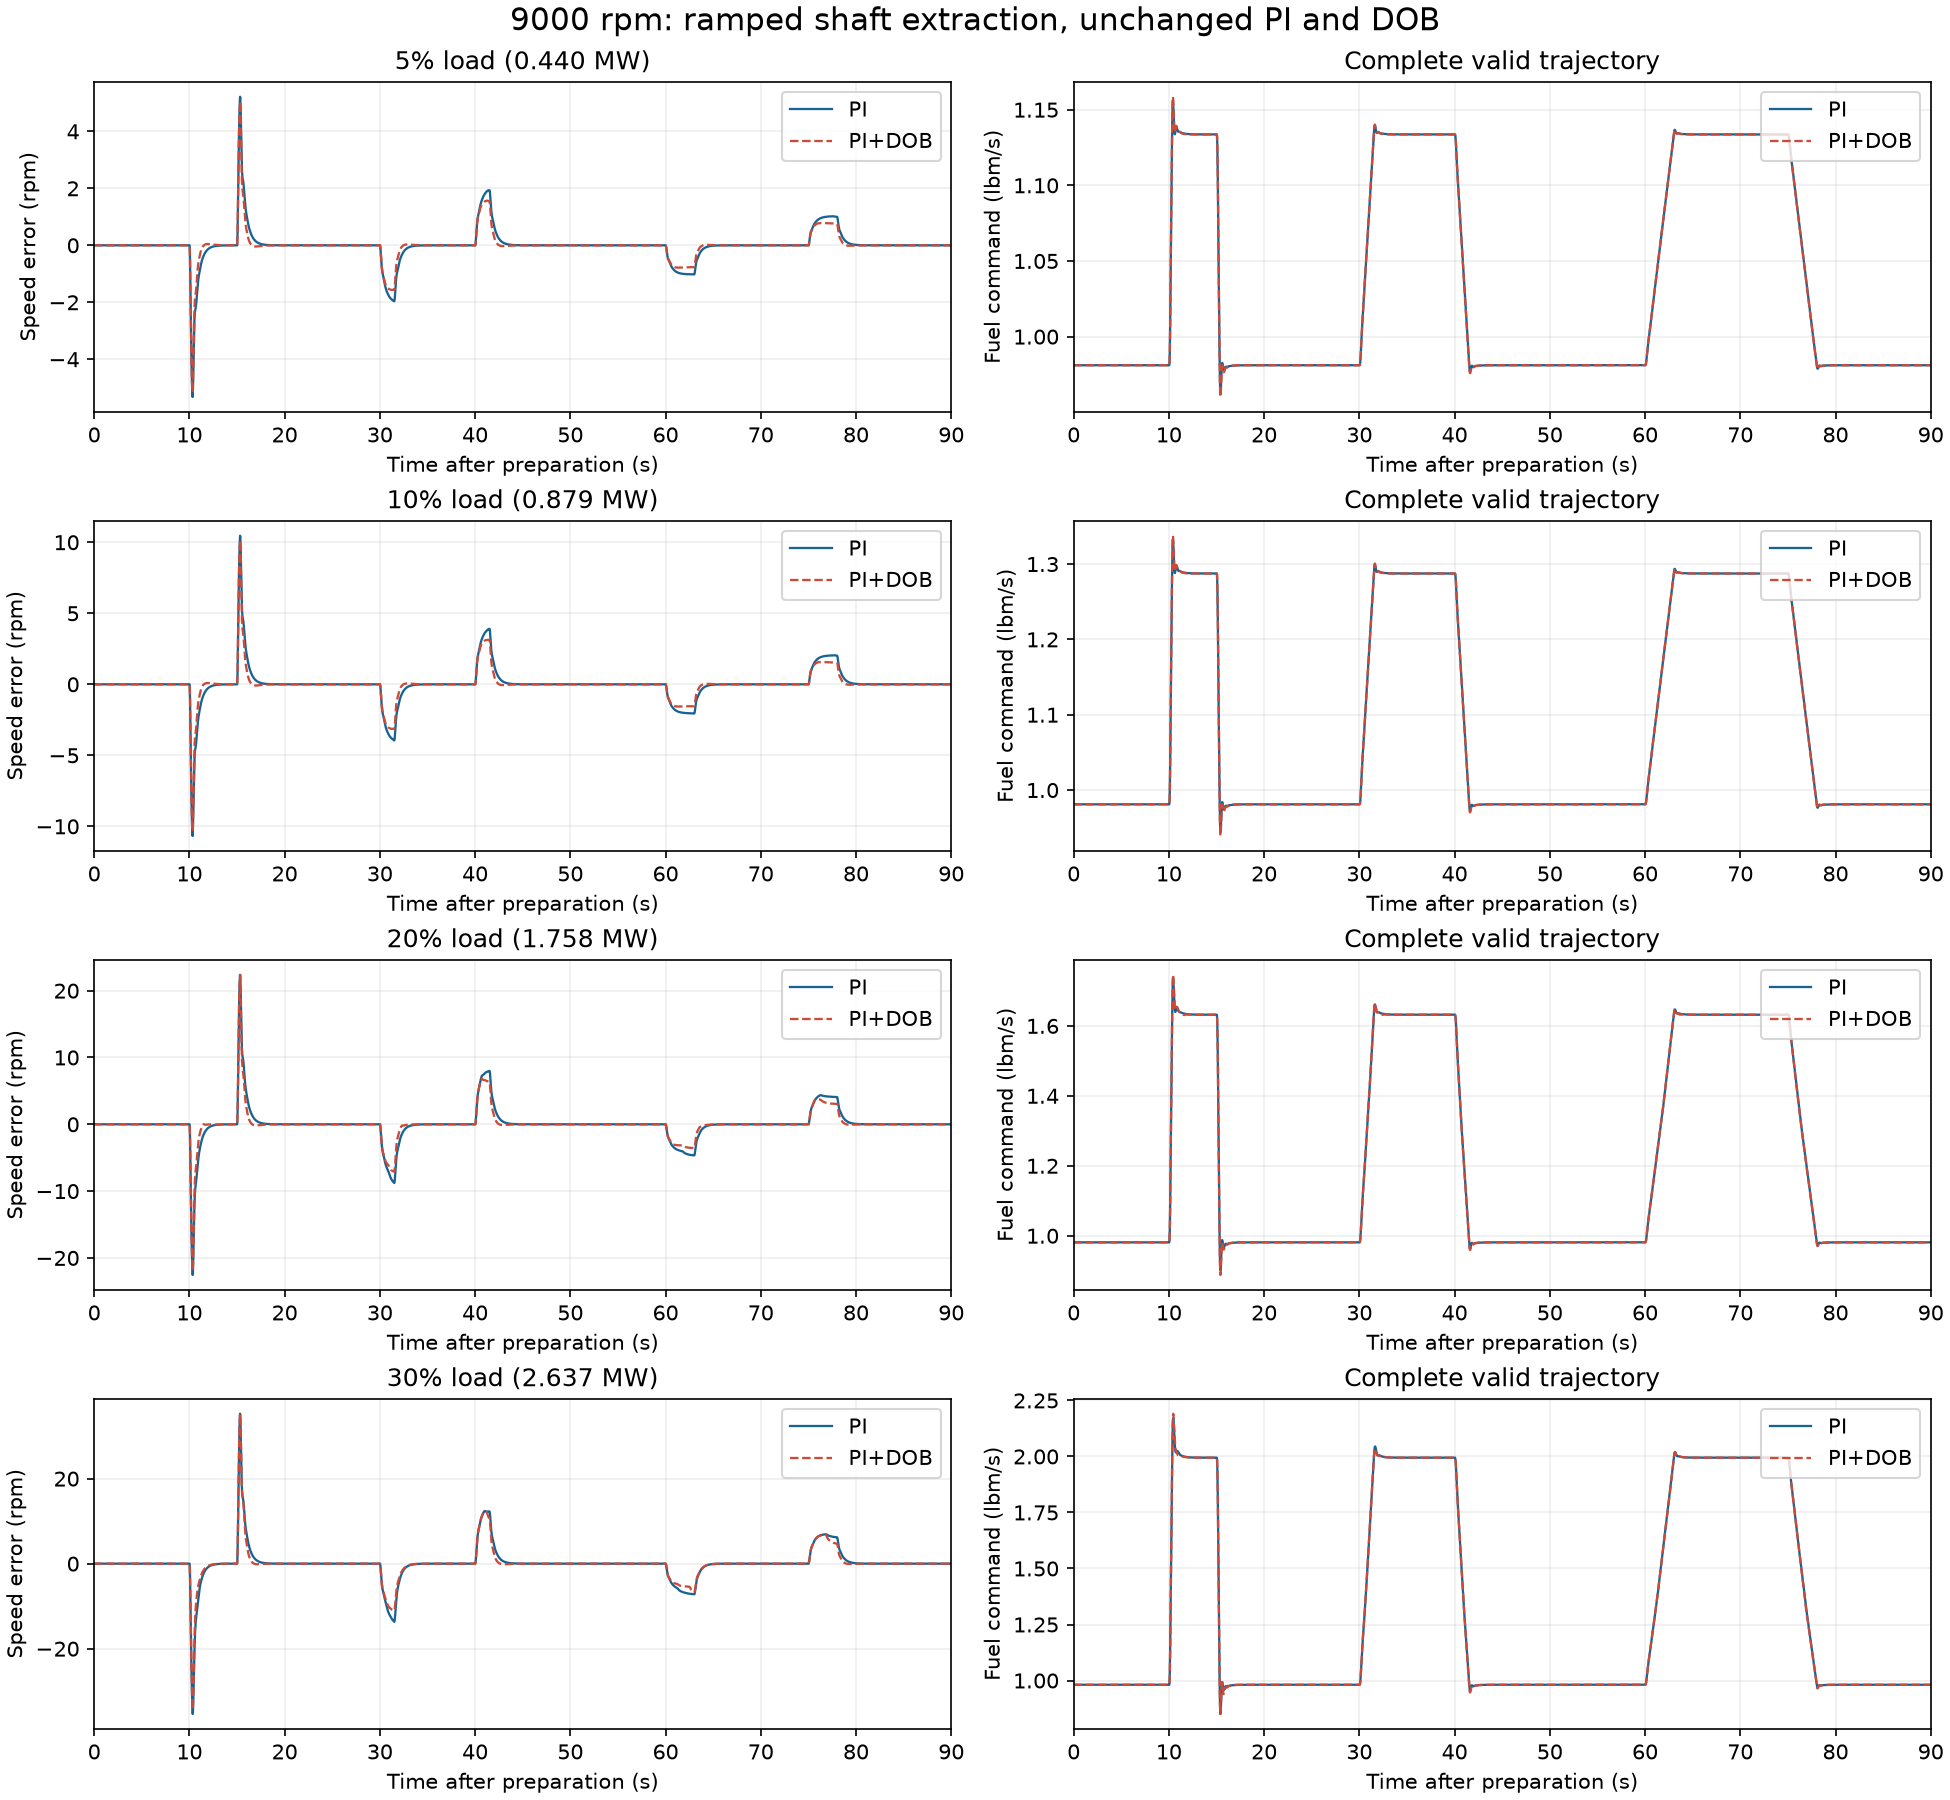
\includegraphics[width=.95\linewidth,height=.6\textheight,keepaspectratio]{early_PTO_9000rpm_ramp_comparison_overview.png}\caption{Overview. Archived study figure.}\end{figure}

\subsection{Time response at each ramp}

Recovery is the first sample after the last excursion outside $\pm$1 rpm, confirmed by at least 0.5 s within the band through the next ramp start. After-ramp recovery is max(0, recovery from start - ramp duration). A zero means recovery occurred by ramp completion. Metrics are withheld for an event if any earlier plant solve was invalid. A dash can also mean no confirmed settling.

{\scriptsize\setlength{\tabcolsep}{1.5mm}\begin{longtable}{>{\raggedright\arraybackslash}p{19.86mm}>{\raggedright\arraybackslash}p{19.86mm}>{\raggedright\arraybackslash}p{19.86mm}>{\raggedright\arraybackslash}p{19.86mm}>{\raggedright\arraybackslash}p{19.86mm}>{\raggedright\arraybackslash}p{19.86mm}>{\raggedright\arraybackslash}p{19.86mm}}\caption{The 9000-rpm ramped-load envelope: Time response at each ramp. Archived values.}\\\toprule
Load & Ramp s & Edge & Controller & Peak error rpm & Recovery from start s & After ramp s\\\midrule
\endfirsthead
Load & Ramp s & Edge & Controller & Peak error rpm & Recovery from start s & After ramp s\\\midrule
\endhead
5\% & 0.30 & application & PI & 5.325 & 1.035 & 0.735\\
5\% & 0.30 & removal & PI & 5.215 & 1.050 & 0.750\\
5\% & 1.50 & application & PI & 1.965 & 1.785 & 0.285\\
5\% & 1.50 & removal & PI & 1.932 & 1.785 & 0.285\\
5\% & 3.00 & application & PI & 1.020 & 3.045 & 0.045\\
5\% & 3.00 & removal & PI & 1.020 & 2.985 & 0.000\\
5\% & 0.30 & application & PI+DOB & 5.162 & 0.825 & 0.525\\
5\% & 0.30 & removal & PI+DOB & 5.055 & 0.825 & 0.525\\
5\% & 1.50 & application & PI+DOB & 1.565 & 1.665 & 0.165\\
5\% & 1.50 & removal & PI+DOB & 1.567 & 1.650 & 0.150\\
5\% & 3.00 & application & PI+DOB & 0.784 & 0.000 & 0.000\\
5\% & 3.00 & removal & PI+DOB & 0.782 & 0.000 & 0.000\\
10\% & 0.30 & application & PI & 10.677 & 1.350 & 1.050\\
10\% & 0.30 & removal & PI & 10.457 & 1.380 & 1.080\\
10\% & 1.50 & application & PI & 3.950 & 2.130 & 0.630\\
10\% & 1.50 & removal & PI & 3.901 & 2.145 & 0.645\\
10\% & 3.00 & application & PI & 2.054 & 3.315 & 0.315\\
10\% & 3.00 & removal & PI & 2.042 & 3.315 & 0.315\\
10\% & 0.30 & application & PI+DOB & 10.351 & 1.005 & 0.705\\
10\% & 0.30 & removal & PI+DOB & 10.140 & 1.035 & 0.735\\
10\% & 1.50 & application & PI+DOB & 3.145 & 1.845 & 0.345\\
10\% & 1.50 & removal & PI+DOB & 3.134 & 1.860 & 0.360\\
10\% & 3.00 & application & PI+DOB & 1.565 & 3.165 & 0.165\\
10\% & 3.00 & removal & PI+DOB & 1.566 & 3.150 & 0.150\\
20\% & 0.30 & application & PI & 22.553 & 1.695 & 1.395\\
20\% & 0.30 & removal & PI & 22.380 & 1.740 & 1.440\\
20\% & 1.50 & application & PI & 8.786 & 2.490 & 0.990\\
20\% & 1.50 & removal & PI & 7.988 & 2.490 & 0.990\\
20\% & 3.00 & application & PI & 4.649 & 3.705 & 0.705\\
20\% & 3.00 & removal & PI & 4.363 & 3.660 & 0.660\\
20\% & 0.30 & application & PI+DOB & 21.914 & 1.170 & 0.870\\
20\% & 0.30 & removal & PI+DOB & 22.329 & 1.215 & 0.915\\
20\% & 1.50 & application & PI+DOB & 7.096 & 2.055 & 0.555\\
20\% & 1.50 & removal & PI+DOB & 6.823 & 2.040 & 0.540\\
20\% & 3.00 & application & PI+DOB & 3.536 & 3.360 & 0.360\\
20\% & 3.00 & removal & PI+DOB & 3.771 & 3.345 & 0.345\\
30\% & 0.30 & application & PI & 35.359 & 1.875 & 1.575\\
30\% & 0.30 & removal & PI & 35.257 & 1.950 & 1.650\\
30\% & 1.50 & application & PI & 13.677 & 2.685 & 1.185\\
30\% & 1.50 & removal & PI & 12.372 & 2.700 & 1.200\\
30\% & 3.00 & application & PI & 7.239 & 3.900 & 0.900\\
30\% & 3.00 & removal & PI & 6.909 & 3.870 & 0.870\\
30\% & 0.30 & application & PI+DOB & 34.333 & 1.680 & 1.380\\
30\% & 0.30 & removal & PI+DOB & 35.258 & 1.410 & 1.110\\
30\% & 1.50 & application & PI+DOB & 11.032 & 2.580 & 1.080\\
30\% & 1.50 & removal & PI+DOB & 12.372 & 2.190 & 0.690\\
30\% & 3.00 & application & PI+DOB & 6.730 & 3.870 & 0.870\\
30\% & 3.00 & removal & PI+DOB & 6.901 & 3.480 & 0.480\\
\bottomrule\end{longtable}}

\subsection{Ramp rates}

{\scriptsize\setlength{\tabcolsep}{1.5mm}\begin{longtable}{>{\raggedright\arraybackslash}p{37.00mm}>{\raggedright\arraybackslash}p{37.00mm}>{\raggedright\arraybackslash}p{37.00mm}>{\raggedright\arraybackslash}p{37.00mm}}\caption{The 9000-rpm ramped-load envelope: Ramp rates. Archived values.}\\\toprule
Load & 0.30 s ramp (MW/s) & 1.50 s ramp (MW/s) & 3.00 s ramp (MW/s)\\\midrule
\endfirsthead
Load & 0.30 s ramp (MW/s) & 1.50 s ramp (MW/s) & 3.00 s ramp (MW/s)\\\midrule
\endhead
5\% & 1.465 & 0.293 & 0.147\\
10\% & 2.930 & 0.586 & 0.293\\
20\% & 5.861 & 1.172 & 0.586\\
30\% & 8.791 & 1.758 & 0.879\\
\bottomrule\end{longtable}}

These magnitudes apply to both rising and falling ramps. The source is sampled and held at 15 ms.

\subsection{Interpretation}

\par\noindent\textbullet\ \textbf{5\%:} observer RMSE changes by -13.03\% relative to PI. Peak absolute error changes from 5.325 to 5.162 rpm. Minimum compressor margin is 29.404\% / 29.347\% (PI / DOB). DOB compensation clips for 0.00\% of evaluation samples.
\par\noindent\textbullet\ \textbf{10\%:} observer RMSE changes by -13.02\% relative to PI. Peak absolute error changes from 10.677 to 10.351 rpm. Minimum compressor margin is 24.429\% / 24.322\% (PI / DOB). DOB compensation clips for 0.00\% of evaluation samples.
\par\noindent\textbullet\ \textbf{20\%:} observer RMSE changes by -11.92\% relative to PI. Peak absolute error changes from 22.553 to 22.329 rpm. Minimum compressor margin is 14.445\% / 14.238\% (PI / DOB). DOB compensation clips for 26.98\% of evaluation samples.
\par\noindent\textbullet\ \textbf{30\%:} observer RMSE changes by -7.77\% relative to PI. Peak absolute error changes from 35.359 to 35.258 rpm. Minimum compressor margin is 5.526\% / 5.231\% (PI / DOB). DOB compensation clips for 31.98\% of evaluation samples.

At 30\% load, increasing the application ramp from 0.30 to 3.00 s reduces PI peak error from 35.359 to 7.239 rpm and DOB peak error from 34.333 to 6.730 rpm. However, on the 3.00 s application ramp the observer improves recovery after completion by only 0.030 s (0.900 to 0.870 s). On the 0.30 s removal ramp, the peak is effectively unchanged (35.257 versus 35.258 rpm), while after-ramp recovery improves from 1.650 to 1.110 s. This supports a recovery benefit, not uniform peak suppression. At 5\% with a 3.00 s ramp, DOB error stays within $\pm$1 rpm throughout both events.

All eight trajectories pass the numerical checks, with no fuel saturation. At 30\%, DOB peak fuel is 2.191 lbm/s and minimum reported compressor margin is 5.231\%. The lower margin and frequent compensation clipping motivate constraint-aware tuning before extending the load envelope. Compared with the earlier 9500 rpm step tests, both the operating point, absolute load and disturbance shape have changed: 30\% is now 2.637 MW rather than 4.286 MW. The valid result cannot be attributed solely to observer performance or solely to ramp shaping.

The DOB is bounded equivalent-input compensation around the existing PI loop. It estimates the combined effect of external load and nominal-model mismatch; its estimate is not a calibrated shaft-power measurement. Slower ramps generally give the controller more time to compensate, but the event table is the evidence for this plant: peak rejection, settling and global RMSE need not improve together. The three ramp rates share a trajectory with different preceding histories and hold lengths, so these are representative scenarios rather than independent rate-identification experiments.

The fixed model was identified from fuel-to-acceleration data and corrected for zero equilibrium acceleration before observer synthesis. Its inverse and low-pass filtering introduce a bandwidth tradeoff: stronger/faster compensation can improve rejection while amplifying sensor noise and model error. Compensation clipping limits authority. PI integral action provides steady regulation; no anti-windup was added for these comparisons.

Next steps are independent runs for each rate with identical settling windows, gain scheduling across operating points, sensor-noise and delay tests, anti-windup and explicit fuel, temperature, and compressor-margin constraints, then fixed-step embedded timing and hardware-in-the-loop assessment. If flow convergence fails, first establish a numerically valid operating envelope; an invalid trajectory is not proof of physical instability or surge.

\subsection{Verification and reproduction}

The two controllers receive identical sampled power profiles, verified against the ramp formula. Each run has 10001 samples through 150 s. The mechanical torque balance is reconstructed from logged turbine, compressor and external powers and checked against shaft acceleration. Validity requires finite signals, positive fuel and compressor margin, flow residual $\le$1e-9 and fewer than 200 solver iterations. All plots show only the prefix before the first invalid solve. Full raw trajectories are retained for diagnosis.

Run \path|run_tmats_pto_9000_ramp_batch| in MATLAB, then \path|summarize_pto_9000_ramps.py| in Python for the report. A single level is \texttt{out=run\_\allowbreak tmats\_\allowbreak pto\_\allowbreak study(0.10,9000,[0.30} \texttt{1.50} \texttt{3.00]);}. Omitting the third argument preserves the earlier step-load study. The existing PTO Simulink model is unchanged.

\subsection{5\% response zooms}

\begin{figure}[H]\centering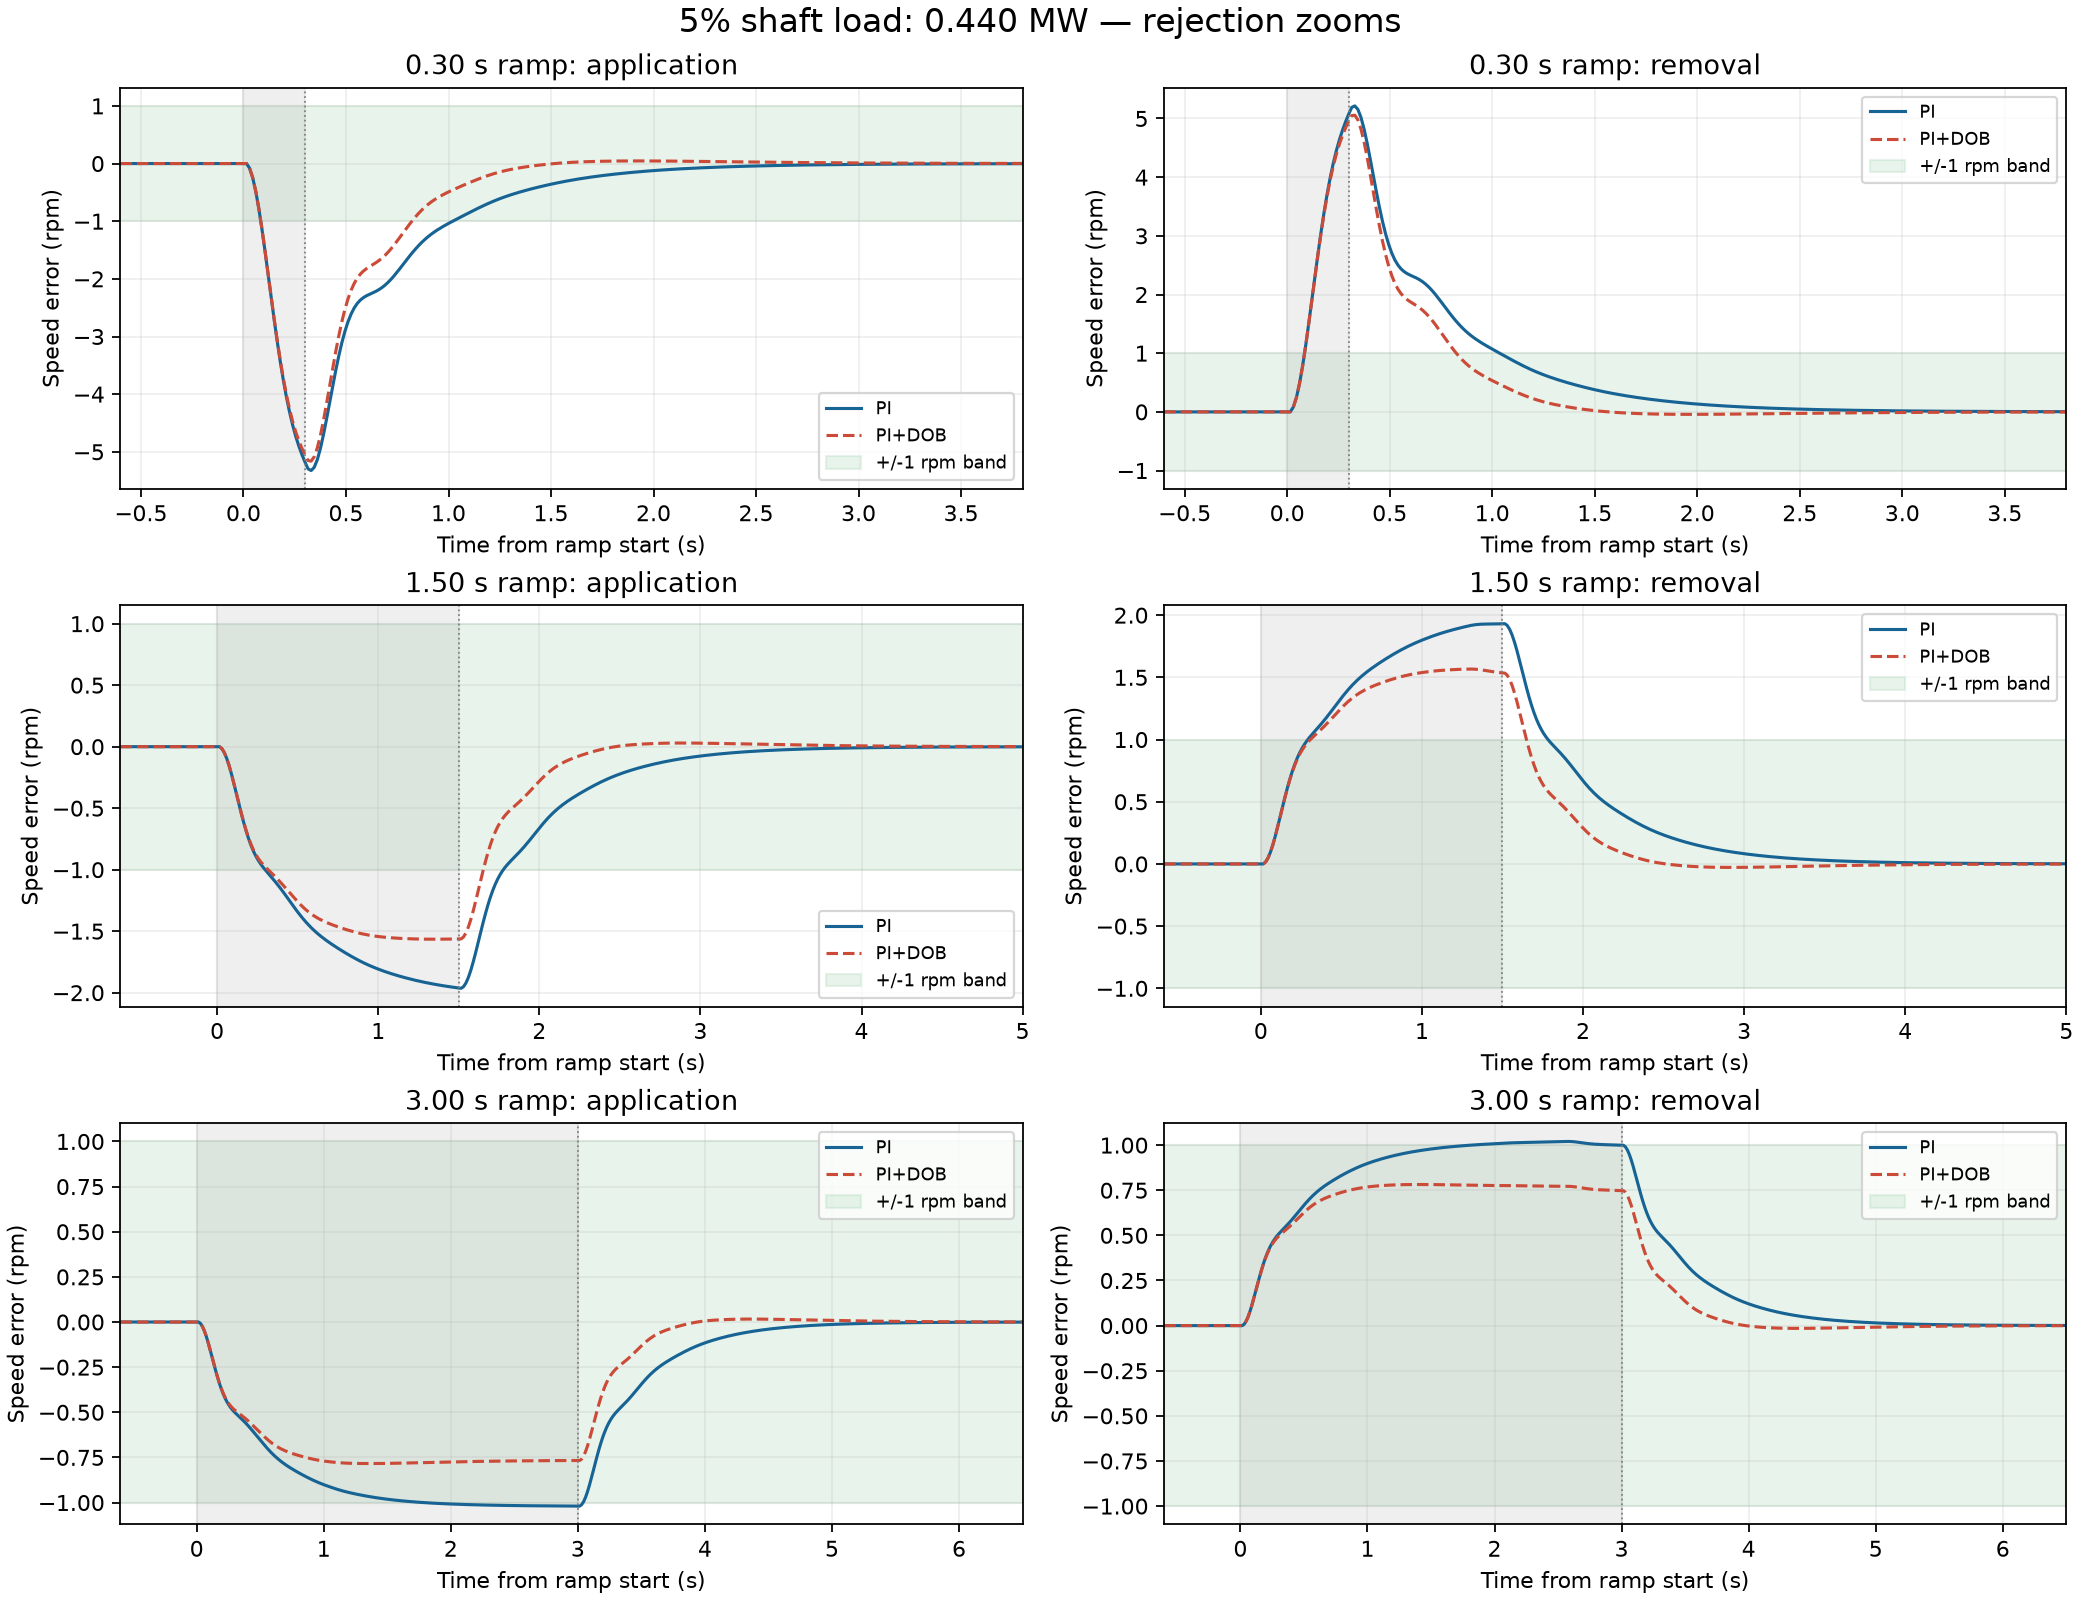
\includegraphics[width=.95\linewidth,height=.6\textheight,keepaspectratio]{early_PTO_9000rpm_ramp_comparison_zoom_05pct.png}\caption{5\% zoom. Archived study figure.}\end{figure}

\subsection{10\% response zooms}

\begin{figure}[H]\centering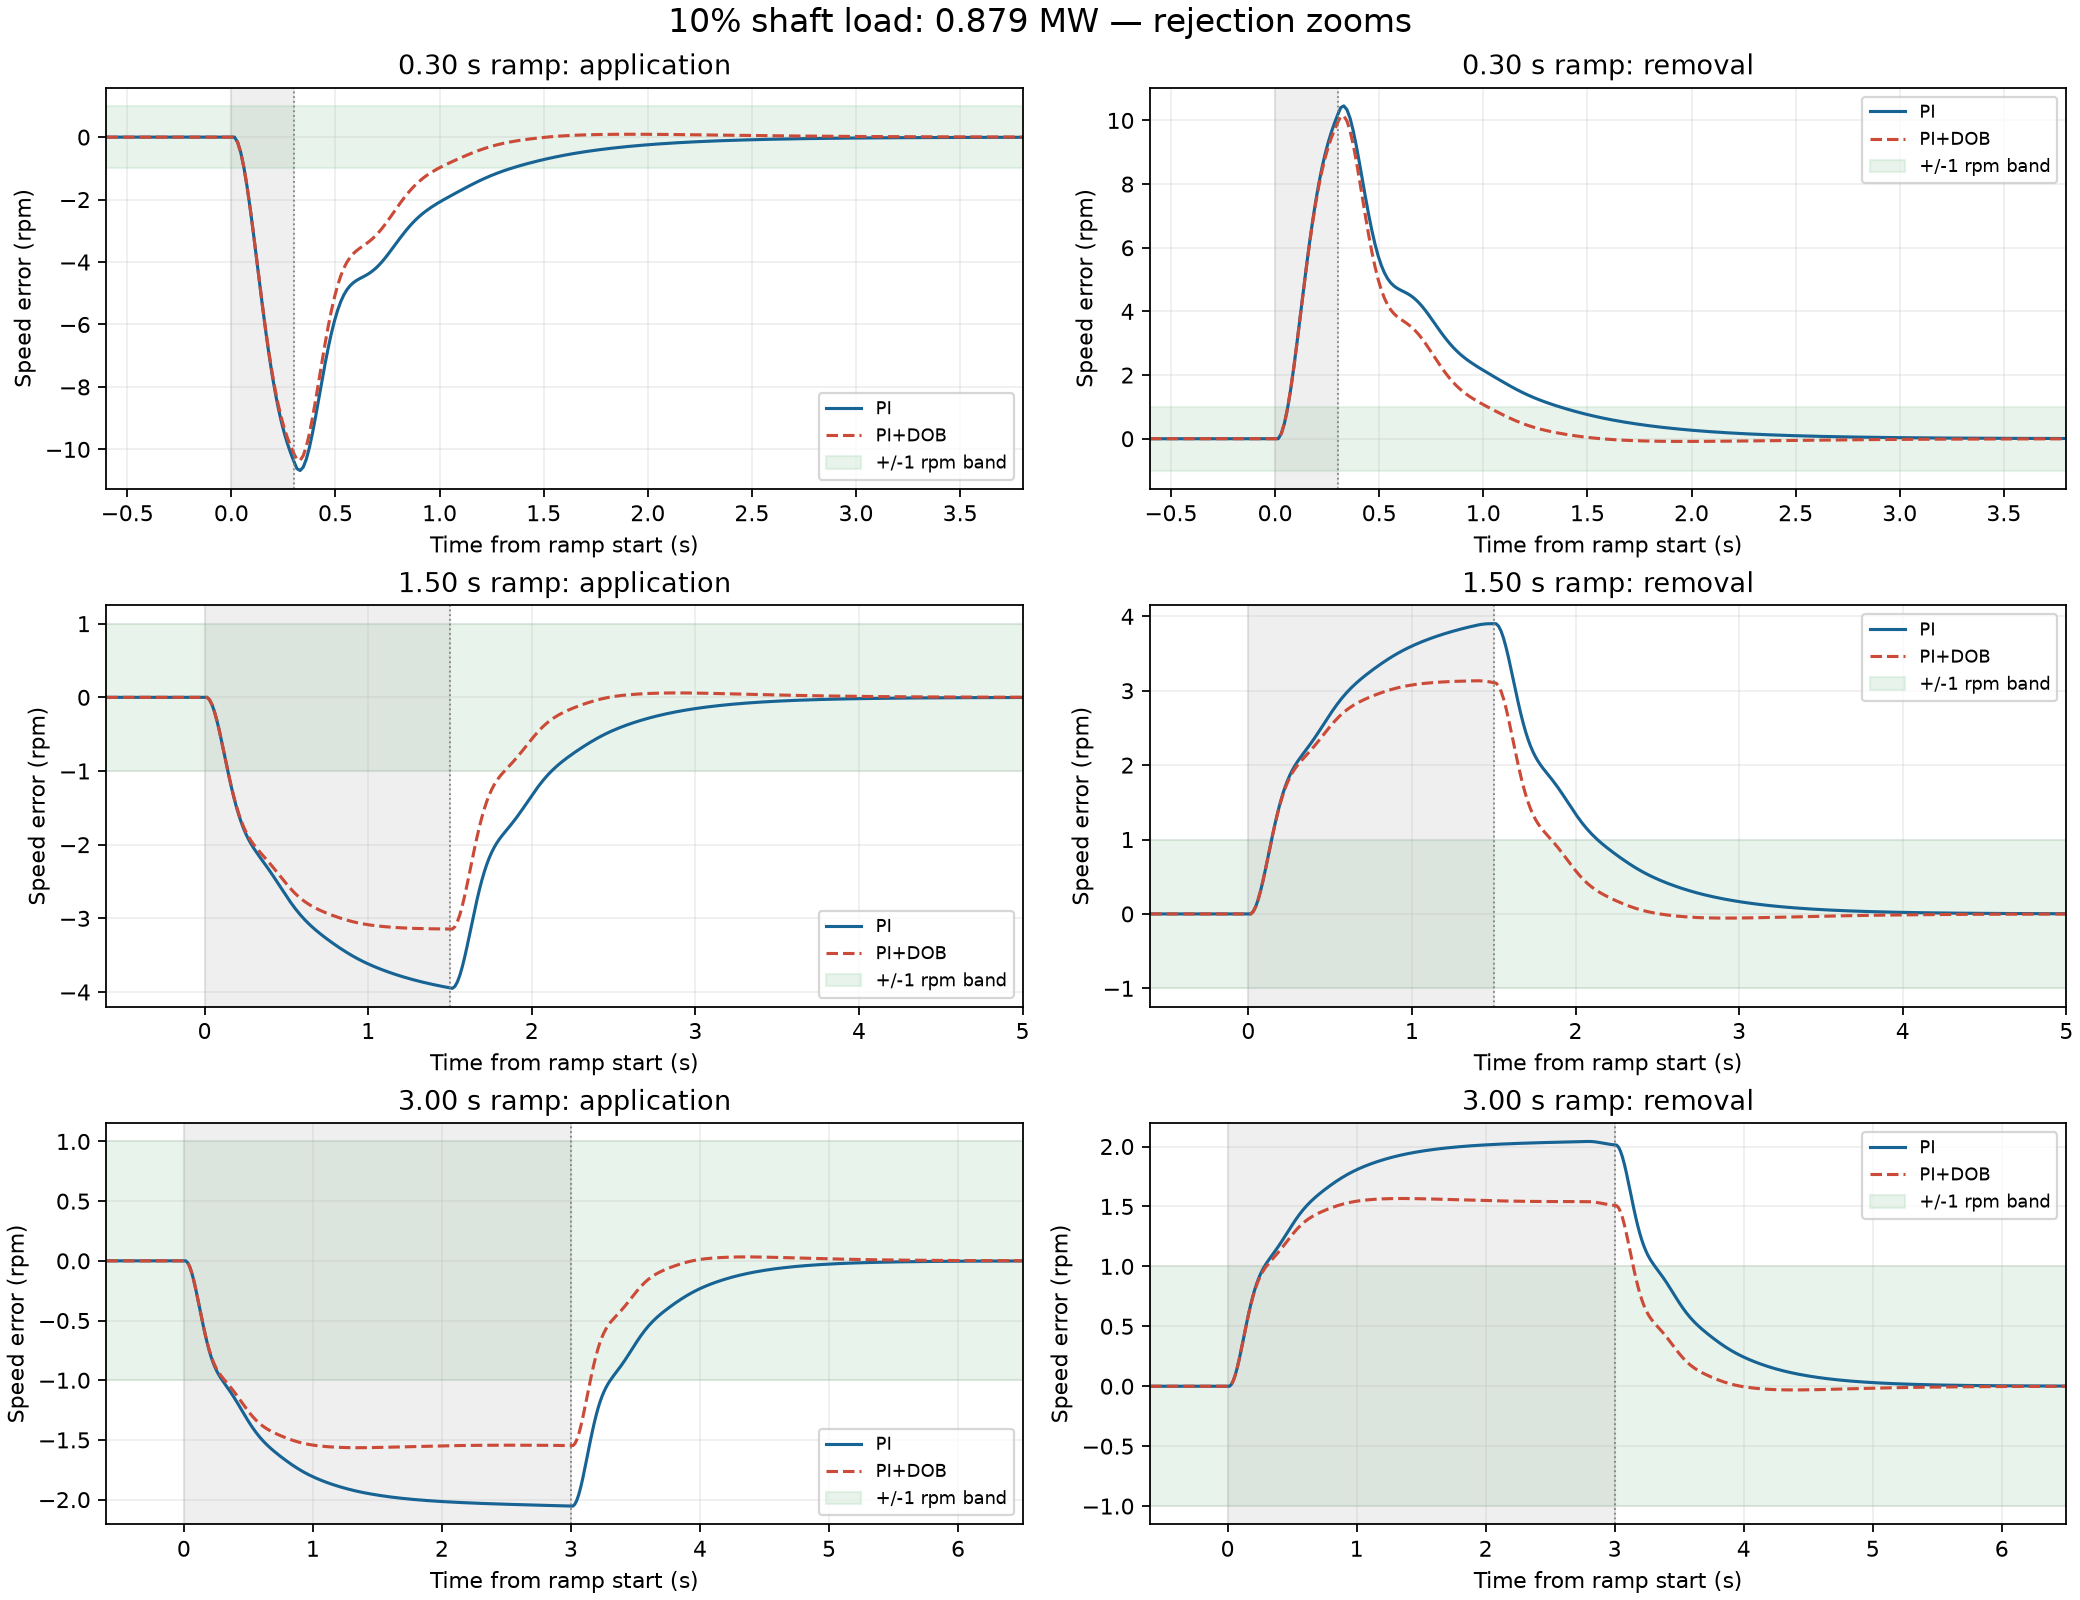
\includegraphics[width=.95\linewidth,height=.6\textheight,keepaspectratio]{early_PTO_9000rpm_ramp_comparison_zoom_10pct.png}\caption{10\% zoom. Archived study figure.}\end{figure}

\subsection{20\% response zooms}

\begin{figure}[H]\centering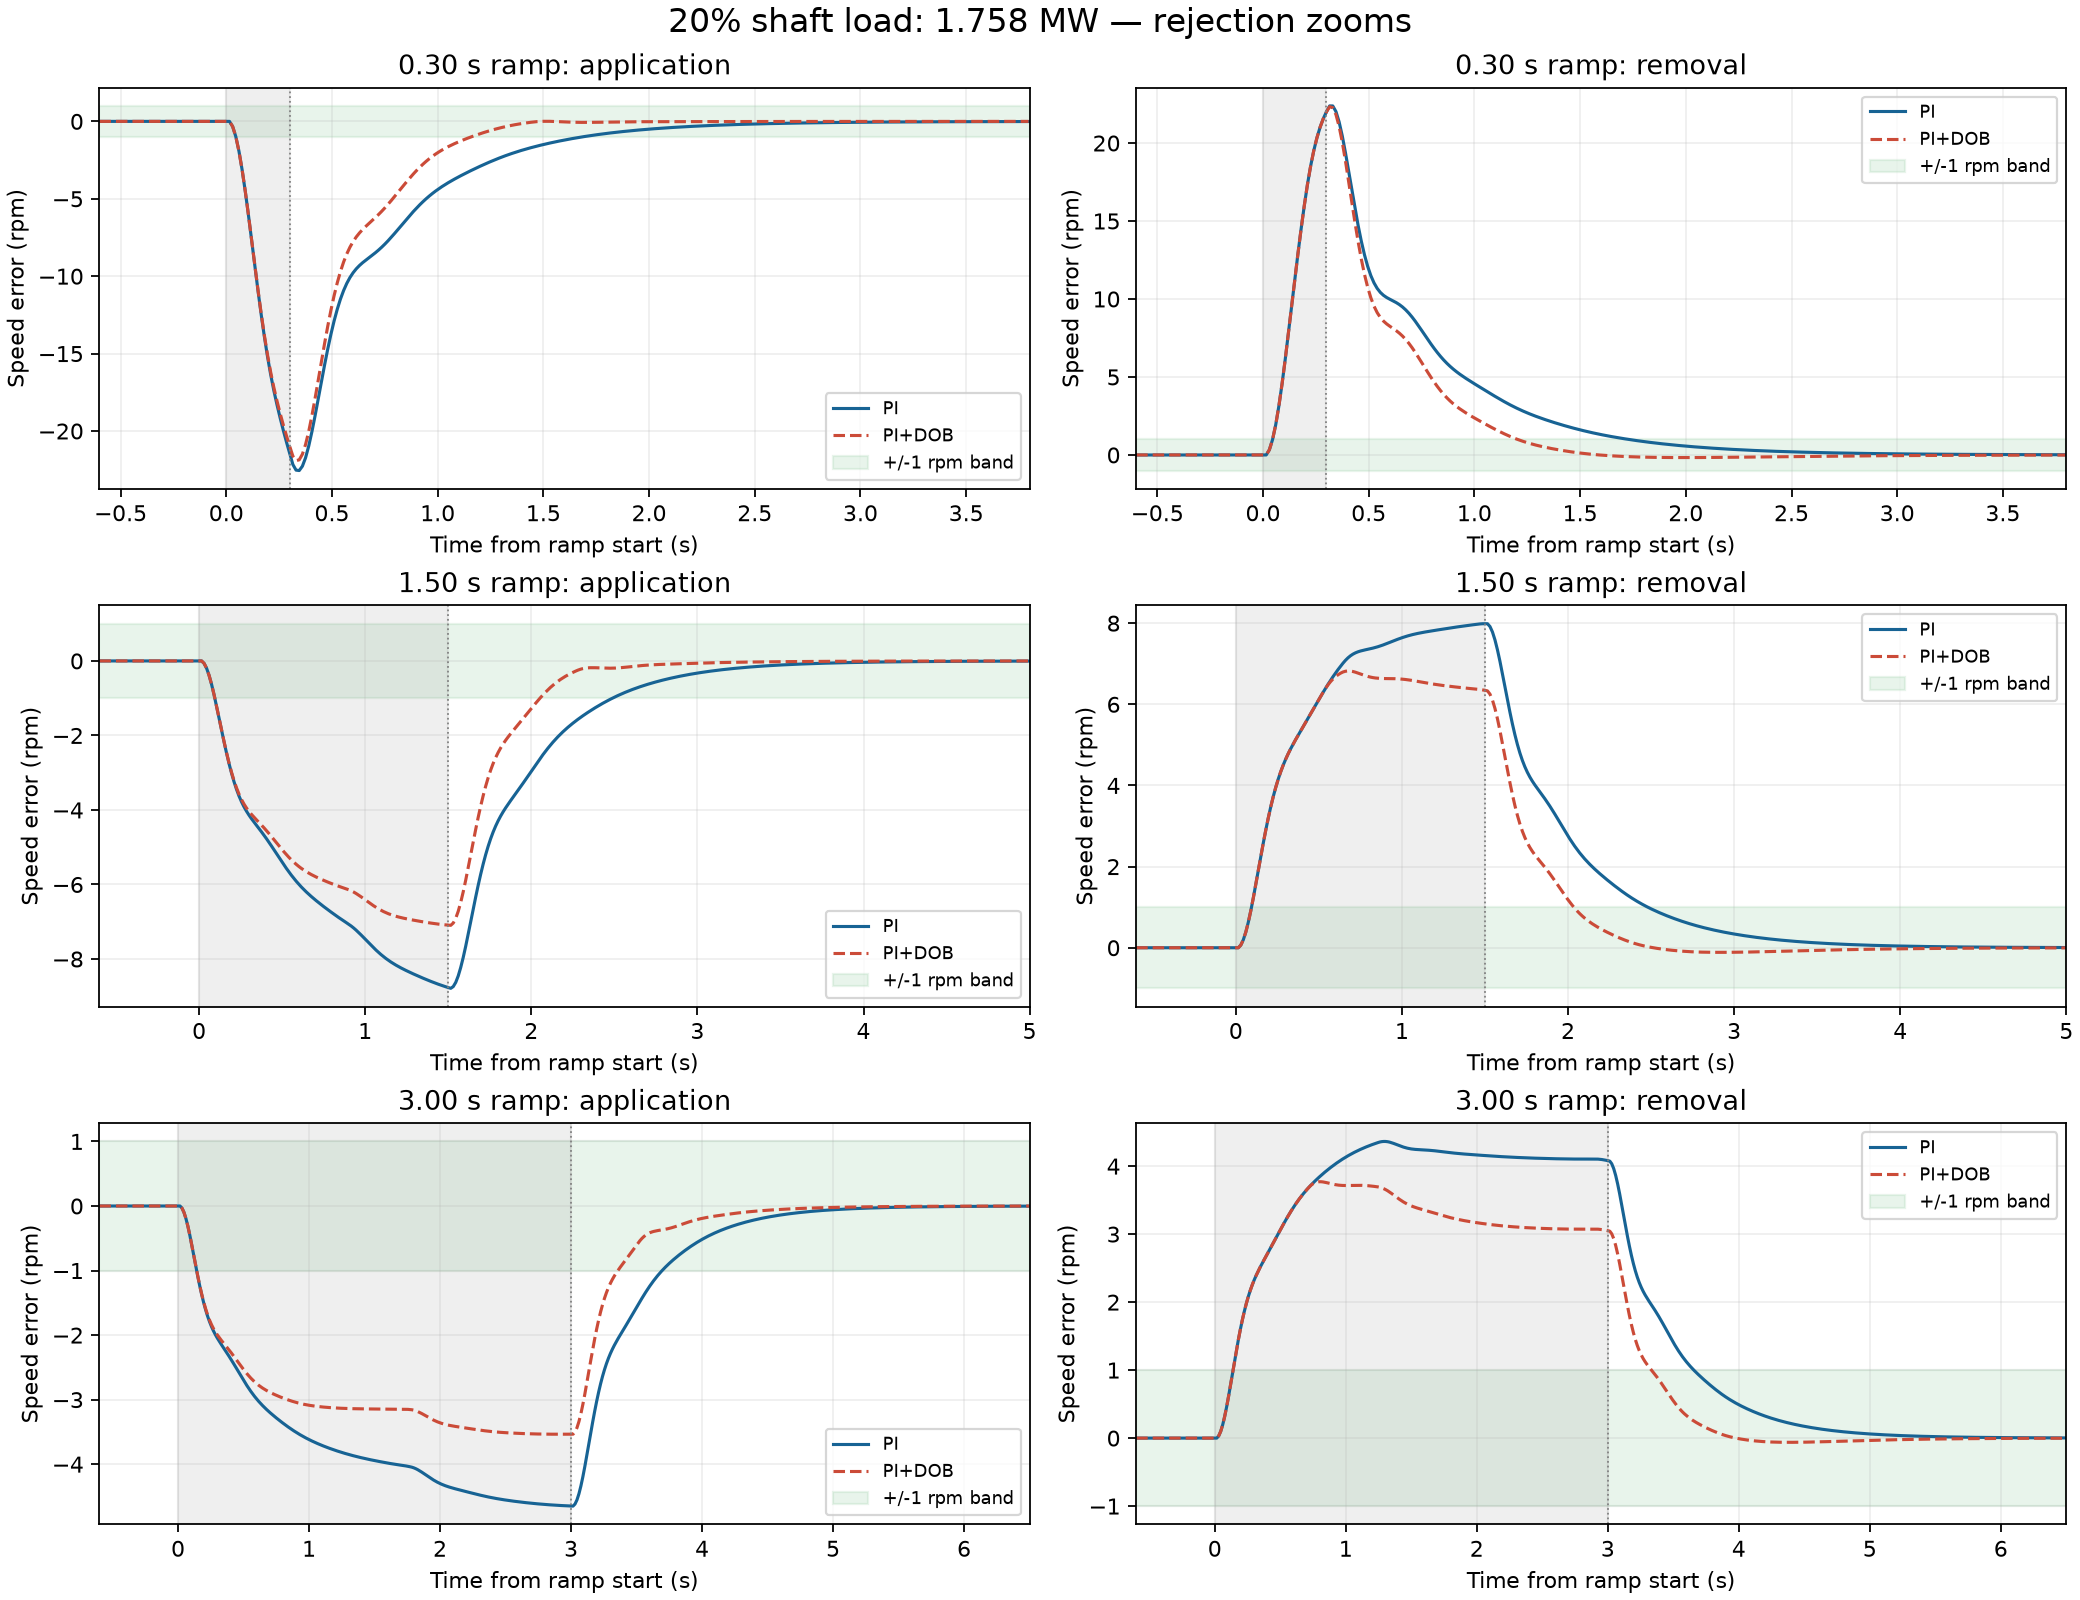
\includegraphics[width=.95\linewidth,height=.6\textheight,keepaspectratio]{early_PTO_9000rpm_ramp_comparison_zoom_20pct.png}\caption{20\% zoom. Archived study figure.}\end{figure}

\subsection{30\% response zooms}

\begin{figure}[H]\centering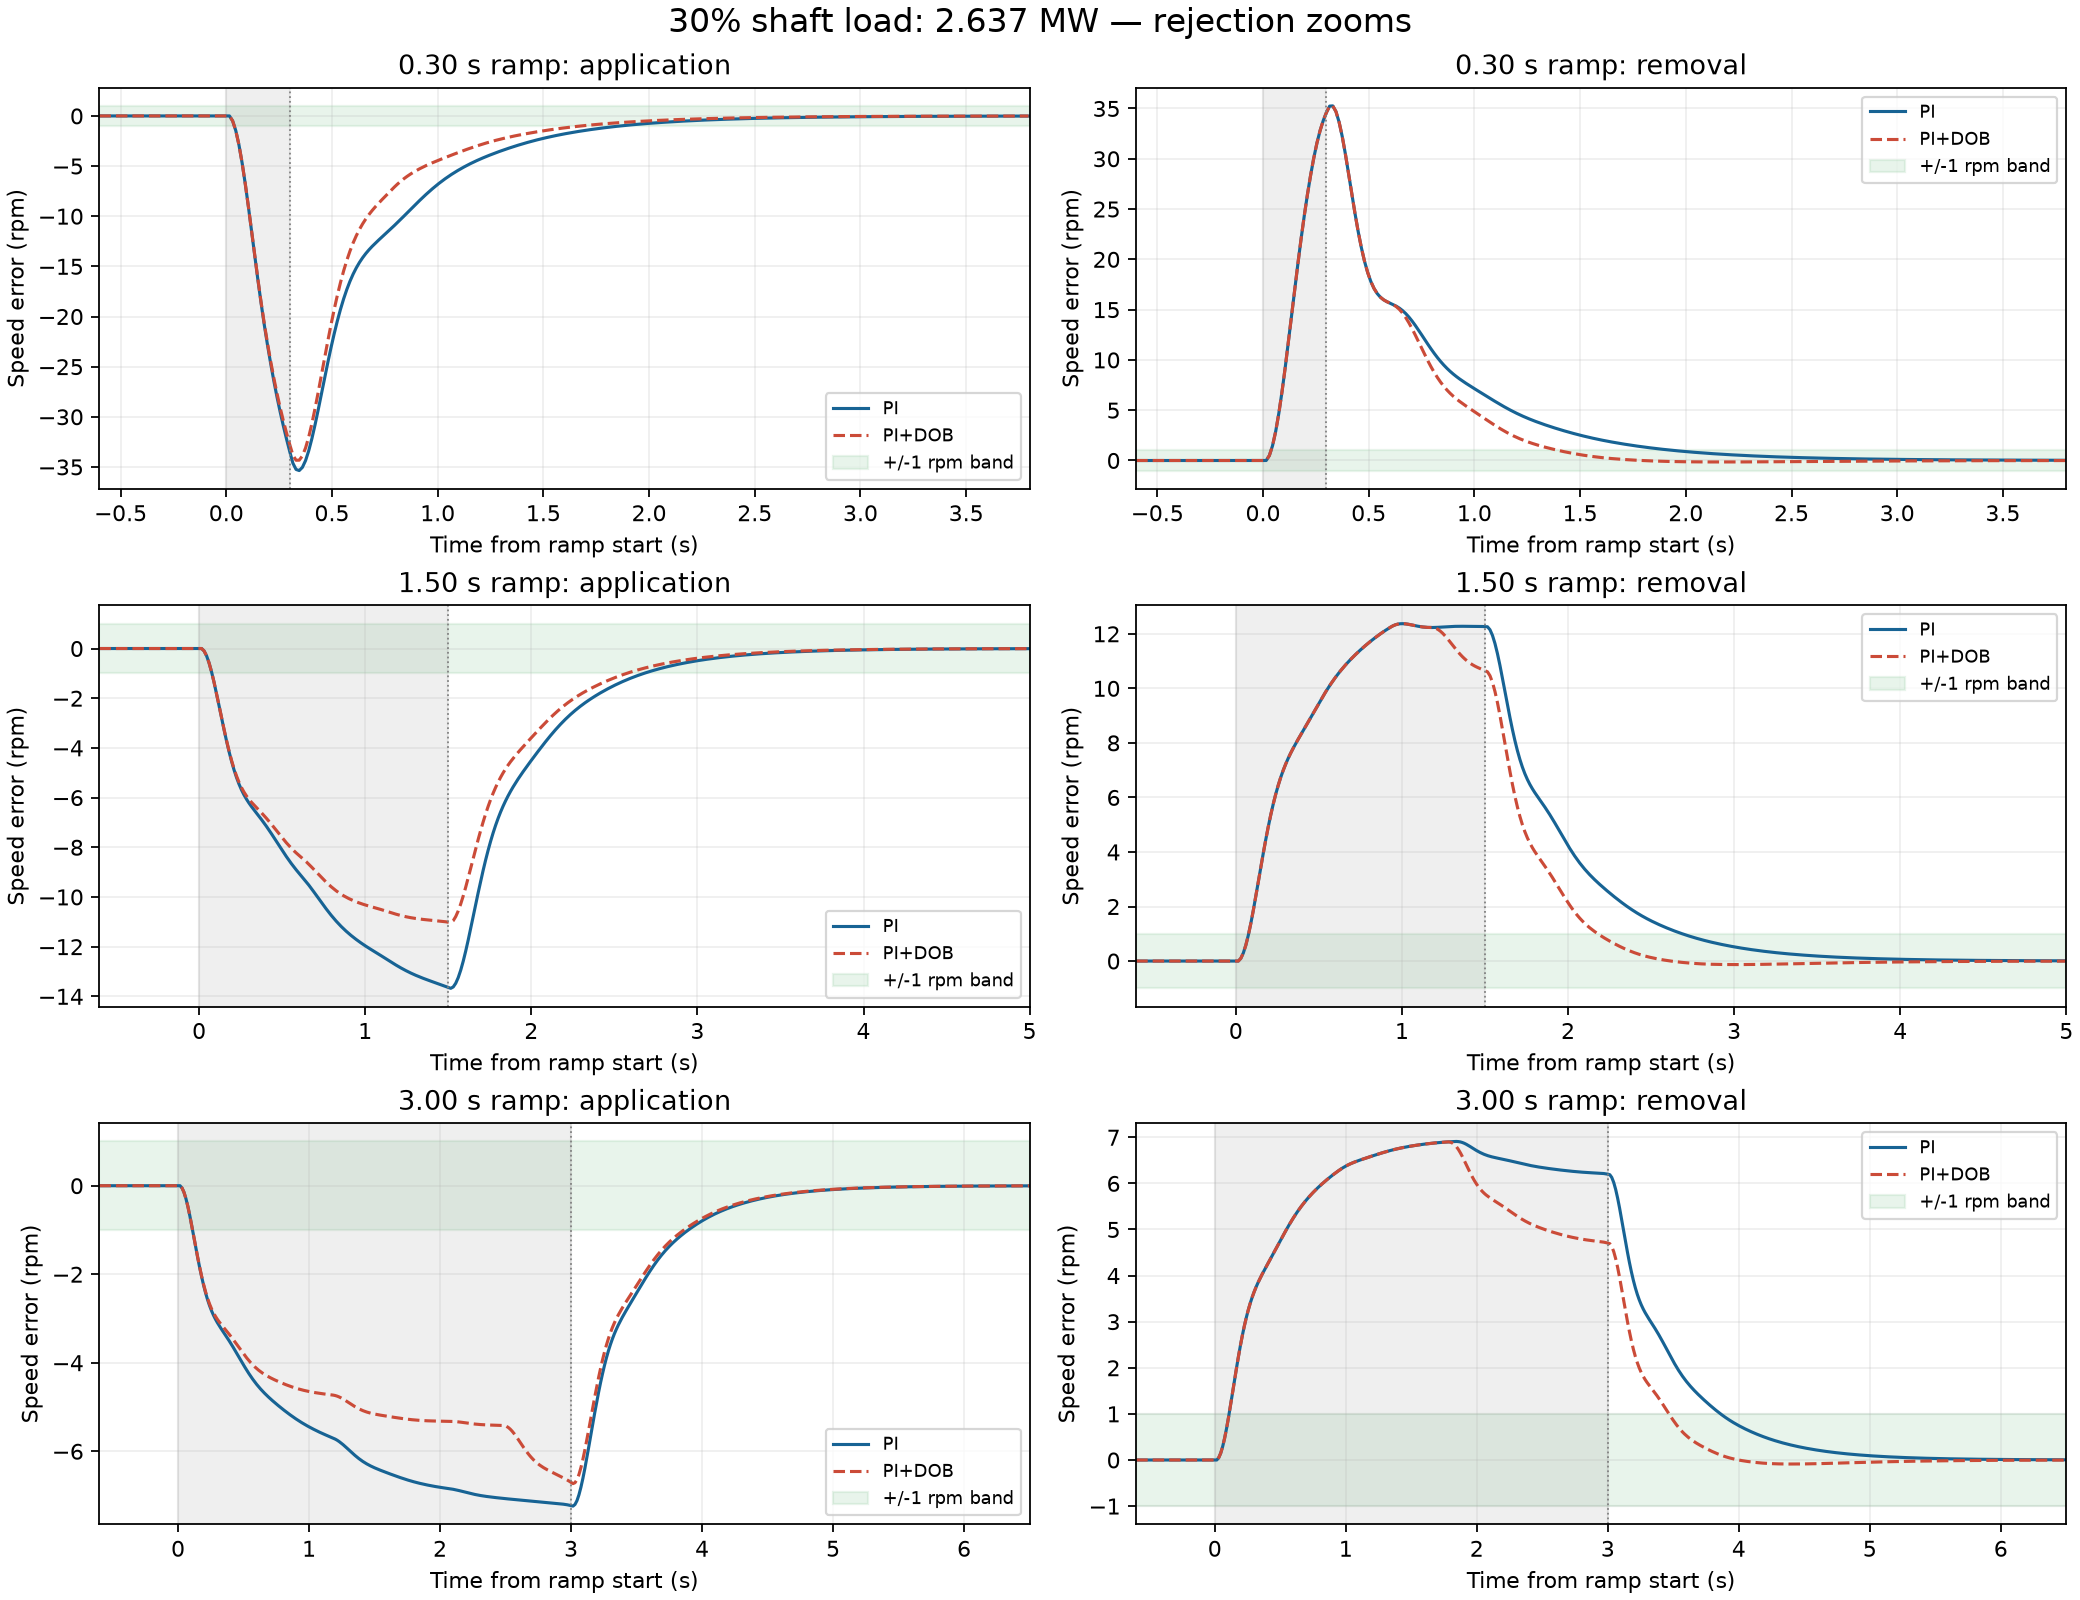
\includegraphics[width=.95\linewidth,height=.6\textheight,keepaspectratio]{early_PTO_9000rpm_ramp_comparison_zoom_30pct.png}\caption{30\% zoom. Archived study figure.}\end{figure}



\section{LESO, UDE, and GPIO implementation and first comparison}
\textit{Evidence basis: }\path|results/literature_observers_9000rpm_10pct_20260912_211600_355/REPORT.md|. The following detailed account is adapted from the archived study; references to simulation and verification describe historical work.\par

Load is \textbf{0.879124 MW} (10\% of 11789.245211 hp gross turbine power). The previous 0.30, 1.50 and 3.00 s ramp/hold/ramp scenario is repeated with five controllers. PI gains, 0.25 compensation gain, $\pm$0.15 lbm/s correction bound, fuel limits and preparation are unchanged. The observer pole-frequency parameter is 0.5 Hz for every method; actual estimator bandwidths differ. No test-based tuning is performed.

The three candidates are LESO (two states), UDE (one state), and ramp GPIO (three states). See the accompanying formulation for equations, primary literature, implementation details and comparison limitations.

\subsection{Measured comparison}

{\scriptsize\setlength{\tabcolsep}{1.5mm}\begin{longtable}{>{\raggedright\arraybackslash}p{19.86mm}>{\raggedright\arraybackslash}p{19.86mm}>{\raggedright\arraybackslash}p{19.86mm}>{\raggedright\arraybackslash}p{19.86mm}>{\raggedright\arraybackslash}p{19.86mm}>{\raggedright\arraybackslash}p{19.86mm}>{\raggedright\arraybackslash}p{19.86mm}}\caption{LESO, UDE, and GPIO implementation and first comparison: Measured comparison. Archived values.}\\\toprule
Method & Valid & RMSE rpm & Reduction vs PI & Peak error rpm & IAE rpm$\cdot$s & Peak fuel lbm/s\\\midrule
\endfirsthead
Method & Valid & RMSE rpm & Reduction vs PI & Peak error rpm & IAE rpm$\cdot$s & Peak fuel lbm/s\\\midrule
\endhead
PI & True & 1.193 & 0.000\% & 10.677 & 36.774 & 1.333\\
DOB & True & 1.038 & 13.021\% & 10.351 & 28.341 & 1.338\\
LESO & True & 1.039 & 12.903\% & 10.349 & 28.694 & 1.338\\
UDE & True & 0.969 & 18.746\% & 9.377 & 27.587 & 1.336\\
GPIO & True & 0.951 & 20.301\% & 9.866 & 27.577 & 1.344\\
\bottomrule\end{longtable}}

\begin{figure}[H]\centering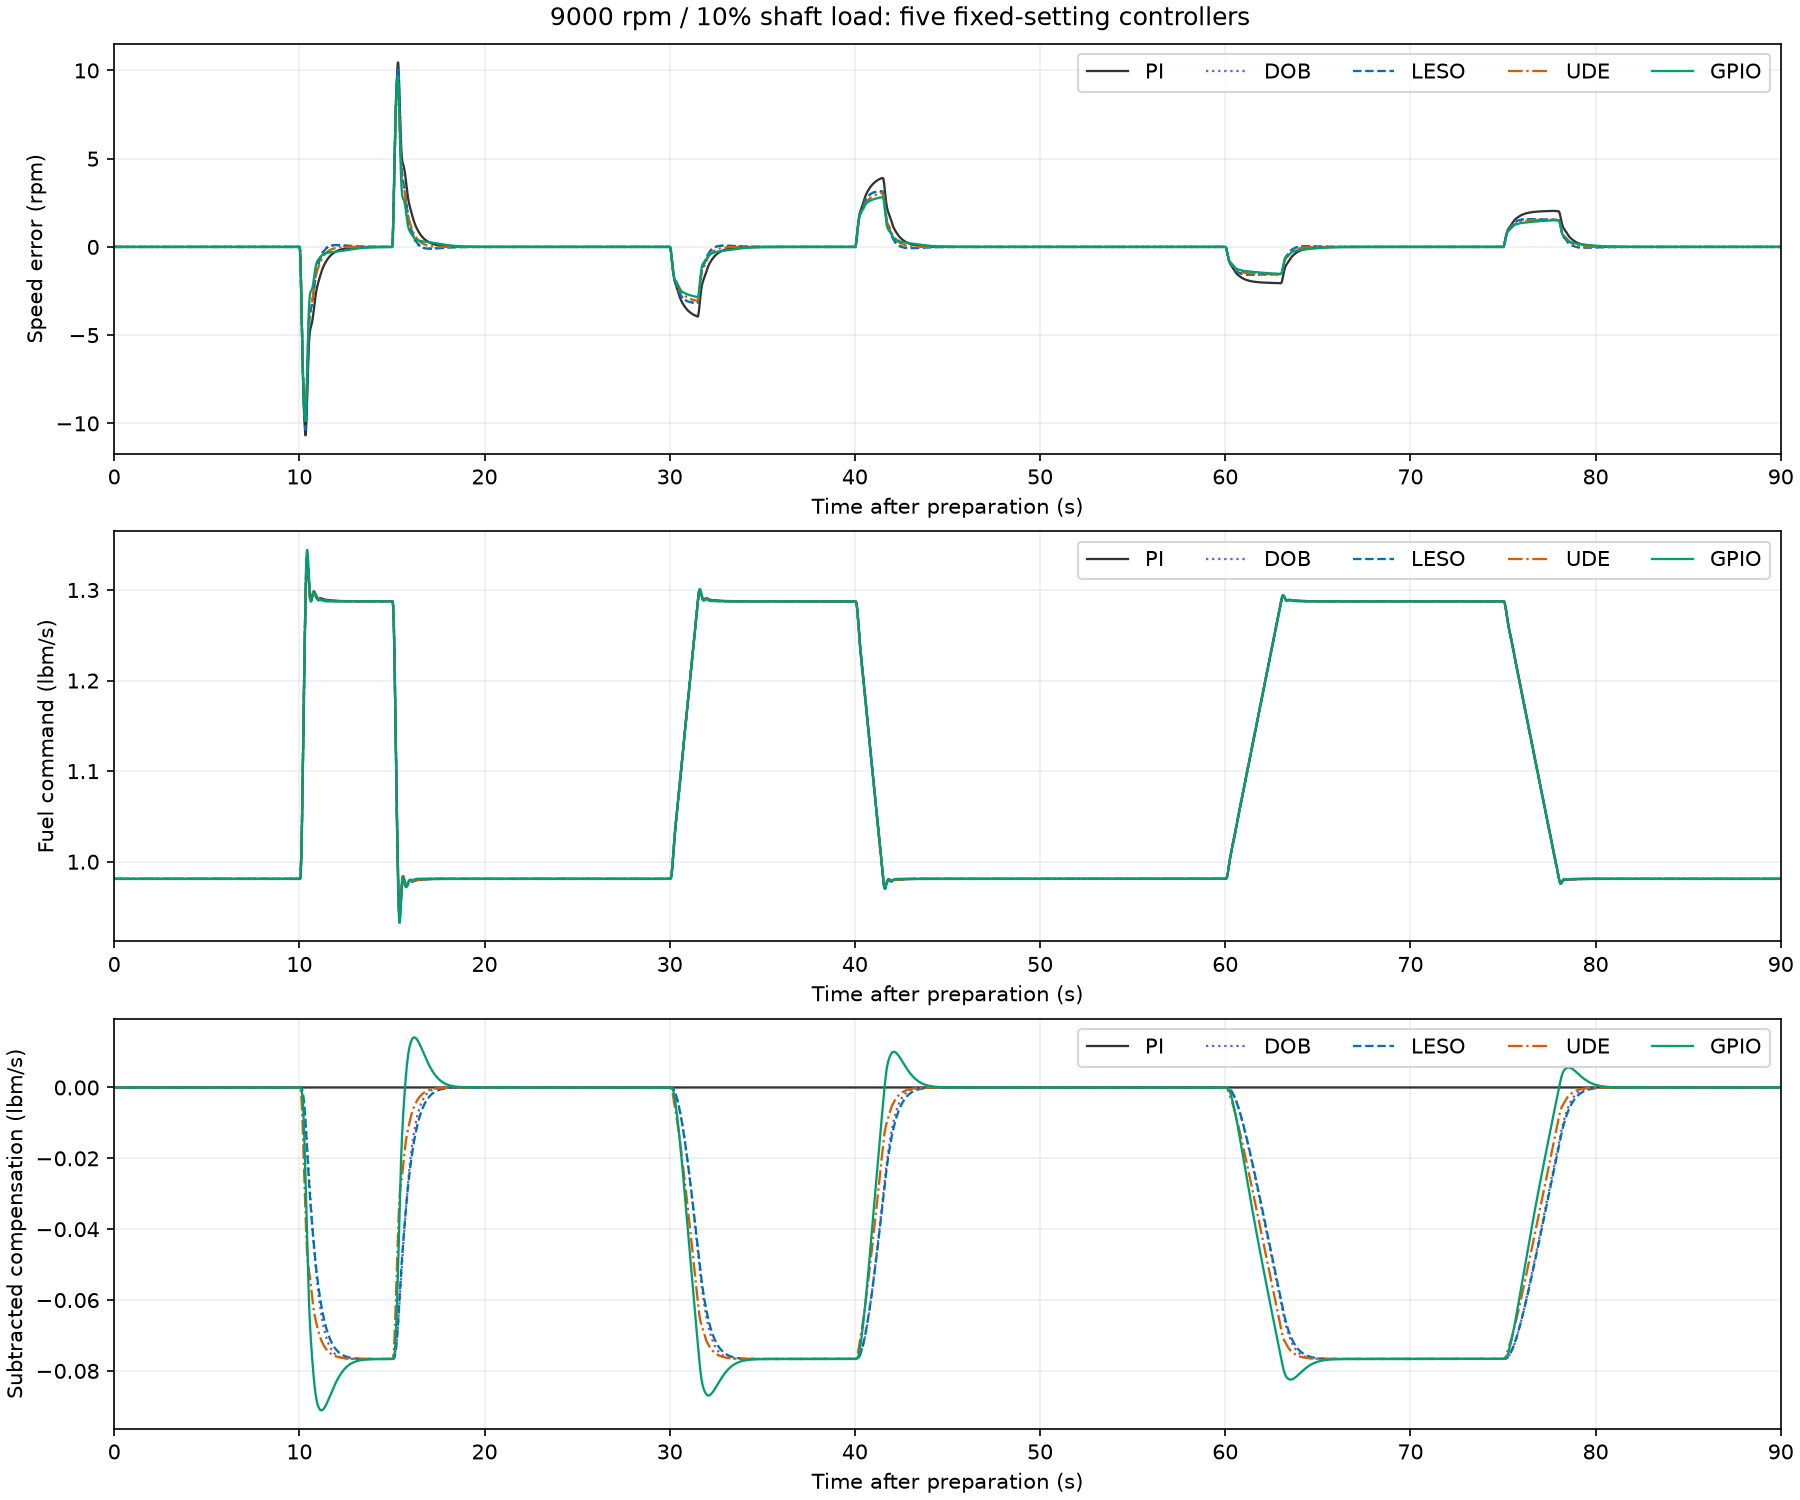
\includegraphics[width=.95\linewidth,height=.6\textheight,keepaspectratio]{early_literature_observers_9000rpm_10pct_20260912_211600_355_overview.png}\caption{Overview. Archived study figure.}\end{figure}

\subsection{Event recovery}

Recovery requires remaining within $\pm$1 rpm to the next ramp, with at least 0.5 s confirmed dwell. After-ramp recovery subtracts the ramp duration, bounded below by zero. Failed propagated trajectories receive no performance claim.

{\scriptsize\setlength{\tabcolsep}{1.5mm}\begin{longtable}{>{\raggedright\arraybackslash}p{23.67mm}>{\raggedright\arraybackslash}p{23.67mm}>{\raggedright\arraybackslash}p{23.67mm}>{\raggedright\arraybackslash}p{23.67mm}>{\raggedright\arraybackslash}p{23.67mm}>{\raggedright\arraybackslash}p{23.67mm}}\caption{LESO, UDE, and GPIO implementation and first comparison: Event recovery. Archived values.}\\\toprule
Ramp s & Edge & Method & Peak rpm & Recovery from start s & After ramp s\\\midrule
\endfirsthead
Ramp s & Edge & Method & Peak rpm & Recovery from start s & After ramp s\\\midrule
\endhead
0.30 & apply & PI & 10.677 & 1.350 & 1.050\\
0.30 & apply & DOB & 10.351 & 1.005 & 0.705\\
0.30 & apply & LESO & 10.349 & 1.020 & 0.720\\
0.30 & apply & UDE & 9.377 & 1.080 & 0.780\\
0.30 & apply & GPIO & 9.866 & 0.915 & 0.615\\
0.30 & remove & PI & 10.457 & 1.380 & 1.080\\
0.30 & remove & DOB & 10.140 & 1.035 & 0.735\\
0.30 & remove & LESO & 10.137 & 1.050 & 0.750\\
0.30 & remove & UDE & 9.205 & 1.095 & 0.795\\
0.30 & remove & GPIO & 9.670 & 0.930 & 0.630\\
1.50 & apply & PI & 3.950 & 2.130 & 0.630\\
1.50 & apply & DOB & 3.145 & 1.845 & 0.345\\
1.50 & apply & LESO & 3.171 & 1.845 & 0.345\\
1.50 & apply & UDE & 3.050 & 1.920 & 0.420\\
1.50 & apply & GPIO & 2.850 & 1.785 & 0.285\\
1.50 & remove & PI & 3.901 & 2.145 & 0.645\\
1.50 & remove & DOB & 3.134 & 1.860 & 0.360\\
1.50 & remove & LESO & 3.158 & 1.875 & 0.375\\
1.50 & remove & UDE & 3.022 & 1.920 & 0.420\\
1.50 & remove & GPIO & 2.817 & 1.800 & 0.300\\
3.00 & apply & PI & 2.054 & 3.315 & 0.315\\
3.00 & apply & DOB & 1.565 & 3.165 & 0.165\\
3.00 & apply & LESO & 1.577 & 3.165 & 0.165\\
3.00 & apply & UDE & 1.545 & 3.165 & 0.165\\
3.00 & apply & GPIO & 1.528 & 3.150 & 0.150\\
3.00 & remove & PI & 2.042 & 3.315 & 0.315\\
3.00 & remove & DOB & 1.566 & 3.150 & 0.150\\
3.00 & remove & LESO & 1.578 & 3.150 & 0.150\\
3.00 & remove & UDE & 1.536 & 3.150 & 0.150\\
3.00 & remove & GPIO & 1.513 & 3.150 & 0.150\\
\bottomrule\end{longtable}}

\begin{figure}[H]\centering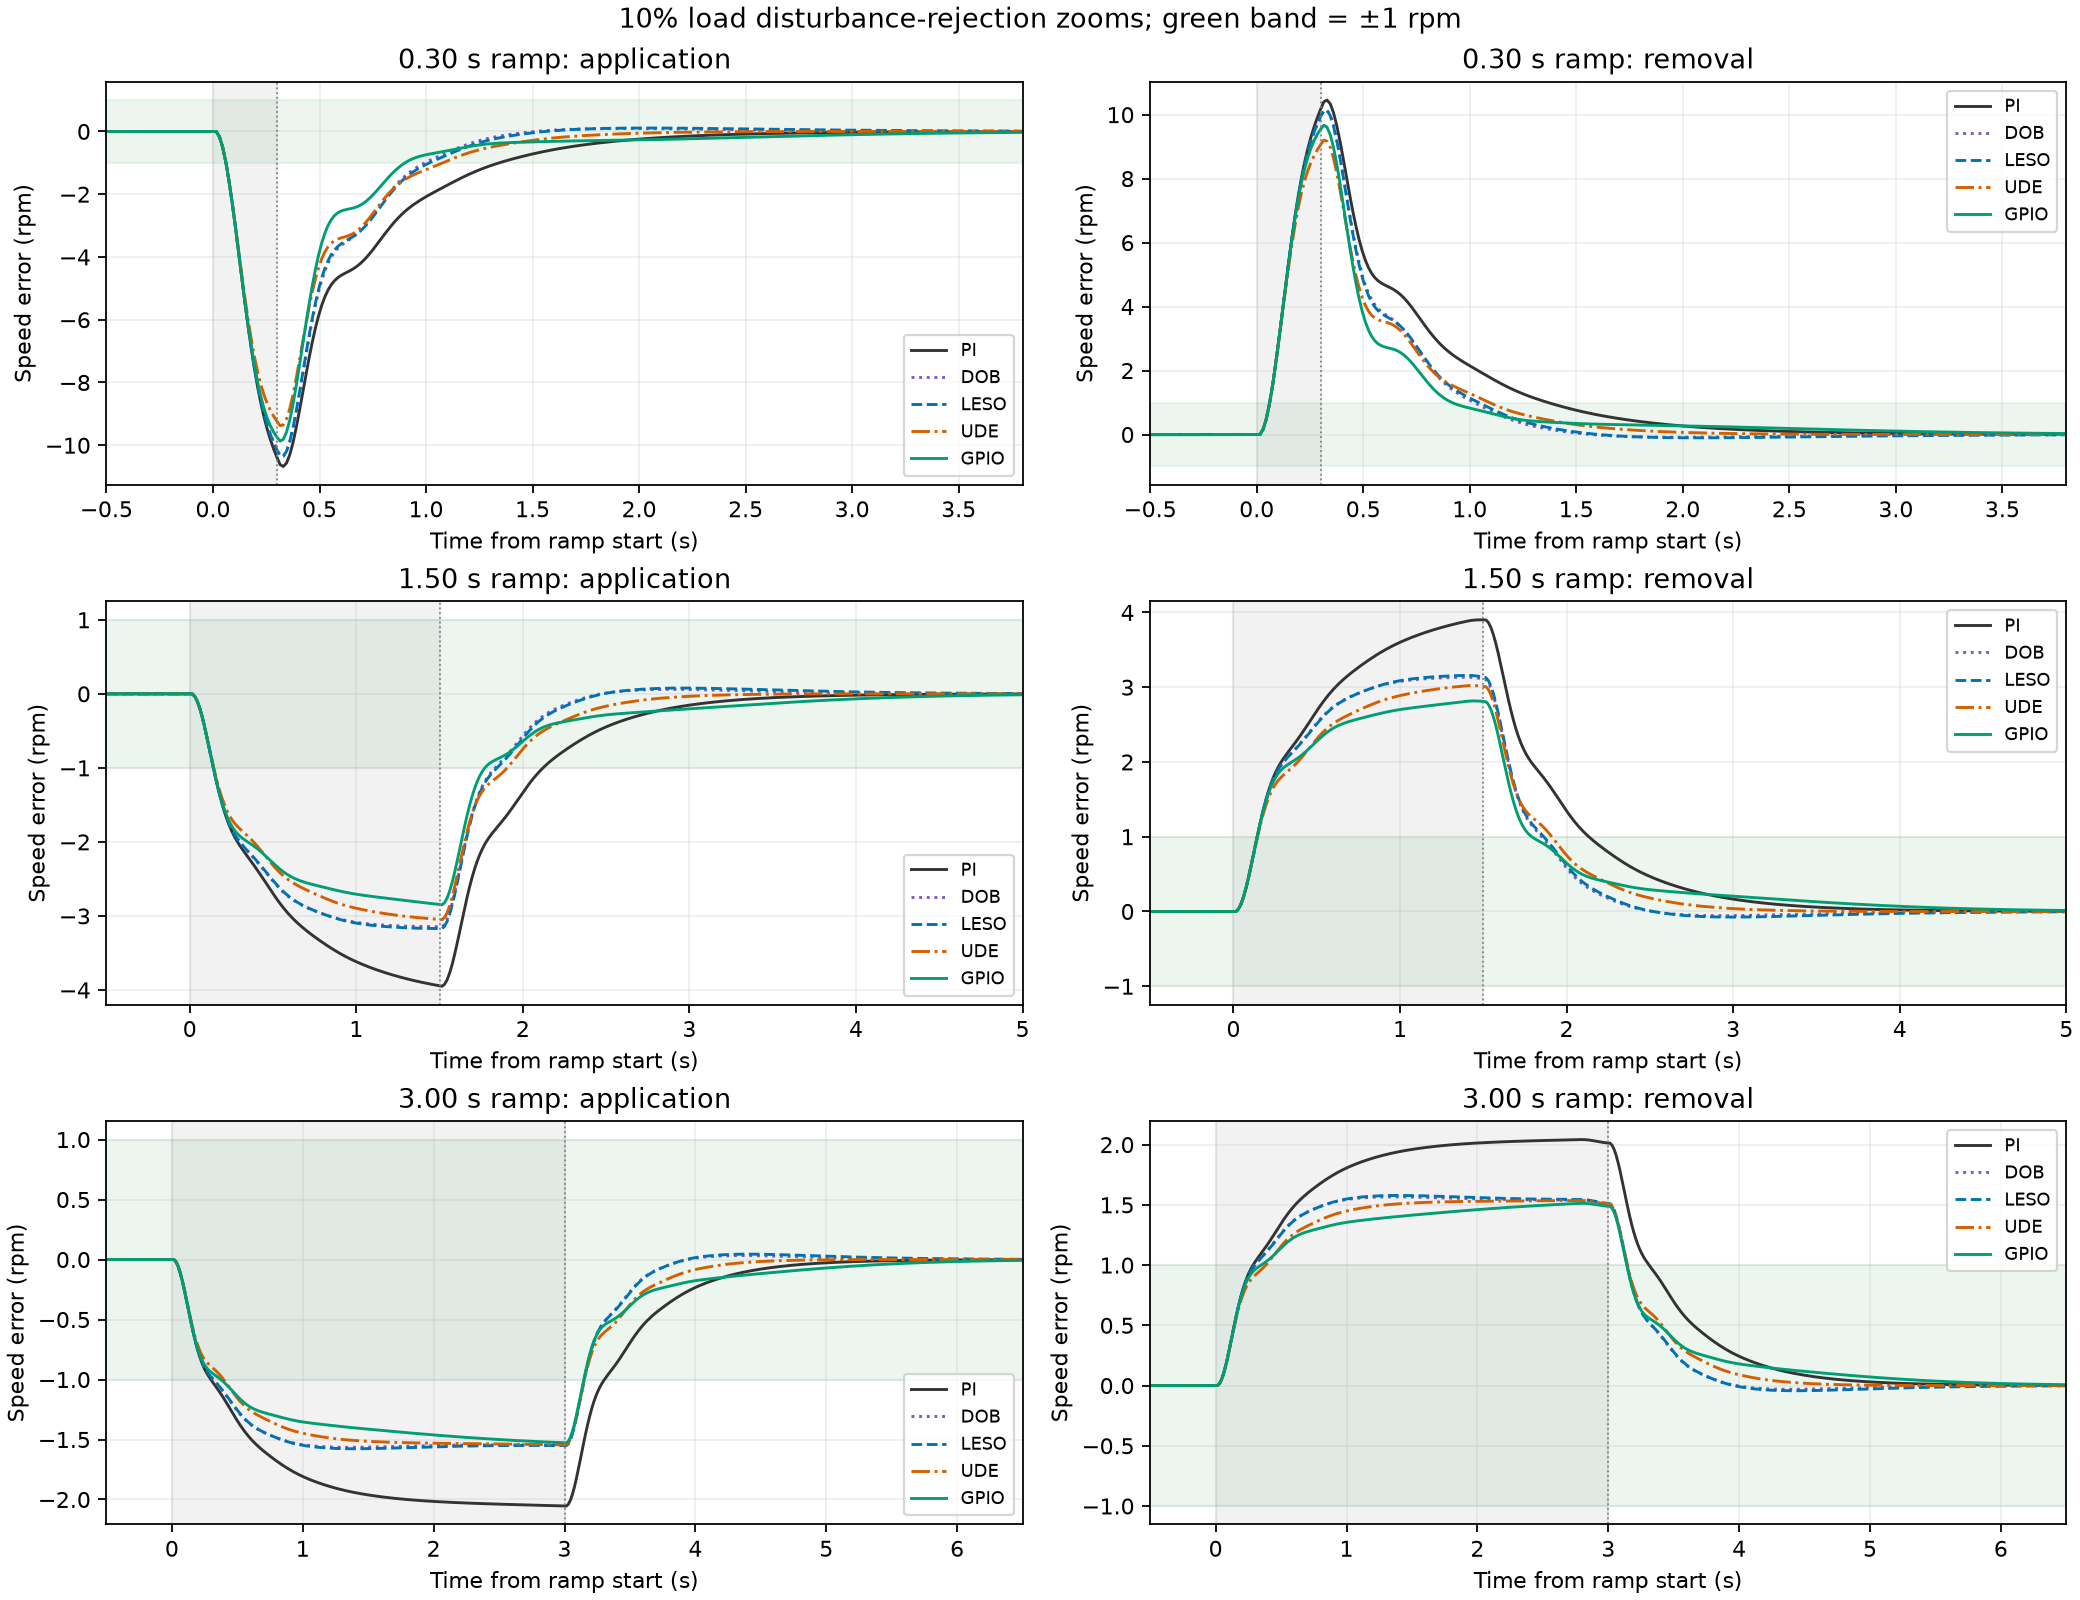
\includegraphics[width=.95\linewidth,height=.6\textheight,keepaspectratio]{early_literature_observers_9000rpm_10pct_20260912_211600_355_rejection_zooms.png}\caption{Zooms. Archived study figure.}\end{figure}

\subsection{Actuation and model validity}

{\scriptsize\setlength{\tabcolsep}{1.5mm}\begin{longtable}{>{\raggedright\arraybackslash}p{29.00mm}>{\raggedright\arraybackslash}p{29.00mm}>{\raggedright\arraybackslash}p{29.00mm}>{\raggedright\arraybackslash}p{29.00mm}>{\raggedright\arraybackslash}p{29.00mm}}\caption{LESO, UDE, and GPIO implementation and first comparison: Actuation and model validity. Archived values.}\\\toprule
Method & Fuel limit \% & Compensation clip \% & Fuel total variation lbm/s & Minimum compressor margin \%\\\midrule
\endfirsthead
Method & Fuel limit \% & Compensation clip \% & Fuel total variation lbm/s & Minimum compressor margin \%\\\midrule
\endhead
PI & 0.000 & 0.000 & 2.116 & 24.429\\
DOB & 0.000 & 0.000 & 2.136 & 24.322\\
LESO & 0.000 & 0.000 & 2.143 & 24.302\\
UDE & 0.000 & 0.000 & 2.144 & 24.389\\
GPIO & 0.000 & 0.000 & 2.174 & 24.161\\
\bottomrule\end{longtable}}

\subsection{Assessment}

\textbf{GPIO has the lowest RMSE in this fixed-setting test: 0.9509 rpm.} This is a measured result for the chosen nominal gain, observer poles and limits, not a universal ranking or optimally tuned benchmark. The existing DOB uses the fuller identified model; new observers use only its first fuel-to-acceleration coefficient as an approximate input gain.

\textbf{Practical recommendation:} start with UDE if implementation simplicity and peak rejection are the priorities; retain GPIO as the performance candidate when faster recovery justifies two extra observer states. LESO is a simpler-model substitute for the existing DOB here, but does not improve its overall RMSE. This recommendation is conditional on passing subsequent noise and robustness tests.

For the 0.30 s application ramp, post-ramp recovery is 1.050 s (PI), 0.705 s (DOB), 0.720 s (LESO), 0.780 s (UDE), and 0.615 s (GPIO). Thus UDE has the lowest peak, but is slower to enter the $\pm$1 rpm band than DOB and GPIO. For the 1.50 s ramp, GPIO application peak is 2.850 rpm versus 3.950 rpm for PI, with post-ramp recovery 0.285 versus 0.630 s. At 3.00 s, after-ramp recovery differs by only one sample or less among the augmented methods.

Relative to the existing DOB, UDE lowers RMSE by about 6.58\% and GPIO by 8.37\%. Neither fuel nor compensation saturation occurs. GPIO has the greatest fuel total variation (2.174 versus 2.116 lbm/s for PI) and the highest peak fuel (1.344 versus 1.333 lbm/s), illustrating a small actuation tradeoff. These total-variation values sum absolute sample-to-sample command changes; they are not fuel consumption.

UDE has the smallest state count and no raw derivative, but its direct speed term makes measurement-noise testing important. LESO is a simple general-purpose candidate. GPIO represents disturbance slope explicitly, at the cost of an additional state and stronger high-frequency correction. A shaft-power ramp is not necessarily a ramp in equivalent-fuel disturbance because the plant and sensor contribute to the residual.

Next compare separately tuned settings using an independent tuning case, then hold out load profiles for validation. Include sensor noise, delay variation, gain mismatch, fuel constraints and compressor margin. Do not choose a deployed method using speed RMSE alone: peak excursions, recovery, actuator variation and numerical/physical limits matter.

\subsection{Verification and reproduction}

All five actual Simulink trajectories contain 10001 samples through 150 s. Checks confirm identical shaft profiles, 9000 rpm evaluation demand, zero fuel disturbance and mechanical torque balance. The three new estimators are independently replayed from logged sensed speed and applied fuel with their exact discrete state equations. PI and existing DOB responses reproduce the preceding 10\% study. Detailed numerical errors are in verification.json.

Run \path|out=run_tmats_literature_comparison;| in MATLAB, then \path|summarize_literature_observers.py| in Python. The new model is \path|GasTurbine_Dyn_Template_GPT_DOB_PTO_ALT.mdl|; original models are preserved. Load the model first, then select an alternative with \path|tmats_literature_setup(2)| (LESO), \path|(3)| (UDE) or \path|(4)| (GPIO) before simulation; its PreLoadFcn initializes LESO by default. Observer pole stability does not establish nonlinear closed-loop robustness. No noisy or hardware experiment is claimed.


\section{Interpretation of the observer comparison} The accepted runs provide local evidence that these configured observers can reduce the recorded disturbance error. The rejected high-load cases restrict the scope of that evidence. Since load percentages are defined relative to operating-point turbine power, identical percentages at 9000 and 9500 rpm are not identical physical extraction powers. The tables compare controllers within a scenario; they do not estimate a universal observer ranking.

\chapter{Gaussian-process prediction and its control interpretation}
\label{ch:gp}
The predictor is introduced before its use in feedback. A GP posterior describes uncertainty conditional on the kernel, likelihood, and training distribution~\cite{gpml}. It is not automatically a bound on unknown external load or a certificate for feedback stability. The two-input nominal tests below therefore answer a regression question before the later chapters answer a control question.

\section{Gaussian-process regression explained from first principles}
\subsection{From a fitted curve to a distribution over functions}
Regression seeks a relationship between inputs and outputs. In the forward study the input is speed and fuel, and the output is acceleration. In the inverse study the input is speed and acceleration, and the output is fuel. A Gaussian process specifies correlated possible function values rather than choosing only a fixed polynomial form. Its mean gives a point prediction; its covariance describes uncertainty under its assumptions.

For training inputs $X=[x_1,\ldots,x_n]$ and outputs $y$, the model is $y_i=f(x_i)+\epsilon_i$, with Gaussian noise variance $\sigma_n^2$. A squared-exponential kernel is
\begin{equation}k(x,x')=\sigma_f^2\exp\left[-\frac12\sum_j\frac{(x_j-x'_j)^2}{\ell_j^2}\right].
\end{equation}
The length scales $\ell_j$ determine how rapidly similarity decays in each input direction. Different scales per input are called automatic relevance determination (ARD). They account for different smoothness and scaling, but they do not by themselves establish a causal importance ranking of physical variables.

Let $K_{ij}=k(x_i,x_j)$, $k_*=k(X,x_*)$, and $K_n=K+\sigma_n^2I$. Conditioning the joint Gaussian gives
\begin{align}\mu_*&=m(x_*)+k_*^\top K_n^{-1}(y-m(X)),\\
\sigma_{f,*}^2&=k(x_*,x_*)-k_*^\top K_n^{-1}k_*.
\end{align}
Response variance adds $\sigma_n^2$. The distinction matters when a controller schedules gains from prediction uncertainty. The project records which standard deviation is used. In computation, Cholesky factorization solves these systems; explicitly forming an inverse is unnecessary and less attractive numerically. The standard Gaussian conditioning framework is described by Rasmussen and Williams~\cite{gpml}.

\subsection{What fitting the hyperparameters does}
The negative log marginal likelihood balances data mismatch against model complexity through a quadratic term and $\log|K_n|$. A very flexible model can follow training data closely, but uncertainty and held-out errors are needed to assess generalization. The word exact in the early GP studies refers to the full Gaussian-process inference calculation on the chosen training set. It does not mean an exact physical model of the turbine or an exact representation of all available samples.

Representative input selection makes the training set cover its observed geometry. Selecting points using only inputs avoids choosing points because their test-output error looks favorable. Nevertheless, closed-loop trajectories are temporally correlated and occupy particular paths. A held-out point from a similar deterministic run is a narrower validation than an independent engine, noisy sensor, or changed ambient condition.

\subsection{Forward and inverse regression are different fits}
For $\dot N=f(N,u)$, an inverse relation $u=g(N,\dot N)$ may be useful locally. Training $g$ independently is not algebraically inverting the fitted function $f$. The mapping can also become ambiguous if unobserved thermodynamic states, external load, or environment affect acceleration. In the later four-input inverse, temperature and pressure account for some environmental dependence, but unmeasured load and internal transient states are still not explicit inputs.

At constant speed, a nominal zero-load inverse predicts nominal equilibrium fuel. An unknown external load requires extra fuel. If the controller never receives the load, evaluating the nominal inverse at the unchanged target cannot anticipate that extra demand. Feedback or a disturbance observer must infer the mismatch after it affects measured behavior.

\subsection{Prediction accuracy versus useful derivatives}
Feedback depends on how a model changes when its inputs change. A local Taylor expansion gives
\begin{equation}g(N+\delta N,a+\delta a)\simeq g(N,a)+g_N\delta N+g_a\delta a.
\end{equation}
Small average output error does not guarantee correctly signed or well-scaled $g_N$ and $g_a$. A nearly flat or negative speed derivative can turn a nominally restoring virtual-fuel signal into a weak or misleading feedback signal. This motivates the later derivative audit, separated acceleration feedback, and R3 normalization.

For example, at constant reference the dual-query error $g(r,0)-g(N_s,\hat a)$ is approximately $g_N(r-N_s)-g_a\hat a$. Proportional action on this quantity already contains a derivative-like term. Integral action on it can also alter the effective proportional behavior. Thus a controller called virtual-fuel PI can behave locally like a coupled PID. The label PI alone does not reveal the complete feedback structure.

\subsection{Uncertainty and coverage have limits}
A Gaussian posterior interval is conditional on the selected kernel, hyperparameters, noise model, training set, and included inputs. It need not include unknown load bias. A point inside each individual input's minimum and maximum can still lie outside the joint training cloud. A convex-hull check is stronger than separate range checks, but even a point inside the hull may be far from dense data. None of these geometric tests is a closed-loop stability certificate.

The forward and inverse GP studies below establish strong local prediction performance. The subsequent control chapters deliberately ask a harder question: whether acting on those predictions, their derivatives, or their uncertainty improves the actual nonlinear closed-loop response.


\section{Forward exact GP: speed and fuel to acceleration}
\textit{Evidence basis: }\path|results/exact_gpr_20260913_145742_458/REPORT.md|. The following detailed account is adapted from the archived study; references to simulation and verification describe historical work.\par

Inputs: speed N [rpm], fuel Wf [lbm/s]. Output: dN/dt [rpm/s], predictive standard deviation [rpm/s], 95\% response interval, and latent standard deviation.

Exact maximum-likelihood fit and exact prediction with ARD squared-exponential kernel. 600 training points; exactly 100 independent-experiment test points. Training uses valid chirp and selection-ramp records; validation uses a separate ramp. Training samples selected by input-only farthest-point coverage. No test outputs used for fitting or selection.

100 target speeds are linspace(9000,10000,100). Each selects the nearest unique valid recorded validation sample, without synthesizing labels. Actual speed range 9000.000000 to 9998.885249 rpm; maximum target mismatch 1.6856 rpm. Training speed 9000.0000 to 9999.8978 rpm; fuel 0,183863 to 4,194426 lbm/s.

RMSE 0.645908 rpm/s; MAE 0.510063 rpm/s; R2 0.99996430; nominal 95\% response-interval coverage 90.0\%.

Checks: power-law acceleration versus direct plant output max error 2.41e-10 rpm/s; exported Cholesky posterior versus MATLAB mean/SD errors 2.97e-09 / 2.73e-10 rpm/s.

Labels use signed compressor and turbine power and J=30: the shaft power-balance equation derived in the foundations. No finite-difference derivative is used. These records assume zero external shaft load and fixed ambient conditions. A two-input model cannot identify arbitrary changes in load, ambient conditions or hidden dynamic states. Exact refers to GP inference, not an exact physical model.

Uncertainty: latent variance = k(x,x)-||L\textbackslash{}k(X,x)||\textasciicircum{}2; response variance adds fitted noise variance. Hyperparameters are fixed at their likelihood estimate; intervals are model-conditional, not guaranteed physical error bounds or a calibrated safety bound. No test-based interval rescaling. Test points come from one trajectory and are not statistically independent replicates.

References: Volkan Aran (2019), Flexible and Robust Control of Heavy Duty Diesel Engine Airpath Using Data Driven Disturbance Observers and GPR Models, sec. 5.1, eqs. 5.5-5.14, and sec. 6.2.1. Uses per-input length scales of eq. 5.8. Thesis reference [92]: Rasmussen and Williams, Gaussian Processes for Machine Learning (2006), ch. 2, \url{https://gaussianprocess.org/gpml/chapters/RW2.pdf} . MATLAB: \url{https://www.mathworks.com/help/stats/fitrgp.html} and \url{https://www.mathworks.com/help/stats/regressiongp.predict.html} . This adapts the GP methodology to forward turbine acceleration; it does not reproduce the thesis diesel inverse controller.


\section{Inverse exact GP: desired motion to nominal fuel}
\textit{Evidence basis: }\path|results/inverse_gpr_20260913_150824_698/REPORT.md|. The following detailed account is adapted from the archived study; references to simulation and verification describe historical work.\par

Inputs: N [rpm], dN/dt [rpm/s]. Output: Wf [lbm/s], response standard deviation, 95\% response interval, and latent function standard deviation. This is a separately trained inverse regression, not an algebraic inverse of the forward GP.

Exact ARD squared-exponential GP with maximum-likelihood hyperparameters, zero mean on standardized responses, exact fitting and exact prediction. Uses the same 600 training observations and 100 held-out validation observations as the forward study. Training samples retain the original speed/fuel space-filling selection for direct comparison. Training records: valid chirp plus selection ramp; test record: separate validation ramp. No test-based tuning or interval rescaling.

Test target speeds span 9000-10000 rpm. Actual recorded speeds: 9000.000000 to 9998.885249 rpm; maximum target mismatch 1.685586 rpm. Test acceleration range: -151.003100 to 222.589628 rpm/s.

Fuel RMSE: 0.001048216 lbm/s (0.000475463 kg/s). MAE: 0.000832021 lbm/s. R2: 0.999997241. Nominal 95\% interval coverage: 97.0\% (97/100).

Exported Cholesky posterior vs MATLAB maximum mean/SD errors: 1e-11 / 4.59e-13 lbm/s. Scalar and vector API checks passed.

Training input ranges: N 9000.000000 to 9999.897804 rpm; acceleration -1153.470131 to 1076.907740 rpm/s. Training fuel range 0.183863 to 4.194426 lbm/s. The rectangular ranges do not imply every input combination is supported.

Uncertainty uses k(x,x)-||L\textbackslash{}k(X,x)||\textasciicircum{}2 for latent variance and adds fitted noise variance for response variance. All outputs are rescaled to lbm/s. Hyperparameter and input-measurement uncertainty are not integrated. Test acceleration is the plant acceleration, not a noisy numerical derivative or a forward-GP prediction.

Application: Wf\_\allowbreak hat = g(N, desired\_\allowbreak acceleration) is a candidate feedforward estimate under the original fixed ambient and zero external shaft-load conditions. Closed-loop control and varying load are not validated here. Predictions are not clipped to actuator limits. The test samples are from one trajectory; exact GP inference does not guarantee an exact or globally unique physical inverse.

Method follows Volkan Aran (2019), Flexible and Robust Control of Heavy Duty Diesel Engine Airpath Using Data Driven Disturbance Observers and GPR Models, section 5.1 equations 5.5-5.14 and inverse feedforward modeling section 6.2.1; thesis reference [92], Rasmussen and Williams, Gaussian Processes for Machine Learning, chapter 2. This adapts the methodology to T-MATS shaft dynamics.

Source forward study: \path|results/exact_gpr_20260913_145742_458|.


\section{Observer transfer and the direct GPR feedforward challenger}
\textit{Evidence basis: }\path|results/Observer_9000_9500_GPR_FF_Comparison/REPORT.md|. The following detailed account is adapted from the archived study; references to simulation and verification describe historical work.\par

GPR\_\allowbreak FF is the inverse-GP feedforward requested as GPT FF. It augments the original PI; it is not a disturbance observer. All 60 runs are new Simulink simulations. The previous five controllers at 10\% load reproduce the archived speed histories within 1e-6 rpm.

\subsection{Controller}

\begin{figure}[H]\centering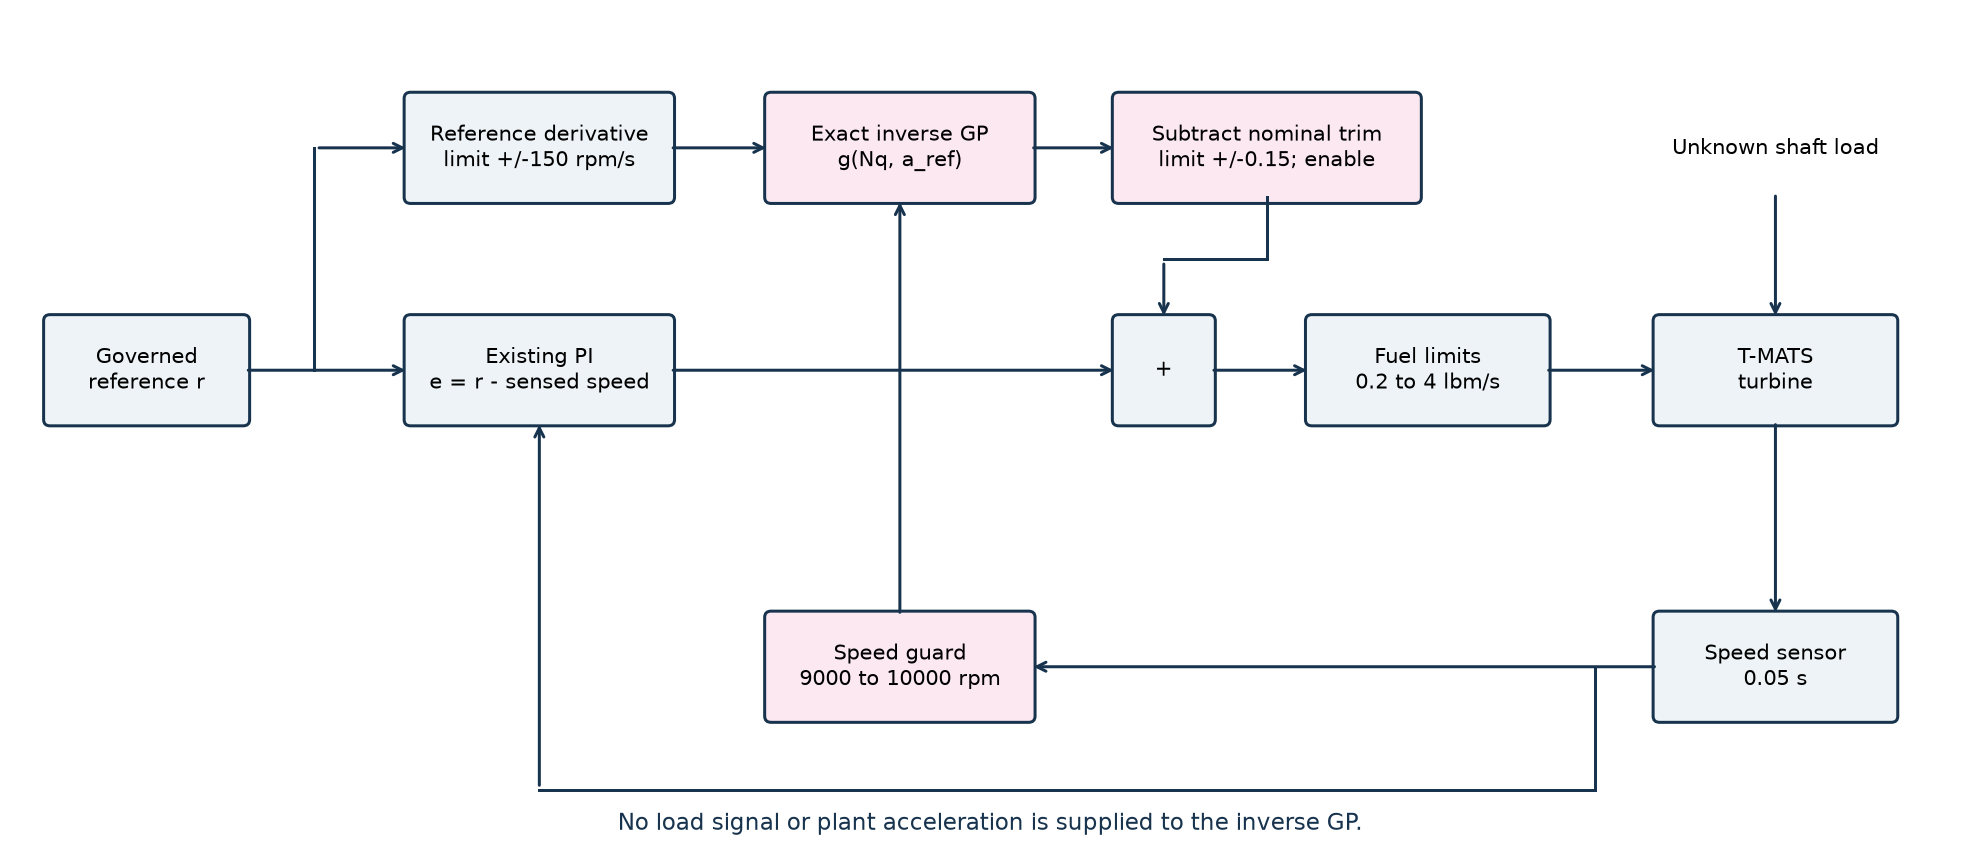
\includegraphics[width=.95\linewidth,height=.6\textheight,keepaspectratio]{early_Observer_9000_9500_GPR_FF_Comparison_controller_architecture.png}\caption{Controller architecture. Archived study figure.}\end{figure}

\texttt{a\_\allowbreak ref[k]} \texttt{=} \texttt{clip((r[k]-r[k-1])/0.015,} \texttt{-150,} \texttt{150)}

\texttt{Nq[k]} \texttt{=} \texttt{clip(N\_\allowbreak sensed[k],} \texttt{9000,} \texttt{10000)}

\par\begingroup\small\raggedright \texttt{delta\_\allowbreak u\_\allowbreak FF[k]} \texttt{=} \texttt{rho(t)} \texttt{*} \texttt{clip(g(Nq[k],a\_\allowbreak ref[k])-g(N\_\allowbreak nominal,0),} \texttt{-0.15,} \texttt{0.15)}\par\endgroup 

\texttt{u[k]} \texttt{=} \texttt{clip(u\_\allowbreak PI[k]} \texttt{+} \texttt{delta\_\allowbreak u\_\allowbreak FF[k],} \texttt{0.2,} \texttt{4)}

The original continuous PI retains Kp=0.025, Ki=0.05 and integrator initialization 3. The sensor time constant remains 0.05 s. rho ramps from 0 to 1 over absolute seconds 30-32. No observer compensation is active in GPR\_\allowbreak FF. No shaft-load value, future disturbance schedule, actual plant acceleration, or inverse-model refit is supplied to the controller.

The observer branches retain their inherited compensation gain 0.25 and pole-frequency parameter 0.5 Hz. The physical inverse-GP correction uses unit gain before the same +/-0.15 lbm/s limit; it is not bandwidth-matched to the observers. No noise, delay, or gain-tuning comparison is claimed.

This is state-scheduled nominal feedforward: sensed speed schedules the inverse model. It is not purely reference-only feedforward; that would remain constant throughout these constant-reference tests. There is no extra speed-error-to-acceleration gain. The trim subtraction prevents double-counting equilibrium fuel already supplied by the inherited PI integrator. The speed guard prevents extrapolation below the 9000 rpm training boundary, but can make the 9000 rpm response asymmetric.

The inverse model is the frozen 600-point exact ARD squared-exponential GP. Online mean evaluation is O(600); its 100-point held-out inverse fuel RMSE was 0.001048216 lbm/s and 95\% response interval coverage was 97\%. Fuel uncertainty is evaluated offline on up to 100 valid samples per control run; it is not used as a control gain or as a bound on loaded-plant error.

\subsection{Matched 10\% observer comparison}

{\scriptsize\setlength{\tabcolsep}{1.5mm}\begin{longtable}{>{\raggedright\arraybackslash}p{14.78mm}>{\raggedright\arraybackslash}p{14.78mm}>{\raggedright\arraybackslash}p{14.78mm}>{\raggedright\arraybackslash}p{14.78mm}>{\raggedright\arraybackslash}p{14.78mm}>{\raggedright\arraybackslash}p{14.78mm}>{\raggedright\arraybackslash}p{14.78mm}>{\raggedright\arraybackslash}p{14.78mm}>{\raggedright\arraybackslash}p{14.78mm}}\caption{Observer transfer and the direct GPR feedforward challenger: Matched 10\% observer comparison. Archived values.}\\\toprule
Speed & Load & Shape & Method & Valid & RMSE rpm & Peak rpm & IAE rpm s & Failure s\\\midrule
\endfirsthead
Speed & Load & Shape & Method & Valid & RMSE rpm & Peak rpm & IAE rpm s & Failure s\\\midrule
\endhead
9000 & 10\% & ramps & PI & True & 1.193 & 10.677 & 36.774 & N/A\\
9000 & 10\% & ramps & DOB & True & 1.038 & 10.351 & 28.341 & N/A\\
9000 & 10\% & ramps & LESO & True & 1.039 & 10.349 & 28.694 & N/A\\
9000 & 10\% & ramps & UDE & True & 0.969 & 9.377 & 27.587 & N/A\\
9000 & 10\% & ramps & GPIO & True & 0.951 & 9.866 & 27.577 & N/A\\
9000 & 10\% & ramps & GPR\_\allowbreak FF & True & 1.208 & 11.058 & 36.774 & N/A\\
9500 & 10\% & ramps & PI & True & 2.125 & 18.642 & 65.863 & N/A\\
9500 & 10\% & ramps & DOB & True & 1.850 & 18.147 & 50.799 & N/A\\
9500 & 10\% & ramps & LESO & True & 1.853 & 18.155 & 51.429 & N/A\\
9500 & 10\% & ramps & UDE & True & 1.730 & 16.574 & 49.411 & N/A\\
9500 & 10\% & ramps & GPIO & True & 1.698 & 17.393 & 49.392 & N/A\\
9500 & 10\% & ramps & GPR\_\allowbreak FF & True & 2.192 & 19.938 & 65.864 & N/A\\
\bottomrule\end{longtable}}

\subsection{Findings}

At 9000 rpm, GPR\_\allowbreak FF RMSE is 1.207770 rpm versus PI 1.193143 rpm (+1.23\% change; positive is worse). Peak error is 11.057788 rpm. Speed guard active: 34.04\% of evaluation samples.
GPR\_\allowbreak FF +/-1 rpm recovery at 9000 rpm is faster than PI in 3/6 events, equal in 3/6, and slower in 0/6. Thus the larger peaks and RMSE coexist with faster threshold recovery; these metrics must not be collapsed into a single blanket ranking.
At 9500 rpm, GPR\_\allowbreak FF RMSE is 2.191826 rpm versus PI 2.125136 rpm (+3.14\% change; positive is worse). Peak error is 19.937677 rpm. Speed guard active: 0.00\% of evaluation samples.
GPR\_\allowbreak FF +/-1 rpm recovery at 9500 rpm is faster than PI in 6/6 events, equal in 0/6, and slower in 0/6. Thus the larger peaks and RMSE coexist with faster threshold recovery; these metrics must not be collapsed into a single blanket ranking.

A nominal inverse learned at zero external shaft load cannot anticipate an unknown load. Accurate offline inverse regression does not imply improved rejection. In these tests a\_\allowbreak ref is zero during evaluation, so the FF branch only schedules nominal fuel with sensed speed; the PI integrator supplies the additional load-dependent fuel. A learned increase in equilibrium fuel with speed can reduce effective restoring feedback when added to the unchanged PI. Results are reported without retuning to favor the GP.

Regression of unclipped FF correction against sensed speed on the matched runs gives slopes 0.0015974 and 0.0020183 lbm/s per rpm at 9000 and 9500 rpm, respectively. These are descriptive trajectory fits, not independent linearizations; the 9000 rpm fit excludes the active speed guard.

\subsection{All load scenarios}

{\scriptsize\setlength{\tabcolsep}{1.5mm}\begin{longtable}{>{\raggedright\arraybackslash}p{14.78mm}>{\raggedright\arraybackslash}p{14.78mm}>{\raggedright\arraybackslash}p{14.78mm}>{\raggedright\arraybackslash}p{14.78mm}>{\raggedright\arraybackslash}p{14.78mm}>{\raggedright\arraybackslash}p{14.78mm}>{\raggedright\arraybackslash}p{14.78mm}>{\raggedright\arraybackslash}p{14.78mm}>{\raggedright\arraybackslash}p{14.78mm}}\caption{Observer transfer and the direct GPR feedforward challenger: All load scenarios. Archived values.}\\\toprule
Speed & Load & Shape & Method & Valid & RMSE rpm & Peak rpm & IAE rpm s & Failure s\\\midrule
\endfirsthead
Speed & Load & Shape & Method & Valid & RMSE rpm & Peak rpm & IAE rpm s & Failure s\\\midrule
\endhead
9000 & 5\% & ramps & PI & True & 0.594 & 5.325 & 18.309 & N/A\\
9000 & 5\% & ramps & DOB & True & 0.517 & 5.162 & 14.109 & N/A\\
9000 & 5\% & ramps & LESO & True & 0.517 & 5.161 & 14.285 & N/A\\
9000 & 5\% & ramps & UDE & True & 0.483 & 4.677 & 13.735 & N/A\\
9000 & 5\% & ramps & GPIO & True & 0.473 & 4.920 & 13.730 & N/A\\
9000 & 5\% & ramps & GPR\_\allowbreak FF & True & 0.601 & 5.515 & 18.309 & N/A\\
9000 & 10\% & ramps & PI & True & 1.193 & 10.677 & 36.774 & N/A\\
9000 & 10\% & ramps & DOB & True & 1.038 & 10.351 & 28.341 & N/A\\
9000 & 10\% & ramps & LESO & True & 1.039 & 10.349 & 28.694 & N/A\\
9000 & 10\% & ramps & UDE & True & 0.969 & 9.377 & 27.587 & N/A\\
9000 & 10\% & ramps & GPIO & True & 0.951 & 9.866 & 27.577 & N/A\\
9000 & 10\% & ramps & GPR\_\allowbreak FF & True & 1.208 & 11.058 & 36.774 & N/A\\
9000 & 20\% & ramps & PI & True & 2.540 & 22.553 & 78.110 & N/A\\
9000 & 20\% & ramps & DOB & True & 2.237 & 22.329 & 60.838 & N/A\\
9000 & 20\% & ramps & LESO & True & 2.240 & 22.335 & 61.314 & N/A\\
9000 & 20\% & ramps & UDE & False & N/A & N/A & N/A & 61.530\\
9000 & 20\% & ramps & GPIO & True & 2.072 & 21.457 & 60.111 & N/A\\
9000 & 20\% & ramps & GPR\_\allowbreak FF & True & 2.571 & 23.707 & 78.110 & N/A\\
9000 & 30\% & ramps & PI & True & 3.973 & 35.359 & 121.624 & N/A\\
9000 & 30\% & ramps & DOB & True & 3.664 & 35.258 & 104.370 & N/A\\
9000 & 30\% & ramps & LESO & True & 3.668 & 35.258 & 105.042 & N/A\\
9000 & 30\% & ramps & UDE & True & 3.530 & 35.237 & 103.631 & N/A\\
9000 & 30\% & ramps & GPIO & True & 3.501 & 35.258 & 103.625 & N/A\\
9000 & 30\% & ramps & GPR\_\allowbreak FF & True & 4.022 & 37.310 & 121.624 & N/A\\
9500 & 5\% & ramps & PI & True & 1.017 & 8.905 & 31.538 & N/A\\
9500 & 5\% & ramps & DOB & True & 0.885 & 8.667 & 24.317 & N/A\\
9500 & 5\% & ramps & LESO & True & 0.886 & 8.670 & 24.619 & N/A\\
9500 & 5\% & ramps & UDE & True & 0.827 & 7.905 & 23.660 & N/A\\
9500 & 5\% & ramps & GPIO & True & 0.811 & 8.281 & 23.651 & N/A\\
9500 & 5\% & ramps & GPR\_\allowbreak FF & True & 1.049 & 9.513 & 31.538 & N/A\\
9500 & 10\% & ramps & PI & True & 2.125 & 18.642 & 65.863 & N/A\\
9500 & 10\% & ramps & DOB & True & 1.850 & 18.147 & 50.799 & N/A\\
9500 & 10\% & ramps & LESO & True & 1.853 & 18.155 & 51.429 & N/A\\
9500 & 10\% & ramps & UDE & True & 1.730 & 16.574 & 49.411 & N/A\\
9500 & 10\% & ramps & GPIO & True & 1.698 & 17.393 & 49.392 & N/A\\
9500 & 10\% & ramps & GPR\_\allowbreak FF & True & 2.192 & 19.938 & 65.864 & N/A\\
9500 & 20\% & ramps & PI & True & 4.453 & 39.270 & 137.688 & N/A\\
9500 & 20\% & ramps & DOB & True & 4.148 & 39.270 & 120.437 & N/A\\
9500 & 20\% & ramps & LESO & True & 4.152 & 39.270 & 121.213 & N/A\\
9500 & 20\% & ramps & UDE & True & 4.024 & 39.270 & 119.694 & N/A\\
9500 & 20\% & ramps & GPIO & True & 3.985 & 39.270 & 119.688 & N/A\\
9500 & 20\% & ramps & GPR\_\allowbreak FF & True & 4.593 & 41.941 & 137.689 & N/A\\
9500 & 30\% & ramps & PI & False & N/A & N/A & N/A & 10.380\\
9500 & 30\% & ramps & DOB & False & N/A & N/A & N/A & 10.380\\
9500 & 30\% & ramps & LESO & False & N/A & N/A & N/A & 10.380\\
9500 & 30\% & ramps & UDE & False & N/A & N/A & N/A & 10.380\\
9500 & 30\% & ramps & GPIO & False & N/A & N/A & N/A & 10.365\\
9500 & 30\% & ramps & GPR\_\allowbreak FF & False & N/A & N/A & N/A & 10.380\\
9500 & 20\% & steps & PI & True & 6.430 & 54.100 & 137.688 & N/A\\
9500 & 20\% & steps & DOB & True & 6.203 & 54.100 & 120.508 & N/A\\
9500 & 20\% & steps & LESO & True & 6.207 & 54.100 & 121.530 & N/A\\
9500 & 20\% & steps & UDE & True & 5.989 & 54.100 & 119.694 & N/A\\
9500 & 20\% & steps & GPIO & True & 6.016 & 54.100 & 119.688 & N/A\\
9500 & 20\% & steps & GPR\_\allowbreak FF & True & 6.712 & 56.329 & 137.689 & N/A\\
9500 & 30\% & steps & PI & False & N/A & N/A & N/A & 10.155\\
9500 & 30\% & steps & DOB & False & N/A & N/A & N/A & 10.155\\
9500 & 30\% & steps & LESO & False & N/A & N/A & N/A & 10.155\\
9500 & 30\% & steps & UDE & False & N/A & N/A & N/A & 10.140\\
9500 & 30\% & steps & GPIO & False & N/A & N/A & N/A & 10.155\\
9500 & 30\% & steps & GPR\_\allowbreak FF & False & N/A & N/A & N/A & 10.155\\
\bottomrule\end{longtable}}

At both speeds, 5\%, 10\%, 20\%, and 30\% gross-turbine-power extraction uses three ramp/hold/ramp pulses (0.30, 1.50, 3.00 s). The earlier 9500 rpm 20\% and 30\% step-load cases are repeated too. Application times are 10.005, 30, 60 s; removal times 15, 40.005, 75 s after 60 s preparation. The 9500 rpm ramped 5/20/30\% cases extend the previous matrix. Loads are speed-specific fractions, not equal absolute powers.

\subsection{Validity and recovery}

Validity requires finite logged signals, positive fuel, positive compressor margin, flow residual <=1e-9, and fewer than 200 iterations. Full-run scores are withheld after any invalid solve; plots show only the valid prefix. A later numerically converged sample does not rehabilitate the trajectory. Shaft balance and command reconstruction are verified independently. Identical load profiles are checked across methods.

Recovery is the first sample after the last excursion outside +/-1 rpm with at least 0.5 s dwell before the next load edge. After-ramp recovery subtracts ramp duration and is bounded below by zero. Event scores are withheld if any preceding sample is invalid. All 360 event records are in events.csv.

\subsection{Reproduce}

\path|run_tmats_gpr_ff_benchmarks| builds GasTurbine\_\allowbreak Dyn\_\allowbreak Template\_\allowbreak GPR\_\allowbreak FF.mdl and runs the matrix. Then run \path|summarize_tmats_gpr_ff.py|. The previous models and trained inverse GP remain separate. The new Level-2 MATLAB S-function is a desktop simulation implementation, not an embedded code-generation claim.

References: Aran (2019), thesis sections 5.1 and 6.2.1; Rasmussen and Williams, Gaussian Processes for Machine Learning, chapter 2. Previous report derivations for the inherited PI/DOB/LESO/UDE/GPIO remain applicable.

\subsection{9000 rpm plots}

\begin{figure}[H]\centering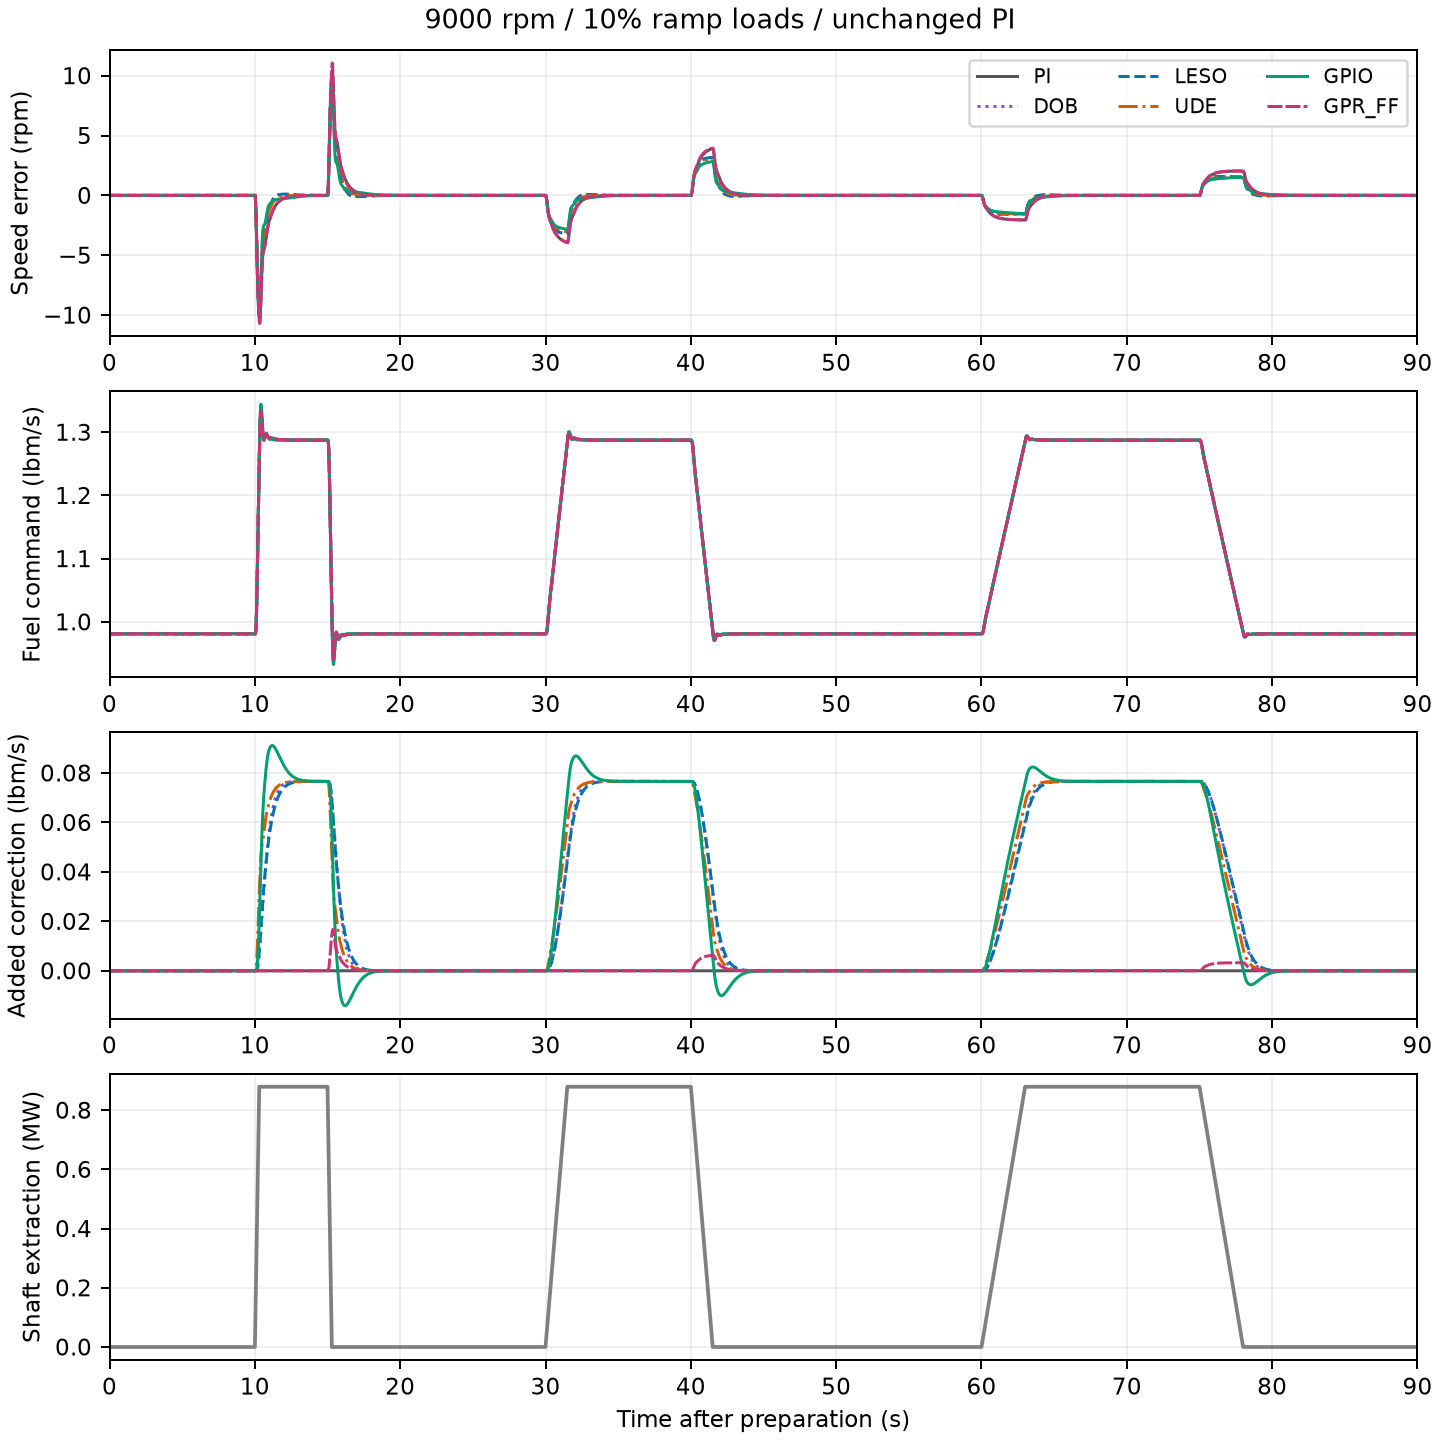
\includegraphics[width=.95\linewidth,height=.6\textheight,keepaspectratio]{early_Observer_9000_9500_GPR_FF_Comparison_overview_9000.png}\caption{Six-controller response. Archived study figure.}\end{figure}

\begin{figure}[H]\centering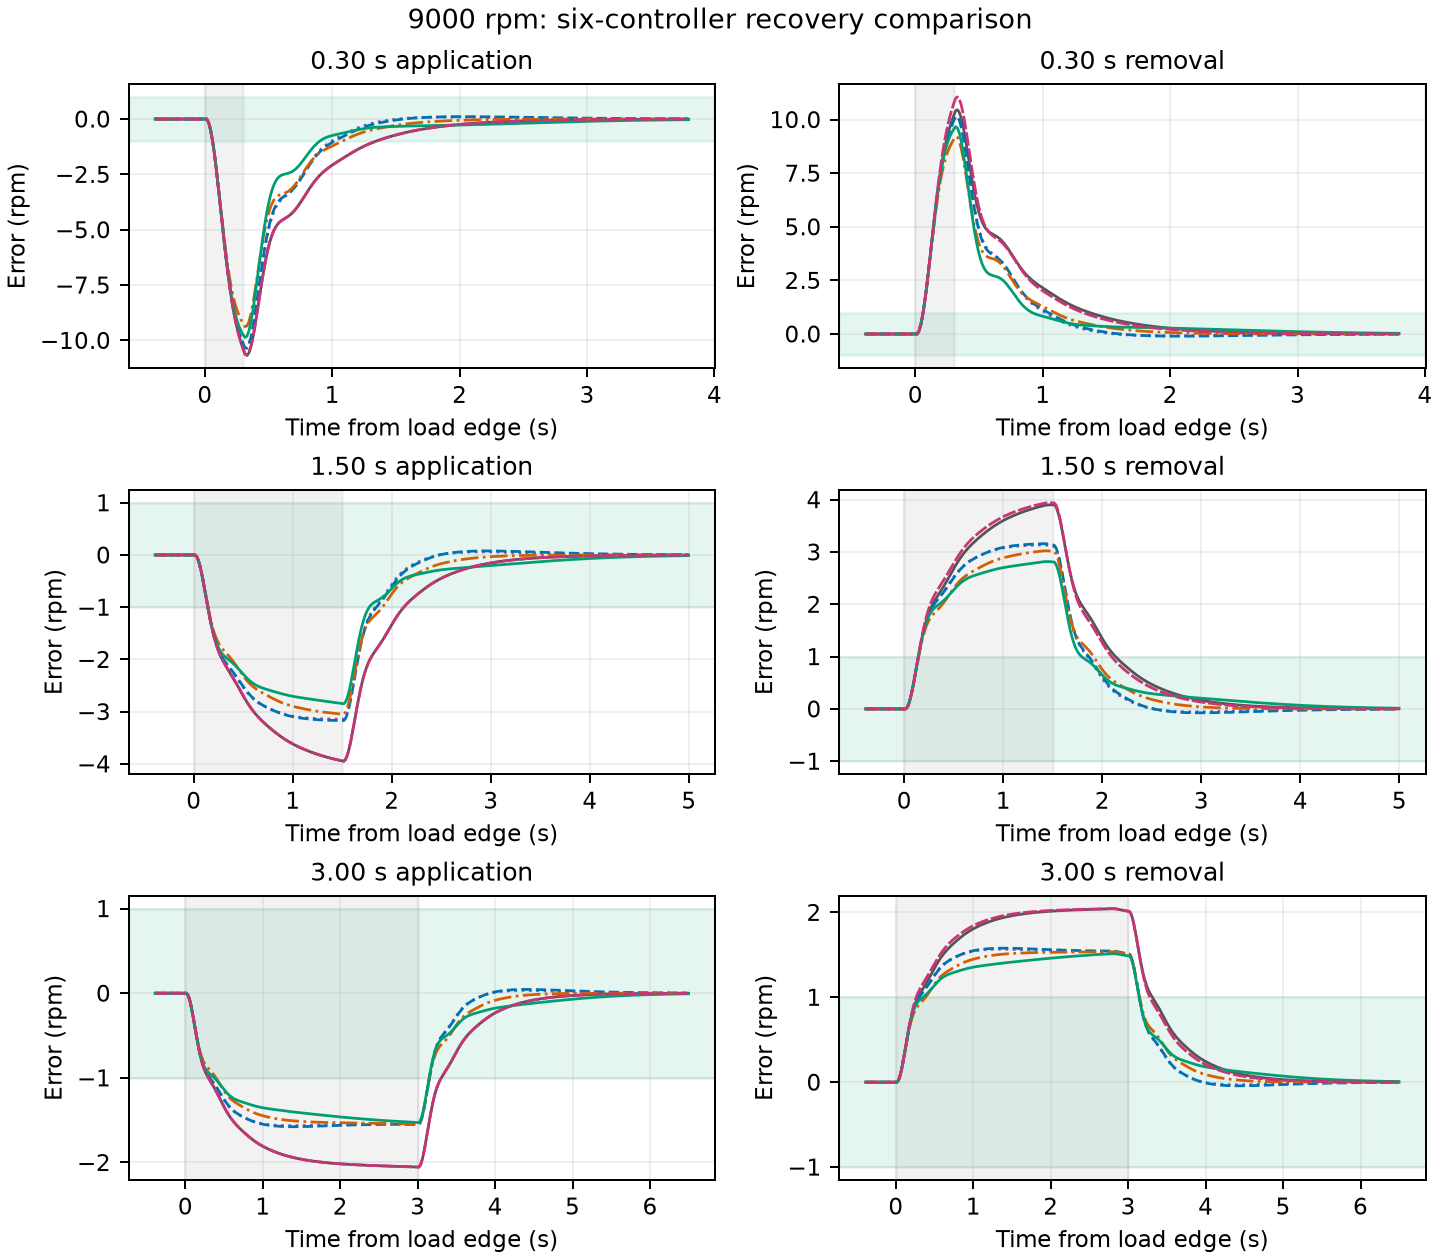
\includegraphics[width=.95\linewidth,height=.6\textheight,keepaspectratio]{early_Observer_9000_9500_GPR_FF_Comparison_zooms_9000.png}\caption{Recovery zooms. Archived study figure.}\end{figure}

\subsection{9500 rpm plots}

\begin{figure}[H]\centering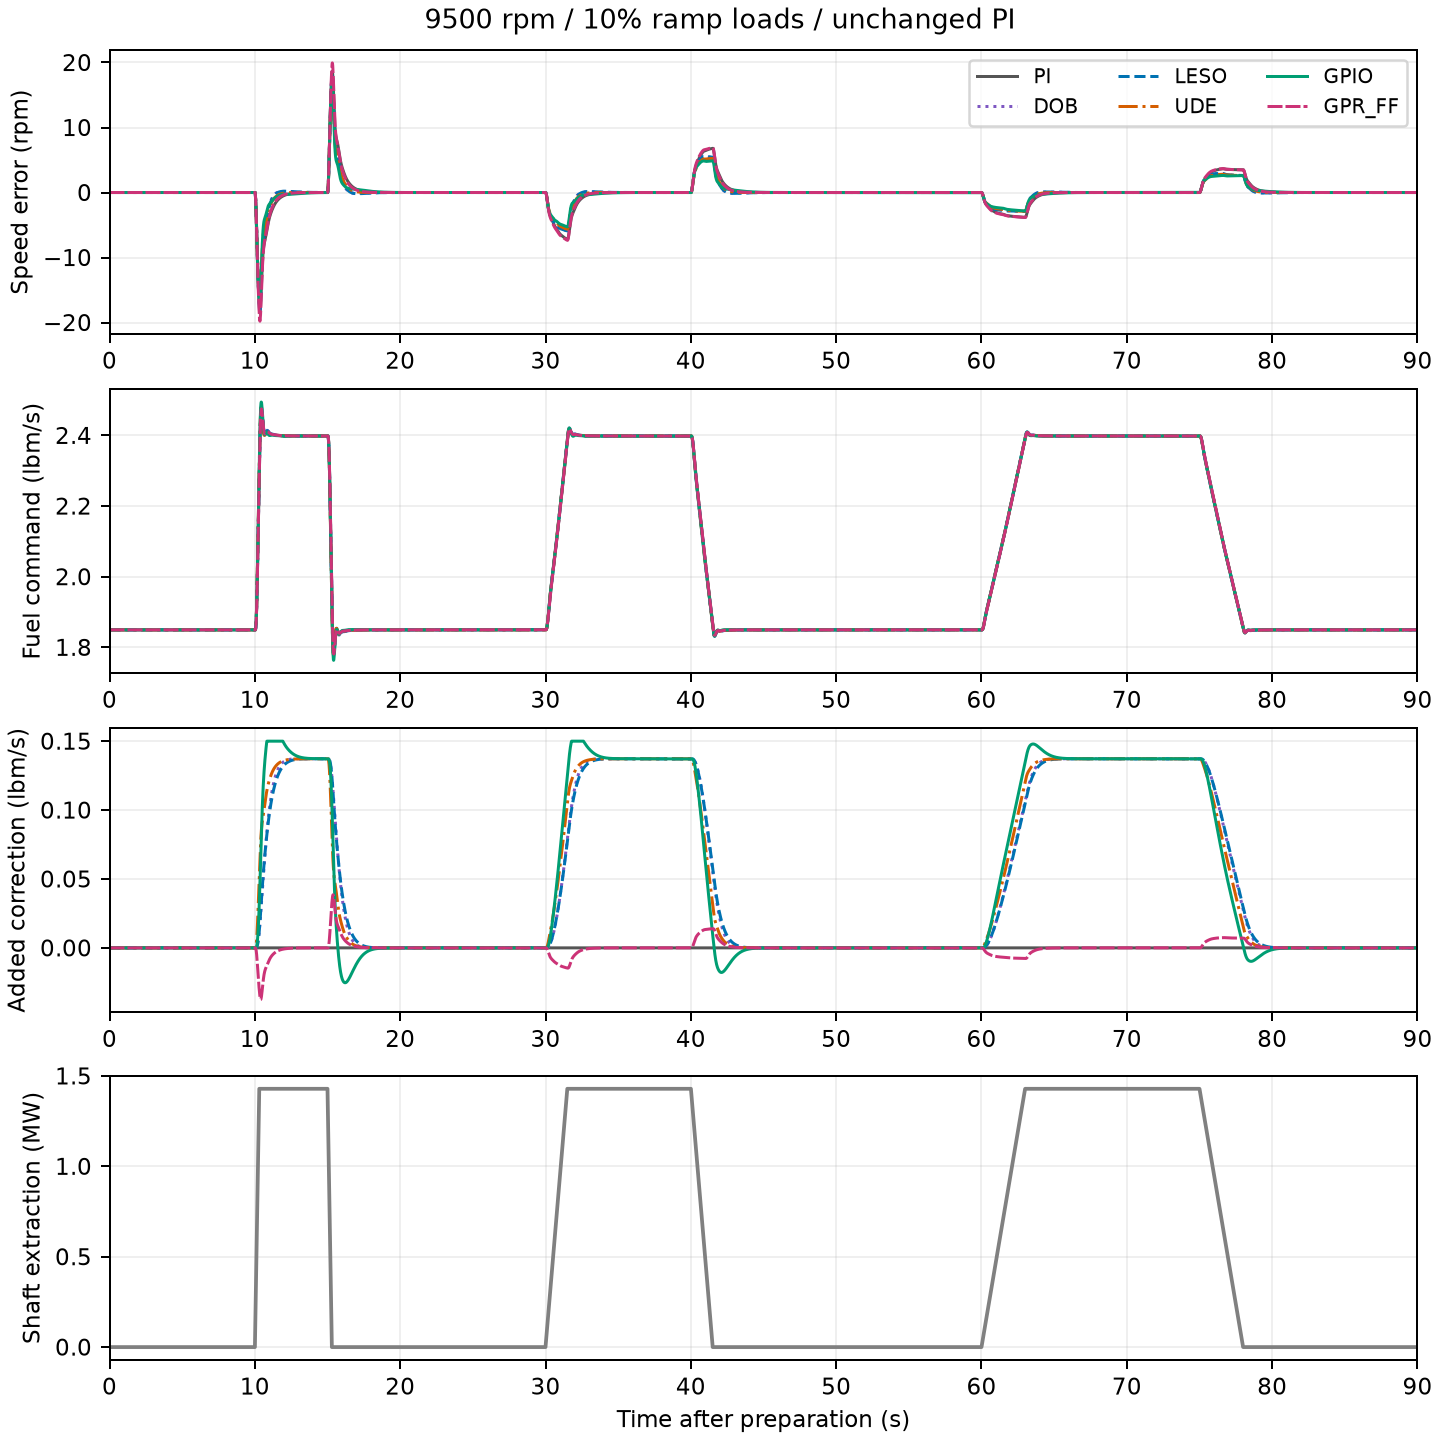
\includegraphics[width=.95\linewidth,height=.6\textheight,keepaspectratio]{early_Observer_9000_9500_GPR_FF_Comparison_overview_9500.png}\caption{Six-controller response. Archived study figure.}\end{figure}

\begin{figure}[H]\centering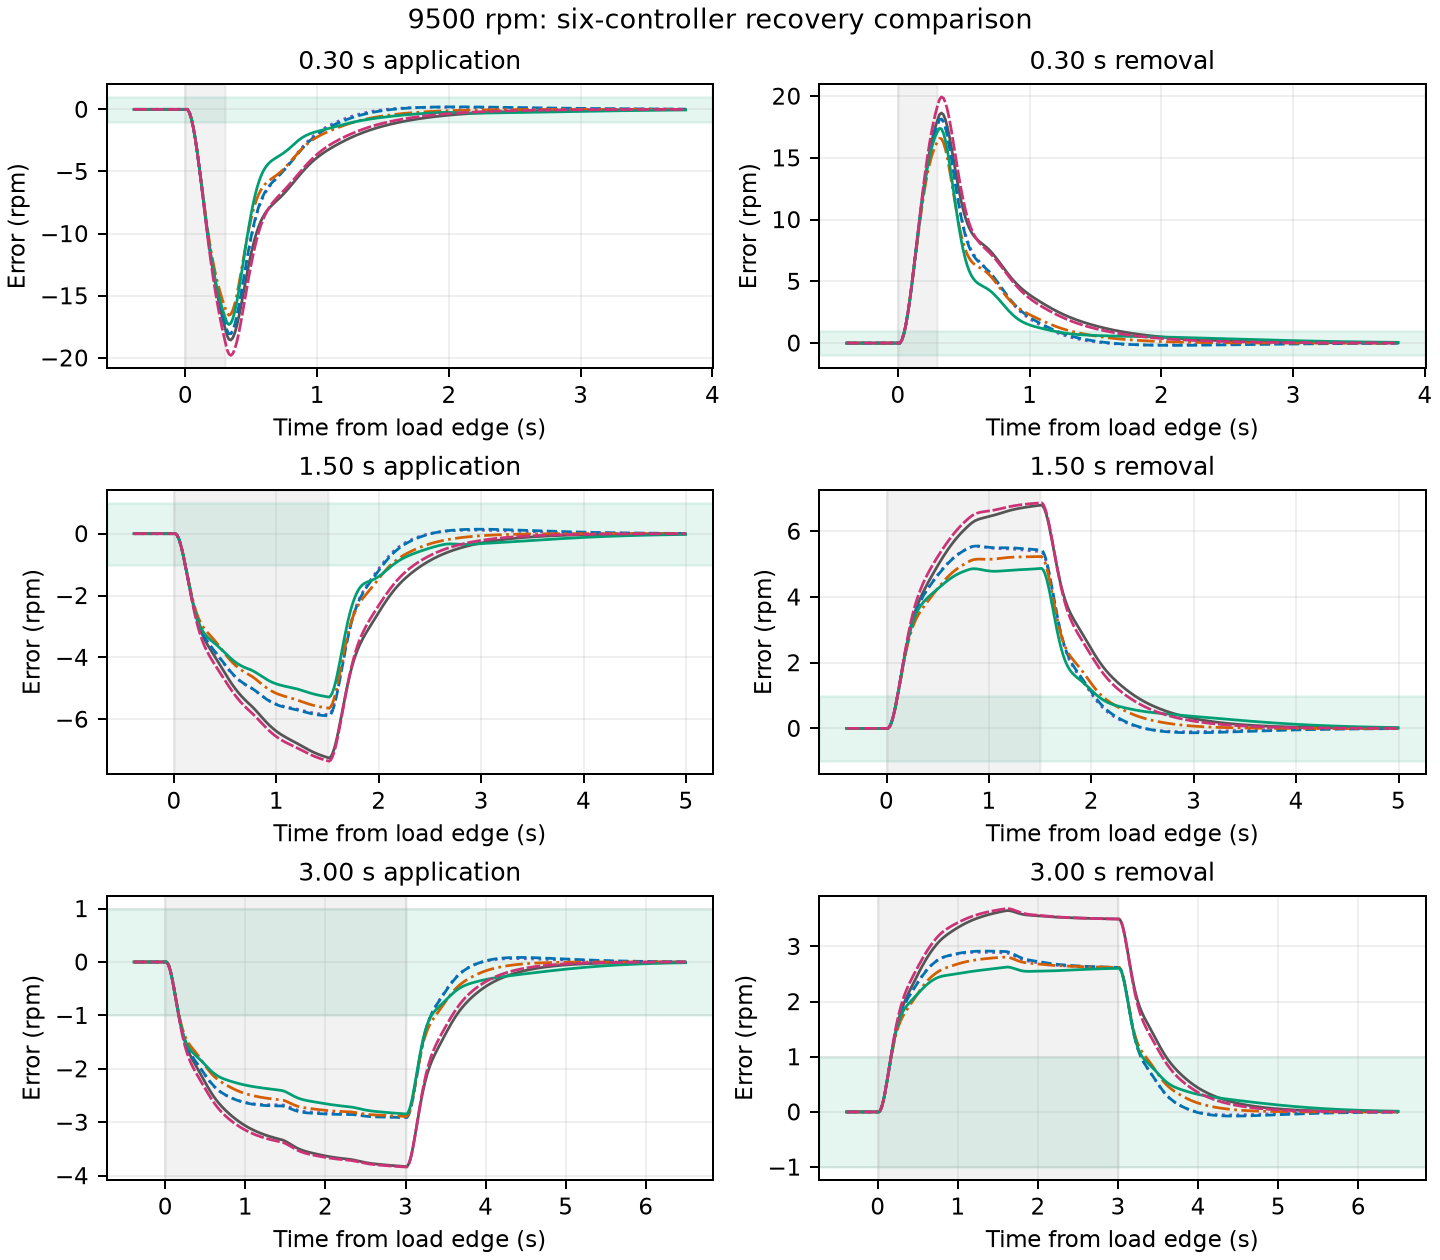
\includegraphics[width=.95\linewidth,height=.6\textheight,keepaspectratio]{early_Observer_9000_9500_GPR_FF_Comparison_zooms_9500.png}\caption{Recovery zooms. Archived study figure.}\end{figure}

\subsection{First-invalid-sample diagnostics}

{\scriptsize\setlength{\tabcolsep}{1.5mm}\begin{longtable}{>{\raggedright\arraybackslash}p{23.67mm}>{\raggedright\arraybackslash}p{23.67mm}>{\raggedright\arraybackslash}p{23.67mm}>{\raggedright\arraybackslash}p{23.67mm}>{\raggedright\arraybackslash}p{23.67mm}>{\raggedright\arraybackslash}p{23.67mm}}\caption{Observer transfer and the direct GPR feedforward challenger: First-invalid-sample diagnostics. Archived values.}\\\toprule
Scenario & Method & Time s & Flow residual & Iterations & Margin \%\\\midrule
\endfirsthead
Scenario & Method & Time s & Flow residual & Iterations & Margin \%\\\midrule
\endhead
9000rpm\_\allowbreak 20pct\_\allowbreak ramps & UDE & 61.530 & 1.45e-05 & 200 & 25.679\\
9500rpm\_\allowbreak 30pct\_\allowbreak ramps & PI & 10.380 & 0.00119 & 200 & 0.000\\
9500rpm\_\allowbreak 30pct\_\allowbreak ramps & DOB & 10.380 & 0.00304 & 200 & 0.000\\
9500rpm\_\allowbreak 30pct\_\allowbreak ramps & LESO & 10.380 & 0.00332 & 200 & 0.000\\
9500rpm\_\allowbreak 30pct\_\allowbreak ramps & UDE & 10.380 & 0.000294 & 200 & 0.000\\
9500rpm\_\allowbreak 30pct\_\allowbreak ramps & GPIO & 10.365 & 8.86e-05 & 200 & 0.000\\
9500rpm\_\allowbreak 30pct\_\allowbreak ramps & GPR\_\allowbreak FF & 10.380 & 0.000656 & 200 & 0.000\\
9500rpm\_\allowbreak 30pct\_\allowbreak steps & PI & 10.155 & 0.00647 & 200 & 0.000\\
9500rpm\_\allowbreak 30pct\_\allowbreak steps & DOB & 10.155 & 0.00804 & 200 & 0.000\\
9500rpm\_\allowbreak 30pct\_\allowbreak steps & LESO & 10.155 & 0.00801 & 200 & 0.000\\
9500rpm\_\allowbreak 30pct\_\allowbreak steps & UDE & 10.140 & 0.00154 & 200 & 0.000\\
9500rpm\_\allowbreak 30pct\_\allowbreak steps & GPIO & 10.155 & 0.0107 & 200 & 0.000\\
9500rpm\_\allowbreak 30pct\_\allowbreak steps & GPR\_\allowbreak FF & 10.155 & 0.00119 & 200 & 0.000\\
\bottomrule\end{longtable}}
\subsection{Wider load tests}

\begin{figure}[H]\centering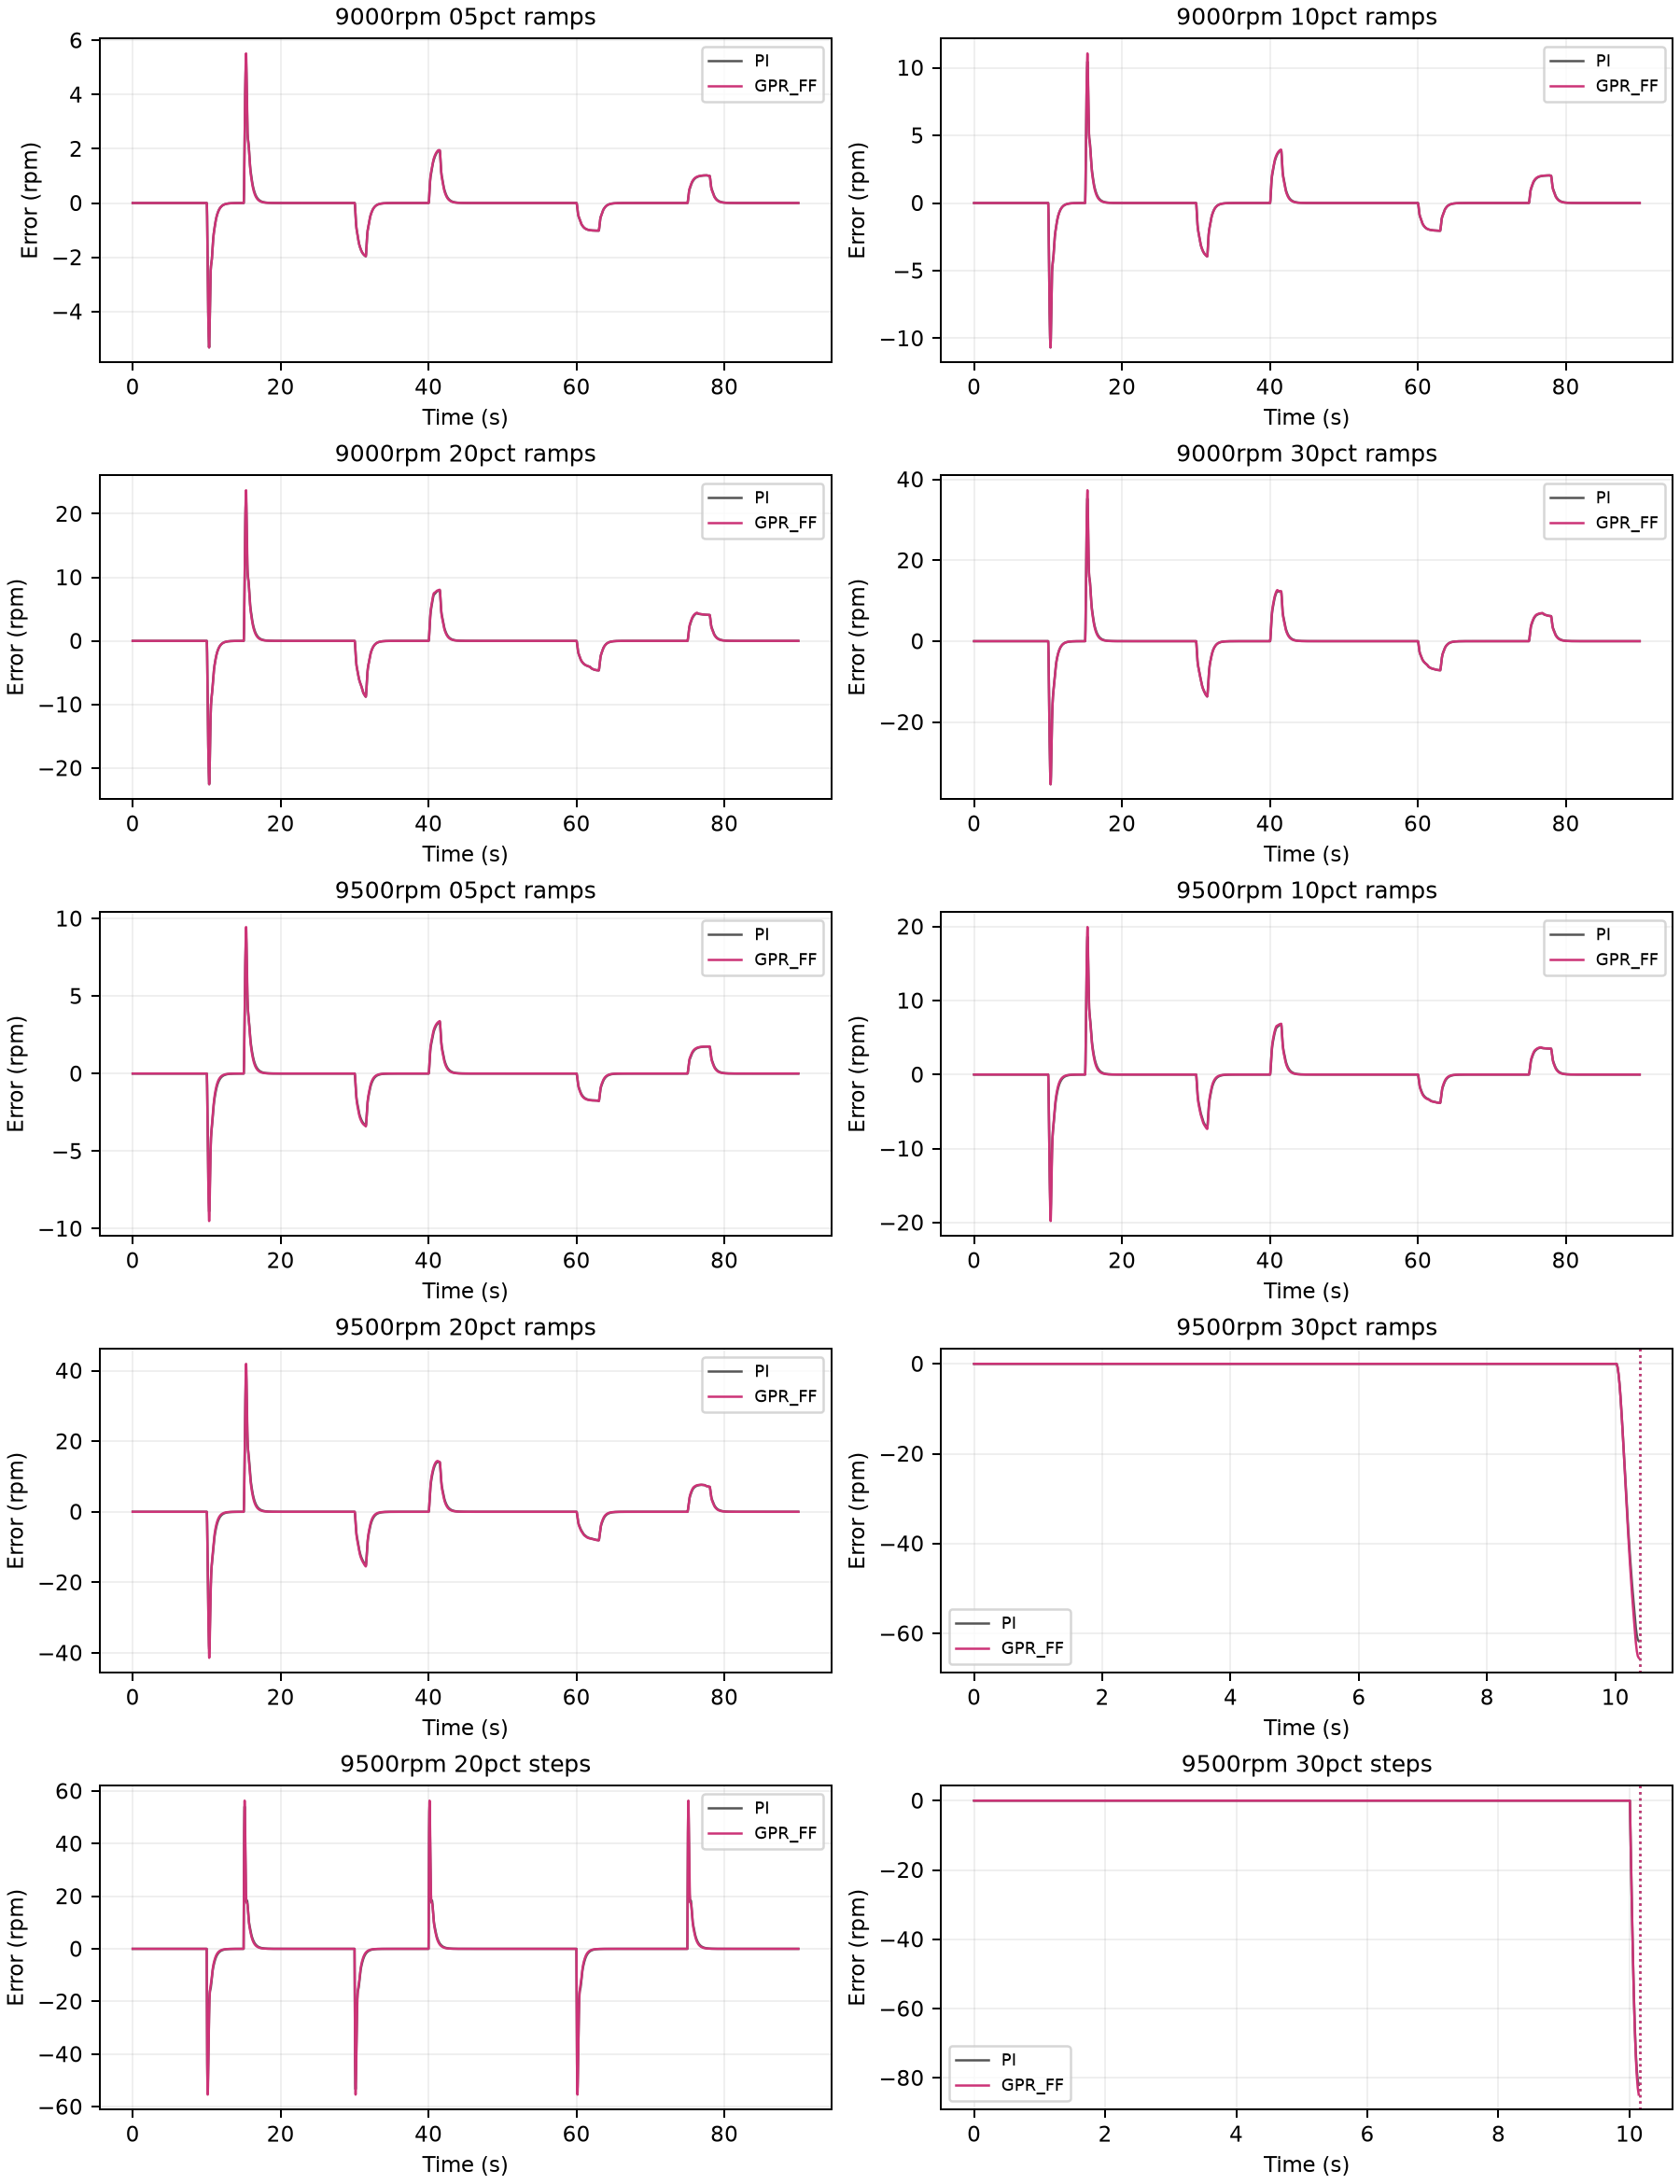
\includegraphics[width=.95\linewidth,height=.6\textheight,keepaspectratio]{early_Observer_9000_9500_GPR_FF_Comparison_all_loads.png}\caption{All loads. Archived study figure.}\end{figure}



\chapter{Inverse-coordinate feedback, feedforward, and gain selection}
\label{ch:inverse}
The central attribution question is whether improvement belongs to the inverse model, the feedback coordinates, or gain selection. This chapter retains the exact algorithm distinctions and the fixed-reference feedforward equivalence. Its conclusions concern the September controller family; the later PILCO-style chapter uses a separate dynamics GP.

\section{Protocol for the inverse-model controller comparisons}
\subsection{Simulation plant and physical interpretation}
T-MATS supplies modular thermodynamic components and iterative solution machinery for steady and dynamic propulsion-system models~\cite{tmats,tmatscode}. The local study uses its inherited nonlinear gas-turbine configuration. The controller actuates fuel flow and observes a filtered shaft-speed signal. External shaft power is applied to the plant, not supplied to the inverse model or controller as a measured feedforward signal.

A physical bookkeeping equation in consistent SI units is
\begin{equation}
J\dot\omega=\tau_t-\tau_c-\tau_L,\qquad \omega=\frac{2\pi N}{60},\qquad \tau_L=\frac{P_L}{\omega}.
\label{eq:shaft}
\end{equation}
Equation~\eqref{eq:shaft} expresses the shaft-power mechanism; it is not a replacement for the archived nonlinear T-MATS component model. The simulation interface expresses load power in hp and fuel in lbm/s. Multiplication by 0.45359237 converts fuel flow to kg/s. A load fraction is a fraction of the condition-specific unloaded turbine shaft-power reference, not a fraction of fuel flow or a prescribed speed decrease.

\subsection{Notation and controller timing}
\begin{longtable}{@{}p{.16\linewidth}p{.54\linewidth}p{.23\linewidth}@{}}
\toprule Symbol & Meaning & Unit\\\midrule
$N,N_s,r$ & Actual speed, sensed speed, governed request & rpm\\
$\hat a,a_r$ & Filtered sensed acceleration, explicit reference acceleration & rpm/s\\
$T,P$ & Sample-delayed inlet values used by the online inverse & K, kPa\\
$u,u^\star,I$ & Limited fuel, unsaturated fuel, integral contribution & lbm/s\\
$g,p_2$ & GP and full quadratic inverse means & lbm/s\\
$e_v,e_0$ & Dynamic virtual-fuel error, static inverse error & lbm/s\\
$e_N^g,a^g$ & Derivative-normalized speed error and acceleration & rpm, rpm/s\\
$g_N,g_a$ & Partial derivatives of the inverse mean & fuel/rpm, fuel/(rpm/s)\\
$T_s,\tau_s,\tau_a$ & Sample interval, speed-sensor and acceleration-filter constants & s\\
$R_L,R_C$ & Load-edge ringing and cycle-segment fuel reversal & lbm/s\\
\bottomrule
\end{longtable}
The controller interval is $T_s=0.015$ s. The inherited speed sensor has time constant $\tau_s=0.05$ s, and the inverse controllers use $\tau_a=0.03$ s for acceleration estimation. The reported tests have no newly introduced sensor noise or actuator lag. Actual plant acceleration is recorded for identification and validation; the online feedback acceleration is reconstructed from sensed speed.

For four-input online controllers, the inlet measurements pass through one-sample Unit Delay blocks after conversion to K and kPa. Writing current plant inlet values as $T_{\rm in},P_{\rm in}$, the query notation used throughout the controller equations is
\begin{equation}
T[k]=T_{\rm in}[k-1],\qquad P[k]=P_{\rm in}[k-1],
\end{equation}
with initialized values 288.15 K and 99.298 kPa. Offline identification rows use their contemporaneous recorded inlet values. Thus replay of online queries must shift logged inlet signals by one sample; the archived cycle coverage audit does so. At changing ambient conditions this timing distinction is part of the implemented algorithm, even though it is small at the 15 ms sample interval.

At each sample, define $p=\exp(-T_s/\tau_a)$ and update
\begin{equation}
\hat a[k]=p\hat a[k-1]+(1-p)\frac{N_s[k]-N_s[k-1]}{T_s},\quad
D_a(z)=\frac{(1-p)(1-z^{-1})}{T_s(1-pz^{-1})}.
\label{eq:filter}
\end{equation}
Here $p\simeq0.60653$. The filter is causal and preserves a finite high-frequency gain, but adds phase effects to the sensor dynamics. Treating $\hat a$ as an ideal, delay-free derivative is appropriate only for local interpretation, not for reproducing the simulations.

\subsection{Fixed-speed shaft-load tests}
Fixed-speed runs last 150 s, with 60 s preparation and a 90 s evaluation interval. The inherited startup begins at 10000 rpm and approaches the requested operating speed. The early inverse controller takes over at 30 s; later environment/R3/Poly2 configurations use 45 s. The baseline speed PI supplies startup control, while the new integral state tracks the corresponding command decomposition.

With evaluation time $t_e=t-60$, load applications begin at approximately 10.005, 30, and 60 s and removals at 15, 40.005, and 75 s. The early ramp protocol uses ramp durations 0.3, 1.5, and 3 s for the three pulses; the step protocol uses zero ramp duration. Loads of 5, 10, 20, and 30\% appear in the initial studies. Later environmental comparisons use 10\% steps. The final 9250 rpm tuning uses 10\% steps, followed by a 5\% amplitude check.

For a ramped pulse with rise time $\rho>0$, the normalized load shape is
\begin{equation}
b(t_e)=\sat_{[0,1]}\!\left(\frac{t_e-t_{\rm on}}{\rho}\right)
-\sat_{[0,1]}\!\left(\frac{t_e-t_{\rm off}}{\rho}\right),\qquad
P_L(t_e)=f P_{\rm ref}\sum_j b_j(t_e).
\end{equation}
The zero-ramp case is the corresponding rectangular pulse. The logged timing includes the sample-grid conventions of the implementation; event windows are aligned to those conventions.

\subsection{Metrics and their limits}
For the $M$ evaluation samples, actual-speed tracking is scored as
\begin{equation}
\RMSE_N=\sqrt{\frac1M\sum_{k=1}^M(N[k]-r[k])^2},\quad
\mathrm{IAE}_N=T_s\sum_{k=1}^M|N[k]-r[k]|,\quad
E_{\max}=\max_k|N[k]-r[k]|.
\end{equation}
RMSE weights larger errors more strongly, whereas IAE also captures small persistent tails. Both are measured against actual shaft speed, not sensed speed; this distinction matters during ramps.

For a fuel sequence in a window $W$, define excess total variation
\begin{equation}
R(W)=\sum_{k\in W,\ k>k_0}|u[k]-u[k-1]|-|u[k_1]-u[k_0]|\geq0.
\label{eq:ring}
\end{equation}
The load-test ringing metric $R_L$ sums this quantity over six two-second windows after each step or after each load ramp finishes. A monotonic change contributes zero; reversals contribute positive variation. This is a fuel-rate reversal measure with units lbm/s, not fuel mass consumed, frequency-weighted vibration, or a spectral oscillation amplitude. Window length and sample interval are part of its definition. The fixed-load ``peak fuel slew'' is likewise evaluated only within those same six two-second windows:
\begin{equation}
S_L=\max_j\max_{k,k-1\in W_j}\frac{|u[k]-u[k-1]|}{T_s}.
\end{equation}
It is not the maximum across the complete evaluation trace. Cycle peak slew, in contrast, uses the entire scored cycle. These different domains must be retained when comparing tables.

The later cyclic test uses $R_C=\sum_jR(S_j)$ over all 16 ramp/hold segments. It also reports hold-only excess variation. Moving ambient conditions can require legitimate fuel reversals, so $R_C$ is best called a reversal proxy rather than a pure ringing measure. $R_L$ and $R_C$ are not directly comparable across chapters.

For an event beginning at $t_j$, recovery to a band $\epsilon$ is the first sample after which $|N-r|\leq\epsilon$ persists until the next event boundary. The recorded value is the worst across the six load edges, or across the eight cycle holds. If a trajectory never leaves the band, recovery is zero. If it fails to enter persistently before the next boundary, the result is NR. The 1\% window is $\epsilon=0.01r$; a supplementary 0.1 rpm window distinguishes fine settling when all responses remain inside the broad percentage band.

\subsection{Acceptance is not coverage}
A complete scored load run requires finite valid plant signals, positive fuel and surge margin, converged flow residuals, fewer than 200 solver iterations, complete duration, and pre-test speed settling within 0.1 rpm. A failed trajectory has its full-run performance scores withheld. A brief accepted prefix is not a valid full-run comparison.

Numerical acceptance, compressor-map range, and learned-model coverage are separate questions. The logged plant-map audit uses actual speed and current inlet temperature,
$N_{c,\rm log}=N/(10000\sqrt{T_{\rm in}/288.15})$, with a working range $[0.5,1.05]$.
The online fallback guard instead uses sensed speed and sample-delayed temperature,
$N_{c,\rm guard}=N_s/(10000\sqrt{T/288.15})$.
They are distinct signals, so zero logged map overrun and zero fallback need not coincide. A simulation can converge while leaving that range. Likewise, a GP query can lie in its training rectangle while leaving the joint training hull. The paper therefore reports these layers separately rather than treating convergence as evidence of physical or statistical validity.
\begin{figure}[htbp]\centering\diagramEvidence
\caption{Four distinct evidential checks. Performance interpretation requires more than successful time integration.}\label{fig:evidence}\end{figure}




\section{From inverse identification to feedback architecture}
\subsection{Two-input inverse GP}
The initial inverse is fitted directly to observations $x_i=[N_i,a_i]^\mathsf T$ and fuel $w_i$. It reuses 600 training and 100 held-out observations from the earlier identification dataset in the 9000--10000 rpm band. The forward GP does not generate the inverse targets. A separately regressed inverse need not be the algebraic inverse of a separately fitted forward model.

Let $z_j=(x_j-\mu_{x,j})/s_{x,j}$ and $y_i=(w_i-\mu_w)/s_w$. With an ARD squared-exponential kernel,
\begin{equation}
k(z,z')=\sigma_f^2\exp\!\left[-\frac12\sum_{j=1}^{d}\frac{(z_j-z'_j)^2}{\ell_j^2}\right],\qquad d=2\ \text{or}\ 4.
\end{equation}
The exact posterior is exported through $LL^\mathsf T=K+\sigma_n^2I_n$ and $\alpha=L^{-\mathsf T}L^{-1}\bm y$:
\begin{align}
g(x)&=\mu_w+s_w\bm k_x^\mathsf T\alpha,\\
\sigma_g^2(x)&=s_w^2\left[k(z,z)-\|L^{-1}\bm k_x\|^2\right],\\
\sigma_{\rm resp}^2(x)&=\sigma_g^2(x)+s_w^2\sigma_n^2.
\label{eq:gpvariance}
\end{align}
These are the standard exact-regression quantities~\cite{gpml}; the study's standardization, exported parameters, and query semantics specify their implementation. Small negative variance from roundoff is clipped to zero. Matrix factorization is offline. A mean query sums kernel terms with frozen weights; it does not solve the complete training system anew. Computing exact uncertainty using the triangular factor is more expensive than evaluating the mean.

The initial held-out inverse RMSE is 0.00104822 lbm/s and its nominal 95\% response interval covers 97 of 100 held-out outputs (D01). This assesses nominal regression on the saved split, not loaded-plant inverse accuracy or future closed-loop reliability. Acceleration-input uncertainty, unmodeled shaft load, and hyperparameter uncertainty are not propagated by this response interval.

\subsection{Base speed PI}
The inherited comparator acts directly on $e_N=r-N_s$:
\begin{equation}
u_{\rm PI}^\star=K_{pN}e_N+I_N,\qquad \dot I_N=K_{iN}e_N,
\quad K_{pN}=0.025,\ K_{iN}=0.05.
\end{equation}
The gains carry speed-to-fuel units. They cannot be compared numerically with gains multiplying a fuel-valued inverse error. The existing baseline is a fixed comparator, not the best possible conventional PI/PID. This point later becomes decisive when a matched-gain PID is introduced.

\subsection{The first GPR feedforward addition}
The early base-PI-plus-GPR branch uses a correction around an equilibrium fuel estimate:
\begin{align}
a_r[k]&=\sat_{[-150,150]}\frac{r[k]-r[k-1]}{T_s},\\
N_q[k]&=\sat_{[9000,10000]}N_s[k],\\
\Delta u_{\rm FF}[k]&=\eta[k]\sat_{[-0.15,0.15]}
\{g(N_q[k],a_r[k])-g(N_0,0)\},\\
u[k]&=\sat_{[0.2,4]}\{u_{\rm PI}[k]+\Delta u_{\rm FF}[k]\}.
\end{align}
The enable factor $\eta$ ramps from zero to one over 30--32 s. This branch deliberately subtracts equilibrium fuel because the PI integral already supplies it. It is state-scheduled nominal feedforward: its speed input is sensed speed, not exclusively the request. During constant-speed load tests $a_r=0$, so it has no direct knowledge of the disturbance. The speed clipping and correction limit are specific to this early branch and must not be attributed to the later R3 static FF implementation.

\blockfig{\diagramBaseline}{Baseline speed PI and the early optional inverse correction. The load acts on the plant only.}{baseline}
The broader historical benchmark also compared disturbance observers. Those observer models motivated the control workspace but are not the subject of this GPR-to-Poly2 lineage. The four-controller fixed-gain comparison in Chapter~\ref{ch:fixed} retains the relevant base PI and base PI + FF results under a common protocol; it avoids conflating this state-scheduled correction with the later direct setpoint-feedforward law.




\section{Dual inverse-model virtual-fuel control}
\subsection{Algorithm definition}
The central initial architecture evaluates the same inverse twice:
\begin{equation}
v_r=g(r,a_r),\quad v_y=g(N_s,\hat a),\quad e_v=v_r-v_y,
\qquad u^\star=K_p e_v+I.
\label{eq:virtual}
\end{equation}
The original virtual-fuel gains are $K_p=4$ and $K_i=40\ \mathrm{s}^{-1}$. Because $e_v$ has fuel-flow units, $K_p$ is dimensionless. For constant-speed disturbance tests, $a_r=0$ and $v_r$ is constant. The same-model evaluation gives exact cancellation when the two input pairs coincide, but does not cancel all state-dependent inverse error.

\blockfig{\diagramVirtual}{Dual inverse queries create a fuel-domain error. The dashed direct setpoint branch is added in the later FF variant.}{virtual}
The term ``virtual fuel'' denotes a nominal motion coordinate. It is not an online estimate of actual injected fuel under an unknown external load. Nor is the map from speed and acceleration to a scalar fuel value a globally invertible coordinate transformation: different motion pairs may produce the same value.

\subsection{Conditional integration and startup}
The active output is $u=\sat_{[u_{\min},u_{\max}]}u^\star$, with limits 0.2 and 4 lbm/s. Define
\begin{equation}
\gamma(u^\star,e_i)=\mathbf1\!\left[(u^\star<u_{\max}\ \lor\ e_i<0)
\land(u^\star>u_{\min}\ \lor\ e_i>0)\right].
\end{equation}
Here $e_i$ is the error actually integrated and $u^\star$ contains every enabled FF and feedback contribution. All implemented integral gains are positive. The general update is
$I[k+1]=I[k]+\gamma(u^\star[k],e_i[k])T_sK_i e_i[k]$.
Use $e_i=e_v$ for the original virtual PI, R1, and both SD schedules; use $e_i=e_0$ for R2; and use the selected normalized or fallback speed error for R3 and Poly2. For the original controller this reduces to $I[k+1]=I[k]+\gamma(u^\star[k],e_v[k])T_sK_i e_v[k]$.
The later shorthand $\gamma$ always denotes this architecture-specific gate. This conditional integration suppresses increments that drive the command farther into saturation, while permitting unwinding. It is not back-calculation. Integrator windup is a classical implementation concern~\cite{windup}; the exact gate here is established by the controller source.

Before handover, the integral tracks $u_{\rm startup}-K_pe_v$. When direct FF is present it instead tracks $u_{\rm startup}-v_r-K_pe_v$. Output evaluation precedes state update, so this sampled tracking is approximately bumpless, rather than an algebraic guarantee of identical commands during a changing signal. The archived evaluation starts well after handover.

\subsection{Why the integral must carry unknown load}
Consider an illustrative local shaft model
\begin{equation}
\dot n=-\lambda n+b\delta u-d_a,\qquad n=N-N_0,\quad b>0.
\label{eq:localplant}
\end{equation}
If the nominal inverse is exact for the unloaded model,
\begin{equation}
g(N_0+n,\dot n)\simeq u_0+\frac{\lambda}{b}n+\frac1b\dot n
=u_0+\delta u-\frac{d_a}{b}.
\end{equation}
At recovered speed, $n=\dot n=0$ and $v_y=v_r=u_0$, but actual fuel remains $u_0+d_a/b$. In the original controller the integral supplies that total equilibrium fuel. With direct FF it supplies the residual $d_a/b$. Thus virtual-fuel feedback returning to its nominal level while actual fuel remains elevated is expected behavior, not evidence that the load has disappeared.

\subsection{Local equivalent PID and hidden gain coupling}
Let $c_N=\partial g/\partial N$ and $c_a=\partial g/\partial a$ at the operating point. Locally,
\begin{equation}
e_v\simeq c_N(r-N_s)+c_a(a_r-\hat a).
\end{equation}
For ideal matching derivatives, the resulting continuous-time controller is
\begin{align}
C_v(s)&=\left(K_p+\frac{K_i}{s}\right)(c_N+c_as),\\
K_{d,\rm eq}&=K_pc_a,\quad
K_{p,\rm eq}=K_pc_N+K_ic_a,\quad
K_{i,\rm eq}=K_ic_N.
\label{eq:equivalent}
\end{align}
The virtual PI therefore creates coupled speed-domain proportional, integral, and derivative-like action. Raising $K_i$ also changes an effective proportional term through integrated acceleration; changing $K_p$ changes derivative-like feedback. This coupling is a plausible mechanism for the observed tracking/ringing tradeoff. The actual sampled sensor/filter loop must still be simulated; the ideal correspondence is not an exact implementation identity.

For the local plant in Eq.~\eqref{eq:localplant}, with constant request and no direct perturbation from FF, the ideal characteristic polynomial becomes
\begin{equation}
(1+bK_pc_a)s^2+(\lambda+bK_pc_N+bK_ic_a)s+bK_ic_N.
\label{eq:char}
\end{equation}
This expression exposes why an unfavorable speed slope is consequential: for positive $b,K_i,c_a,K_p$, a negative $c_N$ gives a negative constant term and an unstable root in this simplified model. Excellent function-value prediction does not guarantee an appropriate derivative sign for feedback.

If $c_N=\lambda/b$ and $c_a=1/b$, the ideal load response satisfies
\begin{equation}
\frac{n(s)}{d_a(s)}=-\frac{s}{(s+\lambda)((1+K_p)s+K_i)}.
\end{equation}
The plant pole remains in the disturbance channel even when a nominal inverse suggests cancellation in a reference channel. The ratio $c_a/c_N$ provides a local time-scale diagnostic; it is not a universally identified plant time constant. This distinction helps explain later slow recovery without claiming that an inverse map alone eliminates plant dynamics.

\subsection{Initial evidence and the FF attribution test}
At 9000 rpm with 10\% ramped load, the original inverse PI gives RMSE 0.744078 rpm, peak error 4.46486 rpm, and ringing 0.716899 lbm/s (D02). The later FF-retuned version gives 0.504458 rpm and 1.32761 lbm/s respectively: lower tracking error, but more reversal. This is already inconsistent with the broad claim that inverse enhancement necessarily improves both objectives.

The direct-FF law is $u^\star=v_r+K_pe_v+I_{\rm res}$. If $v_r$ is constant and $I_{\rm res}=I_{\rm old}-v_r$, its command is identical to the previous no-direct-FF law at equal gains, including the conditional-integration decision. The archived same-gain ablation over four 9000 rpm cases gives maximum speed difference $1.37\times10^{-7}$ rpm and fuel difference $7.93\times10^{-9}$ lbm/s (D21). The observed improvement after selecting gains 3/60 is therefore attributed to retuning in these constant-reference tests. That result does not deny possible FF benefits when the request or ambient conditions move; it establishes what this particular test can identify.

Eight gain pairs were tested on the four 9000 rpm ramp amplitudes and the selection was frozen before the 9500 rpm cases. The 3/60 choice improved RMSE by about 32\% relative to the original virtual PI on the mutually valid ramp cases, but reduced the count of valid scenarios from nine to seven out of ten. A target-only tracking gain was not a general robustness improvement.




\section{Uncertainty scheduling: two competing hypotheses}
\subsection{What uncertainty is being scheduled}
The decreasing schedule implements the hypothesis that inverse-model unreliability should reduce feedback aggressiveness. Each sample evaluates the response standard deviations at both inverse queries and forms
\begin{equation}
q=\frac{\max(\sigma_r,\sigma_y)}{\sigma_{\rm ref}},\qquad
\sigma_{\rm ref}=\operatorname{median}_{x_i\in\mathcal D_{\rm train}}\sigma_{\rm resp}(x_i)
=0.00117869140424\ \mathrm{lbm/s}.
\end{equation}
The reference is computed from the frozen training locations, not fitted to the disturbance results. The maximum enforces the intended rule that either inverse output can trigger a gain change. It is a heuristic aggregation of marginal uncertainties, not the posterior uncertainty of the difference. For correlated GP predictions,
\begin{equation}
\operatorname{Var}(v_r-v_y)=\operatorname{Var}(v_r)+\operatorname{Var}(v_y)-2\operatorname{Cov}(v_r,v_y).
\end{equation}
Ignoring that covariance changes the meaning of the scheduler input. The implementation intentionally uses the maximum, but it should not be described as a calibrated uncertainty bound on the control error.

\subsection{Decreasing-gain algorithm}
The requested three-standard-deviation attenuation is implemented as
\begin{equation}
\alpha_\downarrow(q)=10^{-(q/3)^2},\quad
K_p=3\alpha_\downarrow(q),\quad K_i=60\alpha_\downarrow(q).
\label{eq:down}
\end{equation}
At $q=3$, the multiplier is 0.1; at $q=6$, it is $10^{-4}$. It approaches zero smoothly. Because response SD includes the fitted observation-noise contribution, $q$ need not approach zero on familiar inputs. At $q=1$, the multiplier is already about 0.7743. The implemented rule therefore derates nominal feedback as well as unusually uncertain feedback.

The accumulated integral is retained when gains become small. Only subsequent correction increments shrink. Otherwise reducing gains would also remove the already learned fuel needed to support a steady load. A proportional gain change is compensated by
\begin{equation}
I^{+}=I^{-}+(K_p^{-}-K_p^{+})e_v,
\end{equation}
before forming the new command. This cancels a discontinuity attributable solely to changing $K_p$ at a fixed current error; it does not cancel the desired response to a changing error. Conditional integration is then applied to the complete FF-plus-feedback command.

\subsection{Increasing-gain challenger}
The alternative hypothesis is that higher uncertainty might justify stronger correction. The requested symmetric bands are interpreted through a nonnegative SD magnitude:
\begin{equation}
x=\sat_{[0,1]}\frac{q-1}{2},\qquad
\alpha_\uparrow(q)=1+3x^2-2x^3.
\label{eq:up}
\end{equation}
The factor is one for $q\leq1$, 1.5 at $q=2$, and two for $q\geq3$, with zero endpoint slope. The base gains remain 3/60 and the same integral transfer, FF, filter, and limits are used. Thus the comparison changes scheduling direction without a new base-gain optimization.

\blockfig{\diagramSchedule}{Uncertainty-to-gain calculation and integral compensation. The response-SD maximum is a design signal, not a certified loaded-plant error bound.}{schedule}
\fig[.88]{schedules}{Implemented schedules. ``Three SD'' means three times the empirical reference SD; it is not a Gaussian tail-probability claim.}{schedulecurves}

\subsection{Measured effects on ringing and tracking}
\begin{table}[htbp]\centering\small\setlength{\tabcolsep}{4pt}\begin{tabular}{@{}lrrrr@{}}\toprule
Method & RMSE & Peak & Ringing & Valid/10\\\midrule
Initial inverse PI & 0.7441 & 4.465 & 0.7169 & 9/10\\
FF + retuned PI & 0.5045 & 3.605 & 1.328 & 7/10\\
SD down & 0.6797 & 4.896 & 0.5075 & 8/10\\
SD up & 0.5021 & 3.588 & 1.356 & 7/10\\
\bottomrule\end{tabular}\caption{Early-stage 9000 rpm / 10\% shaft-load ramps. RMSE and peak are rpm; ringing is lbm/s. Validity counts cover all ten scenarios (D02).}\label{tab:early_example}\end{table}
Table~\ref{tab:early_example} illustrates a clear tradeoff. At 9000 rpm / 10\% ramps, decreasing scheduling reduces ringing from 1.32761 to 0.507542 lbm/s compared with the fixed 3/60 controller, approximately 61.8\%. RMSE increases from 0.504458 to 0.679744 rpm, approximately 34.7\%. Relative to the original 4/40 inverse PI, the decreasing schedule improves both quantities in this example, but its peak speed error is larger. ``Less ringing'' is therefore true for a specified comparator and test, not an unconditional controller property.

The increasing schedule produces RMSE 0.502092 rpm and ringing 1.35649 lbm/s on the same case. It barely improves tracking relative to fixed 3/60 and slightly increases ringing. The realized uncertainty remains close enough to the reference scale that this experiment mainly tests a modest gain perturbation, not prolonged operation near the factor-two limit. Figure~\ref{fig:realized} distinguishes the mathematical schedule from the gain trajectory actually visited by the test.

\fig{early_zoom}{First load ramp at 9000 rpm / 10\% load. The common fuel plateau does not reveal transient reversal; the enlarged application window does. Curves are regenerated from archived trajectories.}{earlyzoom}
\fig{realized_schedule}{Realized response uncertainty and gain multiplier on the same case. Different gains change the trajectory and therefore the feedback-query SD; the two schedules do not necessarily see identical uncertainty histories.}{realized}

Across all ten scenarios, the original inverse PI is accepted in 9/10, fixed FF retuning in 7/10, SD-down in 8/10, and SD-up in 7/10. In the 9500 rpm / 20\% step case, SD-down restores validity relative to fixed 3/60. Compared with the original inverse PI, ringing falls from 61.8435 to 13.3352 lbm/s and minimum surge margin rises from 0.673\% to 4.958\%, while RMSE worsens from 3.09509 to 3.75782 rpm. Both 9500 rpm / 30\% scheduled scenarios remain invalid. Complete early tables are retained in Appendix~\ref{app:early}.

\subsection{Why neither uncertainty rule is a stability argument}
Gain scheduling is a controller-design problem involving the dynamics and the scheduling variable, not just a smooth scalar function~\cite{scheduling}. Here the GP SD describes confidence conditional on the nominal regression model. An unknown load can cause a systematic inverse mismatch while the query remains close to training inputs; derivative errors or sensor delay can also matter without a large response SD. Conversely, a query with larger SD does not by itself reveal whether more or less feedback gain is stabilizing.

The decreasing schedule is therefore best interpreted as a tested gain-attenuation heuristic. Its success in reducing reversal is compatible with ordinary gain reduction; it does not prove that SD is the best scheduling signal. The increasing schedule is a useful counterexample to the assumption that more confidence or less confidence uniquely determines a gain direction. A more rigorous future design would separate local plant gain, inverse-slope uncertainty, measurement noise, and out-of-domain detection, then assess scheduled-loop stability and performance explicitly. Those steps were not implemented in this campaign.




\section{Fixed-gain low-ringing design and four-way comparison}
\label{ch:fixed}
\subsection{Reframing the objective}
After observing ringing and mixed scheduling results, the design returns to fixed parameters. At 9500 rpm / 5\% load steps, twelve pairs are tested with direct inverse FF. The initial 3/60 setting has RMSE 0.711646 rpm but ringing 25.7817 lbm/s. The selection rule first requires ringing no greater than 10\% of that reference value, then chooses the lowest RMSE among eligible accepted candidates. It selects $K_p=2$, $K_i=30$.

This is a constrained performance choice, not a universal gain optimum. The selected RMSE is 0.930388 rpm, about 30.7\% higher than 3/60 on the tuning case, but ringing is 2.48776 lbm/s, a 90.35\% reduction. Still lower gains can nearly eliminate reversal while degrading tracking more severely. For example, 0.5/5 yields ringing 0.00351 lbm/s but RMSE 4.7812 rpm. A small ringing value alone is not a satisfactory fuel-control objective.

\begin{table}[htbp]\centering\small\setlength{\tabcolsep}{4pt}\begin{tabular}{@{}lrrrr@{}}\toprule
$K_p$ & $K_i$ & RMSE & Ringing & Fine settling\\\midrule
3 & 60 & 0.7116 & 25.78 & 3.525\\
3 & 40 & 0.7208 & 6.649 & 2.94\\
2.5 & 40 & 0.7358 & 5.076 & 2.925\\
2 & 40 & 0.7651 & 4.844 & 2.91\\
2 & 30 & 0.9304 & 2.488 & 3.165\\
1.5 & 30 & 0.9669 & 2.495 & 3.15\\
1.5 & 20 & 1.338 & 0.9591 & 3.525\\
1 & 20 & 1.392 & 1.109 & 3.495\\
1 & 10 & 2.518 & 0.02655 & 4.17\\
0.5 & 10 & 2.644 & 0.1944 & 4.11\\
0.5 & 5 & 4.781 & 0.003511 & 4.905\\
0.25 & 5 & 4.957 & 0.01043 & 4.83\\
\bottomrule\end{tabular}\caption{Fixed-gain search at 9500 rpm / 5\% load steps. RMSE in rpm, ringing in lbm/s, fine settling in seconds (D03).}\label{tab:lowgain}\end{table}
\fig[.88]{fixed_tradeoff}{Archived 9500 rpm / 5\% fixed-gain tradeoff. The selected pair balances the declared ringing constraint and RMSE; it is not the minimum-RMSE point.}{fixedtradeoff}

\subsection{Matched four-controller experiment}
The subsequent experiment reruns base PI, base PI + the early GPR correction, inverse PI, and inverse PI + direct GPR FF over eleven cases. The inverse cases share gains 2/30, and the baseline cases retain 0.025/0.05. The eleventh case is the new 9500 rpm / 5\% step tuning condition. The other cases cover the inherited 9000/9500 rpm ramp and large-step scenarios.

\begin{table}[htbp]\centering\small\setlength{\tabcolsep}{4pt}\begin{tabular}{@{}lrrrr@{}}\toprule
Method & RMSE & Peak & Ringing & Fine settling\\\midrule
Base PI & 1.484 & 12.87 & 1.195 & 2.265\\
Base PI + FF & 1.548 & 13.35 & 1.089 & 2.1\\
Inverse PI & 0.9304 & 8.076 & 2.488 & 3.165\\
Inverse PI + FF & 0.9304 & 8.076 & 2.488 & 3.165\\
\bottomrule\end{tabular}\caption{9500 rpm / 5\% steps at the final fixed fuel-domain gains 2/30. Units: rpm, rpm, lbm/s, s (D04).}\label{tab:fixed_target}\end{table}
\fig{fixed_zoom}{9500 rpm / 5\% stepped load in the four-way experiment. The two inverse-controller traces coincide to numerical precision because the direct FF is constant and the integral offset compensates it. Archived legend names are retained.}{fixedzoom}
The equality between inverse PI and inverse PI + FF at the same gains is an essential control experiment. It isolates gain changes from direct constant feedforward. By contrast, the base-PI correction depends on sensed speed, so it is not an identical algebraic offset and can slightly change the disturbance response even when the request is constant.

All eleven-case RMSE, ringing, and fine-settling tables appear in Appendix~\ref{app:fixed}. Invalid full trajectories remain marked as unavailable. The four-way comparison is more informative than a two-way comparison between the original PI and a simultaneously changed model, gain set, and FF law: it identifies which changes are distinguishable under the test excitation.

\subsection{What this stage establishes}
The fixed-gain study shows that ringing can be controlled by a deliberate objective and conservative gains without depending on posterior uncertainty. It also exposes a limitation of the original fuel-coordinate design: improvements in reversal can come at the cost of a slow tail, and the same numerical gains need not imply the same local speed-domain gains when inverse slopes change. This motivates expanding the inverse to ambient variables while keeping the selected fuel-domain gains fixed, followed by a closer examination of the resulting dynamics.





\chapter{Environmental transfer, matched PID, and coverage}
\label{ch:environment}
The most informative comparator is not always the inherited PI. A matched filtered PID asks whether the GP representation contributes beyond equivalent local feedback action. Coverage diagnostics ask a separate question: whether a query lies within a stated training envelope. Neither substitutes for the other.

\section{Four-input inverse GPR across ambient conditions}
\subsection{Why inlet temperature and pressure enter the model}
Fuel required for a given shaft motion varies with the thermodynamic inlet condition. A two-input inverse trained at one ambient condition cannot represent that dependence explicitly. The expanded input is
\begin{equation}
x=[N,\ a,\ T,\ P]^\mathsf T,\qquad g:\mathbb R^4\rightarrow\mathbb R.
\end{equation}
The training grid combines altitudes $\{0,2500,5000,7500,10000\}$ m with ISA departures $\{0,-10,+10,+20,-20,+30,-30\}$ degrees Celsius, giving 35 conditions. Mach remains zero. Actual simulated inlet $T$ and $P$ are used, rather than substituting altitude or ISA labels directly into the GP. The T-MATS interfaces convert altitude to feet and temperature departure to degrees Fahrenheit; the regression inputs are converted to K and kPa.

Pressure at the inverse input is not simply standard sea-level ambient pressure. For example, the saved sea-level ISA-0 inlet pressure is about 99.299 kPa, reflecting the actual simulated inlet signal. Using 101.325 kPa by assumption would query a different point and would not reproduce the archived controller.

\subsection{Data generation, split, and exact fit}
Each environment contributes 40 space-filling training samples selected from valid unloaded trajectories between 45 and 90 s, for 1400 total. Selection spreads points in standardized speed/acceleration coordinates within each environment. The model uses exact fitting and exact prediction with an ARD squared-exponential kernel, no separate basis function, and explicit input/output standardization. The posterior is frozen before evaluating test labels.

The 200 held-out samples come from later trajectory portions at or after 105 s, with no overlap in environment/source-row identities. They are \emph{200 total test observations}, not 200 training observations or 200 per environment. The archived test set covers 33 of the 35 environments; the 10000 m / ISA 0 and 10000 m / ISA+10 conditions have no selected held-out rows. Thus the reported test aggregate must not be described as uniform validation of every ambient grid point. Time-disjoint samples from the same simulator are also weaker evidence of generalization than independent hardware or altered-plant experiments.

\begin{table}[htbp]\centering\small\setlength{\tabcolsep}{4pt}\begin{tabular}{@{}lrrrrr@{}}\toprule
Inverse model & Train/test & Test RMSE & MAE & $R^2$ & 95\% coverage\\\midrule
2-input exact GP & 600/100 & 0.00104822 & 0.000832021 & 0.999997 & 0.97\\
4-input exact GP & 1400/200 & 0.00161248 & 0.000906799 & 0.999992 & 0.935\\
4-input Poly2 & 1400/200 & 0.0622207 & 0.0475266 & 0.987788 & N/A\\
\bottomrule\end{tabular}\caption{Held-out inverse fuel prediction. RMSE/MAE in lbm/s; coverage is a fraction. The two GP rows use different datasets; only the 4-input GP and Poly2 share the same split (D01, D05, D13).}\label{tab:fits}\end{table}
\fig[.88]{env_validation}{Four-input exact-GP held-out fuel prediction and uncertainty from the archived environmental study. The aggregate contains 200 points across 33 represented environments.}{envvalidation}
The four-input GP achieves test RMSE 0.00161248 lbm/s, maximum error 0.00780312 lbm/s, and 93.5\% empirical coverage of the nominal 95\% response interval (D05). The exported mean and SD agree with the fitted MATLAB predictor to approximately $10^{-11}$ and $10^{-12}$ lbm/s. These checks establish numerical consistency and nominal prediction performance, not accurate derivatives everywhere or robustness under load.

\subsection{Transfer target and unexpected response}
The requested new target is 4000 m / ISA+5 / 9500 rpm with 10\% shaft-power steps. The four-input inverse PI retains gains 2/30 and direct static FF, with no uncertainty scheduling. Inlet conditions approach the target during preparation; the controller takes over at 45 s, and scoring begins at 60 s.

At this target, base PI gives RMSE 2.53147 rpm and ringing 2.03043 lbm/s. The previous inverse PI + FF gives RMSE 1.81870 rpm but ringing 3.81687 lbm/s. RMSE improves by approximately 28.2\%, while ringing increases by approximately 88.0\%. The inverse controller also fails to reach the persistent 0.1 rpm window in every event interval, despite remaining within the broad 1\% window. The expectation of simultaneous improvement is therefore only partly met.

\fig{env_zoom}{First target load event with base PI and the four-input inverse PI. The enlarged window separates peak suppression from subsequent fuel oscillation and fine recovery.}{envzoom}
\fig[.94]{env_grid}{Archived environmental RMSE comparison. Numerical scores must be interpreted together with the map-range and inverse-slope diagnostics, not as an unrestricted physical envelope.}{envgrid}

\subsection{Diagnosis: model derivatives and integral coupling}
The target inverse derivatives are approximately $g_N=0.001458$ and $g_a=0.001579$ in their physical units, giving $g_a/g_N\simeq1.083$ s. With the 2/30 fuel-domain gains, Eq.~\eqref{eq:equivalent} produces a substantial acceleration-dependent proportional contribution. In several colder/high-altitude locations the static inverse speed slope becomes negative, although the aggregate fuel-prediction score remains excellent.

\begin{table}[htbp]\centering\small\setlength{\tabcolsep}{4pt}\begin{tabular}{@{}lrrrrr@{}}\toprule
Condition & $g_N$ & $g_a$ & $K_{p,eq}$ & $K_{i,eq}$ & $K_{d,eq}$\\\midrule
0 m / ISA 0 & 0.0020313 & 0.0015339 & 0.05008 & 0.060939 & 0.0030678\\
4000 m / ISA+5 & 0.0014576 & 0.0015786 & 0.050274 & 0.043727 & 0.0031573\\
10000 m / ISA-30 & -2.2839e-05 & 0.0013411 & 0.040187 & -0.00068518 & 0.0026822\\
\bottomrule\end{tabular}\caption{Nominal inverse slopes and ideal local equivalent gains for the 2/30 fuel-domain PI. Negative $g_N$ reverses integral feedback sign (D08).}\label{tab:slopes}\end{table}
These observations support three diagnoses. First, fitting output values does not impose physically useful monotonicity in speed. Second, integrating the full dynamic inverse error couples acceleration into the integral path and can sustain a slow tail. Third, the inherited sensor/filter dynamics and coupled effective gains can produce fuel reversals even when peak speed error improves. The diagnoses are supported by derivative and trajectory audits; their relative causal contributions are not separated by a complete factorial experiment.




\section{Three remedies and the emergence of R3}
\subsection{Shared decomposition}
For the same frozen four-input inverse, define
\begin{align}
v_r&=g(r,0,T,P),&v_0&=g(N_s,0,T,P),&v_a&=g(N_s,\hat a,T,P),\\
e_0&=v_r-v_0,&\Delta v_a&=v_a-v_0,&e_v&=e_0-\Delta v_a.
\end{align}
All three remedies preserve the plant, static FF, acceleration filter, limits, and conditional anti-windup. They differ in the error integrated and the acceleration feedback gain. The comparison is useful because it changes interpretable controller mechanisms rather than simply fitting a more complex inverse.

\subsection{R1: retune the original virtual-fuel PI}
R1 retains $e_v$ in both proportional and integral paths:
\begin{equation}
u^\star=v_r+K_pe_v+I,\qquad I^+=I+\gamma T_sK_ie_v.
\end{equation}
The selected gains are 1.5/22. This lowers aggressiveness without resolving inverse-slope sign or acceleration/integral coupling. It is the simplest remedy and serves as an important control against attributing every benefit to a new architecture.

\subsection{R2: separate static and acceleration feedback}
R2 integrates only $e_0$ and attenuates acceleration fuel independently:
\begin{equation}
u^\star=v_r+K_p(e_0-\beta\Delta v_a)+I,\qquad
I^+=I+\gamma T_sK_ie_0.
\end{equation}
The selected values are $K_p=16$, $K_i=40$, and $\beta=0.05$. Its ideal local controller has terms $K_pc_N$, $K_p\beta c_a$, and $K_ic_N$ without the $K_ic_a$ contribution in Eq.~\eqref{eq:equivalent}. It therefore decouples one source of implicit proportional action. However, the static integral path still inherits the sign and magnitude of $c_N$; changing that architecture alone does not make a negative static slope benign.

\subsection{R3: normalize by inverse derivatives}
R3 uses local setpoint derivatives
\begin{equation}
g_N=\left.\frac{\partial g}{\partial N}\right|_{(r,0,T,P)},\qquad
g_a=\left.\frac{\partial g}{\partial a}\right|_{(r,0,T,P)}
\end{equation}
to form
\begin{equation}
e_N^g=\frac{e_0}{g_N},\qquad a^g=\frac{\Delta v_a}{g_a},\qquad
u^\star=v_r+K_pe_N^g-K_da^g+I,
\quad I^+=I+\gamma T_sK_ie_N^g.
\label{eq:r3}
\end{equation}
The selected values are $K_p=0.025$, $K_i=0.1$, and $K_d=0.002$. These gains act on approximate speed and acceleration coordinates, so they have conventional speed-to-fuel units rather than the fuel-domain units of R1/R2. Normalization makes local gains less sensitive to inverse slope magnitude, and the separate derivative coefficient prevents acceleration action from being determined implicitly by the virtual proportional gain.

The GP derivatives are evaluated analytically. For standardized inputs, a mean derivative has the form
\begin{equation}
\frac{\partial g}{\partial x_j}
=\frac{s_w}{s_{x,j}\ell_j^2}\sum_i\alpha_i k(z_i,z)(z_{ij}-z_j).
\end{equation}
Input-scale factors are essential: derivatives with respect to standardized speed cannot be used as though they were derivatives per rpm.

\blockfig{\diagramRthree}{R3 with static FF. Removing only the dashed direct FF branch gives the later feedback-only ablation. Replacing GP means and derivatives by Poly2 leaves the architecture intact.}{r3}

\subsection{Guards, fallback, and local interpretation}
Fallback substitutes $e_N^g=r-N_s$ and $a^g=\hat a$ if either derivative is at or below $10^{-5}$ in its own physical units, if the controller coordinate $N_{c,\rm guard}$ leaves $[0.5,1.05]$, or if
\begin{equation}
\frac{e_N^g}{r-N_s}\notin[0.25,4]\quad\text{when}\quad|r-N_s|>0.01\ \mathrm{rpm}.
\end{equation}
The derivative thresholds are implementation guards, not dimensionless universal constants. Fallback retains static inverse FF; it replaces the feedback coordinates only. A map-range trigger does not validate extrapolation of the plant map, and a fallback event is not evidence that the inverse model has been corrected.

The decision is recomputed at every sample, with no hysteresis, dwell time, or blending. The current integral and static FF are retained; there is no integral reset to compensate for a change of feedback coordinates. This differs from the proportional-gain compensation used in the SD schedules. At fixed signals and integral, switching from finite normalized coordinates to raw coordinates would change the unsaturated command by
\begin{equation}
\Delta u^\star=K_p[(r-N_s)-e_N^g]-K_d[\hat a-a^g].
\end{equation}
This identity explains a possible transition discontinuity; it is not a calculation performed at a singular denominator, nor evidence that switching caused the measured ringing. Transition smoothness, chattering, and switched-loop robustness require separate validation. The training-box flag is logged only, and joint-hull coverage is audited offline; neither is an online fallback trigger or domain-containment mechanism.

Near a well-behaved operating point, $e_0\simeq g_N(r-N_s)$ and $\Delta v_a\simeq g_a\hat a$, so R3 approaches ordinary filtered speed PID with static FF. For the ideal first-order local plant of Eq.~\eqref{eq:localplant}, its feedback characteristic polynomial is
\begin{equation}
(1+bK_d)s^2+(\lambda+bK_p)s+bK_i.
\end{equation}
Positive coefficients are encouraging in this simplified model, but sensor lag, sampled differentiation, nonlinear FF variation, guards, saturation, and model error remain outside that expression. In particular, treating a larger derivative coefficient as universally more damping is not justified for every lagged realization. The nonlinear simulation and matched-controller tests remain the relevant performance evidence.

\subsection{Selection and target results}
Eighty candidate configurations across R1--R3 were evaluated at the 4000 m / ISA+5 target. Within each family, selection minimizes
\begin{equation}
J=\max\left(\frac{\RMSE}{\RMSE_{\rm base}},\frac{R_L}{R_{L,\rm base}}\right)
\end{equation}
over accepted candidates. The selections are frozen before the 35-condition transfer grid. The target is thus a tuning result, not a held-out demonstration.

\begin{table}[htbp]\centering\small\setlength{\tabcolsep}{4pt}\begin{tabular}{@{}lrrrr@{}}\toprule
Method & RMSE & Peak & Ringing & Fine settling\\\midrule
Base PI & 2.531 & 21.59 & 2.03 & 2.46\\
Previous inverse PI & 1.819 & 13.4 & 3.817 & NR\\
R1 & 2.439 & 15.34 & 1.798 & NR\\
R2 & 2.323 & 16.77 & 0.6861 & 1.53\\
R3 + static FF & 1.752 & 14.39 & 1.459 & 1.38\\
Matched PID + FF & 1.749 & 14.26 & 1.429 & 1.38\\
\bottomrule\end{tabular}\caption{4000 m / ISA+5 / 9500 rpm / 10\% steps. Units: rpm, rpm, lbm/s, s. R1--R3 are tuned at this target; the matched PID ablates inverse feedback normalization (D07, D09).}\label{tab:remedies}\end{table}
R1 improves ringing compared with the previous inverse PI, but leaves poor fine recovery. R2 gives the lowest target ringing, 0.686124 lbm/s, with a moderate RMSE improvement over base PI. R3 offers a stronger joint balance: RMSE 1.75198 rpm and ringing 1.45899 lbm/s, both below base PI. All target methods remain within the 1\% speed window, so that metric is zero and cannot rank their fine behavior.

\fig{remedy_zoom}{Target load-application comparison of base PI, the previous inverse controller, and the three remedies.}{remedyload}
\fig{remedy_unload}{Target unloading zoom. Removal transients are included in the ringing and recovery statistics; application-only plots would give an incomplete assessment.}{remedyunload}

\subsection{Frozen environmental transfer and the matched-PID test}
\begin{table}[htbp]\centering\small\setlength{\tabcolsep}{4pt}\begin{tabular}{@{}lrrrr@{}}\toprule
Method & Accepted & Both better & Both / map clean & Fallback cases\\\midrule
Previous inverse & 35/35 & 0/35 & 0/25 & 0\\
R1 & 35/35 & 7/35 & 7/25 & 0\\
R2 & 27/35 & 9/35 & 9/25 & 0\\
R3 + FF & 35/35 & 35/35 & 25/25 & 10\\
\bottomrule\end{tabular}\caption{Frozen-gain environmental transfer. ``Both better'' means lower RMSE and ringing than the paired base PI. Rejected trajectories do not count as wins. Map-clean denominators use both trajectories (D07).}\label{tab:remedy_grid}\end{table}
R3 improves both RMSE and ringing in all 35 environmental load cases, including all 25 paired conditions without the monitored map-speed overrun. It invokes fallback in ten conditions. R1 achieves both improvements in seven cases and R2 in nine; eight R2 trajectories are rejected. This is a meaningful transfer result for R3, but it combines normalized inverse feedback and guarded conventional feedback, and includes plant-map caveats in part of the grid.

The forced-fallback diagnostic uses the same 0.025/0.1/0.002 gains with raw speed error and filtered acceleration, retaining static FF. It gives RMSE 1.74912 rpm and ringing 1.42916 lbm/s at the target, slightly better than R3's 1.75198 and 1.45899. The benefit over the inherited base PI therefore cannot be assigned uniquely to GPR. The baseline has different integral/derivative action, and the matched filtered PID largely reproduces the gain. This result strongly supports the architectural diagnosis and limits a GP-superiority claim.

\fig[.96]{remedy_grid}{Environmental transfer ratios from the archived remedy study. The complete numerical grid and fallback percentages are supplied in Appendix~\ref{app:grid}.}{remedygrid}




\section{Moving speed and ambient conditions: coverage becomes decisive}
\subsection{The requested 120-second cycle}
The next experiment retains R3 and compares it with base PI under repeated acceleration/deceleration ramps and moving ambient conditions. Four 30 s cycles follow 60 s preparation. Each cycle accelerates for 5 s, holds for 10 s, decelerates for 5 s, and holds for 10 s. The initial broad speed limits are 9025 and 9975 rpm, giving a ramp magnitude of 190 rpm/s. The request governor is raised to 200 rpm/s for this broad test because its inherited 150 rpm/s limit would otherwise stretch the prescribed five-second ramps. A preliminary governor-limited diagnostic is excluded from the final comparison.

Let $\phi=t_e\bmod30$, $N_L$ be the lower speed, and $\Delta N=N_H-N_L$. The governed request is constructed from
\begin{equation}
r(t_e)=\begin{cases}
N_L+\Delta N\phi/5,&0\leq\phi<5,\\
N_H,&5\leq\phi<15,\\
N_H-\Delta N(\phi-15)/5,&15\leq\phi<20,\\
N_L,&20\leq\phi<30.
\end{cases}
\end{equation}
Altitude and ISA departure are linearly interpolated through the knots $(t_e,h,\Delta T_{\rm ISA})=(0,0,-20)$, $(60,10000,+20)$, and $(120,0,0)$, with time in seconds and altitude in metres. Actual inlet temperature and pressure follow the simulated atmosphere and inlet. There are no added shaft-load pulses or additive fuel disturbances in this cycle. It tests reference and ambient tracking, not the same disturbance-rejection channel as the preceding load campaign.

\fig{broad_environment}{Broad-cycle request and environmental route. The original 120 s route is retained in the later covered tests; only the speed excursion is narrowed.}{broadenvironment}

\subsection{Broad-cycle result and its evidential limitations}
\begin{table}[htbp]\centering\small\setlength{\tabcolsep}{4pt}\begin{tabular}{@{}lrr@{}}\toprule
Metric & Base PI & R3 + static FF\\\midrule
Full RMSE (rpm) & 3.66889 & 6.13779\\
Ramp RMSE (rpm) & 5.81171 & 9.82203\\
Hold RMSE (rpm) & 1.80799 & 2.85889\\
Segment reversal (lbm/s) & 6.75506 & 4.24234\\
Hold reversal (lbm/s) & 4.4652 & 2.5795\\
Peak error (rpm) & 18.266 & 23.8176\\
\bottomrule\end{tabular}\caption{Broad 9025--9975 rpm cycle (D10).}\label{tab:broad}\end{table}
Base PI gives full RMSE 3.66889 rpm; R3 gives 6.13779 rpm, a 67.3\% increase. The cycle-segment reversal metric decreases from 6.75506 to 4.24234 lbm/s, a 37.2\% reduction. Both runs pass numerical acceptance and remain in the 1\% hold-speed window, but R3 uses fallback for 78.69\% of evaluation samples. Its combined inverse query set is outside the training input range throughout evaluation, and about 19.8\% of each trajectory exceeds the monitored compressor-map corrected-speed range.

These facts materially change the interpretation. The broad cycle is not a test of continuously in-domain GP-normalized control. It is largely a test of the guarded hybrid architecture under extrapolation, with further plant-map concerns. It cannot establish that a well-covered GP controller intrinsically tracks worse than PI, although it does establish that this implemented broad-cycle response has worse RMSE.

\fig{broad_overview}{Broad-cycle time-domain results. In the archived legend, ``R3'' includes static setpoint FF. The reported RMSE penalty must be read alongside 78.69\% fallback and the domain flags.}{broadoverview}

\subsection{Constraining the cycle to GP coverage}
The first narrowed attempt uses 9400--9600 rpm. Its input minima/maxima pass, but brief joint-hull excursions remain. It is therefore superseded by 9450--9550 rpm, with the same five-second ramps and ten-second holds. The final ramp magnitude is 20 rpm/s, well below the restored 150 rpm/s governor limit. The ambient route is unchanged.

The coverage audit evaluates all three R3 query branches at every one of the 8001 evaluation samples, giving 24003 queries per method. Base-PI queries are reconstructed offline solely to assess the same domain; they are not used in its controller. The audit separately checks:
\begin{enumerate}
\item strict componentwise training bounds, $x_j\in[\min_i x_{ij},\max_i x_{ij}]$;
\item membership in the joint convex hull of standardized four-input training points, using verified half-spaces and a $10^{-7}$ numerical tolerance;
\item nearest-neighbor distance in GP kernel-scaled coordinates as a local-density diagnostic.
\end{enumerate}
All 24003 queries per method pass the final strict box and hull checks. No fallback or monitored map-speed overrun occurs. However, the maximum nearest-neighbor distance is approximately 0.4446, compared with the training leave-one-out 95th-percentile distance 0.1851; about 59.46\% of queries exceed that training reference (D11). Hull membership therefore does not mean uniformly dense local support or negligible model uncertainty.

\subsection{Why the covered result still does not beat base PI in full RMSE}
For the final covered case, base PI / R3-with-FF RMSE is 0.591513 / 0.702711 rpm. R3 improves hold RMSE from 0.496482 to 0.337547 rpm and decreases segment fuel reversal from 0.723611 to 0.387541 lbm/s, but ramp RMSE increases from 0.745638 to 1.11847 rpm. The overall penalty is thus localized to moving-reference portions rather than an unexplained uniform loss of regulation quality.

The sensor introduces a useful scale for interpreting this result. Under a sustained ramp of slope $v$, a first-order sensor approximately lags actual speed by $\tau_sv$. At 20 rpm/s this is about 1 rpm; at 190 rpm/s it is about 9.5 rpm. A controller that tightly aligns sensed speed with the request can consequently exhibit actual-speed error during a ramp. This is a local diagnostic, not proof that sensor lag alone accounts for every difference. The static FF also uses zero acceleration and therefore does not supply an explicit trajectory-acceleration fuel term.

\fig{covered_zoom}{Final covered-cycle zoom with base PI and the historical R3-with-FF configuration. Ramp and hold behavior must be evaluated separately.}{coveredzoom}
All eight holds remain within their 1\% windows. That broad criterion is useful as a tolerance check, but too loose to distinguish sub-rpm hold regulation and ramp timing. Reporting it alone would conceal the main result.




\section{Static feedforward clarified by an explicit ablation}
\subsection{Resolving the historical R3 name}
The previous remedy and cycle implementations called the complete controller ``R3,'' but their command already included $g(r,0,T,P)$ directly. Adding that term a second time would double-count nominal fuel. The subsequent comparison therefore explicitly creates two versions:
\begin{align}
\text{R3-FB:}\quad u^\star&=K_pe_N^g-K_da^g+I,\\
\text{R3-GP:}\quad u^\star&=g(r,0,T,P)+K_pe_N^g-K_da^g+I.
\end{align}
Both still evaluate the inverse setpoint to form $e_0$. ``Feedback only'' means the direct FF term is absent from the command sum; it does not mean the inverse setpoint query disappears. Startup integral tracking is adjusted accordingly.

The requested static FF uses the moving speed setpoint with acceleration input fixed at zero. Measured acceleration remains in feedback only. A preliminary desired-acceleration FF attempt was superseded and is excluded from the final comparison and this paper's result tables. This makes the implemented interpretation of ``dynamic setpoint input to static FF'' precise: the setpoint value changes with time, but the inverse acceleration coordinate for FF is zero.

\subsection{Same model, same gains, different command decomposition}
The covered speed/ambient cycle and the 0.025/0.1/0.002 gains remain fixed. R3-GP exactly reproduces the earlier covered ``R3'' trajectory, confirming that the new naming has not created a new algorithm inadvertently. R3-FB removes only the direct static FF term. The later Poly2 comparison reruns and preserves these same three GP/base cases, permitting one consolidated covered-cycle table in the next chapter.

R3-FB gives full RMSE 0.639320 rpm, hold RMSE 0.394958 rpm, and reversal 0.378265 lbm/s. R3-GP gives 0.702711, 0.337547, and 0.387541 respectively. Adding static FF therefore improves hold RMSE by approximately 14.5\% but worsens full RMSE by 9.9\% and increases reversal by 2.5\%. It also improves peak error and IAE. There is no contradiction: the feedforward changes the allocation and timing of fuel during moving-reference segments, and squared error emphasizes the larger ramp deviations.

\fig{static_components}{Direct static FF and feedback/integral contributions in the covered-cycle ablation. Time-varying reference and ambient conditions prevent a single constant integral offset from reproducing the FF term throughout the cycle.}{staticcomponents}

\subsection{How this differs from the constant-reference equivalence}
If $v_r$ varies with time, define $J=I+v_r$. Then $\dot J=K_ie+\dot v_r$ for the FF controller, whereas a no-FF controller with ordinary integration has only $\dot J=K_ie$. A time-varying feedforward term is therefore not generally removable by one initial integral offset. Its derivative contains reference and ambient contributions:
\begin{equation}
\dot v_r=g_N(r,0,T,P)\dot r+g_T(r,0,T,P)\dot T+g_P(r,0,T,P)\dot P.
\end{equation}
This is a mathematical explanation of why FF can change the cycle even though it had no independent effect in the earlier fixed-reference test. It is not a recommendation to inject this derivative directly; the implementation remains the static inverse evaluated at the changing request.





\chapter{Polynomial replacement and local tuning tradeoffs}
\label{ch:poly}
A simpler inverse is an explicit challenger to the assumption that lower regression error yields better control. First the representation changes with gains retained; only afterwards are gains retuned locally. The distinction makes the initial replacement a more informative model comparison than the final tuned-versus-inherited comparison.

\section{A full quadratic inverse with unchanged R3 gains}
\subsection{Controlled replacement of the regression model}
The polynomial challenger asks whether the same architecture needs the representational complexity of an exact GP. It retains the four physical inputs, the 1400/200 training/test split, the sample/filter settings, guards, anti-windup, FF structure, and initial R3 gains. Only the inverse mean and its derivatives are replaced.

For $z_j=(x_j-\mu_j)/s_j$, the full second-order model is
\begin{equation}
p_2(x)=\beta_0+\sum_{j=1}^4\beta_jz_j+
\sum_{j=1}^4\beta_{jj}z_j^2+
\sum_{j<\ell}\beta_{j\ell}z_jz_\ell.
\label{eq:poly}
\end{equation}
There are 15 terms: one intercept, four linear, four squared, and six pairwise interactions. The coefficients minimize $\|\Phi\beta-\bm w\|_2^2$ by ordinary least squares. This is linear regression in a nonlinear feature basis, with no regularization, coefficient constraints, or polynomial-specific gain tuning at this stage. Polynomial regression is a standard model class~\cite{isl}; Eq.~\eqref{eq:poly} and the saved coefficients define the exact version tested here.

\blockfig{\diagramIdentification}{Matched model comparison. The polynomial uses the same training and held-out rows as the environmental GP; subsequent control trajectories are separate from the inverse-fit test.}{identification}

The input means are approximately $(9515.1465,-1.43521,255.68644,57.91711)$ and scales $(138.04299,35.10059,30.44901,26.08974)$ in rpm, rpm/s, K, and kPa. The training design has rank 15 and condition number 13.58. Full coefficients appear in Appendix~\ref{app:poly}. Unlike the GP export, this fitted polynomial produces fuel directly through the saved physical-output coefficients.

Analytic physical-input derivatives follow from
\begin{equation}
\frac{\partial p_2}{\partial x_j}=\frac1{s_j}
\left(\beta_j+2\beta_{jj}z_j+\sum_{\ell\ne j}\beta_{j\ell}z_\ell\right),
\end{equation}
where the cross coefficient is understood symmetrically. The R3 normalization and static FF use these derivatives and values exactly as they used the GP quantities.

\subsection{Prediction quality versus control quality}
The polynomial test RMSE is 0.0622207 lbm/s, versus 0.00161248 for the four-input GP, about 38.6 times larger. Its training RMSE is 0.0598142 lbm/s and test $R^2$ is 0.987788. A high $R^2$ therefore coexists with a materially larger absolute fuel prediction error. No probabilistic predictive interval is fitted or used for Poly2, and no GP uncertainty scheduling remains in this controller.

\begin{table}[htbp]\centering\small\setlength{\tabcolsep}{4pt}\begin{tabular}{@{}lrrrr@{}}\toprule
Metric & Base PI & R3 feedback only & R3 + GPR FF & R3 + Poly2 FF\\\midrule
Full RMSE (rpm) & 0.591513 & 0.63932 & 0.702711 & 0.676972\\
Ramp RMSE (rpm) & 0.745638 & 0.955251 & 1.11847 & 1.07267\\
Hold RMSE (rpm) & 0.496482 & 0.394958 & 0.337547 & 0.333108\\
Segment reversal (lbm/s) & 0.723611 & 0.378265 & 0.387541 & 0.385818\\
Hold reversal (lbm/s) & 0.403316 & 0.229514 & 0.236351 & 0.234662\\
Peak error (rpm) & 2.17604 & 2.19926 & 2.0073 & 2.02413\\
\bottomrule\end{tabular}\caption{Final covered 9450--9550 rpm cycle: same gains and frozen models. All four trajectories pass box/hull coverage, with no fallback or monitored map-speed overrun (D12, D19).}\label{tab:cycle}\end{table}
On the same covered cycle, R3-P2 gives full RMSE 0.676972 rpm and reversal 0.385818 lbm/s. Relative to R3-GP, these are improvements of approximately 3.66\% and 0.44\%. Hold RMSE and IAE also improve slightly, whereas peak error and maximum fuel slew are slightly higher. Base PI still has the lowest full RMSE, and R3-FB still has the lowest overall reversal among the four. Thus the polynomial is competitive in this matched test without becoming the universal winner.

\fig{poly_overview}{Four-way covered-cycle comparison: base PI, R3 feedback only, R3 + static GPR FF, and R3 + static Poly2 FF. All use the same request and ambient route.}{polyoverview}
\fig{poly_zoom}{Covered-cycle zoom after replacing the inverse model by Poly2. Small differences are meaningful only within this matched experiment; the model-fit RMSE is a separate quantity.}{polyzoom}

\subsection{Why a poorer inverse fit can still control well}
Normalization uses relative changes and local slopes. For a smooth static inverse, with $e=r-N_s$,
\begin{equation}
\frac{g(r,0)-g(r-e,0)}{g_N(r,0)}
=e-\frac12\frac{g_{NN}(r,0)}{g_N(r,0)}e^2+O(e^3).
\end{equation}
The leading term is the ordinary speed error regardless of the absolute slope magnitude, provided the denominator is well behaved. Therefore a model with a moderate absolute fuel bias can still yield useful normalized feedback on a narrow trajectory. Curvature and derivative ratios, rather than only fuel prediction RMSE, become relevant local error quantities.

An exact invariance makes this point stronger. If $\tilde g=cg+d$ with constant $c>0$ and $d$, the normalized static and acceleration differences are unchanged wherever the same guard decisions apply. Additive offsets cancel and the multiplicative factor cancels against the derivative. Direct FF is not invariant, but a constant FF offset can be absorbed by the integral at a fixed condition. The real polynomial is not assumed to be an affine transformation of the GP; this argument explains a mechanism by which absolute fit error can be partially irrelevant to normalized feedback.

Other explanations remain plausible. The smoother, low-order surface may have favorable local derivatives on the constrained path, and all controllers operate close to the same nominal trajectory. The available experiments do not separate these possibilities or establish superiority in sparse/extrapolating regions. A regression model should therefore be assessed with derivative checks and controller tests in addition to held-out output prediction.

\subsection{Computational implication}
For $n$ training points and four inputs, a GP mean requires a sum of $n$ kernel contributions; exact variance with a saved dense Cholesky factor adds a triangular solve. Poly2 requires only its fixed 15-term expression and elementary derivatives. This is a structural reduction in arithmetic and model storage. The campaign does not report embedded execution-time, worst-case latency, compiler behavior, or hardware resource measurements, so it does not establish a real-time deployment speedup quantitatively. The implementations remain desktop Simulink S-functions.




\section{Local Poly2 PID retuning at 9250 rpm}
\subsection{Fixed model and declared objective}
The latest task changes the tuning point to 9250 rpm, 0 m, ISA 0. The inverse coefficients, R3 structure, static FF, acceleration filter, limits, and guards remain fixed. The original Poly2 gains are $(0.025,0.1,0.002)$. Following the existing fixed-speed protocol, the tuning excitation is a 10\% shaft-load pulse sequence; the condition-specific unloaded reference is 15376.79195 hp, giving 1537.67919 hp pulses.

The coarse search includes the original setting and a $3\times3\times3$ grid:
\begin{equation}
K_p\in\{0.015,0.025,0.035\},\quad
K_i\in\{0.08,0.14,0.20\},\quad
K_d\in\{0.001,0.002,0.003\}.
\end{equation}
After these 28 settings, six coordinate refinements change one gain at a time by $\pm25\%$ around the best grid point. The objective is
\begin{equation}
J_{9250}=\max\left(\frac{\RMSE}{\RMSE_{\rm original\ Poly2}},
\frac{R_L}{R_{L,\rm original\ Poly2}}\right).
\end{equation}
The comparator is now the original Poly2 at the same condition, rather than base PI as in the remedy selection. This difference in normalization is intentional and must be stated. The base PI is rerun for context but excluded from candidate selection.

\subsection{Selected gains and measured tradeoff}
All 34 Poly2 candidates and the base-PI comparator pass numerical acceptance. Candidate 34 minimizes the tested joint score at $J=0.928166$:
\begin{equation}
\boxed{K_p=0.025,\qquad K_i=0.14,\qquad K_d=0.00125.}
\end{equation}
Proportional action is unchanged; integral gain increases by 40\%, and the derivative coefficient decreases by 37.5\%. The best tested setting is not a global optimum and was not selected under an explicit peak-error or robustness constraint.

\begin{table}[htbp]\centering\small\setlength{\tabcolsep}{4pt}\begin{tabular}{@{}lrrr@{}}\toprule
Metric & Base PI & Original Poly2 & Retuned Poly2\\\midrule
RMSE (rpm) & 2.4209 & 1.6658 & 1.54614\\
Peak error (rpm) & 21.4062 & 14.1133 & 15.8246\\
IAE (rpm s) & 51.1162 & 28.5348 & 21.6607\\
Ringing (lbm/s) & 2.07023 & 1.6968 & 1.29904\\
Fine recovery (s) & 2.475 & 1.365 & 0.93\\
1\% recovery (s) & 0 & 0 & 0\\
Edge-window peak slew (lbm/s$^2$) & 4.8175 & 8.71872 & 7.27362\\
Minimum SM (\%) & 18.2802 & 19.6313 & 18.9394\\
\bottomrule\end{tabular}\caption{9250 rpm / 0 m / ISA 0 / 10\% load steps. The retune changes only the gains (D15).}\label{tab:tune}\end{table}
Compared with original Poly2, RMSE decreases from 1.66580 to 1.54614 rpm (7.2\%), ringing from 1.69680 to 1.29904 lbm/s (23.4\%), and worst fine recovery from 1.365 to 0.930 s (31.9\%). Relative to base PI, the retuned controller reduces RMSE by approximately 36.1\% and ringing by 37.3\%. These are meaningful local improvements under identical load power and evaluation timing.

The cost is a peak-error increase from 14.1133 to 15.8246 rpm (12.1\%) relative to the original Poly2 setting. The result should therefore not be described as uniformly better. Reduced acceleration feedback and stronger integral action are consistent with allowing a larger initial excursion while shortening the tail, but the exact transient reflects the complete sampled nonlinear loop. The measured tradeoff, rather than a generic damping intuition, justifies the conclusion.

The fuel-demand tradeoff also depends on the comparator. The selected setting reduces two-second-window peak fuel slew from 8.71872 to 7.27362 lbm/s$^2$ relative to original Poly2, but its slew remains 51.0\% above base PI's 4.81750 lbm/s$^2$, despite the 37.3\% reduction in fuel reversal. Fewer reversals therefore do not imply lower instantaneous actuator-rate demand. Fuel magnitude limits are inactive in these three evaluation traces; this does not test a physical valve rate constraint. Peak speed errors are 0.2314\%, 0.1526\%, and 0.1711\% of 9250 rpm for base PI, original Poly2, and retuned Poly2, respectively. These effect sizes describe simulation behavior, not compliance with a supplied product requirement.

\fig[.89]{tune_search}{All accepted Poly2 gain candidates at 9250 rpm, colored by the joint objective. The best RMSE-only point is not the joint selection.}{tunesearch}
\fig{tune_overview}{9250 rpm / 10\% load-pulse overview: base PI, original Poly2, and selected Poly2 gains.}{tuneoverview}
\fig{tune_zoom}{First load application and removal at 9250 rpm. The retuned controller has a larger peak excursion than original Poly2 but a shorter fine tail and less excess fuel variation.}{tunezoom}

\subsection{Frozen-gain amplitude transfer}
After selecting the gains, the load amplitude is halved to 5\% while timing, environment, and request remain fixed. The three comparator cases are simulated again and the result is not fed back into gain selection.
\begin{table}[htbp]\centering\small\setlength{\tabcolsep}{4pt}\begin{tabular}{@{}lrrr@{}}\toprule
Metric & Base PI & Original Poly2 & Retuned Poly2\\\midrule
RMSE (rpm) & 1.16915 & 0.80176 & 0.743853\\
Peak error (rpm) & 10.3922 & 6.96899 & 7.80644\\
IAE (rpm s) & 24.6277 & 13.6364 & 10.2683\\
Ringing (lbm/s) & 1.05827 & 0.900486 & 0.6544\\
Fine recovery (s) & 2.115 & 1.26 & 0.87\\
1\% recovery (s) & 0 & 0 & 0\\
\bottomrule\end{tabular}\caption{Frozen gains evaluated on 5\% load steps at the same operating point. This is amplitude transfer, not an independent speed/environment test (D16).}\label{tab:validation}\end{table}
Retuned Poly2 improves RMSE from 0.801760 to 0.743853 rpm (7.2\%) and ringing from 0.900486 to 0.654400 lbm/s (27.3\%) relative to the original gains. Peak error increases from 6.96899 to 7.80644 rpm, again about 12\%. The same qualitative tradeoff therefore persists at half disturbance amplitude. This is useful amplitude-transfer evidence, but it is not an independent altitude, temperature, speed, model-error, or noise test.

\subsection{Sensitivity to ringing windows and recovery bands}
\label{sec:sensitivity}
The referee revision reanalyzes the saved base, original-Poly2, and retuned-Poly2 trajectories at both load amplitudes. Models, gains, event timing, and the original objective are unchanged. Only the reporting window or recovery band changes; the results do not enter candidate selection.
\begin{table}[htbp]\centering\small
\begin{tabular}{@{}rlrrrr@{}}\toprule
Load & Method & 0.5 s & 1 s & 2 s & 3 s\\\midrule
10\% & Base PI & 1.8745 & 2.0314 & 2.0702 & 2.0743\\
10\% & Original Poly2 & 1.3387 & 1.6813 & 1.6968 & 1.6979\\
10\% & Retuned Poly2 & 1.0556 & 1.2946 & 1.299 & 1.2991\\
5\% & Base PI & 0.95405 & 1.0402 & 1.0583 & 1.06\\
5\% & Original Poly2 & 0.74255 & 0.8939 & 0.90049 & 0.90089\\
5\% & Retuned Poly2 & 0.55481 & 0.65287 & 0.6544 & 0.65441\\
\bottomrule\end{tabular}
\caption{Fuel reversal sensitivity at 9250 rpm. Columns change the duration of each of the six post-edge windows; entries are summed excess total variation in lbm/s. The 2 s column reproduces the published metric. These are reanalyses of the same saved trajectories, not new tuning results.}\label{tab:sensitivity_ring}
\end{table}

Retuned Poly2 has less summed excess variation than original Poly2 and base PI for each tested window of 0.5, 1, 2, and 3 s at both amplitudes. Thus the local reversal ranking is not peculiar to the original two-second choice over this tested range. This is a window-sensitivity check on deterministic traces, not evidence about different sampling rates, noisy measurements, or physical actuator motion.
\begin{table}[htbp]\centering\small
\begin{tabular}{@{}rlrrrr@{}}\toprule
Load & Method & 0.1 rpm & 0.5 rpm & 1 rpm & 1\% speed\\\midrule
10\% & Base PI & 2.475 & 1.71 & 1.365 & 0\\
10\% & Original Poly2 & 1.365 & 1.08 & 0.63 & 0\\
10\% & Retuned Poly2 & 0.93 & 0.81 & 0.675 & 0\\
5\% & Base PI & 2.115 & 1.35 & 1.02 & 0\\
5\% & Original Poly2 & 1.26 & 0.63 & 0.555 & 0\\
5\% & Retuned Poly2 & 0.87 & 0.405 & 0.375 & 0\\
\bottomrule\end{tabular}
\caption{Worst persistent recovery in seconds at 9250 rpm. The last band is 92.5 rpm. Event intervals and the next-event persistence rule are held fixed while changing only the band.}\label{tab:sensitivity_recovery}
\end{table}

The recovery ordering is less universal. At 10\% load and a 0.1 rpm band, retuned Poly2 recovers in 0.930 s versus 1.365 s for original Poly2. At 0.5 rpm it remains faster (0.810 versus 1.080 s), but at 1 rpm it is slightly slower (0.675 versus 0.630 s). At 5\% load it is faster at all three fine bands tested. Every method remains inside the 1\% speed band in both tests, hence the zero entries. The larger initial peak and shorter final tail can therefore reverse a settling-time ranking when the acceptance band changes. Recovery claims must name that band explicitly.

\subsection{Coverage and implementation qualification}
The original four-input training-speed minimum is approximately 9264.23275 rpm and maximum 9750.59551 rpm. The requested 9250 rpm setpoint is 14.23 rpm below that lower limit. Static setpoint queries are consequently outside the old speed interval throughout evaluation, with load deceleration potentially moving measured speed farther below. The task intentionally honors the specified speed rather than silently moving the test into the previous coverage envelope.

The accepted tuning trajectories have zero monitored map-speed overrun, and the selected controller uses no fallback, but neither observation converts the extrapolating inverse query into in-domain validation. This is a local nonlinear simulation retune of a frozen model. The new gains have not yet been rerun on the full covered ambient cycle or the 35-condition load grid; combining their local improvement with earlier broad transfer results would overstate the evidence.

Independent trace replay checks all 35 accepted tuning/comparator trajectories. Recomputed RMSE and ringing agree with the stored summaries; maximum proportional-term and command reconstruction errors are approximately $2.54\times10^{-14}$ and $3.31\times10^{-14}$ lbm/s, and the integral recurrence error is about $1.12\times10^{-15}$ lbm/s (D20). These checks validate arithmetic and logging consistency, not model adequacy. The configured model and earlier defaults remain archived.




\chapter{PILCO-style offline PI tuning and expected fuel reversal}
\label{ch:policy}
This chapter studies a restricted adaptation of probabilistic policy evaluation, not a new PILCO algorithm. A frozen quadratic supplies feedforward, an offline GP predicts dynamics, and two PI gains are optimized numerically. The first experiment and the later ringing penalty are retained together so that the repair of an aggressive policy is not mistaken for a demonstrated advantage over conventional PI. The relationship to original PILCO and CAPS is evaluated in Chapter~\ref{ch:literature}.

\section{PILCO-style policy learning: full derivation and first results}
\textit{Archived October study. All simulations, searches, and checks described below predate this report.}\par

\subsection*{Chapter overview}
A Gaussian-process (GP) transition model and analytic Gaussian moment propagation are used to optimize a proportional-integral controller around an existing quadratic feedforward map. The benchmark is the previous 9250 rpm, sea-level, ISA-zero test with shaft-load pulses. Three historical controllers and the initial PI policy provide comparators. The selected gains are frozen before new nonlinear T-MATS simulations at 10\% and 5\% load amplitudes. This implementation is a PILCO-style, offline, single-model policy-improvement experiment: it uses numerical policy gradients, a fitted linear mean, a shared-kernel GP subset, and an expected quadratic cost. It is not an exact reproduction of the original PILCO training loop. All reported plant metrics come from saved nonlinear simulation traces, not GP rollout predictions.

\subsection{Experiment, provenance, and main result}
The chosen test is the most recent fixed-operating-point study in this workspace. The reference is 9250 rpm, altitude is 0 m, ISA deviation is 0 K, and Mach number is zero. Each simulation includes 60 s preparation and 90 s evaluation. The sample period is $h=0.015$ s. Turbine trim power is 15376.79195 hp; the 10\% disturbance is 1537.67919 hp. Relative to the evaluation start, load pulses occupy $[10.005,15)$, $[30,40.005)$, and $[60,75)$ s. Five-percent validation halves only the pulse magnitude.

The existing base PI, original Poly2, and retuned Poly2 traces are read from the previous study without alteration. The latter two include acceleration feedback (PID-like), so they are explicitly labelled as such. The new policy uses ordinary sensed-speed error and no derivative feedback.

The new nonlinear simulation has speed RMSE 1.1973 rpm, peak error 14.389 rpm, and fuel ringing 14.8252 lbm/s. Compared with retuned Poly2, tracking RMSE falls by 22.6\%, but ringing grows to 11.4 times its previous value. This is a tracking--actuation tradeoff, not an overall improvement.

\paragraph{Scope of the feedforward claim.} The quadratic coefficients are frozen from the prior inverse fit. PILCO learns the two PI gains, not the fifteen polynomial coefficients. At one fixed speed and ambient condition, feedforward is a constant and its offset is absorbed by bumpless integral initialization. Consequently this benchmark cannot identify a quadratic-map advantage over other constant feedforward values. The static map also slightly extrapolates: 9250 rpm is below its previous training-speed minimum of approximately 9264.23 rpm.

\subsection{Step 1: write the deployed control law}
Let $N_s$ denote sensed shaft speed, $r$ the governed reference, $T$ inlet temperature in kelvin, and $P$ inlet pressure in kPa. The old inverse model uses inputs $v=[N,\dot N,T,P]^\top$, standardized as $z_j=(v_j-\bar v_j)/s_j$. Its full quadratic is
\begin{equation}
 p_2(v)=c_0+\sum_{j=1}^4c_jz_j+\sum_{j=1}^4c_{jj}z_j^2+\sum_{i<j}c_{ij}z_iz_j.
\end{equation}
There are $1+4+4+6=15$ coefficients. Setting desired acceleration to zero defines static feedforward. The actual controller is
\begin{align}
 u_{\rm ff,k}&=p_2(r_k,0,T_k,P_k), &e_k&=r_k-N_{s,k},\\
 u_k^*&=u_{\rm ff,k}+K_pe_k+I_k, &u_k&=\operatorname{clip}(u_k^*,0.2,4),\\
 I_{k+1}&=I_k+hK_ie_k &&\text{when integration is permitted.}
\end{align}
Fuel is measured in lbm/s, $K_p$ in (lbm/s)/rpm and $K_i$ in (lbm/s)/(rpm s). Conditional integration permits an update if $(u^*<4\text{ or }e<0)$ and $(u^*>0.2\text{ or }e>0)$. Before 45 s the old controller supplies the command and the new integral tracks $I=u_{\rm old}-u_{\rm ff}-K_pe$. This gives a bumpless handover. Existing plant, sensor, request governor, load profile, solver and fuel limits are inherited by the new model copy.

\subsection{Step 2: construct the dynamics-learning state}
Use a dimensionless augmented state and a normalized load:
\begin{equation}
 x=\begin{bmatrix}(N-9250)/20\\(N-N_s)/5\\(I-I_0)/0.3\end{bmatrix},\quad
 d=\frac{P_{\rm load}}{1537.6791946},\quad I_0=u_0-u_{\rm ff}.
\end{equation}
The trim fuel $u_0=1.39529998$ lbm/s. The second state represents sensor lag; discarding it would make fast feedback dynamics less nearly Markov. At fixed reference,
\begin{equation}
 \tilde u=(u-u_0)/0.3=b^\top x,\qquad
 b^\top=\left[-\frac{20K_p}{0.3},\frac{5K_p}{0.3},1\right].
\end{equation}
The GP input is $z=[x_1,x_2,\tilde u,d]^\top=B x+a(d)$ and its output is the two physical-state increments $y=[\Delta x_1,\Delta x_2]^\top$. The integrator transition is known exactly, so learning it would waste data. With
\begin{equation}
 D=\begin{bmatrix}1&0&0\\0&1&0\\-20hK_i/0.3&5hK_i/0.3&1\end{bmatrix},\quad
 E=\begin{bmatrix}1&0\\0&1\\0&0\end{bmatrix},\qquad x^+=Dx+Ey,
\end{equation}
the feedback integral remains correlated with the turbine state during planning.

\subsection{Step 3: fit the probabilistic transition model}
Training uses transitions from the first two pulses of each historical controller: absolute windows $[69.9,78]$ and $[89.9,103]$ s. There are 4242 transitions. The third-pulse window $[119.9,138]$ s is held out for one-step dynamics checks. These trajectories share a deterministic plant and operating point; this is a temporal split, not independent hardware validation.

Fit a linear mean by least squares on training data only, $m(z)=a+Az$, and standardize each residual output with scale $s_j$. A deterministic farthest-point selection retains 40 representative GP inputs. For both standardized residual outputs, use the shared squared-exponential kernel
\begin{equation}
 k(z,z')=\sigma_f^2\exp\left[-\tfrac12(z-z')^\top\Lambda^{-1}(z-z')\right],\qquad
 \Lambda=\operatorname{diag}(\ell_1^2,\ldots,\ell_4^2).
\end{equation}
Let $K_n=K+\sigma_n^2\mathcal I+10^{-9}\mathcal I$ and let $R$ contain standardized residuals. Cholesky solves minimize the summed negative log marginal likelihood, up to constants:
\begin{equation}
 \mathcal L=\tfrac12\operatorname{tr}(R^\top K_n^{-1}R)+\frac{2}{2}\log|K_n|,\qquad \beta=K_n^{-1}R.
\end{equation}
The hyperparameter bounds in log units are $[-1,4]$ for length scales, $[-3,3]$ for signal standard deviation and $[-7,0]$ for noise standard deviation. Conditional on a deterministic input, residual outputs are independent and share covariance hyperparameters. Uncertain inputs induce output cross-covariance. The linear mean is treated as fixed: uncertainty in its estimated coefficients is not integrated out.

\subsection{Step 4: propagate a Gaussian through the policy}
Suppose $x\sim\mathcal N(\mu,\Sigma)$. For the unsaturated policy, the input moments are exact:
\begin{equation}
 m_z=B\mu+a(d),\qquad S_z=B\Sigma B^\top,\qquad C_{xz}=\Sigma B^\top.
\end{equation}
The load is a known deterministic scenario input during planning, not a measured feedforward input to the deployed policy. A full Gaussian may mathematically cross the fuel limits. Planning here uses the unsaturated affine policy; the nonlinear plant evaluation applies clipping and anti-windup. This is a local approximation, justified only to the extent that the evaluated commands remain inside the limits.

\subsection{Step 5: derive exact uncertain-input GP moments}
Write $m=m_z$, $S=S_z$, and let $z_i$ denote training inputs. Completing the square in the Gaussian integral of one kernel gives
\begin{align}
 q_i&=\int k(z,z_i)\mathcal N(z\mid m,S)\,dz\\
 &=\sigma_f^2\frac{|\Lambda|^{1/2}}{|S+\Lambda|^{1/2}}
 \exp\left[-\tfrac12(z_i-m)^\top(S+\Lambda)^{-1}(z_i-m)\right].
\end{align}
For two kernels, define $c_{ij}=(z_i+z_j)/2$ and $\delta_{ij}=z_i-z_j$. Their product separates into a distance factor and a Gaussian centered at $c_{ij}$. Therefore
\begin{align}
 Q_{ij}&=\E[k(z,z_i)k(z,z_j)]\\
 &=\sigma_f^4\exp[-\tfrac14\delta_{ij}^\top\Lambda^{-1}\delta_{ij}]
 \frac{|\Lambda/2|^{1/2}}{|S+\Lambda/2|^{1/2}}\nonumber\\
 &\hspace{7mm}\cdot\exp[-\tfrac12(c_{ij}-m)^\top(S+\Lambda/2)^{-1}(c_{ij}-m)].
\end{align}
Let $g$ be the standardized residual GP output. The law of total expectation and total covariance now give
\begin{align}
 \bar g&=\beta^\top q,\\
 V_g&=\beta^\top Q\beta-\bar g\bar g^\top+
 \mathcal I\left[\sigma_f^2-\operatorname{tr}(K_n^{-1}Q)+\sigma_n^2\right].
\end{align}
The last term includes observation/model-residual noise in each predicted transition. Propagating this as temporally independent noise does not represent a single fixed GP function sample across the entire horizon. This standard moment-propagation approximation can accumulate model uncertainty differently from trajectory sampling.

The Gaussian kernel identity also yields
\begin{equation}
 G=(S+\Lambda)^{-1}\sum_i(z_i-m)q_i\beta_i^\top H,
 \qquad H=\operatorname{diag}(s_1,s_2).
\end{equation}
Then $\Cov(z,Hg)=SG$. Restoring the linear mean and residual scales,
\begin{align}
 \bar y&=a+Am+H\bar g,\\
 V_y&=ASA^\top+HV_gH+ASG+G^\top SA^\top,\\
 C_{xy}&=C_{xz}(A^\top+G).
\end{align}
The cross terms matter: dropping $C_{xy}$ loses the dependence between current state and predicted state increment. All inverses above involve a positive-definite kernel length-scale matrix added to $S$, so a singular $S$ from deterministic scenario inputs is allowed.

\subsection{Step 6: close the moment recursion}
Substitution into $x^+=Dx+Ey$ gives
\begin{align}
 \mu^+&=D\mu+E\bar y,\\
 \Sigma^+&=D\Sigma D^\top+EV_yE^\top+DC_{xy}E^\top+EC_{xy}^\top D^\top.
\end{align}
Each transition is then approximated by a Gaussian with these moments. This preserves first and second moments of the one-step mapping under the Gaussian input assumption; it does not preserve multimodality of the true multistep distribution. Initial planning moments are $\mu_0=0$ and $\Sigma_0=\operatorname{diag}(10^{-6},10^{-6},10^{-8})$.

\subsection{Step 7: derive and optimize the expected cost}
For a 5 s planning horizon at the same 15 ms sample period, a unit load pulse is applied for $1\le t<2.5$ s. The objective is
\begin{align}
 J(\theta)&=h\sum_k\E[x_{1,k}^2+0.01\tilde u_k^2]\\
 &=h\sum_k\left[\mu_{1,k}^2+\Sigma_{11,k}+0.01\{(b^\top\mu_k)^2+b^\top\Sigma_kb\}\right].
\end{align}
Use $\theta=[\log K_p,\log K_i]^\top$, so gains remain positive. Bounds are $0.005\le K_p\le0.07$ and $0.01\le K_i\le0.25$. The initial policy is $(0.025,0.05)$. L-BFGS-B repeatedly evaluates the complete Gaussian rollout and estimates parameter gradients numerically. The conceptual chain rule is
\begin{equation}
 \frac{dJ}{d\theta}=\sum_k\left(\frac{\partial J}{\partial\mu_k}\frac{d\mu_k}{d\theta}+\frac{\partial J}{\partial\Sigma_k}:\frac{d\Sigma_k}{d\theta}+\frac{\partial J}{\partial\theta}\right).
\end{equation}
For implementation, this derivative is approximated by finite differences of the full objective rather than hand-coded analytic sensitivities. The learned result is
\begin{equation}
 \boxed{K_p=0.06460568,\qquad K_i=0.17102610,\qquad K_d=0.}
\end{equation}
Expected cost changes from 0.464463 to 0.141314. This cost is dimensionless and is not the reported full-test speed RMSE or fuel-ringing metric. Gains are frozen immediately after optimization; no 5\% validation result is used in selection.
\begin{figure}[H]\centering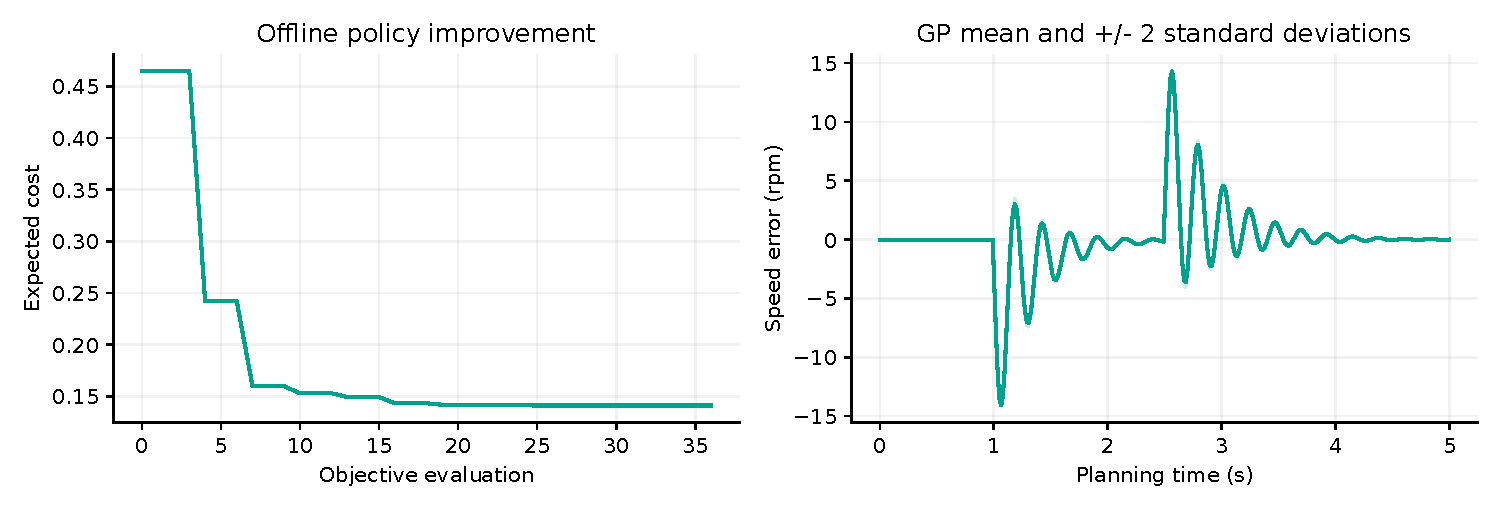
\includegraphics[width=\linewidth,height=.68\textheight,keepaspectratio]{late0_learning.pdf}\caption{Policy-search objective and GP planning response. The shaded interval is model uncertainty, not a certified plant confidence band.}\end{figure}

\subsection{Step 8: nonlinear plant comparison and independent checks}
All three new simulations use the copied T-MATS plant: selected policy at 10\%, selected policy at 5\%, and initial quadratic-feedforward PI at 10\%. Historical traces supply the three earlier comparators. The initial-policy ablation helps distinguish gain learning from merely adding a constant feedforward value. File hashes and replay checks are saved with the study.

\begin{table}[H]\centering\small\begin{tabular}{lrrrr}\toprule Controller & RMSE & Peak & Ringing & Settling\\ & rpm & rpm & lbm/s & s\\\midrule
Base PI & 2.4209 & 21.406 & 2.0702 & 2.475 \\
Original Poly2 + PID & 1.6658 & 14.113 & 1.6968 & 1.365 \\
Retuned Poly2 + PID & 1.5461 & 15.825 & 1.2990 & 0.930 \\
PILCO FF+PI & 1.1973 & 14.389 & 14.8252 & 1.920 \\\bottomrule\end{tabular}\caption{10\% load-amplitude comparison.}\end{table}
\begin{table}[H]\centering\small\begin{tabular}{lrrrr}\toprule Controller & RMSE & Peak & Ringing & Settling\\ & rpm & rpm & lbm/s & s\\\midrule
Base PI & 1.1692 & 10.392 & 1.0583 & 2.115 \\
Original Poly2 + PID & 0.8018 & 6.969 & 0.9005 & 1.260 \\
Retuned Poly2 + PID & 0.7439 & 7.806 & 0.6544 & 0.870 \\
PILCO FF+PI & 0.5930 & 7.008 & 7.9471 & 1.695 \\\bottomrule\end{tabular}\caption{5\% load-amplitude comparison.}\end{table}

RMSE uses every sample in $[60,150]$ s. Peak error is maximum absolute speed error in that interval. IAE uses the same rectangular sample sum as the prior report. Fuel ringing sums, over six two-second event windows, total variation minus absolute net fuel change:
\begin{equation}
 R=\sum_{j=1}^{6}\left[\sum_{k\in W_j}|u_{k+1}-u_k|-|u_{\mathrm{last}(j)}-u_{\mathrm{first}(j)}|\right].
\end{equation}
This is a reversal metric in lbm/s, not fuel consumed. Settling requires persistent entry into $\pm0.1$ rpm until the next event. Numerical acceptance checks full duration, finite signals, positive fuel, positive surge margin, flow residual at most $10^{-9}$, fewer than 200 solver iterations, and pre-test speed within 0.1 rpm.

The analytic GP covariance agrees with a 50,000-input Monte Carlo integration to 0.31\% relative Frobenius error; input/output cross-covariance error is 1.57\%. Held-out one-step speed-increment RMSE ranges from 0.000432 to 0.000709 rpm. Independent command and integral replay errors are below $10^{-8}$. All evaluated new traces pass the existing numerical acceptance checks. The selected 10\% run has minimum surge margin 14.800\% and fuel saturation fraction 0.000\%.
\begin{figure}[H]\centering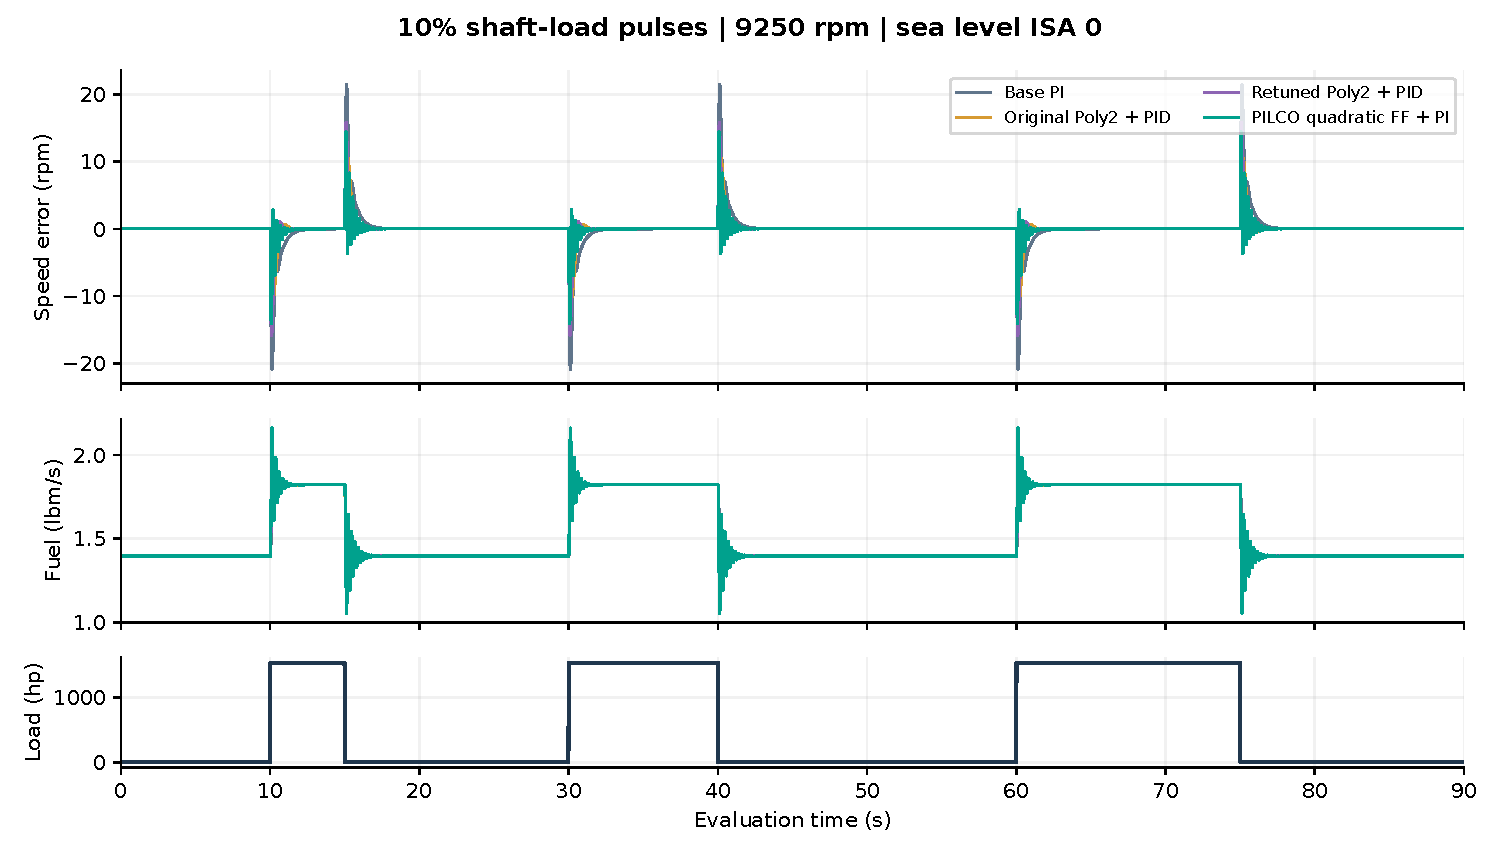
\includegraphics[width=\linewidth,height=.68\textheight,keepaspectratio]{late0_comparison_10pct.pdf}\caption{Full nonlinear 10\% benchmark. Historical methods and new controller use matching time, request and disturbance profiles.}\end{figure}
\begin{figure}[H]\centering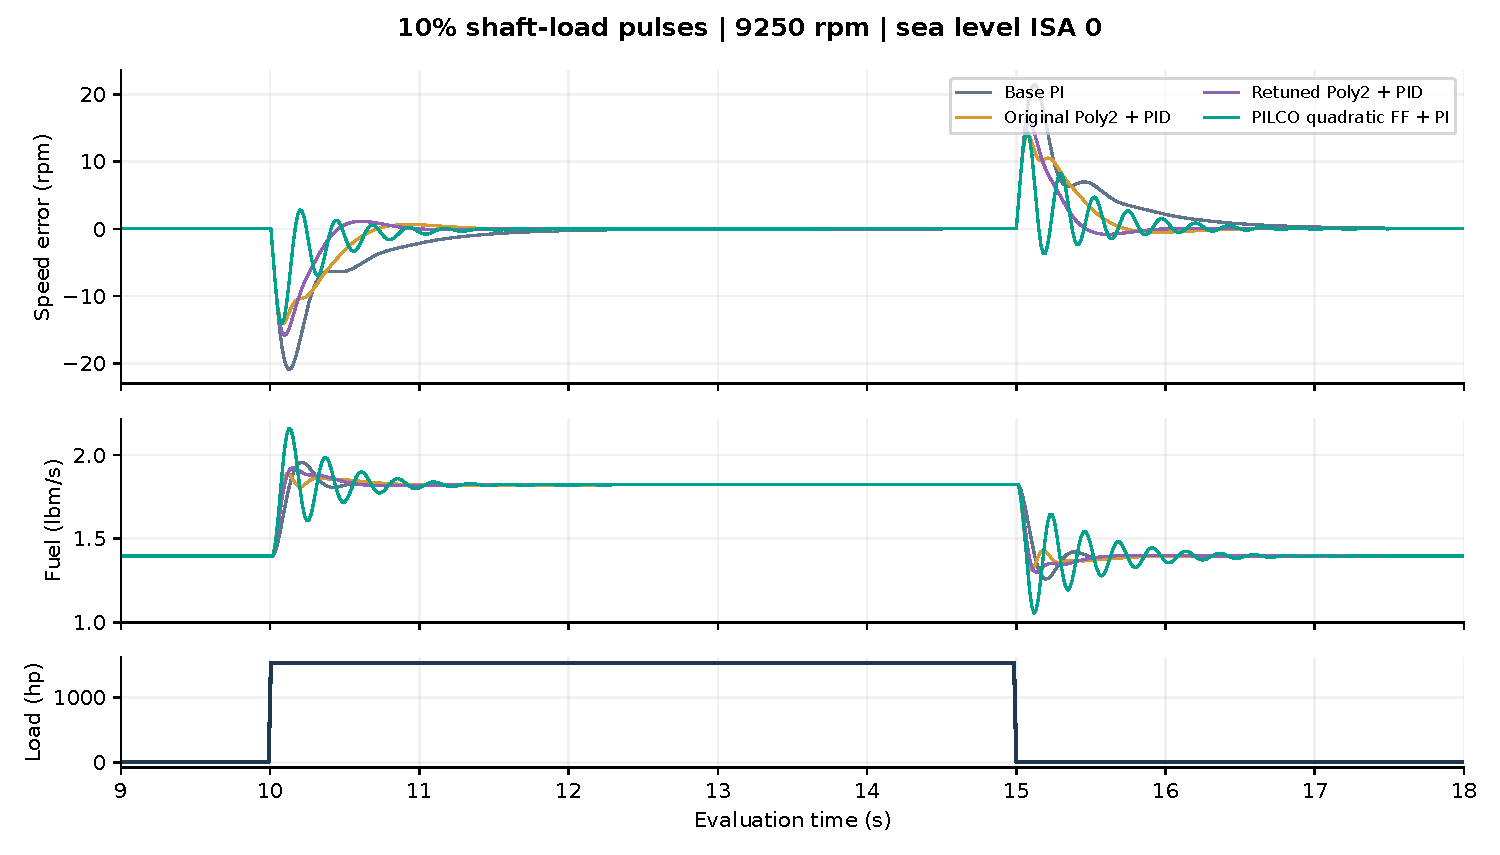
\includegraphics[width=\linewidth,height=.68\textheight,keepaspectratio]{late0_zoom_10pct.pdf}\caption{First pulse, emphasizing overshoot and command reversals. The new method is judged on these plant traces.}\end{figure}
\begin{figure}[H]\centering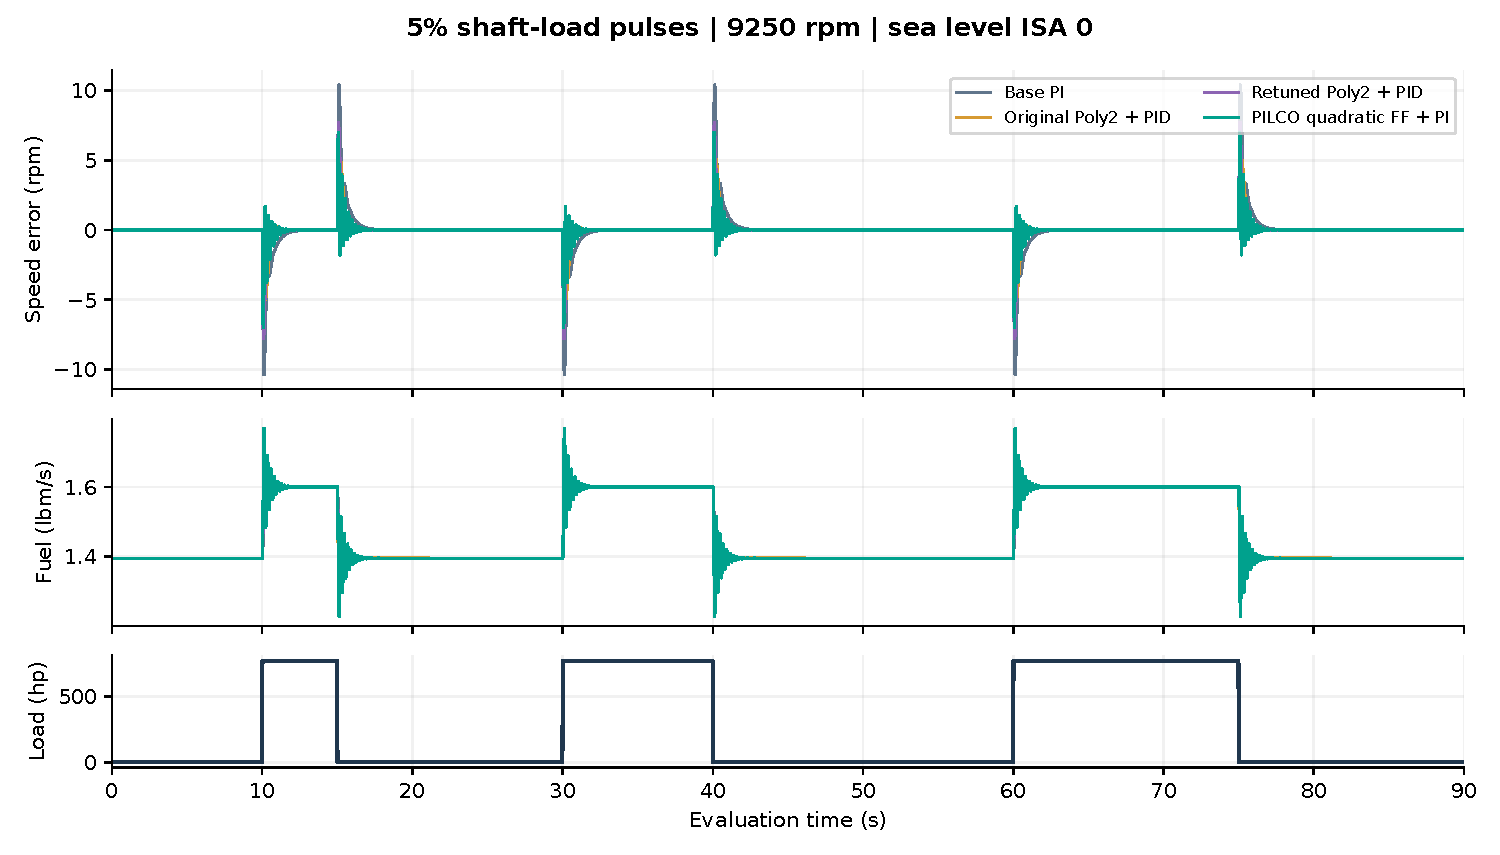
\includegraphics[width=\linewidth,height=.68\textheight,keepaspectratio]{late0_comparison_5pct.pdf}\caption{Frozen-policy 5\% amplitude validation at the same operating point.}\end{figure}

\subsection{Interpretation and limitations}
Relative to Base PI, RMSE changes by -50.5\% and ringing by +616.1\%. Relative to Retuned Poly2 + PID, RMSE changes by -22.6\% and ringing by +1041.2\%. The initial feedforward PI has RMSE 2.4406 rpm and ringing 2.0296 lbm/s. These quantities describe different tradeoffs; minimizing expected tracking cost does not directly minimize fuel reversals.

The original PILCO method uses GP dynamics, uncertainty-aware long-horizon prediction and policy search with analytic gradients~\cite{pilco}. This study retains GP moment matching but changes the policy family, cost, mean function, training source and gradient implementation. It performs one offline improvement round using existing experiments; it does not claim learning from scratch or a repeated collect--refit--improve loop. Forty representative GP points are a subset approximation, and a low held-out one-step error does not establish calibrated long-horizon uncertainty. The moment check validates the algebra against integration, not the physical accuracy of the GP.

The local state omits thermodynamic internal states; the linear mean and GP can absorb only their effects visible in the training trajectories. The deployment sensor dynamics are inherited from the plant, while learning identifies their observed effect. No guarantee of global stability, robustness at other speeds or ambient conditions, or hardware safety follows from these simulations. A multi-speed test with a frozen validation protocol would be required to assess the quadratic feedforward surface itself. The video is an animation of recorded signals; rotor speed is visually scaled and is not a blade-resolved turbine simulation.

\subsection{Reproduction and delivered files}
The source scripts are \path{pilco_tmats.py} (GP and policy learning), \path{tmats_pilco_pi_sfun.m} (deployed controller), \path{tmats_pilco_setup.m}, \path{run_tmats_pilco.m} (plant runs), and \path{build_pilco_deliverables.py} (verification, figures, paper and video). The ready-to-open model is \path{GasTurbine_PILCO_Quadratic_PI.mdl}. It requires the existing adjacent T-MATS library and the frozen fit files in this workspace.

Run Python learning first, then execute \path{run_tmats_pilco} in MATLAB R2018b or a compatible release. Finally run the artifact builder. The results directory contains policy JSON, GP parameters, search history, prediction moments, MAT/CSV plant traces, comparison metrics, replay verification and a hash manifest. The paper source and figures are included alongside the PDF. Re-running overwrites only this study's outputs; preserve them first if a second independent run is desired.



\section{Learning smoother control with an expected ringing penalty}
\textit{Archived October study. All simulations, searches, and checks described below predate this report.}\par

\subsection*{Chapter overview}
The preceding PILCO-style controller reduced speed-error RMSE but produced much larger fuel-command reversals. This study modifies policy learning to penalize expected excess total variation of fuel. A previous-command state and an event-start anchor retain the correlations needed to evaluate that penalty under Gaussian moment propagation. Seven coarse penalty weights and three intermediate refinements are optimized with the unchanged GP dynamics model and checked on the nonlinear gas-turbine plant. A declared joint tracking/ringing score selects a policy using only 10\% load tests, after which a 5\% test evaluates the frozen gains. The method remains an offline PILCO-style adaptation with numerical policy gradients and a frozen quadratic feedforward map. The report separates probabilistic predictions, plant measurements, and limitations.

\subsection{Outcome and why the objective changed}
The selected penalty is $\lambda=0.2$, with $K_p=0.02479762$ and $K_i=0.05385920$. In the nonlinear 10\% test, ringing falls by 85.9\% relative to the previous PILCO policy, from 14.8252 to 2.0838 lbm/s. Speed RMSE changes from 1.1973 to 2.3877 rpm. The smoother command therefore has a measurable tracking cost.

The previous learned gains were $K_p=0.06460568$, $K_i=0.17102610$, $K_d=0$. Their training objective rewarded small speed error and modest fuel magnitude, but neither term distinguished a smooth fuel trajectory from one repeatedly reversing around its equilibrium. A fast, aggressive PI policy could therefore score well despite oscillation. This was visible in the previous full nonlinear 10\% test: RMSE was 1.19728 rpm and ringing was 14.82523 lbm/s, compared with 1.54614 rpm and 1.29904 lbm/s for retuned Poly2 with derivative feedback.

The present change acts in \emph{policy learning}. No post-processing is applied to plant traces or video curves, and no extra low-pass filter is inserted into the fuel command. The deployed controller remains quadratic feedforward plus ordinary speed-error PI; changing its optimized gains changes the actual nonlinear plant response.

\subsection{The experiment and what is held fixed}
The reference is 9250 rpm at sea level, ISA zero and Mach zero. There are 60 s of preparation and 90 s of evaluation at $h=0.015$ s. The three 10\% shaft-load pulses occupy evaluation intervals $[10.005,15)$, $[30,40.005)$ and $[60,75)$ s. Their magnitude is 1537.67919 hp, obtained from the same 15376.79195 hp trim as the preceding studies. Validation uses 768.83960 hp with identical timing. The numerical solver, speed sensor, fuel limits, feedforward coefficients and startup procedure are unchanged.

The dynamics GP is loaded from the previous study without refitting. Its training comprises 4242 transitions from the first two pulse windows of base PI, original Poly2 and retuned Poly2. A 40-point representative subset models residuals around a fitted linear mean. The original third-pulse holdout remains outside GP fitting. However, the 10\% full-test traces now participate in penalty-weight selection; they are tuning results, not independent validation. Five-percent data are never used to choose the policy in this study.

\subsection{Step 1: the deployable controller}
For standardized inverse-model inputs $z_j=(v_j-\bar v_j)/s_j$ with $v=[N,\dot N,T,P]^\top$, retain the full quadratic
\begin{equation}
p_2(v)=c_0+\sum_{j=1}^4c_jz_j+\sum_{j=1}^4c_{jj}z_j^2+\sum_{i<j}c_{ij}z_iz_j.
\end{equation}
At each sample, the actual control law is
\begin{align}
u_{{\rm ff},k}&=p_2(r_k,0,T_k,P_k),& e_k&=r_k-N_{s,k},\\
u_k^*&=u_{{\rm ff},k}+K_pe_k+I_k,&u_k&=\operatorname{clip}(u_k^*,0.2,4),\\
I_{k+1}&=I_k+hK_ie_k&&\text{if conditional integration permits it.}
\end{align}
The integral updates if $(u^*<4\text{ or }e<0)$ and $(u^*>0.2\text{ or }e>0)$, allowing correction out of saturation. Before 45 s, the old command drives the plant and the new integral tracks $I=u_{\rm old}-u_{\rm ff}-K_pe$ for bumpless transfer. Gains have units $(\mathrm{lbm/s})/\mathrm{rpm}$ and $(\mathrm{lbm/s})/(\mathrm{rpm\,s})$.

Only $K_p$ and $K_i$ are learned. The polynomial's fifteen coefficients are fixed. At this single setpoint and ambient condition, feedforward is constant and an integral offset can compensate its value. The experiment therefore assesses PI tuning, not the benefit of the quadratic surface across speeds. The setpoint remains slightly below the old polynomial training-speed minimum of 9264.23 rpm.

\subsection{Step 2: distinguish magnitude, slew, total variation, and ringing}
Fuel magnitude describes how much fuel is commanded. Slew is the local rate $(u_k-u_{k-1})/h$. Total variation counts accumulated command motion, while excess variation removes the unavoidable net motion between endpoints:
\begin{align}
\mathrm{TV}_{a:b}(u)&=\sum_{k=a+1}^{b}|u_k-u_{k-1}|,\\
R_{a:b}(u)&=\mathrm{TV}_{a:b}(u)-|u_b-u_a|\ge0.
\end{align}
The inequality follows from the triangle inequality. For a monotone trajectory $[0,0.5,1]$, TV and net change both equal 1, so ringing is zero. For $[0,1,0,1]$, TV is 3 and net change is 1, so ringing is 2. A direct excess-TV penalty discourages reversals without penalizing a required monotone fuel transition as strongly as plain TV would.

The metric has units lbm/s because it sums changes in a fuel-flow command. It is neither integrated fuel consumption nor the integral of squared fuel slew. It is sensitive to sample rate and noise. This study keeps the sample rate fixed for every comparison. Penalizing ringing does not automatically bound peak slew: the report separately measures that quantity.

\subsection{Step 3: augment the state to preserve temporal correlation}
Use normalized physical and controller states
\begin{equation}
x=\begin{bmatrix}(N-9250)/20\\(N-N_s)/5\\(I-I_0)/0.3\end{bmatrix},\quad
I_0=u_0-u_{\rm ff},\quad\tilde u=\frac{u-u_0}{0.3}=b^\top x,
\end{equation}
where $u_0=1.39529998$ lbm/s and $b^\top=[-20K_p/0.3,\;5K_p/0.3,\;1]$ for the unsaturated fixed-reference policy. To evaluate fuel increments and endpoint changes, introduce
\begin{equation}
\xi=\begin{bmatrix}x\\p\\a\end{bmatrix},\qquad p=\tilde u_{k-1},\qquad a=\tilde u_{\rm event\ start},\qquad
\bar b=\begin{bmatrix}b\\0\\0\end{bmatrix}.
\end{equation}
The five-dimensional covariance includes the cross-covariance between current state, previous command and event-start anchor. Ignoring these correlations would generally overestimate incremental-command uncertainty. In particular,
\begin{equation}
\Var(\tilde u_k-p_k)=\Var(\tilde u_k)+\Var(p_k)-2\Cov(\tilde u_k,p_k).
\end{equation}
At the beginning of each planning event, set the anchor to the current policy output. This is a deterministic linear transformation $\xi\leftarrow T\xi$, where $T$ is identity except its fifth row is $\bar b^\top$. Thus both moments transform: $m\leftarrow Tm$ and $S\leftarrow TST^\top$. Resetting only the anchor mean would be incorrect.

\subsection{Step 4: propagate the unchanged GP and augmented moments}
The normalized GP input is
\begin{equation}
z=[x_1,x_2,\tilde u,d]^\top=B\xi+c(d),\qquad d=P_{\rm load}/1537.6791946.
\end{equation}
With $\xi\sim\mathcal N(m,S)$, its input moments and state/input cross-covariance are $m_z=Bm+c$, $S_z=BSB^\top$, and $C_{\xi z}=SB^\top$. The GP returns two increments $y=[\Delta x_1,\Delta x_2]^\top$. Integration and command memory are known transitions:
\begin{equation}
\xi^+=D\xi+Ey,\qquad
D=\begin{bmatrix}
1&0&0&0&0\\0&1&0&0&0\\-20hK_i/0.3&5hK_i/0.3&1&0&0\\
-20K_p/0.3&5K_p/0.3&1&0&0\\0&0&0&0&1
\end{bmatrix},\qquad E=\begin{bmatrix}1&0\\0&1\\0&0\\0&0\\0&0\end{bmatrix}.
\end{equation}
The fourth state becomes the current command, and the fifth retains the event anchor. The GP residual uses a shared squared-exponential kernel,
\begin{equation}
k(z,z')=\sigma_f^2\exp[-\tfrac12(z-z')^\top\Lambda^{-1}(z-z')],\qquad K_n=K+\sigma_n^2\mathcal I+10^{-9}\mathcal I.
\end{equation}
For Gaussian input, let $q_i=\E[k(z,z_i)]$, $Q_{ij}=\E[k(z,z_i)k(z,z_j)]$ and $\beta=K_n^{-1}R$, where $R$ contains standardized training residuals. Then
\begin{align}
q_i&=\sigma_f^2\frac{|\Lambda|^{1/2}}{|S_z+\Lambda|^{1/2}}
\exp[-\tfrac12(z_i-m_z)^\top(S_z+\Lambda)^{-1}(z_i-m_z)],\\
\mu_g&=\beta^\top q,\\
V_g&=\beta^\top Q\beta-\mu_g\mu_g^\top+
\mathcal I[\sigma_f^2-\operatorname{tr}(K_n^{-1}Q)+\sigma_n^2].
\end{align}
The two-kernel integral $Q$ uses the midpoint $(z_i+z_j)/2$ and covariance $\Lambda/2$; the full expression and previous validation are available in the preceding policy-learning chapter. Restoring residual output scales and the fitted linear mean yields $\mu_y,V_y,C_{\xi y}$. The recursion is
\begin{align}
m^+&=Dm+E\mu_y,\\
S^+&=DSD^\top+EV_yE^\top+DC_{\xi y}E^\top+EC_{\xi y}^\top D^\top.
\end{align}
Each propagated state is approximated as Gaussian. GP noise is treated as independent at successive transitions. This is uncertainty propagation under a model approximation, not a probabilistic safety guarantee or a temporally coherent GP function draw.

\subsection{Step 5: derive expected absolute command motion}
For a scalar Gaussian $Z\sim\mathcal N(\mu,v)$, split the integral at zero:
\begin{align}
\E|Z|&=\int_{-\infty}^0(-z)\mathcal N(z\mid\mu,v)\,dz+
\int_0^\infty z\mathcal N(z\mid\mu,v)\,dz\\
&=\sqrt{\frac{2v}{\pi}}\exp\left(-\frac{\mu^2}{2v}\right)+
\mu\operatorname{erf}\left(\frac{\mu}{\sqrt{2v}}\right)
\equiv F(\mu,v).
\end{align}
For zero variance, take the continuous limit $F(\mu,0)=|\mu|$. For zero mean and positive variance, $F(0,v)=\sqrt{2v/\pi}$, which is nonzero. This exposes why penalizing only $|\E[\Delta u]|$ would miss uncertain command motion.

Define $w_\Delta=\bar b-e_4$ and $w_A=\bar b-e_5$. After a transition,
\begin{align}
\E|\tilde u_k-\tilde u_{k-1}|&=F(w_\Delta^\top m_k,w_\Delta^\top S_kw_\Delta),\\
\E|\tilde u_b-\tilde u_a|&=F(w_A^\top m_b,w_A^\top S_bw_A).
\end{align}
Linearity of expectation permits summing absolute-increment expectations even when increments are correlated. For each event window,
\begin{equation}
\mathcal R_{a:b}=\sum_{k=a+1}^{b}F(w_\Delta^\top m_k,w_\Delta^\top S_kw_\Delta)
-F(w_A^\top m_b,w_A^\top S_bw_A).
\end{equation}
The corresponding physical expected ringing is $0.3\mathcal R$ lbm/s. No extra factor of $h$ belongs in this TV sum: $h\sum |\Delta u/h|=\sum|\Delta u|$. An independent Monte Carlo test checks the folded-normal formula, and a particle rollout cross-checks the complete augmented calculation on the same GP.

\subsection{Step 6: form the objective and search penalty weights}
The former tracking and magnitude costs are retained:
\begin{align}
J_{\rm track}&=h\sum_k(m_{1,k}^2+S_{11,k}),\\
J_{\rm fuel}&=0.01h\sum_k[(\bar b^\top m_k)^2+\bar b^\top S_k\bar b],\\
J_\lambda&=J_{\rm track}+J_{\rm fuel}+\lambda\sum_{\rm events}\mathcal R_{a:b}.
\end{align}
The 5 s planning trajectory applies a unit load for $1\le t<2.5$ s. On the 15 ms grid, transitions begin at 1.005 and 2.505 s. The load-on event closes immediately before unloading, and the unloading event closes at the end of the horizon. Its event windows differ from the fixed two-second windows used in the plant metric. This difference is declared; the plant metric is never replaced by a model prediction.

The coarse weights are $\lambda\in\{0,0.001,0.003,0.01,0.03,0.1,0.3\}$. Candidate zero retains the previous tracking-only gains. Positive weights use bounded L-BFGS-B on $[\log K_p,\log K_i]$, warm-started from the preceding weight. After inspecting the coarse 10\% tradeoff, one refinement adds weights $0.15$, $0.20$ and $0.25$ in the $0.1$--$0.3$ bracket, warm-started from the nearest available weight. This refinement uses tuning data only and is recorded before the added simulations; it does not use 5\% validation. Bounds remain $0.005\le K_p\le0.07$ and $0.01\le K_i\le0.25$. Policy gradients are finite differences of the full probabilistic rollout. This finite set and local optimization do not establish a global optimum.

For each weight, the resulting gains are evaluated in the complete nonlinear 10\% test. The selection score, declared before these evaluations, is
\begin{equation}
S_j=\max\left(\frac{\mathrm{RMSE}_j}{2.4209039065},\frac{R_j}{2.0702280417}\right).
\end{equation}
The denominators are the historical base PI metrics. The smallest score among numerically accepted candidates wins; the score gives equal priority to the worse of these two relative metrics. It does not minimize settling time, peak error, surge margin, or fuel slew. Gains are frozen before 5\% validation.

\begin{table}[H]\centering\small\begin{tabular}{lrrrrr}\toprule
$\lambda$ & $K_p$ & $K_i$ & RMSE & Ringing & Score\\\midrule
0 & 0.06461 & 0.17103 & 1.1973 & 14.8252 & 7.161\\
0.001 & 0.06206 & 0.16260 & 1.2054 & 13.0728 & 6.315\\
0.003 & 0.05751 & 0.15035 & 1.2343 & 10.6050 & 5.123\\
0.01 & 0.04640 & 0.13319 & 1.3609 & 6.8917 & 3.329\\
0.03 & 0.03820 & 0.10339 & 1.5716 & 4.6845 & 2.263\\
0.1 & 0.02949 & 0.07057 & 1.9952 & 2.8858 & 1.394\\
0.15 & 0.02643 & 0.06097 & 2.2146 & 2.3771 & 1.148\\
0.2$^\star$ & 0.02480 & 0.05386 & 2.3877 & 2.0838 & 1.007\\
0.25 & 0.02355 & 0.04890 & 2.5381 & 1.8762 & 1.048\\
0.3 & 0.02216 & 0.04512 & 2.6968 & 1.6841 & 1.114\\\bottomrule\end{tabular}\caption{All tested penalty weights. RMSE is in rpm; ringing is in lbm/s. The star marks the selected policy.}\end{table}
\begin{figure}[H]\centering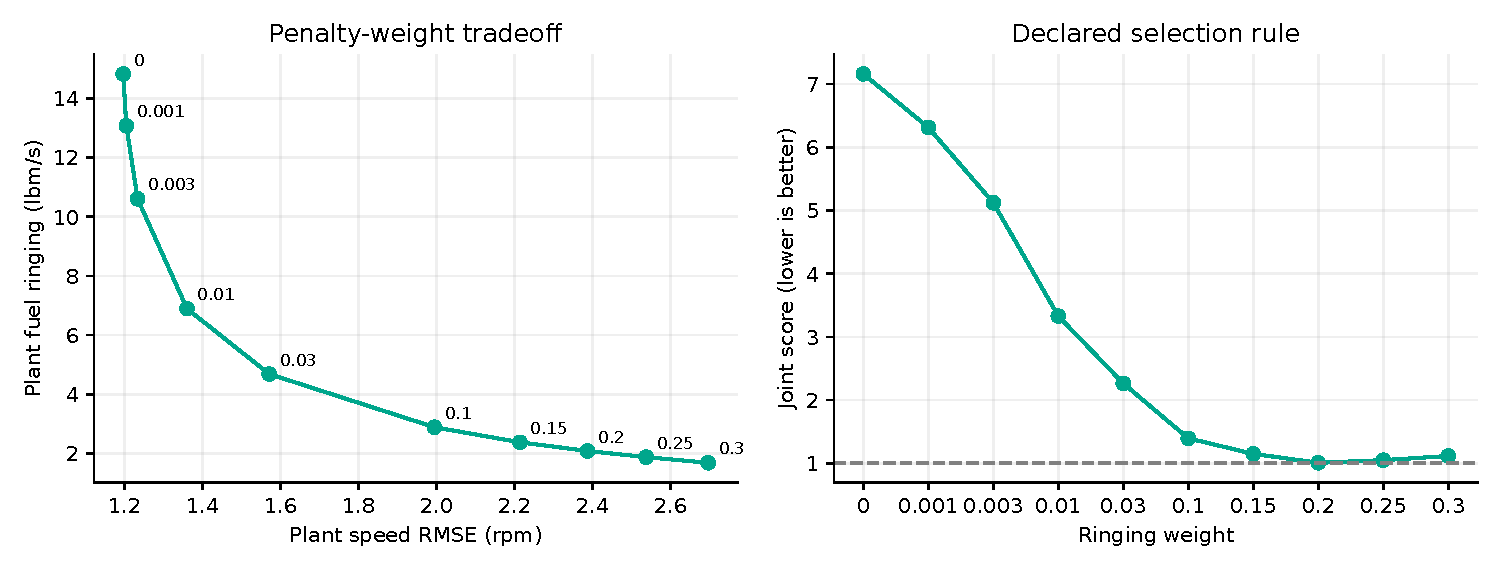
\includegraphics[width=\linewidth,height=.68\textheight,keepaspectratio]{late1_tradeoff.pdf}\caption{Measured 10\% plant tradeoff and the declared selection score. These are candidate evaluations, not independent validation.}\end{figure}

\subsection{Step 7: nonlinear results and interpretation}
The deployed gains are frozen at $K_p=0.02479762$, $K_i=0.05385920$ and $K_d=0$.
\begin{table}[H]\centering\small\begin{tabular}{lrrrr}\toprule
Controller & RMSE (rpm) & Peak (rpm) & Ringing & Settling (s)\\\midrule
Base PI & 2.4209 & 21.406 & 2.0702 & 2.475\\
Original Poly2 & 1.6658 & 14.113 & 1.6968 & 1.365\\
Retuned Poly2 & 1.5461 & 15.825 & 1.2990 & 0.930\\
Previous PILCO & 1.1973 & 14.389 & 14.8252 & 1.920\\
Smooth PILCO & 2.3877 & 21.593 & 2.0838 & 2.220\\\bottomrule\end{tabular}\caption{10\% load test. Ringing units are lbm/s; settling uses the persistent 0.1 rpm band.}\end{table}
\begin{table}[H]\centering\small\begin{tabular}{lrrrr}\toprule
Controller & RMSE (rpm) & Peak (rpm) & Ringing & Settling (s)\\\midrule
Base PI & 1.1692 & 10.392 & 1.0583 & 2.115\\
Original Poly2 & 0.8018 & 6.969 & 0.9005 & 1.260\\
Retuned Poly2 & 0.7439 & 7.806 & 0.6544 & 0.870\\
Previous PILCO & 0.5930 & 7.008 & 7.9471 & 1.695\\
Smooth PILCO & 1.1533 & 10.486 & 1.0615 & 1.905\\\bottomrule\end{tabular}\caption{5\% load test. Ringing units are lbm/s; settling uses the persistent 0.1 rpm band.}\end{table}
Relative to Base PI, smooth PILCO changes RMSE by -1.4\%, ringing by +0.7\%, and fine settling from 2.475 to 2.220 s.

Relative to Retuned Poly2, smooth PILCO changes RMSE by +54.4\%, ringing by +60.4\%, and fine settling from 0.930 to 2.220 s.

Relative to Previous PILCO, smooth PILCO changes RMSE by +99.4\%, ringing by -85.9\%, and fine settling from 1.920 to 2.220 s.

Its sampled peak fuel slew is 4.763 lbm/s$^2$, versus 10.514 for previous PILCO. Minimum surge margin changes from 14.800\% to 18.201\%; the selected 10\% run has 0.000\% fuel saturation. These diagnostics complement the objective rather than entering its selection score.

With the gains frozen, the 5\% test gives RMSE 1.1533 rpm and ringing 1.0615 lbm/s, a 86.6\% ringing reduction from previous PILCO. This supports amplitude transfer of the smoothing effect at this operating point.

\paragraph{What the video compares.} Four synchronized windows show base PI, retuned Poly2 + PID, previous PILCO, and smooth PILCO. Original Poly2 remains in the report tables but is omitted from the four-window video to make room for the new method. Each window has its own speed-error and fuel plots, matching axes, current speed, current fuel, a shaft-load indicator and full-test metrics. Orange shading marks load-on intervals. The video includes the full 10\% test, slowed load application/removal, frozen-gain 5\% validation and a final scorecard. All plotted values are recorded plant signals without visual smoothing.

\begin{figure}[H]\centering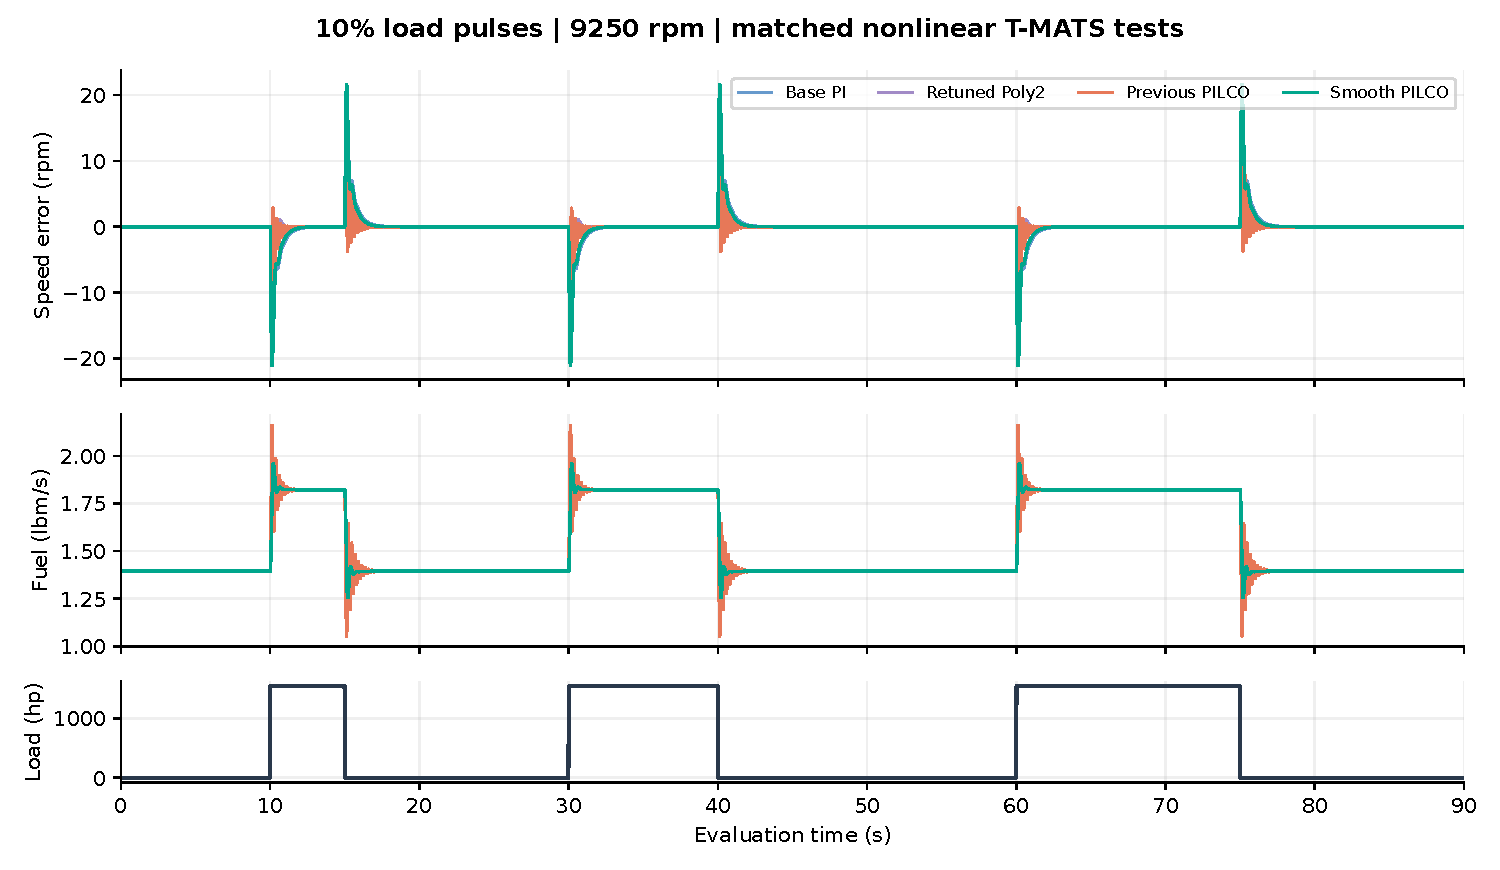
\includegraphics[width=\linewidth,height=.68\textheight,keepaspectratio]{late1_full_comparison.pdf}\caption{10\% full test; only the controller gains differ between the two PILCO policies.}\end{figure}
\begin{figure}[H]\centering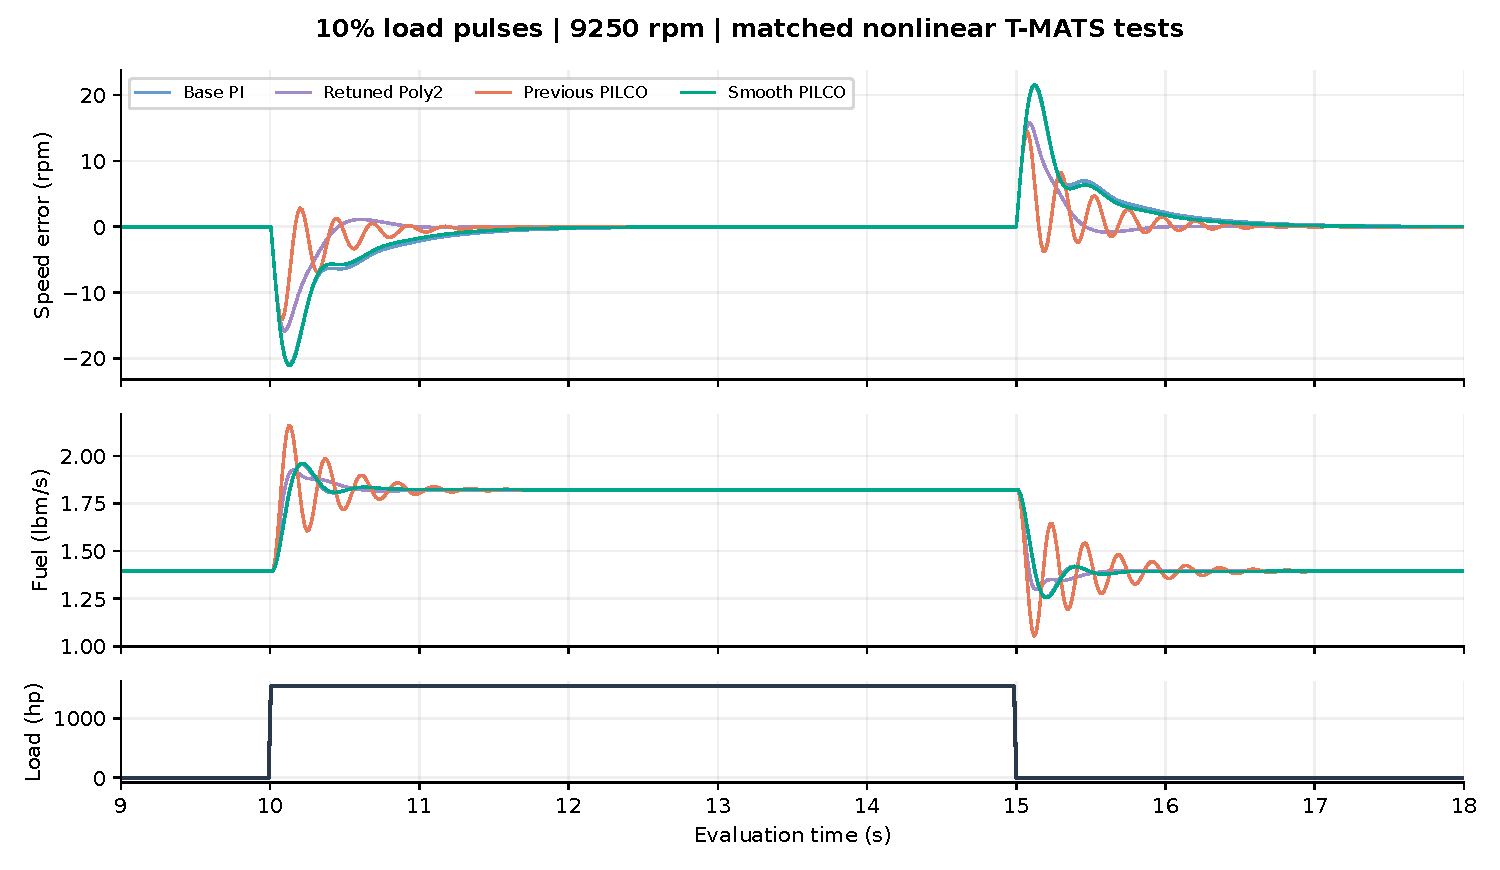
\includegraphics[width=\linewidth,height=.68\textheight,keepaspectratio]{late1_zoom_comparison.pdf}\caption{First load pulse, showing the effect of the ringing penalty on physical speed and fuel command.}\end{figure}
\begin{figure}[H]\centering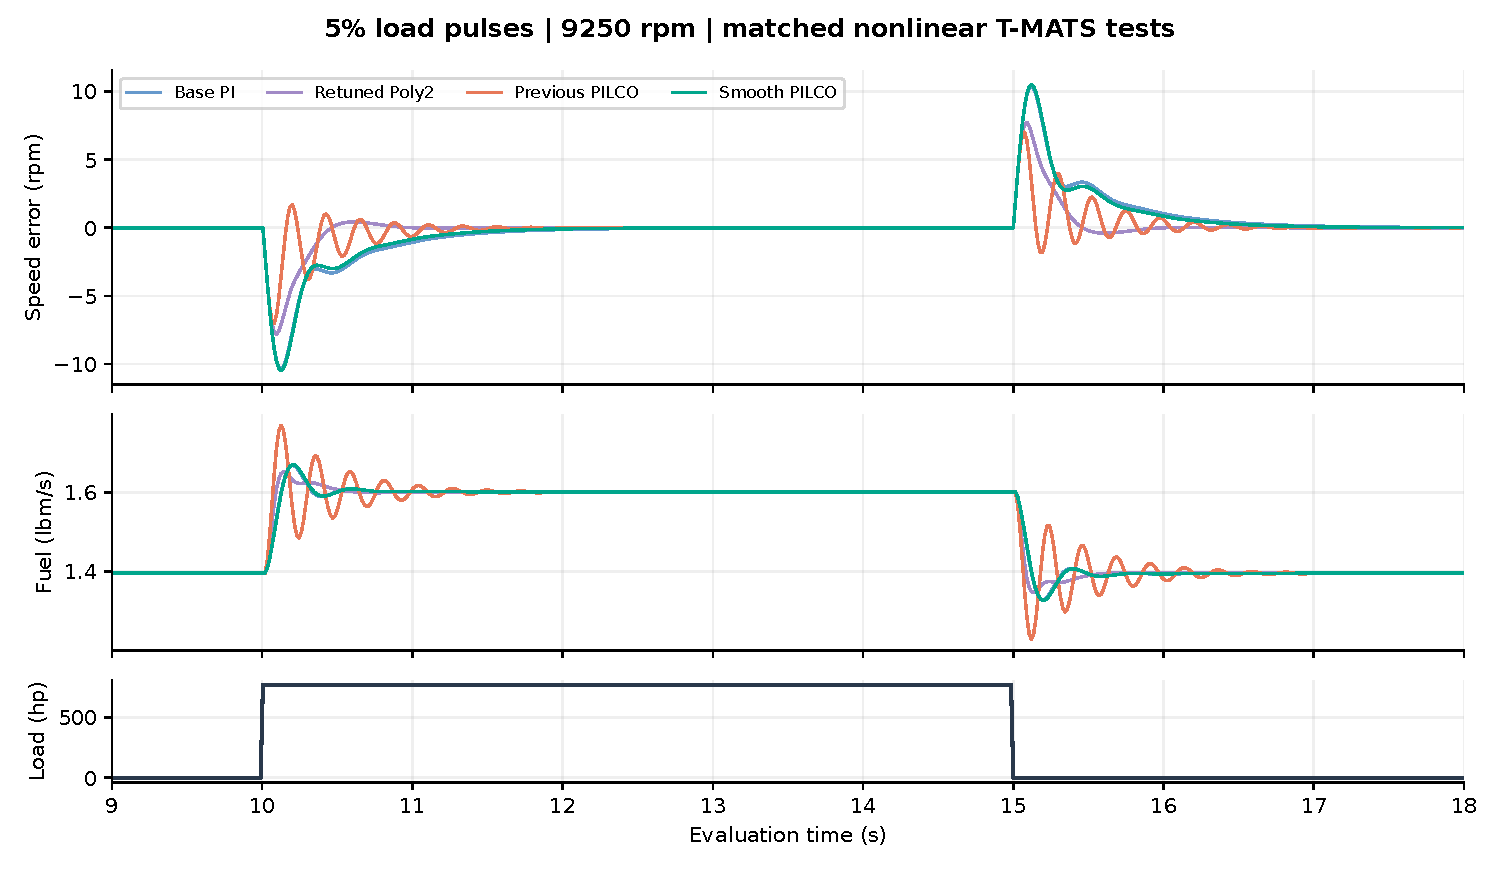
\includegraphics[width=\linewidth,height=.68\textheight,keepaspectratio]{late1_validation_comparison.pdf}\caption{Frozen-policy 5\% amplitude validation with the same timing and plant.}\end{figure}
\begin{figure}[H]\centering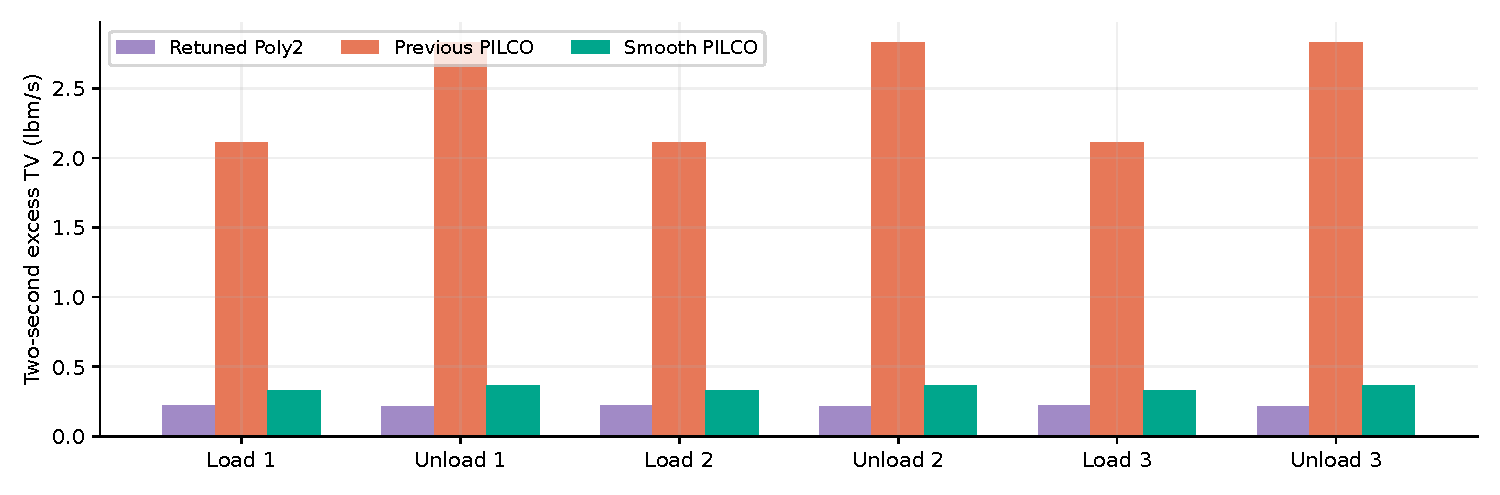
\includegraphics[width=\linewidth,height=.68\textheight,keepaspectratio]{late1_event_ringing.pdf}\caption{Ringing decomposed into six individual 10\% load edges. Each bar is total fuel movement minus net movement in the same two-second window.}\end{figure}

\subsection{Step 8: numerical checks and metric definitions}
All selected traces pass the shared plant acceptance checks. Maximum independent command replay discrepancy is 1.46e-13 lbm/s; maximum integral update discrepancy is 5.38e-15 lbm/s. The folded-normal formula passes 250,000-sample scalar Monte Carlo checks, including zero-variance and nonzero-variance cases. For the selected policy, a 5000-particle GP rollout predicts normalized excess TV 2.317963, compared with 2.317930 from Gaussian moment closure; their relative difference is 0.0014\%. The particle standard error is 0.000037. This checks prediction consistency on the same surrogate; it does not independently validate the physical GP uncertainty.

The plant acceptance test requires finite signals, positive fuel, positive surge margin, flow residual at most $10^{-9}$, fewer than 200 solver iterations, full 150 s duration and preparation speed within 0.1 rpm. Speed RMSE and peak error use all evaluation samples. IAE uses the previous study's rectangular sum. Ringing sums TV minus endpoint motion in six two-second load-edge windows. Fine settling requires staying inside $\pm0.1$ rpm until the next event; it is not a broad percentage-of-speed settling criterion. Reported peak slew is the maximum sampled fuel change divided by 0.015 s in those windows.

Independent replay reconstructs $u^*=u_{\rm ff}+K_p(r-N_s)+I$ and every eligible integral update, then checks the saved command. Metrics are recomputed from CSV and compared against MATLAB's shared implementation. Identical time, reference and load vectors are checked across compared runs. The extra previous-command and anchor states exist only in offline prediction: the runtime controller still requires just its integral state.

\subsection{Limits and how to use the result}
The result is smoother than the earlier tracking-only PILCO, but the complete comparison must also account for tracking, settling and surge margin. It does not dominate the retuned Poly2 controller on both speed RMSE and ringing. That comparator has derivative/acceleration feedback, whereas the new policy is restricted to PI. The chosen weight is the best under the declared score among the tested candidates, not a universal tuning value.

This is an offline PILCO-style method, not a reproduction of the original full collect--refit--improve loop. The original PILCO work motivates GP dynamics and uncertainty-aware policy evaluation~\cite{pilco}. This implementation uses a fitted linear mean, a subset GP with shared covariance hyperparameters, a restricted PI policy, numerical gradients, and a custom expected excess-TV cost. It assumes an unsaturated affine policy during planning; plant runs apply the actual saturation and anti-windup. Five-percent testing checks amplitude transfer at one operating point and is not proof of robustness to noise, speed changes, ambient changes or hardware dynamics.

To prioritize still less actuator activity, select a larger penalty only after examining its tracking cost. To require a hard slew bound, add and validate an explicit actuator-rate constraint or a different policy architecture; an excess-TV penalty alone does not provide such a bound. To claim advantages for the quadratic feedforward map itself, perform separate multi-speed and ambient validation.

\subsection{Reproduction}
Run \path{pilco_smooth.py} to load the frozen GP and optimize the coarse weights. Run \path{run_tmats_pilco_smooth('tune')} in MATLAB. Run \path{refine_pilco_smooth.py}, then repeat the MATLAB tuning call, which resumes saved candidates and evaluates the additions. Run \path{select_pilco_smooth.py} to write \path{selected_policy.json}, then \path{run_tmats_pilco_smooth('validate')} only after selection. The ready-to-open model is \path{GasTurbine_PILCO_Smooth_PI.mdl}; its preload callback loads the frozen selected policy. Run \path{check_pilco_smooth_mc.py} for the particle cross-check and the report/video builders for final artifacts. Outputs are in \path{results/pilco_smooth_20261010}. This is an overlay for the existing T-MATS workspace and adjacent library; earlier studies remain unchanged.




\chapter{Frozen-controller acceleration and the combined cycle}
\label{ch:transfer}
These tests change the operating task after the earlier local controller development. The no-load ramp and common-sensor audit distinguish actual mechanical speed from the feedback measurement. The first combined cycle is a transfer test for the earlier frozen controllers; the same cycle later becomes a selection case for DOB98. Its evidential role therefore depends on the controller being discussed.

\section{Five-second no-load acceleration and the common-sensor audit}
\textit{Archived October study. All simulations, searches, and checks described below predate this report.}\par

\subsection*{Chapter overview}Four existing controllers are tested on the same nonlinear plant with zero external shaft extraction. The target rises from 9000 to 10000 rpm in five seconds. Base PI has the lowest ramp tracking error in this experiment. Ringing-aware PILCO improves ramp tracking relative to the previous PILCO, but does not outperform base PI. This is a transfer test of frozen policies, not a new training result.
\subsection{Identical-sensor audit and fresh rerun}
All four models explicitly use the same T-MATS first-order speed-sensor library block: time constant 0.05 s, unity gain, limits 0--20000 rpm, initial value from the same plant initial speed, noise disabled, unity fault gain and zero drift. The sensor sample-time setting is the same plant solve interval. Model wiring assertions verify that both the base PI and each active advanced controller receive this sensor output directly. The sensor input comes from the same plant-output block in every model.

The earlier models already had these settings. The new simulations explicitly enforce them in separate model copies and reproduce the earlier speed, sensed-speed and fuel traces. Thus the prior ranking was not caused by unequal sensor dynamics. Controllers respond differently to the same lag. During a ramp, actual-speed error and sensed-speed error differ; the primary tables continue to score actual shaft speed. Individual audit JSON files and a sensor-comparison CSV accompany the results.
\subsection{Reproducible test protocol}
Rated speed is defined as $N_{100}=10000$ rpm. With $\tau=t-60$ s, the reference is
\begin{equation}r(\tau)=9000+200\min\{5,\max\{0,\tau\}\}\quad\text{rpm}.\end{equation}
Thus the reference acceleration is $200$ rpm/s, or two percentage points of rated speed per second. External PTO load is identically zero. The compressor still consumes shaft power: no external load does not mean zero internal torque.

The plant starts at 10000 rpm, ramps down during absolute time 5--10 s, and settles at 9000 rpm before the evaluation begins at 60 s. Controller handover is at 45 s. All four traces are within 0.1 rpm of 9000 rpm throughout the final five seconds before the test. The requested acceleration occurs at absolute time 60--65 s; simulation continues to 80.01 s. Sea-level, ISA-zero, Mach-zero settings are shared. The reference governor permits 200 rpm/s.

Logged samples are spaced by 0.015 s. The continuous target ramp lasts exactly 5 s; its first post-end sample is at $\tau=5.01$ s. Maximum logged-reference discrepancy from the equation above is below $2\times10^{-12}$ rpm. Every saved sample passes the existing model-validity flag, and every external-load sample is zero.

\subsection{Controllers held fixed}
\begin{center}\small\begin{tabular}{lrrr}\toprule Controller & $K_p$ & $K_i$ & $K_d$\\\midrule
Base PI & .025 & .050 & 0\\
Retuned Poly2 + PID & .025 & .140 & .00125\\
Previous PILCO & .06460568 & .17102610 & 0\\
Smooth PILCO & .02479762 & .05385920 & 0\\\bottomrule\end{tabular}\end{center}
Both PILCO-style policies retain the prior quadratic feedforward, PI feedback, saturation and anti-windup implementation. Their nominal command structure is
\begin{align}u_k^*&=p_2(r_k,0,T_k,P_k)+K_p(r_k-N_{s,k})+I_k,\\
u_k&=\operatorname{clip}(u_k^*,0.2,4.0),\qquad
I_{k+1}=I_k+hK_i(r_k-N_{s,k}),\end{align}
with conditional integration at saturation. The zero second feedforward argument is retained from the prior controller, including during acceleration. No acceleration feedforward term is newly fitted for this test. The Poly2 PID comparator retains its previous inverse-model/derivative implementation; it is not replaced by the PILCO PI law.
\subsection{Measured response}
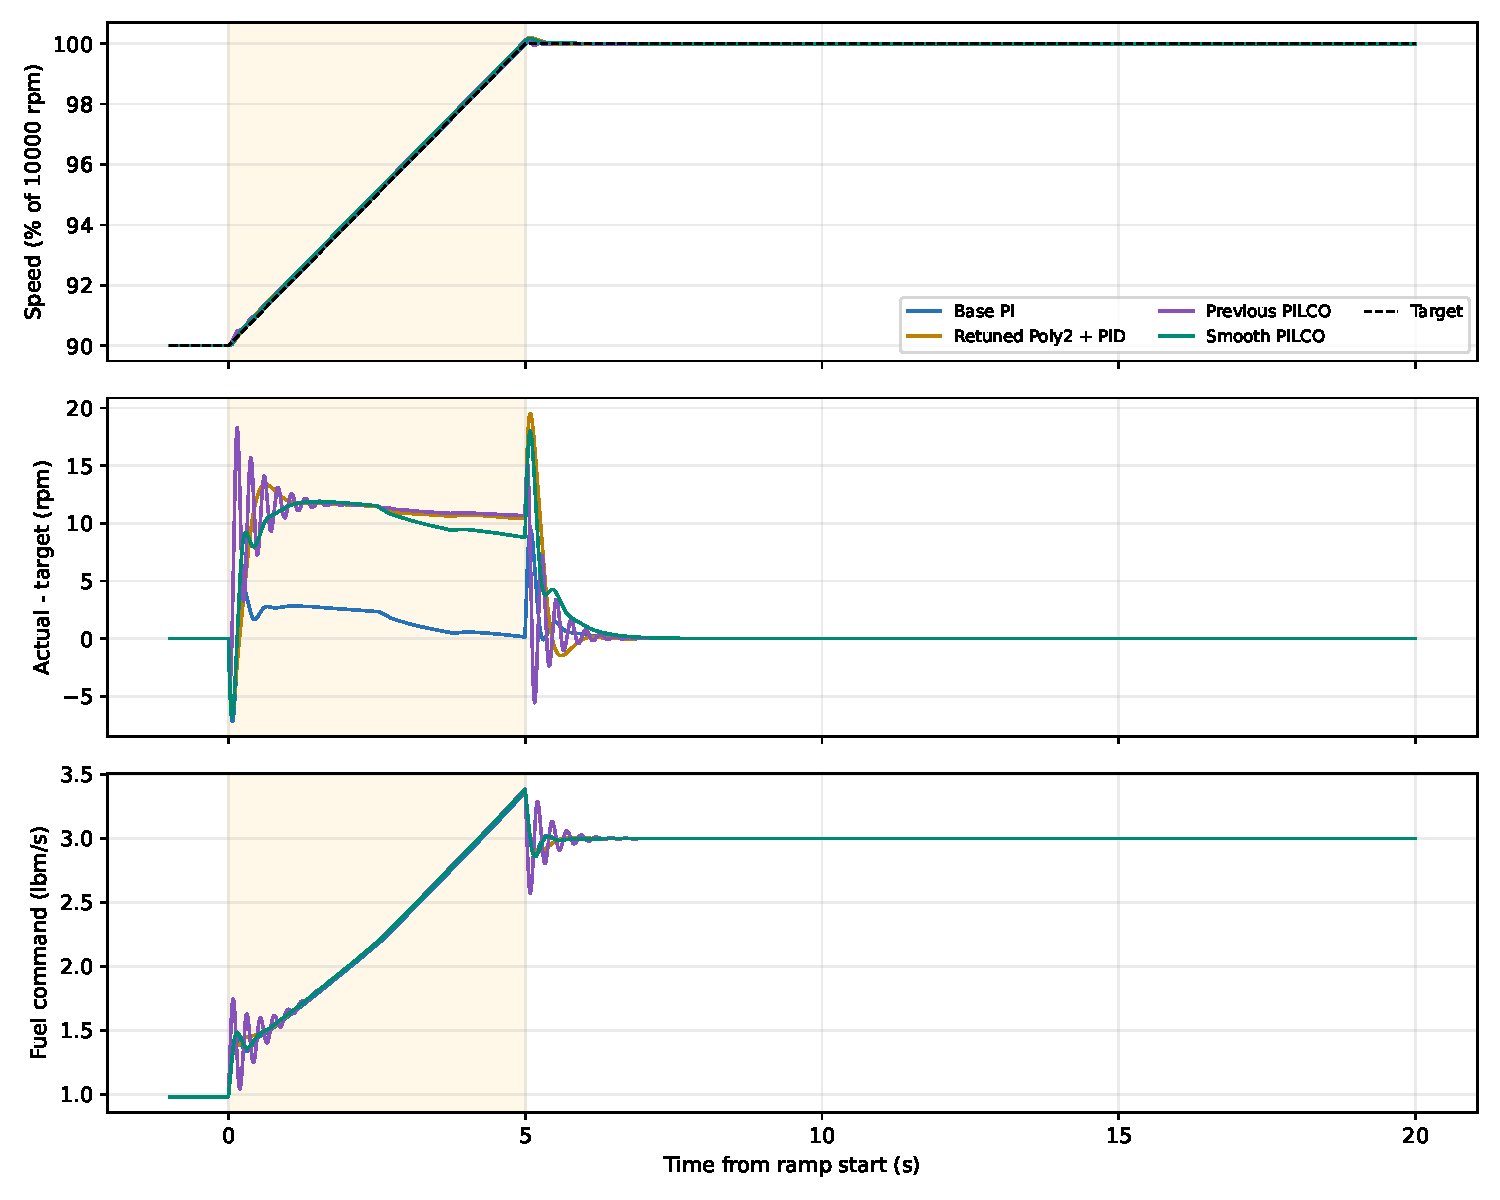
\includegraphics[width=\textwidth,height=.68\textheight,keepaspectratio]{late2_responses.pdf}
The pale band marks the five-second target ramp. Curves are raw recorded simulation traces; no display smoothing is used. Speed curves nearly overlap at the full-speed scale, so the signed error panel is needed to distinguish tracking performance.
\subsection{Quantitative comparison}
For each sample, $e_k=N_k-r_k$. Ramp RMSE uses $0\leq\tau<5$ s; full RMSE uses $0\leq\tau\leq20.01$ s. Settling is measured after ramp completion: the first recorded time after which every remaining sample stays within $\pm1$ rpm of 10000 rpm, minus 5 s. It is a finite-record measurement.
\begin{center}\small\begin{tabular}{lrrrr}\toprule
Controller & Ramp RMSE & Full RMSE & Peak $|e|$ & Settle\\
 & rpm & rpm & rpm & s after ramp\\\midrule
Base PI & 2.161 & 1.309 & 9.42 & 0.610 \\
Retuned Poly2 + PID & 10.949 & 5.799 & 19.54 & 0.760 \\
Previous PILCO & 11.224 & 5.710 & 18.31 & 0.820 \\
Smooth PILCO & 10.252 & 5.392 & 18.00 & 1.045 \\
\bottomrule\end{tabular}\end{center}
Fuel excess total variation is
\begin{equation}R_u=\sum_{k=a+1}^{b}|u_k-u_{k-1}|-|u_b-u_a|.\end{equation}
It measures movement beyond net endpoint change, in lbm/s, not fuel consumption. For acceleration, some excess variation is physically useful: fuel may rise to accelerate and then drop to its steady value. Therefore the whole-test measure is not a pure measure of unwanted oscillation. A separate post-ramp value is included. These intervals differ from the earlier load-pulse study; their totals must not be compared directly.
\begin{center}\small\begin{tabular}{lrrrr}\toprule
Controller & Whole $R_u$ & Post-ramp $R_u$ & Overshoot & Min. surge\\
 & lbm/s & lbm/s & rpm & \%\\\midrule
Base PI & 1.2188 & 0.2895 & 9.42 & 13.98 \\
Retuned Poly2 + PID & 1.0004 & 0.2189 & 19.54 & 13.74 \\
Previous PILCO & 6.2413 & 2.6423 & 15.23 & 13.74 \\
Smooth PILCO & 1.3489 & 0.3454 & 18.00 & 13.78 \\
\bottomrule\end{tabular}\end{center}
\subsection{Interpretation and limits}
Base PI gives the smallest ramp and full-evaluation RMSE. The smooth PILCO ramp RMSE is 10.252 rpm versus 11.224 rpm for the previous PILCO, an 8.7\% reduction. This does not establish a universal ranking: the earlier load-disturbance objective and the present acceleration objective are different.

PILCO gains were learned around 9250 rpm under load pulses. This ramp moves beyond that local operating condition; portions also lie beyond the approximately 9264--9750 rpm polynomial fitting range. The present result is evidence for this single deterministic nominal simulation, not a robustness guarantee. It does not validate the Gaussian-process model across the entire ramp or prove that a ringing penalty alone explains all differences between the gain sets.

The previous derivation remains applicable to how the gains were obtained: expected tracking and fuel-magnitude costs were augmented by expected excess fuel variation, using previous-command and segment-anchor memory. This run does not retrain that objective. A dedicated acceleration-training study would be needed to claim optimized ramp performance.
\subsection{Reproduction}
Run \path{ramp90_equal_sensor_batch.m} in MATLAB with the existing T-MATS dependencies. The four \path{GasTurbine_EqualSensor_*.mdl} copies preserve previous studies. Raw CSV/MAT traces and summary metrics are in \path{results/pilco_ramp90_equal_sensor_20261010}. Run \path{build_ramp90_equal_sensor.py} for this analysis and \path{build_ramp90_equal_sensor.py} for the synchronized video.


\section{Combined acceleration and a five-second load pulse}
\textit{Archived October study. All simulations, searches, and checks described below predate this report.}\par

\subsection{Requested cycle}
Define relative time $\tau=t-60$ s. The shaft-speed target and external load are
\begin{align}
r(\tau)&=9000+200\min(5,\max(0,\tau))\quad\mathrm{rpm},\\
P_L(\tau)&=\begin{cases}0.1P_{\rm ref},&10\le\tau<15,\\0,&\text{otherwise}.\end{cases}
\end{align}
The speed target ramps from 90\% to 100\% in five seconds, then remains at 10000 rpm. A common load is applied at second 10 and removed at second 15. Recovery is recorded through second 25.005. The five-second pulse is programmed as a zero-order-held workspace signal, with interpolation disabled.

The reference is the mean turbine shaft power at settled 10000 rpm from seconds 8--10 of the preceding no-load base-PI run: $P_{\rm ref}=27896.501$ hp. Therefore every controller receives exactly the same pulse amplitude, 2789.650 hp. This is 10\% of that common turbine-power reference, not 10\% of each controller's instantaneous power. Internal compressor power is still present.

The preparation stage begins at 10000 rpm, moves to 9000 rpm during absolute seconds 5--10, and settles before the cycle starts at absolute second 60. All cases use sea-level ISA-zero, Mach-zero conditions. Controller gains remain fixed. All four sensors have a 0.05 s time constant, unity gain, identical limits and initial conditions, and noise disabled. Wiring assertions confirm that each active controller receives the sensor output.

The model sample interval is 0.015 s. The first logged loaded sample is at relative 10.005 s, and the first unloaded sample is at 15.000 s. The programmed event interval is exactly 10--15 s; observed event timing is resolved on the sample grid. All simulations pass the existing model-validity checks.
\subsection{Comparison definitions}
Error means actual shaft speed minus target, $e_k=N_k-r_k$. Ramp RMSE uses $0\le\tau<5$ s; load/recovery RMSE uses $10\le\tau\le25.005$ s; full-cycle RMSE uses $0\le\tau\le25.005$ s. These are sample-weighted metrics. Scoring the two phases separately prevents the long recovery interval from concealing ramp differences.
\subsection{Recorded responses}
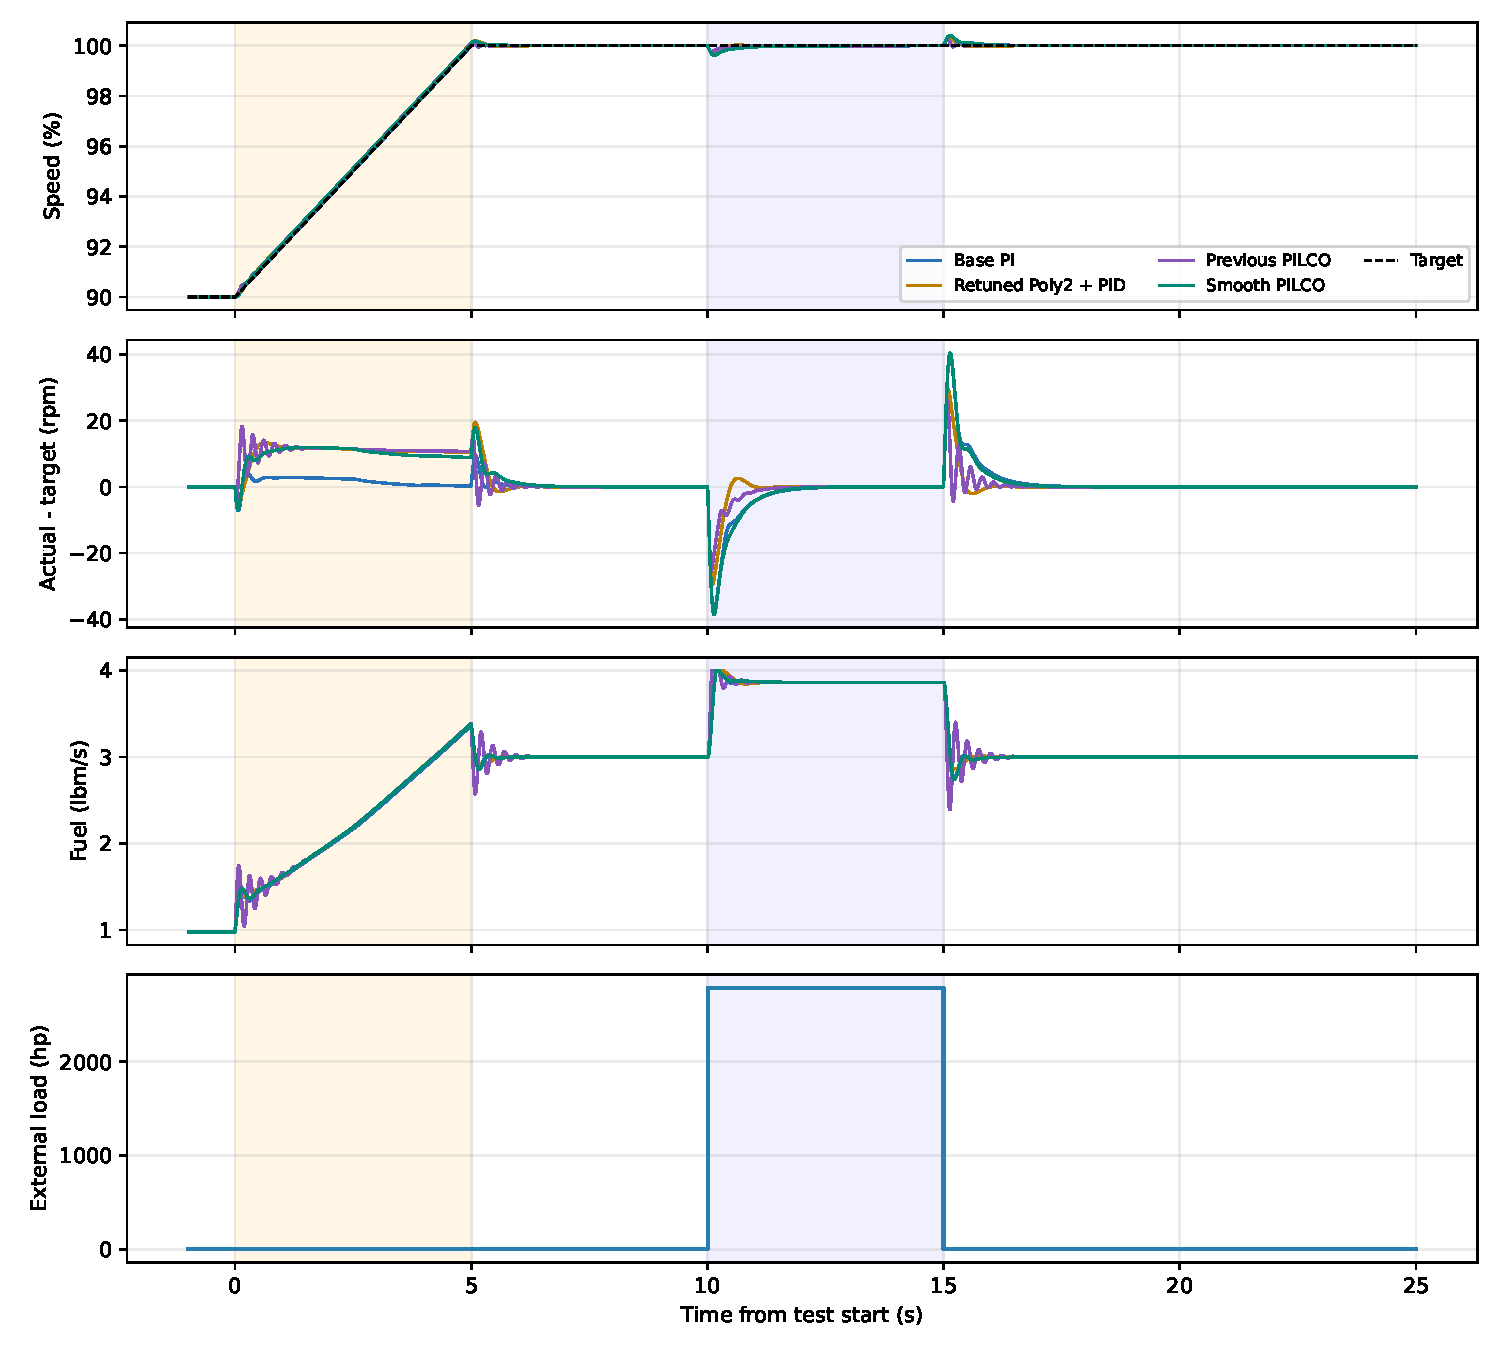
\includegraphics[width=\textwidth,height=.68\textheight,keepaspectratio]{late3_responses.pdf}
Orange shading marks the target ramp; blue shading marks the external-load pulse. These are raw nonlinear simulation traces, with no visual smoothing.
\subsection{Numerical results}
\begin{center}\small\begin{tabular}{lrrr}\toprule
Controller & Ramp RMSE & Load/recovery RMSE & Full RMSE\\ & rpm & rpm & rpm\\\midrule
Base PI & 2.161 & 6.815 & 5.408 \\
Retuned Poly2 + PID & 10.949 & 4.416 & 6.214 \\
Previous PILCO & 11.224 & 3.393 & 5.745 \\
Smooth PILCO & 10.252 & 6.913 & 7.207 \\
\bottomrule\end{tabular}\end{center}
\begin{center}\small\begin{tabular}{lrrrr}\toprule
Controller & Load peak $|e|$ & Fuel excess TV & Min. surge & Saturation\\
& rpm & lbm/s & \% & \% samples\\\midrule
Base PI & 40.13 & 0.945 & 7.64 & 0.7 \\
Retuned Poly2 + PID & 29.39 & 0.696 & 7.75 & 0.1 \\
Previous PILCO & 26.03 & 4.489 & 7.77 & 0.7 \\
Smooth PILCO & 40.47 & 0.919 & 7.63 & 0.2 \\
\bottomrule\end{tabular}\end{center}
Fuel excess total variation is $\sum|\Delta u|-|u_{\rm end}-u_{\rm start}|$, computed separately over 10--15 s and 15--25.005 s and then summed. It describes excess command movement, not fuel consumption. Minimum surge margin and fuel saturation are evaluated over the full cycle.

The previous and smooth PILCO policies use quadratic setpoint feedforward plus PI feedback. Retuned Poly2 retains its inverse-model/PID implementation; base PI remains the original baseline. No gains, feedforward coefficients or ringing weights were fitted to this combined cycle. These are nominal transfer-test results, not proof of robustness or global superiority. In particular, all controllers share the same sensor dynamics; differences in actual-speed tracking must not be attributed to unequal sensor time constants.
\subsection{Reproduction and saved outputs}
Run \path{combined_cycle_batch.m} in the existing MATLAB/T-MATS workspace. New models are named \path{GasTurbine_Combined_*.mdl}; earlier studies are preserved. Raw traces, model audit JSON, numerical metrics and the exact protocol are saved under \path{results/pilco_combined_cycle_20261010}. Analysis and video builders are \path{build_combined_cycle.py} and \path{build_combined_video.py}.



\chapter{Local DOB98 design, PI retuning, and attribution}
\label{ch:dob98}
The observer is identified around a physical speed of 9800 rpm; the number 98 does not describe model-fit accuracy. The independent multisine assesses the local predictor. The combined ramp/load cycle selects PI gains with the observer enabled and must be reported as selection evidence. The original-gain observer result is retained as a partial attribution check.

\section{A new inverse model at 9800 rpm and PI tuning after DOB engagement}
\textit{Archived October study. All simulations, searches, and checks described below predate this report.}\par

\subsection{Scope and identification experiment}
Previous PILCO is replaced in this comparison by DOB98 + tuned PI. Base PI, retuned Poly2 + PID and smooth PILCO retain their earlier gains and traces. The new controller uses no quadratic feedforward. Its structure is PI minus a filtered input-disturbance estimate, followed by the common fuel limits.

A new nominal model is identified specifically at 9800 rpm (98\% rated speed), with zero external shaft load. After preparation, training applies a deterministic binary fuel perturbation of amplitude 0.035 lbm/s, switched approximately every 0.18 s for 30 s. The base PI stabilizes the experiment; identification uses actual applied fuel, including the excitation, and actual shaft speed. Independent validation uses the sum of 0.37 and 1.17 Hz sinusoids, with amplitudes 0.025 and 0.015 lbm/s. No validation samples enter the least-squares fit.

Let $y_k=N_k-9800$ and $v_k=u_k-u_0$, with $u_0=2.530351198$ lbm/s and $T_s=0.015$ s. A parsimonious local model is
\begin{equation}y_{k+1}=a y_k+b v_k,\qquad
a=0.9789097769,\quad b=9.3039586704.\end{equation}
The parameters minimize the squared one-step residual over the excited training interval. The identified pole is stable, and the numerator has no finite nonminimum-phase zero. The model is local: the training speed varies only a few rpm around 9800. Independent free-run fit is 99.7829\%, with 0.001406 rpm RMSE. Fit means $100(1-\|y-\hat y\|/\|y-\bar y\|)$.
\par\noindent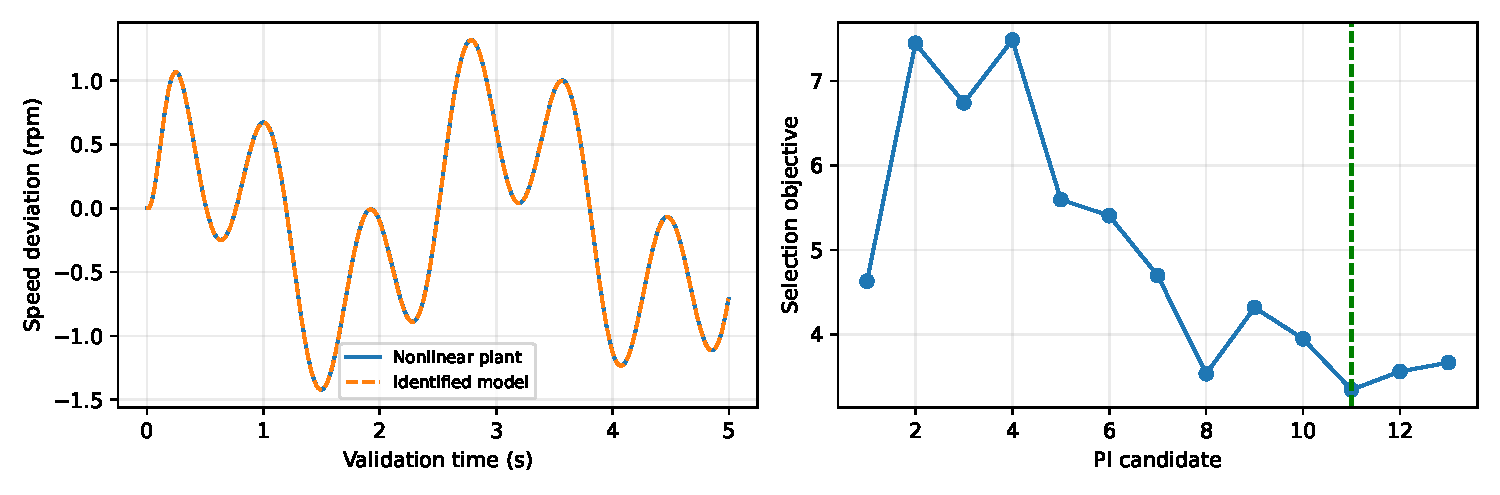
\includegraphics[width=\textwidth,height=.68\textheight,keepaspectratio]{late4_identification_tuning.pdf}
\subsection{Causal filtered inverse, step by step}
\textbf{1. Nominal speed dynamics.} With $q=z^{-1}$ denoting a one-sample delay,
\begin{equation}P_n(q)=\frac{bq}{1-aq}.\end{equation}
\textbf{2. Include the sensor.} Every controller retains the same physical sensor: time constant 0.05 s, unity gain, common initial conditions and noise disabled. The DOB uses its discrete approximation
\begin{equation}H_n(q)=\frac{(1-p)q}{1-pq},\qquad p=e^{-T_s/0.05}.\end{equation}
Thus the inverse is formed for sensed-speed dynamics $P_nH_n$. This approximation does not change the physical sensor blocks.

\textbf{3. Make the inverse causal and filtered.} Choose a unity-DC, two-pole low-pass filter with two delays:
\begin{equation}Q(q)=\frac{(1-r)^2q^2}{(1-rq)^2},\qquad r=e^{-2\pi f_cT_s},\quad f_c=1\ \mathrm{Hz}.\end{equation}
Then the two nominal delays cancel analytically:
\begin{equation}\frac{Q}{P_nH_n}=\frac{(1-r)^2(1-aq)(1-pq)}{b(1-p)(1-rq)^2}.\end{equation}
This is proper, causal and stable. A numerical frequency-response check verifies the identity, and an independent Python filter replay is compared with the recorded Simulink observer output.

\textbf{4. Estimate input-equivalent disturbance.} Use the known saturated command, without access to the external load signal:
\begin{equation}\hat d_{\rm raw}=\frac{Q}{P_nH_n}(N_s-N_0)-Q(u_{\rm cmd}-u_0).\end{equation}
The last estimate before absolute time 45 s is latched as a trim bias $d_0$. Compensation engages over the following two seconds, before the evaluation starts at 60 s:
\begin{equation}c=\operatorname{clip}\{0.7(\hat d_{\rm raw}-d_0),-1,1\},\qquad
u_{\rm cmd}=\operatorname{clip}\{u_{\rm PI}-c,0.2,4\}.\end{equation}
The compensation and fuel-command bounds are in lbm/s. The observer gain 0.7, cutoff 1 Hz and compensation limit 1 lbm/s are fixed engineering choices during the PI search; they are not claimed optimal.

\textbf{5. Tune PI after enabling the DOB.} The existing PI block uses $K_p(r-N_s)+K_i\int(r-N_s)dt$. Nine gain pairs, including the original (.025,.05), are followed by four local refinements. All candidates are evaluated with the DOB enabled on the requested combined cycle. Selection minimizes
\begin{equation}J=\mathrm{RMSE}_{0:25.005}+0.05R_{\rm seg},\end{equation}
where $R_{\rm seg}$ sums excess fuel total variation over 0--5, 5--10, 10--15 and 15--25.005 s. The weight is a numerical tuning weight with units rpm/(lbm/s). Invalid trajectories are rejected. This finite search selects $K_p=0.048$ and $K_i=0.05$; it does not establish a global optimum.
\subsection{Same combined cycle, revised four-controller comparison}
The target ramps from 9000 to 10000 rpm during relative seconds 0--5. A common 2789.650 hp external load is applied at second 10 and removed at second 15, followed by recovery through 25.005 s. The load is 10\% of the previously measured settled turbine power at 10000 rpm. Physical plant, sensor settings, reference, external load and fuel limits are matched. Saved comparator traces are reused because their implementations are unchanged.
\par\noindent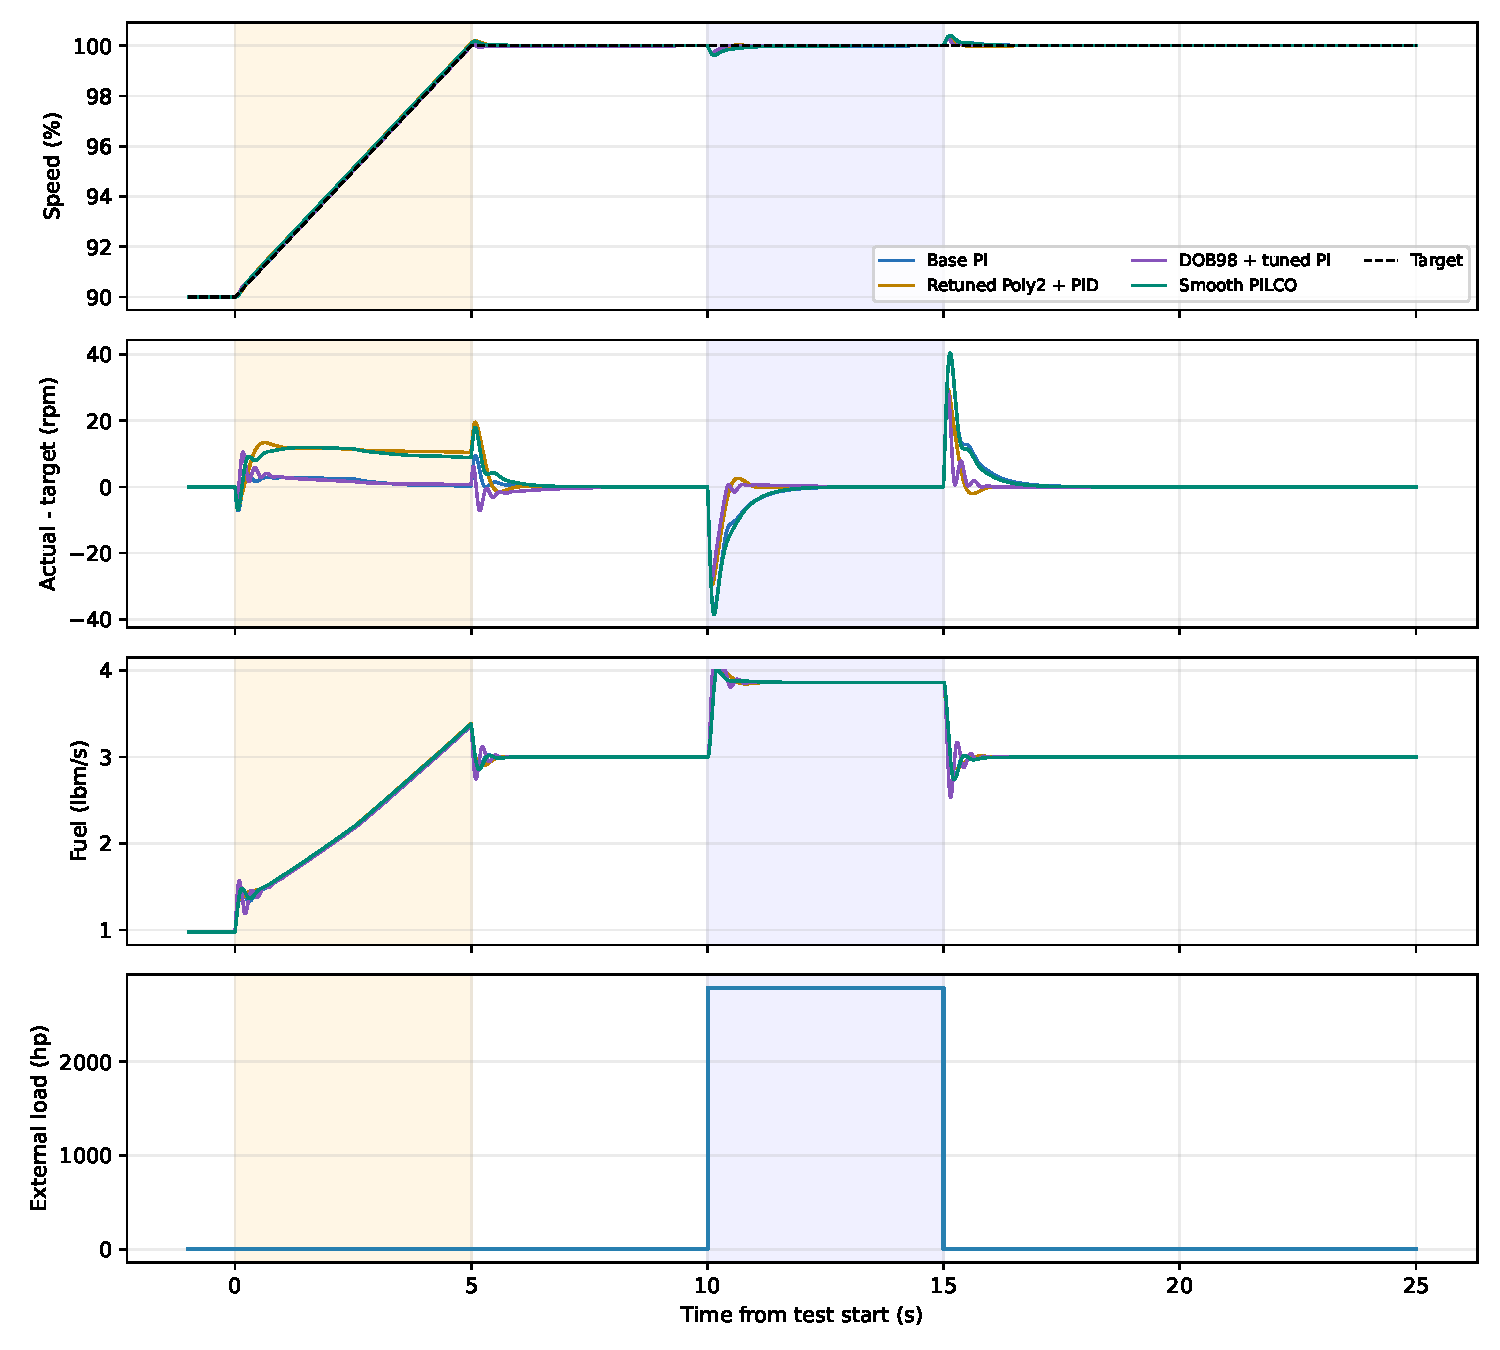
\includegraphics[width=\textwidth,height=.68\textheight,keepaspectratio]{late4_responses.pdf}
\subsection{Results and limits}
\begin{center}\small\begin{tabular}{lrrr}\toprule Controller & Ramp RMSE & Load/recovery RMSE & Full RMSE\\ & rpm & rpm & rpm\\\midrule
Base PI & 2.161 & 6.815 & 5.408 \\
Retuned Poly2 + PID & 10.949 & 4.416 & 6.214 \\
DOB98 + tuned PI & 2.459 & 3.710 & 3.142 \\
Smooth PILCO & 10.252 & 6.913 & 7.207 \\
\bottomrule\end{tabular}\end{center}
\begin{center}\small\begin{tabular}{lrrr}\toprule Controller & Load peak $|e|$ & Load excess TV & Min. surge\\ & rpm & lbm/s & \%\\\midrule
Base PI & 40.13 & 0.945 & 7.64 \\
Retuned Poly2 + PID & 29.39 & 0.696 & 7.75 \\
DOB98 + tuned PI & 29.10 & 2.184 & 7.74 \\
Smooth PILCO & 40.47 & 0.919 & 7.63 \\
\bottomrule\end{tabular}\end{center}
Errors use actual shaft speed, not sensed speed. Ramp RMSE covers 0--5 s; load/recovery RMSE covers 10--25.005 s; full RMSE covers the entire cycle. Load excess TV sums the 10--15 and 15--25.005 s segments. Sample interval is 0.015 s; first logged load-on is 10.005 s, and load-off is 15.000 s.

\textbf{Contribution of each change.} Base PI full-cycle RMSE is 5.408 rpm. Adding the DOB while retaining the original PI gains gives 4.546 rpm. Retuning PI with the DOB enabled gives 3.142 rpm. This ablation separates observer addition from gain tuning.

\textbf{Independent scenario check.} The selected gains are frozen and tested on a four-second speed ramp with a 5\% load pulse at seconds 10--15. Full-cycle RMSE is 2.024 rpm; minimum surge margin is 11.14\%. This check does not enter selection and is not a comparison against retuned baselines on that second scenario.

The requested combined cycle is a tuning case for DOB+PI, while the other gains were frozen from earlier studies. Consequently this is a comparison of the resulting controllers, not an equal-budget optimization contest. A local nominal model plus a DOB can tolerate some mismatch, but the small-excitation fit alone does not prove accuracy over 9000--10000 rpm. These nominal simulations are not a robust-stability proof. Fuel limits and compensation limits remain active parts of the implementation; the CSV records saturation and observer traces.
\subsection{Reproduction}
Run \path{dob98_identify_batch.m}, then \path{fit_dob98_model.py}, then \path{dob98_tune_batch.m}. The saved controller is \path{GasTurbine_DOB98_PI.mdl}, initialized by \path{tmats_dob98_setup.m}. Run \path{validate_dob98.py} for independent replay checks and \path{build_dob98_deliverables.py} for the revised figures and video. Data and selected parameters are under \path{results/dob98_pi_20261010}. Existing T-MATS workspace dependencies are required.


\section{Detailed interpretation of the final sensor and DOB results}
\subsection{Actual and sensed tracking answer different questions}
The sensor audit gives a particularly clear matched comparison because every maximum difference between the old and explicitly equalized trace is zero for actual speed, sensed speed, and fuel. The audit therefore rules out different sensor settings as the reason for the observed ordering. It does not imply that actual and sensed tracking errors are interchangeable.
\begin{table}[htbp]\centering\small
\begin{tabular}{lrr}\toprule Controller & Actual-speed ramp RMSE & Sensed-speed ramp RMSE\\ & rpm & rpm\\\midrule
Base PI & 2.160858 & 10.051133\\
Retuned Poly2 + PID & 10.948833 & 3.198864\\
Original PILCO-style PI & 11.223721 & 1.547154\\
Smooth PILCO & 10.251905 & 3.081877\\\bottomrule
\end{tabular}\caption{The same ramp scored using different signals. Values are from the archived sensor-comparison CSV; no new simulation is involved.}\end{table}
The original PILCO policy is closest to the target in sensed-speed RMSE and farthest in actual-speed RMSE among these four. A reader examining only the feedback error could therefore reach a different conclusion from the primary actual-speed comparison. For physical shaft regulation, the actual quantity is the relevant evaluation signal in this ideal simulation. In hardware it would need an independently justified measurement or state estimate.

\subsection{Deriving the local 9800-rpm identification explicitly}
Define $y_k=N_k-N_0$ and $v_k=u_k-u_0$. For each accepted identification transition, the equation $y_{k+1}=ay_k+bv_k+\epsilon_k$ supplies one row of the regression matrix:
\begin{equation}
\underbrace{\begin{bmatrix}y_1\\y_2\\\vdots\\y_M\end{bmatrix}}_{Y}
=\underbrace{\begin{bmatrix}y_0&v_0\\y_1&v_1\\\vdots&\vdots\\y_{M-1}&v_{M-1}\end{bmatrix}}_{X}
\underbrace{\begin{bmatrix}a\\b\end{bmatrix}}_{\theta}+\epsilon.
\end{equation}
Least squares chooses $\hat\theta$ to minimize $\|Y-X\theta\|^2$. The formula $(X^\top X)^{-1}X^\top Y$ explains the solution when full rank holds; numerically, a linear least-squares solver avoids unnecessary explicit inversion. The input must be the applied fuel including the excitation, because identifying against the injected perturbation alone would omit the stabilizing PI action.

One-step prediction uses the true $y_k$ in each row. Free-run prediction starts from an initial value and recursively uses $\hat y_k$. The archived model reports training one-step RMSE $1.7911\times10^{-4}$ rpm and free-run RMSE 0.003258 rpm. On the separate multisine record these are $9.8925\times10^{-5}$ and 0.001406 rpm. The small errors describe a speed range of only 9796.735--9803.056 rpm. A tiny local prediction error is entirely compatible with substantial mismatch at 9000 rpm or under a large external load.

\subsection{A directly implementable filtered inverse}
Write $r_f=e^{-2\pi f_cT_s}$ for the filter pole, to avoid confusing it with the speed reference, and define
\begin{equation}c_f=\frac{(1-r_f)^2}{b(1-p)},\quad
F(q)=\frac{Q}{P_nH}=c_f\frac{1-(a+p)q+apq^2}{1-2r_fq+r_f^2q^2}.
\end{equation}
If $w_k=N_{s,k}-N_0$ and $z=Fw$, then
\begin{equation}z_k=2r_fz_{k-1}-r_f^2z_{k-2}+c_f[w_k-(a+p)w_{k-1}+apw_{k-2}].
\end{equation}
The parallel filtered-command branch $h=Qv$ follows
\begin{equation}h_k=2r_fh_{k-1}-r_f^2h_{k-2}+(1-r_f)^2v_{k-2}.
\end{equation}
Thus the raw estimate is $z_k-h_k$. These recurrences explain why the two nominal delays are necessary in $Q$: the speed-inverse branch can be calculated from current and previous measurements, while the command branch explicitly retains the two delays. The construction uses the known saturated command; it does not read the external load schedule. Its poles are the filter poles, inside the unit circle, after the analytical cancellation specified by the model.

The trim latch subtracts the settled bias at handover. It removes a constant initial mismatch; it does not adapt the nominal model as speed changes. The compensation gain 0.7 and bound of 1 lbm/s are fixed during the PI search. The recorded maximum compensation in the selected main run is about 0.428413 lbm/s, below this compensation bound. The fuel command can nevertheless saturate because its total includes PI action as well as observer correction.

\subsection{What PI retuning bought and what it cost}
Adding the observer with the original gains reduces full-cycle RMSE from 5.407708 to 4.546279 rpm. Retuning to $(K_p,K_i)=(0.048,0.05)$ reduces it further to 3.142353 rpm. However, the original-gain DOB has ramp RMSE 1.441616 rpm, compared with 2.458988 rpm after retuning. The selected policy therefore trades some ramp performance for improved load/recovery behavior under the declared full-cycle objective.

The objective adds $0.05R_{\rm seg}$ to full RMSE. Its excess-variation windows include both the ramp and load phases. The load-only excess TV in the comparison table is a different subtotal. For the selected candidate these values are 4.085550 and 2.184455 lbm/s respectively. Confusing them would make the objective appear inconsistent with the displayed comparison. The selected controller also spends 1.139\% of full-cycle samples at a fuel limit, compared with 0.659\% for base PI. Better tracking is accompanied by additional actuator activity.

\subsection{The complete saved PI search}
\begin{table}[htbp]\centering\small\begin{tabular}{rrrrrrr}\toprule Case & $K_p$ & $K_i$ & Full RMSE & Ramp RMSE & $R_{\rm seg}$ & Objective\\\midrule
1 & 0.025 & 0.050 & 4.5463 & 1.4416 & 1.6970 & 4.6311\\
2 & 0.015 & 0.025 & 7.3993 & 7.9607 & 0.9555 & 7.4470\\
3 & 0.015 & 0.050 & 6.6614 & 2.0759 & 1.6012 & 6.7414\\
4 & 0.015 & 0.100 & 7.2924 & 5.7493 & 3.8650 & 7.4857\\
5 & 0.025 & 0.025 & 5.5285 & 6.6983 & 1.3702 & 5.5970\\
6 & 0.025 & 0.100 & 5.2704 & 5.4682 & 2.7144 & 5.4061\\
7 & 0.040 & 0.025 & 4.5578 & 5.3052 & 2.7683 & 4.6962\\
8 & 0.040 & 0.050 & 3.3854 & 2.0343 & 3.0062 & 3.5357\\
9 & 0.040 & 0.100 & 4.1326 & 5.5323 & 3.7298 & 4.3191\\
10 & 0.032 & 0.050 & 3.8400 & 1.6350 & 2.1835 & 3.9492\\
11 & 0.048 & 0.050 & 3.1424 & 2.4590 & 4.0855 & 3.3466\\
12 & 0.040 & 0.040 & 3.4183 & 1.7692 & 2.8927 & 3.5630\\
13 & 0.040 & 0.060 & 3.5107 & 2.9731 & 3.1287 & 3.6672\\
\bottomrule\end{tabular}\caption{All archived DOB98 PI candidates. RMSE is rpm; $R_{\rm seg}$ is lbm/s. Candidate 11 is selected by the stated objective.}\end{table}
Every candidate in the saved table is numerically accepted. This table describes a finite nine-pair search plus four refinements. It is not a proof that no untested pair could improve the objective, nor an equal tuning-budget comparison with the frozen Poly2 and PILCO methods. Candidate 1 is particularly useful because it isolates adding the DOB while retaining the original PI gains.

\subsection{The independent scenario and replay checks}
The frozen selected controller is then evaluated with a four-second 9000--10000 rpm ramp, corresponding to 250 rpm/s, and a 5\% load pulse. Its full RMSE is 2.024232 rpm, ramp RMSE 3.289699 rpm, and load/recovery RMSE 1.702970 rpm; minimum recorded surge margin is 11.135\%. The ramp metric uses the four-second interval, not the five-second interval of the tuning case. Other controller families were not retuned and compared on this independent scenario, so this result supports transfer of the selected controller but not a new ranking.

Independent filter replay matches the recorded observer branch within approximately $2.4\times10^{-13}$ lbm/s. The nominal filtered-inverse identity has maximum numerical error around $6.5\times10^{-14}$. These checks support correct coefficient ordering, delay handling, and filter realization. They do not establish uncertainty calibration, noise robustness, or a global stability margin for the nonlinear plant. Their proper role is to remove implementation ambiguity before interpreting the accepted plant trajectories.



\chapter{Cross-study answers, attribution, and validity}
\label{ch:synthesis}
\section{RQ1: prediction quality is necessary for some uses, but not sufficient}
The identification studies distinguish three information patterns. An online one-step predictor is corrected by each newly observed output. A frozen free-running model must propagate its own past predictions. An inverse controller additionally needs suitable zeros, local sensitivity and signal timing. The same numerical fit cannot establish all three properties.

The ten-term RLS has a reported pre-update one-step fit of 99.8729 percent, but frozen held-out ramp fit is 62.6191 percent. The sparse model improves the held-out result to 65.2666 percent and lowers the reported regression conditioning problem, but it does not remove the gap between online prediction and free-running transfer. The raw acceleration model's near-unit nonminimum-phase zero also makes inversion a separate problem from prediction. The physical equilibrium correction and causal filter are therefore substantive design steps, not details justified by a high fit score.

For nominal GP regression, accurate output prediction again fails to guarantee good feedback. An inverse's derivative controls how a small speed or acceleration deviation changes command. Two models can give close predictions at sampled points while having different local slopes between them. In this archive, weak or negative slopes motivate normalization, guards and fallback. This establishes a control-design concern in the tested inverse, not a theorem that GPs have poor derivatives.

The DOB98 local model supplies an especially clear scope example. Its independent free-run error is about 0.001406 rpm, but training speed covers only 9796.735--9803.056 rpm. A 9000--10000 rpm ramp spans a much larger region. The combined-cycle success is an observed closed-loop result; the local fit cannot be converted into a global model-error bound.

\section{RQ2: what the existing ablations identify}
\subsection{Constant feedforward and integral state}
At fixed reference and ambient conditions, let $c$ be a constant feedforward value. Compare $u_A=K_pe+I_A$ with $u_B=c+K_pe+I_B$. If $I_B(0)=I_A(0)-c$ and both integrators follow the same update, then $u_A=u_B$ for every sample for which the same conditional-integration decisions apply. Equal commands imply equal plant responses, preserving the equality inductively under matched implementations.

This is a coordinate shift in controller memory, not extra disturbance information. It explains the same-gain FF ablations. When feedforward becomes time varying, the shifted integral would require an additional compensating update, and the equivalence no longer follows automatically. The covered-cycle FF result must therefore be considered separately from fixed-reference load rejection.

\subsection{Inverse coordinates and equivalent PID action}
Locally, an inverse difference behaves approximately as $g_N e-g_a\hat a$ at a constant reference. PI action on that difference creates proportional, integral and acceleration-sensitive terms. Under the stated linearization, the effective coefficients include
\begin{equation}
K_{p,\mathrm{eff}}=K_p g_N+K_i g_a,\quad
K_{i,\mathrm{eff}}=K_i g_N,\quad
K_{d,\mathrm{eff}}=K_p g_a.
\end{equation}
The exact deployed realization also contains filtering, delay, saturation and possibly derivative variation, so these coefficients are a local explanation. They show why changing inverse slopes changes feedback behavior even if nominal fuel prediction remains accurate.

At the R3 target, RMSE is 1.75198 rpm and ringing is 1.45899; the matched filtered PID gives 1.74912 rpm and 1.42916. The correct conclusion is that no additional GP-specific advantage is demonstrated at that target. The environmental transfer record remains useful, but it does not erase this attribution result. A GP controller can perform well without its nonlinear representation being the cause of the local improvement.

\subsection{Changing representation before retuning}
On the covered cycle, the polynomial replacement gives full RMSE of about 0.676972 rpm compared with 0.702711 rpm for the GP version under the retained architecture. Base PI remains lower at about 0.591513 rpm. The polynomial's poorer regression score therefore does not prevent a competitive controller configuration. This is evidence against using nominal prediction error alone as a controller-selection criterion. It is not proof of a universal polynomial advantage or a statistical population difference.

The later 9250-rpm retune is a different comparison because gains change and the target is slightly below the old nominal training-speed range. Its lower local RMSE and ringing must be read alongside its larger peak error relative to original Poly2 and higher peak fuel slew than base PI. The fixed-gain substitution and the later tuning result should not be merged into one isolated ``model simplification benefit.''

\subsection{Observer addition and PI retuning}
The final combined-cycle results permit the following sequential comparison:
\begin{center}
\begin{tabular}{lrr}\toprule Configuration & Full RMSE (rpm) & Ramp RMSE (rpm)\\\midrule
Inherited PI & 5.407708 & 2.160858\\
DOB98 with original PI & 4.546279 & 1.441616\\
DOB98 with selected PI & 3.142353 & 2.458988\\\bottomrule
\end{tabular}
\end{center}
The first change is a reduction of about 15.9 percent in full RMSE; the next is about 30.9 percent relative to the original-gain DOB result. The final reduction relative to inherited PI is about 41.9 percent. These percentages have different denominators and must not be added. They describe the recorded path through configurations, not independent causal shares that would remain unchanged under another gain choice.

An equally tuned PI without DOB is missing. Consequently, the evidence does not answer whether a comparable conventional gain search could achieve the same full-cycle result. The observer improves the inherited-gain branch, and tuning improves the observer branch, but the interaction between architecture and tuning is not fully identified.

\section{RQ3: objective choice and sensing change the result}
\subsection{Repairing a policy is not baseline dominance}
On the 10 percent pulse case, original PILCO-style PI has RMSE about 1.19728 rpm and ringing 14.82523. The smooth version has RMSE 2.38773 rpm and ringing 2.08375. This is a large reduction in reversal, about 85.9 percent, purchased with worse tracking than the aggressive policy. Base PI ringing is approximately 2.07023. The smooth version therefore repairs the original policy's excessive reversal without establishing dominance over the conventional baseline.

The selected smooth gains, approximately 0.02480 and 0.05386, are close to the inherited PI values 0.025 and 0.05. This is consistent with the regularizer favoring a less aggressive controller. It does not prove that the probabilistic optimizer was unnecessary, because an equally budgeted direct search was not compared. It does limit a claim that the final behavior demonstrates an intrinsically superior learned control law.

The expectation calculation is exact for an absolute value of a Gaussian scalar with the supplied moments. The propagated trajectory distribution is an approximation, and the deployed controller includes saturation absent from the affine planning policy. ``Analytic expected penalty'' must therefore not be interpreted as exact expected fuel behavior of the nonlinear plant.

\subsection{Actual speed versus feedback measurement}
The no-load ramp is 200 rpm/s. A first-order sensor with time constant 0.05 s has a continuous steady-ramp lag of approximately 10 rpm; discrete timing contributes to the observed signal difference. A controller that keeps the lagged measurement close to the moving target may place actual speed ahead of it. Thus low sensed-error RMSE does not automatically mean low actual-error RMSE.

The archived actual/sensed ramp RMSE pairs are 2.160858/10.051133 rpm for base PI and 11.223721/1.547154 rpm for original PILCO-style PI. They order those controllers in opposite ways. The explicit equal-sensor rerun produces zero maximum trace differences for actual speed, sensed speed and fuel, so unequal sensor settings are ruled out as the explanation for the previous ordering.

The hypothesis that the base controller's response partly offsets sensor lag is consistent with this evidence. A zero-lag or compensated-sensor ablation was not performed. The causal role of that cancellation therefore remains an interpretation, not a completed isolated experiment. Version 2 makes this distinction explicit.

\subsection{No single actuator metric tells the whole story}
The final DOB's load-phase excess variation is 2.184455 compared with base PI's 0.944543, approximately a 131 percent increase. Its full segmented value is 4.085550, a different quantity used in the selection objective. Fuel-limit occupancy also increases from 0.659 to 1.139 percent. Lower full-cycle speed RMSE is therefore not evidence of uniformly smoother or less demanding actuation.

These numbers do not establish actuator damage. No actuator model or endurance experiment connects this metric directly to wear. They establish increased command activity under the stated definition and motivate reporting multiple constraints before declaring a practical winner.

\section{RQ4: transfer is limited and multidimensional}
The environmental grid, reduced-amplitude pulses and later ramps are useful precisely because they differ from local development cases. However, the broad cycle exhibits extensive out-of-domain and fallback exposure. The subsequently covered cycle is an informative revised scenario, not a test selected before the broad-cycle outcome was known. Its better coverage does not imply that the final 9250-rpm gains or the later DOB98 inherit validation over the entire grid.

The final DOB frozen-gain four-second ramp/5 percent pulse check supplies a second scenario. Because the complete comparator lineup was not evaluated there, it supports successful transfer of that controller configuration rather than superior transfer relative to all alternatives. The local predictor's independent multisine is also a different validation target: it tests local model prediction, not the controller's wide-range ranking.

No result in this archive tests sensor bias, noisy differentiation, uncertain component maps or a new engine family in a controlled campaign. The correct answer to RQ4 is therefore a map of demonstrated local transfers and known limits, not a single yes/no claim of robustness.

\section{Threats to validity and the remaining effect on claims}
\begin{longtable}{@{}p{.23\linewidth}p{.34\linewidth}p{.35\linewidth}@{}}
\toprule Threat & Existing mitigation & Remaining consequence\\\midrule\endhead
Unequal tuning opportunity & Original-gain DOB, unchanged-gain model substitution and matched PID retained & No general architectural superiority claim.\\
Selection on reported scenario & Explicit evidence-role ledger; held-out amplitude records distinguished & Main selection scores remain optimistic for generalization.\\
Narrow model support & Speed ranges, ambient coverage and fallback recorded & No global error or stability guarantee.\\
Measurement/metric ambiguity & Actual/sensed audit; common time step and local windows & Sensor-cancellation mechanism not isolated by a new ablation.\\
Numerical invalidity & Residual/iteration checks; rejected cases preserved & Validity conditional on solver and model conventions.\\
Statistical dependence & No pseudo-replicate confidence intervals or significance claims & Small numerical differences are descriptive.\\
Missing physical uncertainty & Explicit exclusion of noise, actuator and deterioration robustness claims & Nominal simulation cannot qualify hardware performance.\\
AI-assisted authorship and review & Disclosure, source preservation, defence questions & Independent mastery and acceptance require human examination.\\\bottomrule
\end{longtable}


\chapter{Conclusions, practical interpretation, and future work}
\label{ch:conclusions}
\section{Answer to the primary question}
Identified and learned models improve some tested configurations, but their benefit is conditional on how the model is used, which gains are selected, which scenario is applied and which signal is scored. The archive does not support one controller ranking across all tasks. It also does not support attributing every improvement over inherited PI to a learned representation.

The most discriminating existing evidence points to feedback architecture and tuning as major explanations. Constant-reference feedforward can be absorbed into an integral offset. A matched filtered PID reproduces the R3 target behavior. A polynomial inverse remains competitive despite worse nominal prediction. The final DOB improves the inherited-gain configuration, while its subsequent PI search further improves the full score and worsens some other metrics. These observations support a comparative engineering conclusion, not a claim that learning or observer methods are universally ineffective.

\section{Conclusions organized by contribution}
\textbf{C1: Evidence discipline.} The revised ledger makes the data's role explicit for each model and controller. Numerically accepted trajectories, model coverage, parameter selection, frozen transfer and algebraic checks are treated separately. Failed runs remain visible. This enables a reader to determine what a result can support before interpreting its size.

\textbf{C2: Attribution.} Existing substitutions and ablations support several local mechanisms and expose missing comparisons. The thesis can explain why some apparent feedforward or GP benefits are not independently attributable to those elements. It cannot quantify an architecture-only improvement over an equally tuned PI for the final DOB case.

\textbf{C3: Performance tradeoffs.} Lower tracking error can accompany greater reversal, larger peak error, higher slew or more saturation. The no-load ramp also demonstrates that actual and sensed tracking are different objectives. A controller must therefore be assessed against a stated application requirement, not a single favorable metric selected after seeing the result.

\textbf{C4: Technical adaptation.} The Gaussian expected excess-variation calculation provides a reproducible way to include a particular reversal objective in the restricted offline policy search. It substantially reduces reversal relative to the aggressive original policy. Its novelty and superiority over simpler smoothness objectives are not established, and zero excess variation is not a bound on slew.

\section{Implications for choosing among the existing configurations}
For the recorded five-second no-load ramp scored on actual speed, inherited PI has the lowest error among the tested frozen policies. For the 9250-rpm load experiments, retuned Poly2 offers a useful local tracking/reversal tradeoff. Original PILCO-style PI emphasizes tracking at a large reversal cost; the smooth version moves toward the baseline tradeoff. For the final combined cycle used in its tuning, DOB98 plus selected PI has the lowest full-cycle RMSE of the revised lineup, with higher command activity than base PI.

These statements identify suitable starting points for further engineering evaluation. They are not deployment recommendations for a real engine. If an application imposes a hard slew, peak-speed, actuator or protection constraint, the preferred configuration may change. The archive lacks a quantified real-world requirement against which to make that decision.

\section{A future protocol for the unresolved architecture question}
The first new study should answer the missing comparison, rather than introduce another controller name. Choose a common plant/sensor/actuator setup and a declared training set of ramp and load scenarios. Compare PI, filtered PID, DOB plus PI and the selected inverse architecture with comparable gain-search budgets. Define the objective, bounds, numerical acceptance and operating-domain criteria before examining test results. Tune each architecture on the training scenarios only.

Next, freeze every controller and evaluate a separate set of speeds, ramp rates, pulse amplitudes and ambient conditions. Include the same reference and applied load for every comparator and report both full and phase-specific errors. Save the true and sensed outputs, requested and applied fuel, controller states, clipping and convergence flags. Retain failed cases in the reported acceptance rate.

To isolate components, include observer off/on at matched gains and PI-only/DOB-plus-PI after separate equal-budget tuning. This creates the missing comparison between the effect of adding an observer and the best result achievable by tuning within each family. It does not require claiming that one gain pair is universally optimal.

These are proposed experiments. They were not performed for this version, and the present conclusions do not depend on pretending that they were.

\section{A future protocol for the penalty and robustness questions}
For the ringing objective, compare excess variation, ordinary total variation and squared command increments using the same policy class, dynamics data, optimizer budget and constraints. Preserve peak slew and saturation as separate measurements. Test whether an event-window penalty merely moves aggression outside the scored window. If uncertainty propagation is claimed to improve policy selection, compare it with a matched mean-dynamics planning procedure.

For robustness, introduce measurement noise, bias, actuator lag and plant perturbations separately before combining them. The disturbance observer's filter must be evaluated against the resulting noise-versus-rejection tradeoff. A local-model schedule or richer nominal model can then be compared with the single 9800-rpm model. Any stability analysis should state its model, uncertainty class, switching assumptions and saturation treatment explicitly.

Hardware or hardware-in-the-loop work would address additional implementation and physical questions. It is not automatically required to make the present descriptive findings valid; it is required before treating those findings as qualification of a physical installation. None of these future tasks is counted as a completed contribution here.

\section{Master's revision status}
Version 2 addresses the jury's documentary concerns by specifying one primary question, distinguishing established methods from contributions, classifying evidence roles, foregrounding ablations, and limiting claims. The detailed technical account is preserved in a thematic structure rather than presented as an automatic progression toward a superior controller.

The missing equal-budget experiments and physical robustness evidence remain limitations. Because universal superiority and robustness are no longer claimed, their absence does not contradict the revised scope. An actual master's examination must still evaluate the candidate's independent understanding, ownership of the work and compliance with institutional requirements. This document is a revised submission candidate, not a self-issued acceptance certificate.

\appendix
\chapter{Response to the jury-style examination}
\label{app:jury}
\section{Purpose and status conventions}
The response addresses the written assessment dated 11 October 2026~\cite{jury}. ``Addressed in the manuscript'' means the framing, explanation or reporting has been changed. ``Claim narrowed'' means missing evidence is explicitly acknowledged and the stronger claim is not made. ``Requires examination'' means the issue cannot be resolved by writing a report. No status implies an institutional degree decision.

\small
\begin{longtable}{@{}p{.18\linewidth}p{.37\linewidth}p{.17\linewidth}p{.19\linewidth}@{}}
\toprule Jury issue & Revision and evidence & Status & Location\\\midrule\endhead
Unfocused research question & One primary question with four answerable subsidiary questions; contributions C1--C4 bounded to the archive & Addressed in manuscript & Chs.~\ref{ch:question}, \ref{ch:synthesis}\\
Literature gap and novelty unclear & Targeted primary-source comparison; established methods separated from application findings and unestablished penalty originality & Addressed; no first-in-literature claim & Ch.~\ref{ch:literature}\\
Unequal baseline tuning & Missing equally retuned PI explicitly stated; final result described as configured-system improvement & Claim narrowed; comparison not performed & Chs.~\ref{ch:protocol}, \ref{ch:synthesis}\\
Selection and validation mixed & Study-by-study ledger distinguishes predictor fit, controller selection, frozen transfer and replay & Addressed in manuscript & Ch.~\ref{ch:protocol}\\
Strong local fit overinterpreted & DOB98 range 9796.735--9803.056 rpm stated alongside wider ramp; no global error bound & Claim narrowed & Chs.~\ref{ch:dob98}, \ref{ch:synthesis}\\
Verification confused with robustness & Algebra, GP moment checks, nominal trajectories and physical uncertainty assigned separate roles & Addressed; robustness untested & Chs.~\ref{ch:protocol}, \ref{ch:synthesis}\\
PILCO terminology too broad & Consistent description as offline two-gain PILCO-style adaptation; planning/deployment differences identified & Addressed in manuscript & Chs.~\ref{ch:literature}, \ref{ch:policy}\\
Ringing repair portrayed as superiority & Original/smooth/base comparison and monotonic-command limitation made explicit & Claim narrowed & Chs.~\ref{ch:policy}, \ref{ch:synthesis}\\
Matched PID and FF ablations underemphasized & Added central attribution argument; fixed-reference equivalence and local PID interpretation explained & Addressed in manuscript & Ch.~\ref{ch:synthesis}\\
Sensor explanation overstated & Equal-sensor replay separated from untested causal cancellation hypothesis; actual/sensed scoring shown & Claim narrowed & Chs.~\ref{ch:transfer}, \ref{ch:synthesis}\\
Archive breadth obscures argument & Technical material consolidated into thematic chapters; explicit cross-study answers precede final conclusions & Addressed in manuscript & Chs.~\ref{ch:question}--\ref{ch:conclusions}\\
Candidate's independent mastery & Authorship disclosure and defence questions preserved; no claim that text proves independence & Requires human examination & Front matter; this appendix\\\bottomrule
\end{longtable}
\normalsize

\section{Response to the six master's requirements}
\subsection{Focused question and contribution statement}
The revised question concerns attribution within the archived campaign. C1--C4 define the contributions without claiming that any standard component is newly invented. The abstract reports both favorable and limiting evidence. The conclusion answers the same question rather than presenting the last controller as the inevitable winner.

\subsection{Literature comparison}
The new literature chapter explains the relevance of orthogonal identification, established DOB methods, prior GP engine feedforward, original PILCO and smooth-action regularization. It identifies the expected excess-variation construction as an adaptation whose originality has not been established. External papers provide methodological context, not substitute data for this turbine. The review's targeted scope is disclosed.

\subsection{Training, selection and held-out evaluation}
The ledger records dataset roles for the complete experimental progression. In particular, the 10 percent smooth-policy case is a selection case even though part of the original transition record was withheld from GP fitting. The final combined cycle is selection evidence for DOB98 gains and transfer evidence for frozen comparators. The four-second/5 percent check is not called comparative superiority because the full comparator lineup is absent.

\subsection{Conclusions limited to the tested conditions}
Architectural dominance, global robustness, GP uncertainty as a physical error bound, and fuel-economy benefits are not claimed. The local model range and the actual/sensed speed distinction appear in the main argument. Rounding in synthesis tables is explicitly descriptive; full-precision archived results remain available.

\subsection{Central discussion of discriminating evidence}
The synthesis uses the matched-PID result, constant-FF equivalence, GP-to-polynomial substitution, sensor audit and original-gain DOB branch as its principal attribution evidence. It explains the missing comparisons as carefully as the successful ones. This changes the thesis from a catalogue of algorithms into an argument about what the experiments can identify.

\subsection{Independent defence}
The report can provide equations, records and questions, but cannot conduct an oral examination or certify the candidate's independent mastery. This requirement is left open. The candidate should be able to reconstruct the reasoning below and trace numerical claims to the source rather than merely repeat the revised conclusion.

\section{Defence questions and the reasoning an answer should contain}
\textbf{Why can matched PID reproduce R3 locally?} An adequate answer should linearize the inverse map, identify how its derivatives scale static and acceleration terms, and explain the effect of normalization. It should also state why local equivalence does not imply global identity under changing derivatives, fallback or saturation.

\textbf{What uncertainty does the GP represent?} The answer should distinguish posterior uncertainty conditional on nominal data and a kernel from unknown shaft-load mismatch, sensor bias and physical parameter variation. It should explain why low posterior variance cannot alone choose a safe gain direction.

\textbf{What does the DOB ablation identify?} The answer should state the original-gain improvement and the subsequent tuning improvement, then identify the missing tuned-PI-only branch. It should not add percentage reductions with different denominators or interpret sequential differences as architecture-independent causal shares.

\textbf{Can zero ringing conceal an aggressive command?} The answer should give a monotone step as a counterexample, derive zero excess variation from equality between total variation and net change, and distinguish that result from peak slew or fuel mass.

\textbf{Why is the inverse causal?} The answer should account for the delays in the nominal plant and sensor, the two delays included in the Q filter, and the resulting implementable recurrence. It should distinguish stability of that filtered nominal inverse from robust stability of the complete nonlinear loop.

\textbf{Why do actual and sensed rankings differ?} The answer should derive the approximate ramp lag, identify which signal enters feedback and which is scored, and state that identical sensor settings do not imply identical responses to the lag.

\textbf{What contribution remains after prior art is acknowledged?} The answer should identify the comparative findings and their application-specific limits, rather than asserting invention of GP, PI, DOB or smooth-action costs. It should state the limited novelty status of the event-window adaptation.

\section{Preservation and reproducibility of this revision}
Version 1 remains unchanged. The V2 build assembles the archived derivations and figures with new framing, a literature chapter, an evidence ledger, a synthesis and this response. The source bundle retains the original evidence manifest and adds a revision manifest. Compilation and PDF checks do not invoke MATLAB, fit a model or tune a controller. Rebuilding the document is therefore distinct from rerunning the experiments.

The directory register describes the full workspace history, not the contents of this portable document package. The repository study map and companion archive identify the raw experiments and simulation dependencies.


\chapter{Complete early and fixed-controller result tables}
\label{app:early}
The following tables preserve rejected full trajectories as dashes. They are not imputed as zero, assigned a finite failure penalty, or silently omitted from acceptance counts. R and S denote ramped and stepped \emph{shaft load}; the reference is constant during evaluation. These tables should not be pooled with the later moving-speed-cycle reversal metric.
\begin{table}[htbp]\centering\small\setlength{\tabcolsep}{4pt}\begin{tabular}{@{}lrrrr@{}}\toprule
rpm/\%/type & Initial & FF retune & SD down & SD up\\\midrule
9000/5/R & 0.3706 & 0.2512 & 0.3378 & 0.2501\\
9000/10/R & 0.7441 & 0.5045 & 0.6797 & 0.5021\\
9000/20/R & 1.581 & 1.072 & 1.452 & 1.066\\
9000/30/R & 2.467 & 1.671 & 2.284 & 1.659\\
9500/5/R & 0.5222 & 0.3547 & 0.4601 & 0.3546\\
9500/10/R & 1.091 & 0.7414 & 0.9616 & 0.7413\\
9500/20/R & 2.284 & 1.552 & 2.012 & 1.552\\
9500/30/R & 3.681 & -- & -- & --\\
9500/20/S & 3.095 & -- & 3.758 & --\\
9500/30/S & -- & -- & -- & --\\
\bottomrule\end{tabular}\caption{All early scenarios: speed RMSE (rpm). R: ramped load; S: stepped load. A dash is a rejected full trajectory, not zero (D02).}\label{tab:early_rmse}\end{table}
\begin{table}[htbp]\centering\small\setlength{\tabcolsep}{4pt}\begin{tabular}{@{}lrrrr@{}}\toprule
rpm/\%/type & Initial & FF retune & SD down & SD up\\\midrule
9000/5/R & 0.369 & 0.6762 & 0.2579 & 0.6901\\
9000/10/R & 0.7169 & 1.328 & 0.5075 & 1.356\\
9000/20/R & 1.09 & 2.601 & 0.9559 & 2.666\\
9000/30/R & 1.345 & 3.329 & 1.243 & 3.419\\
9500/5/R & 0.5508 & 0.8865 & 0.442 & 0.8868\\
9500/10/R & 0.9796 & 1.961 & 0.892 & 1.962\\
9500/20/R & 1.629 & 4.128 & 1.74 & 4.13\\
9500/30/R & 1.958 & -- & -- & --\\
9500/20/S & 61.84 & -- & 13.34 & --\\
9500/30/S & -- & -- & -- & --\\
\bottomrule\end{tabular}\caption{All early scenarios: load-edge fuel ringing (lbm/s). R: ramped load; S: stepped load. A dash is a rejected full trajectory, not zero (D02).}\label{tab:early_ring}\end{table}
\clearpage
\section{Four fixed controllers}
\label{app:fixed}
The inverse-controller gains are 2/30 in all four-way comparisons. Their near-equal no-direct-FF and direct-FF scores provide the repeated constant-reference equivalence check. Base PI and base PI + FF retain the inherited 0.025/0.05 gains.
\begin{table}[htbp]\centering\small\setlength{\tabcolsep}{4pt}\begin{tabular}{@{}lrrrr@{}}\toprule
rpm/\%/type & P & PF & V & VF\\\midrule
9000/5/R & 0.5942 & 0.6014 & 0.499 & 0.499\\
9000/10/R & 1.193 & 1.208 & 1.002 & 1.002\\
9000/20/R & 2.54 & 2.571 & 2.131 & 2.131\\
9000/30/R & 3.973 & 4.022 & 3.327 & 3.327\\
9500/5/R & 1.017 & 1.049 & 0.7035 & 0.7035\\
9500/10/R & 2.125 & 2.192 & 1.47 & 1.47\\
9500/20/R & 4.453 & 4.593 & 3.078 & 3.078\\
9500/30/R & -- & -- & -- & --\\
9500/20/S & 6.43 & 6.712 & 4.054 & 4.054\\
9500/30/S & -- & -- & -- & --\\
9500/5/S & 1.484 & 1.548 & 0.9304 & 0.9304\\
\bottomrule\end{tabular}\caption{Four fixed controllers: speed RMSE (rpm). P: base PI; PF: base PI + FF; V: inverse PI; VF: inverse PI + FF (D04).}\label{tab:fixed_rmse}\end{table}
\begin{table}[htbp]\centering\small\setlength{\tabcolsep}{4pt}\begin{tabular}{@{}lrrrr@{}}\toprule
rpm/\%/type & P & PF & V & VF\\\midrule
9000/5/R & 0.138 & 0.1397 & 0.1007 & 0.1007\\
9000/10/R & 0.2756 & 0.2791 & 0.2003 & 0.2003\\
9000/20/R & 0.5898 & 0.5987 & 0.3934 & 0.3934\\
9000/30/R & 0.9456 & 0.9571 & 0.5517 & 0.5517\\
9500/5/R & 0.1977 & 0.2056 & 0.1575 & 0.1575\\
9500/10/R & 0.417 & 0.4339 & 0.3186 & 0.3186\\
9500/20/R & 0.8916 & 0.9262 & 0.629 & 0.629\\
9500/30/R & -- & -- & -- & --\\
9500/20/S & 4.705 & 4.315 & 9.169 & 9.169\\
9500/30/S & -- & -- & -- & --\\
9500/5/S & 1.195 & 1.089 & 2.488 & 2.488\\
\bottomrule\end{tabular}\caption{Four fixed controllers: fuel ringing (lbm/s). P: base PI; PF: base PI + FF; V: inverse PI; VF: inverse PI + FF (D04).}\label{tab:fixed_ring}\end{table}
\begin{table}[htbp]\centering\small\setlength{\tabcolsep}{4pt}\begin{tabular}{@{}lrrrr@{}}\toprule
rpm/\%/type & P & PF & V & VF\\\midrule
9000/5/R & 4.095 & 4.08 & 5.055 & 5.055\\
9000/10/R & 4.44 & 4.395 & 5.67 & 5.67\\
9000/20/R & 4.77 & 4.755 & 6.33 & 6.33\\
9000/30/R & 4.965 & 4.935 & 6.705 & 6.705\\
9500/5/R & 4.38 & 4.26 & 5.1 & 5.1\\
9500/10/R & 4.725 & 4.56 & 5.7 & 5.7\\
9500/20/R & 5.055 & 4.875 & 6.285 & 6.285\\
9500/30/R & -- & -- & -- & --\\
9500/20/S & 2.985 & 2.745 & 4.335 & 4.335\\
9500/30/S & -- & -- & -- & --\\
9500/5/S & 2.265 & 2.1 & 3.165 & 3.165\\
\bottomrule\end{tabular}\caption{Four fixed controllers: persistent recovery to 0.1 rpm (s). P: base PI; PF: base PI + FF; V: inverse PI; VF: inverse PI + FF (D04).}\label{tab:fixed_fine}\end{table}
\clearpage

\chapter{Environmental transfer and inverse-slope audit}
\label{app:grid}
Table~\ref{tab:environment_all} gives the complete environmental grid. The reference speed is 9500 rpm, load is 10\% of the condition-specific unloaded reference, and R3 includes static FF. Ratios below one favor the challenger for that metric. Fallback percentages must be interpreted with the separate map-range discussion in the main text. A 35/35 paired improvement in this table is not a robustness theorem outside the simulated plant family.
{\small\setlength{\tabcolsep}{4pt}\begin{longtable}{@{}lrrrrrrrrr@{}}
\caption{Complete 35-condition transfer audit, 9500 rpm / 10\% load steps. The four middle ratios are speed RMSE relative to base PI. V: previous inverse PI; R3 includes static FF. A dash means rejected. FB: R3 fallback percentage (D07).}\label{tab:environment_all}\\\toprule $h$ & ISA & P RMSE & P ring & V/P & R1/P & R2/P & R3/P & R3 ring/P & FB\%\\\midrule
\endfirsthead\toprule $h$ & ISA & P RMSE & P ring & V/P & R1/P & R2/P & R3/P & R3 ring/P & FB\%\\\midrule
\endhead\bottomrule\endfoot
0 & +0 & 3.08 & 2.371 & 0.6304 & 0.8388 & 0.6832 & 0.6931 & 0.7633 & 0\\
2500 & +0 & 2.883 & 2.246 & 0.6772 & 0.9051 & 0.8088 & 0.692 & 0.724 & 0\\
5000 & +0 & 2.485 & 2.189 & 1.035 & 1.402 & 2.014 & 0.6888 & 0.6968 & 0\\
7500 & +0 & 1.874 & 1.705 & 1.128 & 1.528 & 2.483 & 0.6878 & 0.6884 & 0\\
10000 & +0 & 1.247 & 1.281 & 5.018 & 6.966 & -- & 0.6825 & 0.6972 & 100\\
0 & -10 & 3.529 & 2.554 & 0.5924 & 0.7858 & 0.6118 & 0.6942 & 0.7504 & 0\\
2500 & -10 & 3.223 & 2.461 & 0.6668 & 0.8921 & 0.7919 & 0.6967 & 0.7384 & 0\\
5000 & -10 & 2.576 & 2.283 & 1.018 & 1.377 & 1.92 & 0.688 & 0.6997 & 0\\
7500 & -10 & 1.86 & 1.869 & 16.72 & 22.1 & 73.57 & 0.6837 & 0.6788 & 100\\
10000 & -10 & 1.173 & 1.26 & 6.057 & 8.275 & -- & 0.6801 & 0.7319 & 100\\
0 & +10 & 2.72 & 2.17 & 0.6583 & 0.8777 & 0.7518 & 0.6911 & 0.7578 & 0\\
2500 & +10 & 2.517 & 1.998 & 0.6862 & 0.917 & 0.8203 & 0.6913 & 0.7324 & 0\\
5000 & +10 & 2.266 & 1.854 & 0.7719 & 1.037 & 1.069 & 0.6907 & 0.7109 & 0\\
7500 & +10 & 1.807 & 1.635 & 1.17 & 1.586 & 2.73 & 0.6873 & 0.686 & 0\\
10000 & +10 & 1.32 & 1.301 & 16.43 & 19.01 & -- & 0.6847 & 0.6706 & 100\\
0 & +20 & 2.354 & 1.934 & 0.6712 & 0.895 & 0.7815 & 0.6897 & 0.7757 & 0\\
2500 & +20 & 2.21 & 1.854 & 0.7472 & 1.002 & 0.9716 & 0.6898 & 0.7374 & 0\\
5000 & +20 & 2.008 & 1.656 & 0.7728 & 1.038 & 1.062 & 0.6905 & 0.711 & 0\\
7500 & +20 & 1.742 & 1.557 & 1.065 & 1.442 & 2.261 & 0.6898 & 0.6924 & 0\\
10000 & +20 & 1.289 & 1.192 & 1.318 & 1.789 & 3.861 & 0.6871 & 0.6815 & 0\\
0 & -20 & 4.007 & 2.866 & 0.5945 & 0.7893 & 0.6185 & 0.6946 & 0.7547 & 0\\
2500 & -20 & 3.457 & 2.956 & 0.8852 & 1.197 & 1.393 & 0.6913 & 0.7163 & 0\\
5000 & -20 & 2.705 & 2.553 & 1.461 & 2.011 & -- & 0.6224 & 0.9895 & 98.65\\
7500 & -20 & 1.756 & 1.84 & 8.034 & 10.94 & -- & 0.6815 & 0.7089 & 100\\
10000 & -20 & 1.111 & 1.251 & 6.17 & 8.438 & -- & 0.678 & 0.7532 & 100\\
0 & +30 & 2.003 & 1.73 & 0.6872 & 0.9162 & 0.7986 & 0.688 & 0.7981 & 0\\
2500 & +30 & 1.935 & 1.65 & 0.7522 & 1.008 & 0.9929 & 0.689 & 0.7424 & 0\\
5000 & +30 & 1.747 & 1.488 & 0.7927 & 1.065 & 1.105 & 0.6899 & 0.7227 & 0\\
7500 & +30 & 1.55 & 1.334 & 0.9076 & 1.225 & 1.514 & 0.6892 & 0.6924 & 0\\
10000 & +30 & 1.243 & 1.141 & 1.319 & 1.79 & 3.932 & 0.6872 & 0.6751 & 0\\
0 & -30 & 4.532 & 3.703 & 0.7908 & 1.061 & 1.064 & 0.6779 & 0.7823 & 0\\
2500 & -30 & 3.583 & 3.075 & 0.8843 & 1.194 & 1.383 & 0.6889 & 0.7107 & 0\\
5000 & -30 & 2.577 & 2.637 & 15.87 & 22.36 & 83.79 & 0.6828 & 0.6873 & 100\\
7500 & -30 & 1.649 & 1.809 & 13.46 & 18.31 & -- & 0.6788 & 0.7429 & 100\\
10000 & -30 & 1.052 & 1.251 & 4.714 & 6.386 & -- & 0.676 & 0.7828 & 100\\\end{longtable}}
The raw D08 derivative file contains all 36 target/grid operating-point diagnostics, including the nine locations with negative nominal static speed slope. It records both analytic-versus-numerical derivative checks and the corresponding ideal equivalent gains. Negative slopes are a feedback-coordinate concern even where the output fit is accurate; they are not automatically evidence of a wrong numerical derivative.

\chapter{Polynomial coefficients and full local gain search}
\label{app:poly}
The coefficient ordering is intercept, four linear terms, four squares, then six cross terms. Use the input means and scales stated in the full-quadratic-inverse chapter before evaluating the expression. Coefficients have fuel-flow units and are not gains. Full precision is retained in D14 and in the original JSON model; the printed table is rounded for readability.
\begin{table}[htbp]\centering\small\setlength{\tabcolsep}{4pt}\begin{tabular}{@{}lr@{}}\toprule
Term & Coefficient (lbm/s)\\\midrule
$1$ & 1.60113254059\\
$z_1$ & 0.119416371262\\
$z_2$ & 0.0540225588644\\
$z_3$ & -0.342237138763\\
$z_4$ & 0.711670738338\\
$z_1^2$ & -0.00361356608798\\
$z_2^2$ & 0.000977366025356\\
$z_3^2$ & -0.0800375317654\\
$z_4^2$ & 0.0232444919616\\
$z_1z_2$ & 0.00100931606766\\
$z_1z_3$ & 0.0366434140839\\
$z_1z_4$ & 0.0629030714395\\
$z_2z_3$ & 0.00136341822536\\
$z_2z_4$ & -0.000707278500721\\
$z_3z_4$ & -0.20459203567\\
\bottomrule\end{tabular}\caption{Full quadratic coefficients in standardized coordinates. All 15 terms are retained (D14).}\label{tab:polycoef}\end{table}
\clearpage
\section{All 9250 rpm tuning candidates}
The original gains form candidate 1. Candidates 2--28 are the coarse Cartesian grid; candidates 29--34 are the single coordinate-refinement round. All candidates use the same frozen model and pulse profile. Base PI is excluded from the objective and therefore omitted from this candidate table.
{\small\setlength{\tabcolsep}{4pt}\begin{longtable}{@{}lrrrrrr@{}}
\caption{All 34 tested Poly2 gain settings at 9250 rpm. All were numerically accepted; candidate 34 minimizes the stated joint score (D15).}\label{tab:tune_all}\\\toprule ID & $K_p$ & $K_i$ & $K_d$ & RMSE & Ringing & $J$\\\midrule
\endfirsthead\toprule ID & $K_p$ & $K_i$ & $K_d$ & RMSE & Ringing & $J$\\\midrule
\endhead\bottomrule\endfoot
1 & 0.025 & 0.1 & 0.002 & 1.6658 & 1.6968 & 1\\
2 & 0.015 & 0.08 & 0.001 & 2.47654 & 1.05239 & 1.48669\\
3 & 0.025 & 0.08 & 0.001 & 1.9035 & 0.940295 & 1.14269\\
4 & 0.035 & 0.08 & 0.001 & 1.61308 & 1.96343 & 1.15714\\
5 & 0.015 & 0.14 & 0.001 & 2.13254 & 2.30021 & 1.35562\\
6 & 0.025 & 0.14 & 0.001 & 1.58529 & 1.45065 & 0.951666\\
7 & 0.035 & 0.14 & 0.001 & 1.33132 & 2.19236 & 1.29206\\
8 & 0.015 & 0.2 & 0.001 & 2.07613 & 4.27141 & 2.51734\\
9 & 0.025 & 0.2 & 0.001 & 1.46863 & 2.19493 & 1.29357\\
10 & 0.035 & 0.2 & 0.001 & 1.21753 & 2.48137 & 1.46239\\
11 & 0.015 & 0.08 & 0.002 & 2.33302 & 1.26257 & 1.40054\\
12 & 0.025 & 0.08 & 0.002 & 1.82436 & 1.64788 & 1.09519\\
13 & 0.035 & 0.08 & 0.002 & 1.55644 & 2.72951 & 1.60862\\
14 & 0.015 & 0.14 & 0.002 & 1.90057 & 1.72301 & 1.14094\\
15 & 0.025 & 0.14 & 0.002 & 1.46746 & 1.84422 & 1.08688\\
16 & 0.035 & 0.14 & 0.002 & 1.24958 & 2.81321 & 1.65795\\
17 & 0.015 & 0.2 & 0.002 & 1.72149 & 2.34619 & 1.38272\\
18 & 0.025 & 0.2 & 0.002 & 1.30742 & 2.05752 & 1.21259\\
19 & 0.035 & 0.2 & 0.002 & 1.10962 & 2.90497 & 1.71203\\
20 & 0.015 & 0.08 & 0.003 & 2.25979 & 2.44295 & 1.43974\\
21 & 0.025 & 0.08 & 0.003 & 1.78329 & 3.22949 & 1.90329\\
22 & 0.035 & 0.08 & 0.003 & 1.5279 & 4.6707 & 2.75266\\
23 & 0.015 & 0.14 & 0.003 & 1.79248 & 2.71685 & 1.60116\\
24 & 0.025 & 0.14 & 0.003 & 1.40908 & 3.3398 & 1.9683\\
25 & 0.035 & 0.14 & 0.003 & 1.2097 & 4.72939 & 2.78725\\
26 & 0.015 & 0.2 & 0.003 & 1.5755 & 3.01185 & 1.77502\\
27 & 0.025 & 0.2 & 0.003 & 1.23212 & 3.44905 & 2.03268\\
28 & 0.035 & 0.2 & 0.003 & 1.05902 & 4.77544 & 2.81438\\
29 & 0.01875 & 0.14 & 0.001 & 1.86401 & 1.59225 & 1.11898\\
30 & 0.03125 & 0.14 & 0.001 & 1.40929 & 1.77466 & 1.04589\\
31 & 0.025 & 0.105 & 0.001 & 1.72922 & 1.09514 & 1.03807\\
32 & 0.025 & 0.175 & 0.001 & 1.50354 & 1.86286 & 1.09787\\
33 & 0.025 & 0.14 & 0.00075 & 1.63519 & 1.7329 & 1.02128\\
34 & 0.025 & 0.14 & 0.00125 & 1.54614 & 1.29904 & 0.928166\\\end{longtable}}

\chapter{Algorithm registry and reproducibility}
\label{app:repro}
\section{Controller identities}
\begin{longtable}{@{}p{.24\linewidth}p{.70\linewidth}@{}}
\toprule Name in this paper & Defining implementation distinction\\\midrule\endhead
Base PI & Direct sensed-speed error; fixed gains 0.025/0.05.\\
Base PI + FF & Early state-scheduled, equilibrium-subtracted, limited GP correction.\\
Initial inverse PI & Two inverse queries; dynamic fuel error in P and I; gains 4/40.\\
FF-retuned inverse & Direct setpoint inverse FF; residual integral; gains 3/60.\\
SD down / SD up & Same 3/60 base gains multiplied by the stated SD schedule; gain-change integral transfer.\\
Low-ringing inverse & Fixed gains 2/30 selected at 9500 rpm / 5\% steps.\\
Environmental inverse & Four-input exact GP; same 2/30 gains and direct static FF.\\
R1 & Dynamic virtual error retained; gains 1.5/22.\\
R2 & Static error integrated; attenuated acceleration fuel in proportional path; 16/40, $\beta=0.05$.\\
Historical R3 & Derivative normalization and guarded fallback, 0.025/0.1/0.002, including static FF.\\
R3-FB & Same R3 feedback but no direct static FF in command sum.\\
R3-GP & R3 plus $g(r,0,T,P)$; equals historical R3 on the covered cycle.\\
R3-P2 & Same R3 architecture and initial gains, replacing inverse values/derivatives by full quadratic regression.\\
Retuned Poly2 & R3-P2 with 0.025/0.14/0.00125 selected at 9250 rpm.\\
\bottomrule
\end{longtable}

\section{Primary evidence register}
The source archive includes the following numerical tables under \path{data/}, together with a JSON manifest containing the original relative path and SHA-256 hash. The local archive paths refer to the shared T-MATS workspace. Native MAT/CSV trajectories remain in the original study directories; the paper source archive contains the compact evidence tables and figures required to reproduce the manuscript, not the complete engine installation or every simulation trace.
{\footnotesize\begin{longtable}{@{}p{.07\linewidth}p{.90\linewidth}@{}}\toprule ID & Archived evidence file\\\midrule\endhead
\texttt{D01} & \path{results/inverse_gpr_20260913_150824_698/metrics.csv}\\
\texttt{D02} & \path{results/virtual_fuel_uqup_20260913_231743/comparison_all_methods.csv}\\
\texttt{D03} & \path{results/ff_lowgain_20260913_234549/tuning.csv}\\
\texttt{D04} & \path{results/four_fixed_20260913_235253/summary.csv}\\
\texttt{D05} & \path{results/environment_gpr_20260914_201325/gpr_metrics.csv}\\
\texttt{D06} & \path{results/environment_gpr_20260914_201325/comparison_summary.csv}\\
\texttt{D07} & \path{results/gpr_remedies_20260914_220633/remedy_comparison.csv}\\
\texttt{D08} & \path{results/gpr_remedies_20260914_220633/inverse_slope_diagnosis.csv}\\
\texttt{D09} & \path{results/gpr_remedies_20260914_220633/ablation_worker_01.csv}\\
\texttt{D10} & \path{results/r3_ambient_cycle_20260915/summary.csv}\\
\texttt{D11} & \path{results/r3_covered_cycle_20260915_final/coverage_summary.csv}\\
\texttt{D12} & \path{results/r3_poly2_challenger_20260915/summary.csv}\\
\texttt{D13} & \path{results/poly2_inverse_20260915/fit_metrics.csv}\\
\texttt{D14} & \path{results/poly2_inverse_20260915/coefficients.csv}\\
\texttt{D15} & \path{results/poly2_tune9250_20260915/tuning_scores.csv}\\
\texttt{D16} & \path{results/poly2_tune9250_20260915/validation_summary.csv}\\
\texttt{D17} & \path{results/poly2_tune9250_20260915/selected.csv}\\
\texttt{D18} & \path{results/environment_gpr_20260914_201325/test_200_points.csv}\\
\texttt{D19} & \path{results/r3_poly2_challenger_20260915/coverage_summary.csv}\\
\texttt{D20} & \path{results/poly2_tune9250_20260915/verification.csv}\\
\texttt{D21} & \path{results/virtual_fuel_ff_20260913_194955/same_gains_ablation.csv}\\
\texttt{D22} & \path{results/poly2_inverse_20260915/poly2_model.json}\\\bottomrule\end{longtable}}

\section{September-paper V2 review evidence}
The companion response records three separate AI role reviews and the author dispositions. The review files are preserved under \path{reviews/} in the source package. The supplementary \path{metric_sensitivity.csv} and its trace-hash manifest document the calculations in Section~\ref{sec:sensitivity}. The six supporting archived traces are included as \path{review_traces/}; they are unchanged simulator outputs, not additional experiments. The revision changes exposition and derived reporting only. The original paper and original numerical source tables remain preserved.

\section{Reproducing the historical September paper}
This subsection describes the September manuscript, not the present master\textquotesingle s revision. To typeset this report, compile \path{TMATS_Masters_Thesis_V2.tex} three times from the supplied V2 source directory. The older filenames below are preserved for historical reproducibility.

The assembled LaTeX source is \path{control_evolution_paper.tex}. The original tables are generated from archived CSV files by \path{build_control_evolution_paper.py}; V2 assembly is performed by \path{revise_control_evolution_paper.py}. The supplementary sensitivity tables are generated by \path{review_control_evolution_metrics.py}. New early scheduling figures are generated by \path{plot_control_evolution.m}; other figures are copied from the finalized stage-specific reports and hashed. Compile the assembled source at least twice with \path{pdflatex} to resolve chapter, table, figure, and bibliography references. No shell escape or network access is required for LaTeX compilation.

To reproduce simulations rather than typesetting, use the corresponding runners in the existing MATLAB/T-MATS workspace: \path{run_tmats_virtual_fuel_study.m}, \path{run_tmats_virtual_fuel_ff_study.m}, the UQ/UQUp runners, \path{run_tmats_four_fixed_comparison.m}, \path{run_tmats_environment_comparison.m}, \path{run_tmats_gpr_remedies.m}, \path{run_tmats_r3_cycle.m}, and \path{run_tmats_poly9250.m}. The study-specific setup files determine frozen model paths, load references, startup timing, and gains. Some runners resume existing results; use a new directory when a fresh numerical rerun is intended.

\section{Evidence exclusions and reader guidance}
The preliminary broad-cycle governor diagnostic, the 9400--9600 rpm hull-excursion attempt, and the superseded dynamic-acceleration FF attempt are historical diagnostics, not members of the final comparisons. Their exclusion is stated because they answer different implementation questions. Rejected plant trajectories in the final scenario banks remain represented in validity counts and as missing full-run scores.

The literature references support method definitions and intellectual context. They do not supply the numerical turbine performance claims, which come from D01--D22. The original doctoral work is cited for lineage only; its engine-airpath results are not transferred to this turbine. The paper makes no claim of external peer review, hardware validation, global optimization, or closed-loop robustness certification.

\clearpage

\chapter{Complete study-directory register}
The register covers every direct directory under the project results folder at assembly time. Counts are file counts, not independent simulations. Aggregate reports and repeated attempts are retained for provenance. A timestamp alone does not establish acceptance. The detailed reports and validity columns control interpretation.
\subsection*{\path|baseline_20260907_202021_071|}
Plant preparation, numerical acceptance, or identification input record. See the early experiment narrative for accepted and rejected variants. Archived file count: 4.
Entry files: \path|data.csv|, \path|metadata.json|.
\subsection*{\path|baseline_20260907_202114_161|}
Plant preparation, numerical acceptance, or identification input record. See the early experiment narrative for accepted and rejected variants. Archived file count: 4.
Entry files: \path|data.csv|, \path|metadata.json|.
\subsection*{\path|baseline_20260907_202213_678|}
Plant preparation, numerical acceptance, or identification input record. See the early experiment narrative for accepted and rejected variants. Archived file count: 4.
Entry files: \path|data.csv|, \path|metadata.json|.
\subsection*{\path|chirp_9000_10000_01_1Hz_60s_20260907_203056_686|}
Excitation request or diagnostic record. Full-amplitude runs fail; only explicitly accepted prefixes are usable. Archived file count: 4.
Entry files: \path|data.csv|, \path|metadata.json|.
\subsection*{\path|chirp_request_20260907_203021_394|}
Excitation request or diagnostic record. Full-amplitude runs fail; only explicitly accepted prefixes are usable. Archived file count: 10.
Entry files: \path|chirp_data.csv|, \path|diagnostic_signals.csv|, \path|README.md|, \path|requested_command.csv|, \path|summary.json|.
\subsection*{\path|Comprehensive_Observer_Tutorial|}
Derived comparison, tutorial, or presentation collection; not an independent set of plant trials. Archived file count: 4.
Entry files: \path|parameter_derivation.json|, \path|PARAMETER_DERIVATION.md|, \path|source_sha256.json|, \path|TUTORIAL_TEXT.md|.
\subsection*{\path|dob98_pi_20261010|}
Study evidence; acceptance and tuning/validation roles are defined in the corresponding narrative and saved metrics. Archived file count: 53.
Entry files: \path|base.csv|, \path|case_01.csv|, \path|case_02.csv|, \path|case_03.csv|, \path|case_04.csv|.
\subsection*{\path|dob_final_20260912_175308_755|}
Study evidence; acceptance and tuning/validation roles are defined in the corresponding narrative and saved metrics. Archived file count: 20.
Entry files: \path|case_01.csv|, \path|case_02.csv|, \path|case_03.csv|, \path|case_04.csv|, \path|case_05.csv|.
\subsection*{\path|dob_pilot_20260912_174947_383|}
Empty pilot directory; no empirical result. Archived file count: 0.
\subsection*{\path|dob_pilot_20260912_175035_035|}
Study evidence; acceptance and tuning/validation roles are defined in the corresponding narrative and saved metrics. Archived file count: 10.
Entry files: \path|case_01.csv|, \path|case_02.csv|, \path|case_03.csv|, \path|case_04.csv|, \path|metrics.csv|.
\subsection*{\path|dob_pto_20260912_182940_001|}
Study evidence; acceptance and tuning/validation roles are defined in the corresponding narrative and saved metrics. Archived file count: 14.
Entry files: \path|case_01.csv|, \path|case_02.csv|, \path|events.csv|, \path|metrics.csv|, \path|metrics.json|.
\subsection*{\path|dob_pto_20pct_20260912_183919_021|}
Study evidence; acceptance and tuning/validation roles are defined in the corresponding narrative and saved metrics. Archived file count: 13.
Entry files: \path|case_01.csv|, \path|case_02.csv|, \path|events.csv|, \path|metrics.csv|, \path|metrics.json|.
\subsection*{\path|dob_pto_30pct_20260912_184142_273|}
Study evidence; acceptance and tuning/validation roles are defined in the corresponding narrative and saved metrics. Archived file count: 13.
Entry files: \path|case_01.csv|, \path|case_02.csv|, \path|events.csv|, \path|metrics.csv|, \path|metrics.json|.
\subsection*{\path|dob_pto_9000rpm_05pct_20260912_201537_806|}
Study evidence; acceptance and tuning/validation roles are defined in the corresponding narrative and saved metrics. Archived file count: 10.
Entry files: \path|case_01.csv|, \path|case_02.csv|, \path|events.csv|, \path|metrics.csv|, \path|metrics.json|.
\subsection*{\path|dob_pto_9000rpm_10pct_20260912_201600_313|}
Study evidence; acceptance and tuning/validation roles are defined in the corresponding narrative and saved metrics. Archived file count: 10.
Entry files: \path|case_01.csv|, \path|case_02.csv|, \path|events.csv|, \path|metrics.csv|, \path|metrics.json|.
\subsection*{\path|dob_pto_9000rpm_20pct_20260912_201611_189|}
Study evidence; acceptance and tuning/validation roles are defined in the corresponding narrative and saved metrics. Archived file count: 10.
Entry files: \path|case_01.csv|, \path|case_02.csv|, \path|events.csv|, \path|metrics.csv|, \path|metrics.json|.
\subsection*{\path|dob_pto_9000rpm_30pct_20260912_201622_343|}
Study evidence; acceptance and tuning/validation roles are defined in the corresponding narrative and saved metrics. Archived file count: 10.
Entry files: \path|case_01.csv|, \path|case_02.csv|, \path|events.csv|, \path|metrics.csv|, \path|metrics.json|.
\subsection*{\path|dob_pto_9500rpm_20pct_20260912_195059_980|}
Study evidence; acceptance and tuning/validation roles are defined in the corresponding narrative and saved metrics. Archived file count: 13.
Entry files: \path|case_01.csv|, \path|case_02.csv|, \path|events.csv|, \path|metrics.csv|, \path|metrics.json|.
\subsection*{\path|dob_pto_9500rpm_30pct_20260912_195120_747|}
Study evidence; acceptance and tuning/validation roles are defined in the corresponding narrative and saved metrics. Archived file count: 13.
Entry files: \path|case_01.csv|, \path|case_02.csv|, \path|events.csv|, \path|metrics.csv|, \path|metrics.json|.
\subsection*{\path|dob_refined_20260912_175532_449|}
Study evidence; acceptance and tuning/validation roles are defined in the corresponding narrative and saved metrics. Archived file count: 29.
Entry files: \path|case_01.csv|, \path|case_02.csv|, \path|case_03.csv|, \path|case_04.csv|, \path|case_05.csv|.
\subsection*{\path|environment_gpr_20260914_201325|}
Study evidence; acceptance and tuning/validation roles are defined in the corresponding narrative and saved metrics. Archived file count: 305.
Entry files: \path|comparison_01_BasePI.csv|, \path|comparison_01_InvGPR_PI_GPRFF.csv|, \path|comparison_02_BasePI.csv|, \path|comparison_02_InvGPR_PI_GPRFF.csv|, \path|comparison_03_BasePI.csv|.
\subsection*{\path|exact_gpr_20260913_145742_458|}
Study evidence; acceptance and tuning/validation roles are defined in the corresponding narrative and saved metrics. Archived file count: 10.
Entry files: \path|metrics.csv|, \path|REPORT.md|, \path|test_100_points.csv|, \path|TMATS_EXACT_GPR_USAGE.md|, \path|training_points.csv|.
\subsection*{\path|ff_lowgain_20260913_234549|}
Study evidence; acceptance and tuning/validation roles are defined in the corresponding narrative and saved metrics. Archived file count: 33.
Entry files: \path|candidate_01.csv|, \path|candidate_02.csv|, \path|candidate_03.csv|, \path|candidate_04.csv|, \path|candidate_05.csv|.
\subsection*{\path|four_fixed_20260913_235253|}
Study evidence; acceptance and tuning/validation roles are defined in the corresponding narrative and saved metrics. Archived file count: 127.
Entry files: \path|9000rpm_05pct_ramps_BasePI.csv|, \path|9000rpm_05pct_ramps_BasePI_GPRFF.csv|, \path|9000rpm_05pct_ramps_InvGPR_PI.csv|, \path|9000rpm_05pct_ramps_InvGPR_PI_GPRFF.csv|, \path|9000rpm_10pct_ramps_BasePI.csv|.
\subsection*{\path|gpr_ff_benchmarks_20260913_173407_036|}
Study evidence; acceptance and tuning/validation roles are defined in the corresponding narrative and saved metrics. Archived file count: 136.
Entry files: \path|summary.csv|, \path|summary.json|.
\subsection*{\path|gpr_remedies_20260914_220633|}
Study evidence; acceptance and tuning/validation roles are defined in the corresponding narrative and saved metrics. Archived file count: 403.
Entry files: \path|ablation_e36_c78.csv|, \path|ablation_implementation_checks.csv|, \path|ablation_worker_01.csv|, \path|inverse_slope_diagnosis.csv|, \path|remedy_comparison.csv|.
\subsection*{\path|inverse_gpr_20260913_150824_698|}
Study evidence; acceptance and tuning/validation roles are defined in the corresponding narrative and saved metrics. Archived file count: 10.
Entry files: \path|metrics.csv|, \path|REPORT.md|, \path|test_100_points.csv|, \path|TMATS_INVERSE_GPR_USAGE.md|, \path|training_points.csv|.
\subsection*{\path|literature_observers_9000rpm_10pct_20260912_211427_977|}
Study evidence; acceptance and tuning/validation roles are defined in the corresponding narrative and saved metrics. Archived file count: 13.
Entry files: \path|configuration.json|, \path|DOB.csv|, \path|GPIO.csv|, \path|LESO.csv|, \path|metrics.csv|.
\subsection*{\path|literature_observers_9000rpm_10pct_20260912_211600_355|}
Study evidence; acceptance and tuning/validation roles are defined in the corresponding narrative and saved metrics. Archived file count: 22.
Entry files: \path|configuration.json|, \path|DOB.csv|, \path|events.csv|, \path|events.json|, \path|GPIO.csv|.
\subsection*{\path|literature_observers_9500rpm_10pct_20260912_213607_364|}
Study evidence; acceptance and tuning/validation roles are defined in the corresponding narrative and saved metrics. Archived file count: 13.
Entry files: \path|configuration.json|, \path|DOB.csv|, \path|GPIO.csv|, \path|LESO.csv|, \path|metrics.csv|.
\subsection*{\path|Observer_9000_9500_Comparison|}
Derived comparison, tutorial, or presentation collection; not an independent set of plant trials. Archived file count: 22.
Entry files: \path|events.csv|, \path|events.json|, \path|events_before_GPR_FF.csv|, \path|events_before_GPR_FF.json|, \path|parameter_derivation.json|.
\subsection*{\path|Observer_9000_9500_GPR_FF_Comparison|}
Derived comparison, tutorial, or presentation collection; not an independent set of plant trials. Archived file count: 21.
Entry files: \path|all_scenarios.csv|, \path|all_scenarios.json|, \path|events.csv|, \path|events.json|, \path|failures.csv|.
\subsection*{\path|pilco_combined_cycle_20261010|}
Study evidence; acceptance and tuning/validation roles are defined in the corresponding narrative and saved metrics. Archived file count: 24.
Entry files: \path|base.csv|, \path|base_sensor_audit.json|, \path|comparison.csv|, \path|poly.csv|, \path|poly_sensor_audit.json|.
\subsection*{\path|pilco_quadratic_pi_20261010|}
Study evidence; acceptance and tuning/validation roles are defined in the corresponding narrative and saved metrics. Archived file count: 45.
Entry files: \path|comparison.csv|, \path|gp_holdout.csv|, \path|moment_checks.json|, \path|pilco_10pct.csv|, \path|pilco_5pct.csv|.
\subsection*{\path|pilco_ramp90_100_5s_20261010|}
Study evidence; acceptance and tuning/validation roles are defined in the corresponding narrative and saved metrics. Archived file count: 19.
Entry files: \path|base.csv|, \path|comparison.csv|, \path|poly.csv|, \path|previous.csv|, \path|simulation_summary.csv|.
\subsection*{\path|pilco_ramp90_equal_sensor_20261010|}
Study evidence; acceptance and tuning/validation roles are defined in the corresponding narrative and saved metrics. Archived file count: 22.
Entry files: \path|base.csv|, \path|base_sensor_audit.json|, \path|comparison.csv|, \path|poly.csv|, \path|poly_sensor_audit.json|.
\subsection*{\path|pilco_smooth_20261010|}
Study evidence; acceptance and tuning/validation roles are defined in the corresponding narrative and saved metrics. Archived file count: 70.
Entry files: \path|candidates.csv|, \path|candidate_00.csv|, \path|candidate_01.csv|, \path|candidate_02.csv|, \path|candidate_03.csv|.
\subsection*{\path|poly2_inverse_20260915|}
Study evidence; acceptance and tuning/validation roles are defined in the corresponding narrative and saved metrics. Archived file count: 7.
Entry files: \path|coefficients.csv|, \path|fit_metrics.csv|, \path|implementation_checks.csv|, \path|normalization.csv|, \path|poly2_model.json|.
\subsection*{\path|poly2_tune9250_20260915|}
Study evidence; acceptance and tuning/validation roles are defined in the corresponding narrative and saved metrics. Archived file count: 90.
Entry files: \path|candidate_00.csv|, \path|candidate_01.csv|, \path|candidate_02.csv|, \path|candidate_03.csv|, \path|candidate_04.csv|.
\subsection*{\path|prbs_9000_10000_60s_20260907_234637_780|}
Excitation request or diagnostic record. Full-amplitude runs fail; only explicitly accepted prefixes are usable. Archived file count: 4.
Entry files: \path|data.csv|, \path|metadata.json|.
\subsection*{\path|prbs_9000_10000_60s_20260907_234849_576|}
Excitation request or diagnostic record. Full-amplitude runs fail; only explicitly accepted prefixes are usable. Archived file count: 4.
Entry files: \path|data.csv|, \path|metadata.json|.
\subsection*{\path|prbs_validation_20260907_234554_997|}
Excitation request or diagnostic record. Full-amplitude runs fail; only explicitly accepted prefixes are usable. Archived file count: 3.
Entry files: \path|prbs_command.csv|.
\subsection*{\path|prbs_validation_20260907_234805_753|}
Excitation request or diagnostic record. Full-amplitude runs fail; only explicitly accepted prefixes are usable. Archived file count: 13.
Entry files: \path|all_signals.csv|, \path|diagnostic_signals.csv|, \path|prbs_command.csv|, \path|README.md|, \path|summary.json|.
\subsection*{\path|PTO_20_30_comparison|}
Derived comparison, tutorial, or presentation collection; not an independent set of plant trials. Archived file count: 5.
Entry files: \path|REPORT.md|, \path|source_sha256.json|, \path|summary.csv|, \path|summary.json|.
\subsection*{\path|PTO_9000rpm_ramp_comparison|}
Derived comparison, tutorial, or presentation collection; not an independent set of plant trials. Archived file count: 11.
Entry files: \path|events.csv|, \path|events.json|, \path|REPORT.md|, \path|source_sha256.json|, \path|summary.csv|.
\subsection*{\path|PTO_9500rpm_comparison|}
Derived comparison, tutorial, or presentation collection; not an independent set of plant trials. Archived file count: 5.
Entry files: \path|REPORT.md|, \path|source_sha256.json|, \path|summary.csv|, \path|summary.json|.
\subsection*{\path|r3_ambient_cycle_20260915|}
Study evidence; acceptance and tuning/validation roles are defined in the corresponding narrative and saved metrics. Archived file count: 19.
Entry files: \path|BasePI.csv|, \path|BasePI_request_diagnostic.csv|, \path|BasePI_segments.csv|, \path|R3.csv|, \path|R3_segments.csv|.
\subsection*{\path|r3_covered_cycle_20260915|}
Intermediate or superseded interpretation/scenario; use the final covered-cycle and static-feedforward studies for conclusions. Archived file count: 20.
Entry files: \path|BasePI.csv|, \path|BasePI_coverage_queries.csv|, \path|BasePI_segments.csv|, \path|coverage_summary.csv|, \path|R3.csv|.
\subsection*{\path|r3_covered_cycle_20260915_final|}
Study evidence; acceptance and tuning/validation roles are defined in the corresponding narrative and saved metrics. Archived file count: 20.
Entry files: \path|BasePI.csv|, \path|BasePI_coverage_queries.csv|, \path|BasePI_segments.csv|, \path|coverage_summary.csv|, \path|R3.csv|.
\subsection*{\path|r3_dynamic_ff_20260915|}
Intermediate or superseded interpretation/scenario; use the final covered-cycle and static-feedforward studies for conclusions. Archived file count: 7.
Entry files: \path|BasePI.csv|, \path|BasePI_segments.csv|, \path|R3.csv|, \path|R3_segments.csv|, \path|summary.csv|.
\subsection*{\path|r3_poly2_challenger_20260915|}
Study evidence; acceptance and tuning/validation roles are defined in the corresponding narrative and saved metrics. Archived file count: 30.
Entry files: \path|BasePI.csv|, \path|BasePI_coverage_queries.csv|, \path|BasePI_segments.csv|, \path|coverage_summary.csv|, \path|R3.csv|.
\subsection*{\path|r3_static_ff_20260915|}
Study evidence; acceptance and tuning/validation roles are defined in the corresponding narrative and saved metrics. Archived file count: 26.
Entry files: \path|BasePI.csv|, \path|BasePI_coverage_queries.csv|, \path|BasePI_segments.csv|, \path|coverage_summary.csv|, \path|R3.csv|.
\subsection*{\path|ramp_selection_stretch1_20260908_214642_454|}
Plant preparation, numerical acceptance, or identification input record. See the early experiment narrative for accepted and rejected variants. Archived file count: 4.
Entry files: \path|data.csv|, \path|metadata.json|.
\subsection*{\path|ramp_validation_stretch1_20260908_214653_124|}
Plant preparation, numerical acceptance, or identification input record. See the early experiment narrative for accepted and rejected variants. Archived file count: 4.
Entry files: \path|data.csv|, \path|metadata.json|.
\subsection*{\path|rls_acceleration_20260908_225810_094|}
Study evidence; acceptance and tuning/validation roles are defined in the corresponding narrative and saved metrics. Archived file count: 24.
Entry files: \path|final_arx_coefficients.json|, \path|forgetting_factor_sensitivity.csv|, \path|frozen_ramp_validation.csv|, \path|full_chirp_gate_diagnostics.csv|, \path|metrics.json|.
\subsection*{\path|rls_blocks_acceleration_20260909_063720_926|}
Study evidence; acceptance and tuning/validation roles are defined in the corresponding narrative and saved metrics. Archived file count: 1.
\subsection*{\path|rls_blocks_acceleration_20260909_063846_871|}
Study evidence; acceptance and tuning/validation roles are defined in the corresponding narrative and saved metrics. Archived file count: 33.
Entry files: \path|basic_blocks_audit.json|, \path|final_arx_coefficients.json|, \path|forgetting_factor_sensitivity.csv|, \path|frozen_ramp_validation.csv|, \path|full_chirp_gate_diagnostics.csv|.
\subsection*{\path|step_10rpm_20260907_202219_989|}
Plant preparation, numerical acceptance, or identification input record. See the early experiment narrative for accepted and rejected variants. Archived file count: 4.
Entry files: \path|data.csv|, \path|metadata.json|.
\subsection*{\path|step_smoke_20260907_202121_527|}
Plant preparation, numerical acceptance, or identification input record. See the early experiment narrative for accepted and rejected variants. Archived file count: 4.
Entry files: \path|data.csv|, \path|metadata.json|.
\subsection*{\path|Turkce_Gozlemci_Makale|}
Derived comparison, tutorial, or presentation collection; not an independent set of plant trials. Archived file count: 10.
Entry files: \path|parameter_derivation.json|, \path|RAPOR_TR.md|, \path|source_sha256.json|.
\subsection*{\path|Turkce_Gozlemci_Ogretici_Rapor|}
Derived comparison, tutorial, or presentation collection; not an independent set of plant trials. Archived file count: 7.
Entry files: \path|parameter_derivation.json|, \path|RAPOR_TR.md|, \path|source_sha256.json|.
\subsection*{\path|Turkce_Gozlemci_V2|}
Derived comparison, tutorial, or presentation collection; not an independent set of plant trials. Archived file count: 10.
Entry files: \path|audit.json|, \path|findings.json|, \path|HAKEM_YANITLARI.md|, \path|parameter_derivation.json|, \path|RAPOR_TR.md|.
\subsection*{\path|two_stage_rls_20260912_124851_753|}
Study evidence; acceptance and tuning/validation roles are defined in the corresponding narrative and saved metrics. Archived file count: 10.
Entry files: \path|candidate_path.csv|, \path|coefficients.json|, \path|comparison.csv|, \path|metrics.json|, \path|REPORT.md|.
\subsection*{\path|two_stage_rls_20260912_125027_844|}
Study evidence; acceptance and tuning/validation roles are defined in the corresponding narrative and saved metrics. Archived file count: 14.
Entry files: \path|candidate_path.csv|, \path|coefficients.json|, \path|comparison.csv|, \path|metrics.json|, \path|REPORT.md|.
\subsection*{\path|virtual_fuel_20260913_182229_028|}
Study evidence; acceptance and tuning/validation roles are defined in the corresponding narrative and saved metrics. Archived file count: 121.
Entry files: \path|9000rpm_05pct_ramps_PI.csv|, \path|9000rpm_05pct_ramps_VirtualFuel.csv|, \path|9000rpm_10pct_ramps_PI.csv|, \path|9000rpm_10pct_ramps_VirtualFuel.csv|, \path|9000rpm_20pct_ramps_PI.csv|.
\subsection*{\path|virtual_fuel_ff_20260913_194955|}
Study evidence; acceptance and tuning/validation roles are defined in the corresponding narrative and saved metrics. Archived file count: 89.
Entry files: \path|9000rpm_05pct_ramps_PI.csv|, \path|9000rpm_05pct_ramps_VirtualFuelFF.csv|, \path|9000rpm_10pct_ramps_PI.csv|, \path|9000rpm_10pct_ramps_VirtualFuelFF.csv|, \path|9000rpm_20pct_ramps_PI.csv|.
\subsection*{\path|virtual_fuel_uq_20260913_201212|}
Study evidence; acceptance and tuning/validation roles are defined in the corresponding narrative and saved metrics. Archived file count: 46.
Entry files: \path|9000rpm_05pct_ramps_VirtualFuelUQ.csv|, \path|9000rpm_10pct_ramps_VirtualFuelUQ.csv|, \path|9000rpm_20pct_ramps_VirtualFuelUQ.csv|, \path|9000rpm_30pct_ramps_VirtualFuelUQ.csv|, \path|9500rpm_05pct_ramps_VirtualFuelUQ.csv|.
\subsection*{\path|virtual_fuel_uqup_20260913_231743|}
Study evidence; acceptance and tuning/validation roles are defined in the corresponding narrative and saved metrics. Archived file count: 42.
Entry files: \path|9000rpm_05pct_ramps_VirtualFuelUQUp.csv|, \path|9000rpm_10pct_ramps_VirtualFuelUQUp.csv|, \path|9000rpm_20pct_ramps_VirtualFuelUQUp.csv|, \path|9000rpm_30pct_ramps_VirtualFuelUQUp.csv|, \path|9500rpm_05pct_ramps_VirtualFuelUQUp.csv|.
\subsection*{\path|wiener_ramps_20260908_214558_458|}
Study evidence; acceptance and tuning/validation roles are defined in the corresponding narrative and saved metrics. Archived file count: 26.
Entry files: \path|candidate_scores.csv|, \path|fit_metrics.json|, \path|independent_checks.json|, \path|model_coefficients.json|, \path|REPORT.md|.
\begin{thebibliography}{99}
\addcontentsline{toc}{chapter}{References}
\bibitem{gpml} C. E. Rasmussen and C. K. I. Williams, \emph{Gaussian Processes for Machine Learning}. MIT Press, 2006, ch. 2. \url{https://gaussianprocess.org/gpml/chapters/RW2.pdf}.
\bibitem{tmats} J. W. Chapman, T. M. Lavelle, R. D. May, J. S. Litt, and T.-H. Guo, ``Propulsion System Simulation Using the Toolbox for the Modeling and Analysis of Thermodynamic Systems (T-MATS),'' NASA/TM-2014-218410, 2014. \url{https://ntrs.nasa.gov/citations/20150002325}.
\bibitem{tmatscode} NASA, \emph{T-MATS: Toolbox for the Modeling and Analysis of Thermodynamic Systems}, official software repository. \url{https://github.com/nasa/T-MATS}. Accessed 15 September 2026. The study uses the local T-MATS v1.3.3 workspace, not a claim about the current repository version.
\bibitem{aran} V. Aran and M. \"Unel, ``Gaussian Process Regression Feedforward Controller for Diesel Engine Airpath,'' \emph{International Journal of Automotive Technology}, vol. 19, no. 4, pp. 635--642, 2018. doi:10.1007/s12239-018-0060-x. Author-institution record: \url{https://research.sabanciuniv.edu/35801/}.
\bibitem{aranthesis} V. Aran, \emph{Flexible and Robust Control of Heavy Duty Diesel Engine Airpath Using Data Driven Disturbance Observers and GPR Models}, Ph.D. thesis, Sabanci University, 2019. Repository: \url{https://research.sabanciuniv.edu/39260/2/10279446_VolkanAran.pdf}. Bibliographic identity corroborated by the supervisor's institutional publication list: \url{https://people.sabanciuniv.edu/munel/}. Cited for the project's intellectual lineage, not as evidence for the present turbine results.
\bibitem{windup} K. J. \AA str\"om and L. Rundqwist, ``Integrator Windup and How to Avoid It,'' \emph{American Control Conference}, Pittsburgh, 1989. Institutional record: \url{https://portal.research.lu.se/en/publications/integrator-windup-and-how-to-avoid-it/}.
\bibitem{scheduling} W. J. Rugh and J. S. Shamma, ``Research on gain scheduling,'' \emph{Automatica}, vol. 36, no. 10, pp. 1401--1425, 2000. doi:10.1016/S0005-1098(00)00058-3. \url{https://experts.illinois.edu/en/publications/research-on-gain-scheduling/}.
\bibitem{deisenroth} M. P. Deisenroth, D. Fox, and C. E. Rasmussen, ``Gaussian Processes for Data-Efficient Learning in Robotics and Control,'' \emph{IEEE Transactions on Pattern Analysis and Machine Intelligence}, vol. 37, no. 2, pp. 408--423, 2015. doi:10.1109/TPAMI.2013.218. Author manuscript: \url{https://arxiv.org/abs/1502.02860}.
\bibitem{isl} G. James, D. Witten, T. Hastie, and R. Tibshirani, \emph{An Introduction to Statistical Learning: with Applications in R}, 2nd ed. Springer, 2021. Authors' book site: \url{https://www.statlearning.com/}. Used for general regression context; the implemented Poly2 basis and coefficients are specified directly in this paper.

\bibitem{tmatsguide} J. W. Chapman, T. M. Lavelle, R. D. May, J. S. Litt, and T.-H. Guo. Toolbox for the Modeling and Analysis of Thermodynamic Systems (T-MATS) User's Guide. NASA/TM-2014-216638, 2014. \url{https://ntrs.nasa.gov/citations/20140012486}.
\bibitem{pilco} M. P. Deisenroth and C. E. Rasmussen. PILCO: A Model-Based and Data-Efficient Approach to Policy Search. ICML, pp. 465--472, 2011. \url{https://icml.cc/2011/papers/323_icmlpaper.pdf}.
\bibitem{gao} Z. Gao. Scaling and bandwidth-parameterization based controller tuning. American Control Conference, 2003. \url{https://engagedscholarship.csuohio.edu/enece_facpub/528/}.
\bibitem{ude} Q.-C. Zhong and D. Rees. Control of uncertain LTI systems based on an uncertainty and disturbance estimator. Journal of Dynamic Systems, Measurement, and Control, 126, 2004. \url{https://doi.org/10.1115/1.1850529}.
\bibitem{project} T-MATS project computational archive, September--October 2026. Primary evidence: saved trajectories, identified coefficients, controller source, numerical checks, and the study register in this report. Project direction: Volkan Aran; AI-assisted implementation and documentation. SHA-256 index supplied as evidence\_manifest.json.

\bibitem{ols} S. Chen, S. A. Billings, and W. Luo. Orthogonal least squares methods and their application to non-linear system identification. International Journal of Control, 50(5), 1873--1896, 1989. doi:10.1080/00207178908953472. \url{https://www.southampton.ac.uk/~sqc/listP/IJC1989-50-5.pdf}.
\bibitem{doboverview} W.-H. Chen, J. Yang, L. Guo, and S. Li. Disturbance-Observer-Based Control and Related Methods---An Overview. IEEE Transactions on Industrial Electronics, 63(2), 1083--1095, 2016. doi:10.1109/TIE.2015.2478397.
\bibitem{caps} S. Mysore, B. Mabsout, R. Mancuso, and K. Saenko. Regularizing Action Policies for Smooth Control with Reinforcement Learning. IEEE International Conference on Robotics and Automation, 2021. Authors' project and paper: \url{https://ai.bu.edu/caps/}.
\bibitem{nasaengine} NASA Technical Reports Server. Model-Based Control of a Nonlinear Aircraft Engine Simulation using an Optimal Tuner Kalman Filter Approach. Record 20140009131. \url{https://ntrs.nasa.gov/citations/20140009131}.
\bibitem{jury} OpenAI Codex, at the project owner's request. Thesis jury-style examination and literature assessment. 11 October 2026. AI-generated written review, not independent human peer review. \url{https://github.com/volkanaranengineering/TMATS-GPR-Poly2-Control/blob/b16e59e/docs/THESIS_JURY_EXAMINATION.md}.
\end{thebibliography}


\end{document}
